\documentclass[twoside]{article}

% Packages required by doxygen
\usepackage{fixltx2e}
\usepackage{calc}
\usepackage{doxygen}
\usepackage[export]{adjustbox} % also loads graphicx
\usepackage{graphicx}
\usepackage[utf8]{inputenc}
\usepackage{makeidx}
\usepackage{multicol}
\usepackage{multirow}
\PassOptionsToPackage{warn}{textcomp}
\usepackage{textcomp}
\usepackage[nointegrals]{wasysym}
\usepackage[table]{xcolor}

% NLS support packages
\usepackage[french]{babel}

% Font selection
\usepackage[T1]{fontenc}
\usepackage[scaled=.90]{helvet}
\usepackage{courier}
\usepackage{amssymb}
\usepackage{sectsty}
\renewcommand{\familydefault}{\sfdefault}
\allsectionsfont{%
  \fontseries{bc}\selectfont%
  \color{darkgray}%
}
\renewcommand{\DoxyLabelFont}{%
  \fontseries{bc}\selectfont%
  \color{darkgray}%
}
\newcommand{\+}{\discretionary{\mbox{\scriptsize$\hookleftarrow$}}{}{}}

% Page & text layout
\usepackage{geometry}
\geometry{%
  a4paper,%
  top=2.5cm,%
  bottom=2.5cm,%
  left=2.5cm,%
  right=2.5cm%
}
\tolerance=750
\hfuzz=15pt
\hbadness=750
\setlength{\emergencystretch}{15pt}
\setlength{\parindent}{0cm}
\setlength{\parskip}{3ex plus 2ex minus 2ex}
\makeatletter
\renewcommand{\paragraph}{%
  \@startsection{paragraph}{4}{0ex}{-1.0ex}{1.0ex}{%
    \normalfont\normalsize\bfseries\SS@parafont%
  }%
}
\renewcommand{\subparagraph}{%
  \@startsection{subparagraph}{5}{0ex}{-1.0ex}{1.0ex}{%
    \normalfont\normalsize\bfseries\SS@subparafont%
  }%
}
\makeatother

% Headers & footers
\usepackage{fancyhdr}
\pagestyle{fancyplain}
\fancyhead[LE]{\fancyplain{}{\bfseries\thepage}}
\fancyhead[CE]{\fancyplain{}{}}
\fancyhead[RE]{\fancyplain{}{\bfseries\leftmark}}
\fancyhead[LO]{\fancyplain{}{\bfseries\rightmark}}
\fancyhead[CO]{\fancyplain{}{}}
\fancyhead[RO]{\fancyplain{}{\bfseries\thepage}}
\fancyfoot[LE]{\fancyplain{}{}}
\fancyfoot[CE]{\fancyplain{}{}}
\fancyfoot[RE]{\fancyplain{}{\bfseries\scriptsize Généré par Doxygen }}
\fancyfoot[LO]{\fancyplain{}{\bfseries\scriptsize Généré par Doxygen }}
\fancyfoot[CO]{\fancyplain{}{}}
\fancyfoot[RO]{\fancyplain{}{}}
\renewcommand{\footrulewidth}{0.4pt}
\renewcommand{\sectionmark}[1]{%
  \markright{\thesection\ #1}%
}

% Indices & bibliography
\usepackage{natbib}
\usepackage[titles]{tocloft}
\setcounter{tocdepth}{3}
\setcounter{secnumdepth}{5}
\makeindex

% Hyperlinks (required, but should be loaded last)
\usepackage{ifpdf}
\ifpdf
  \usepackage[pdftex,pagebackref=true]{hyperref}
\else
  \usepackage[ps2pdf,pagebackref=true]{hyperref}
\fi
\hypersetup{%
  colorlinks=true,%
  linkcolor=blue,%
  citecolor=blue,%
  unicode%
}

% Custom commands
\newcommand{\clearemptydoublepage}{%
  \newpage{\pagestyle{empty}\cleardoublepage}%
}

\usepackage{caption}
\captionsetup{labelsep=space,justification=centering,font={bf},singlelinecheck=off,skip=4pt,position=top}

%===== C O N T E N T S =====

\begin{document}

% Titlepage & ToC
\hypersetup{pageanchor=false,
             bookmarksnumbered=true,
             pdfencoding=unicode
            }
\pagenumbering{roman}
\begin{titlepage}
\vspace*{7cm}
\begin{center}%
{\Large Mini-\/projet Qt Sonde E\+S\+P32 \\[1ex]\large 4.\+0 }\\
\vspace*{1cm}
{\large Généré par Doxygen 1.8.11}\\
\end{center}
\end{titlepage}
\tableofcontents
\pagenumbering{arabic}
\hypersetup{pageanchor=true}

%--- Begin generated contents ---
\section{Mini-\/projet Qt Sonde E\+S\+P32}
\label{index}\hypertarget{index}{}\hypertarget{index_section_tdm}{}\subsection{Table des matières}\label{index_section_tdm}

\begin{DoxyItemize}
\item \hyperlink{page_README}{R\+E\+A\+D\+ME}
\item \hyperlink{page_changelog}{Changelog}
\item todo
\item \hyperlink{page_about}{A propos}
\item \hyperlink{page_licence}{Licence G\+PL}
\end{DoxyItemize}

\subsubsection*{Programme Qt}

Le programme réalisé avec Qt 5.\+11.\+2 permet de communiquer avec une sonde équipée de différents capteurs.

L\textquotesingle{}I\+HM affiche les informations des capteurs dans l\textquotesingle{}onglet Données. Il est possible de consulter les relevés de mesures sous forme de graphiques.



Il est possible de consulter les données météos d\textquotesingle{}une ville dont il est possible de saisir le nom. Un affichage des coordonnées G\+PS est dipsonible.



Tous les échanges de trame s\textquotesingle{}affichent dans l\textquotesingle{}onglet opérateur où il est également possible de piloter la led manuellement selon le protocole.



La communication se fera au choix de l\textquotesingle{}utilisateur, soit par liaison série soit par communication Bluetooth. La communication via Wi\+Fi n\textquotesingle{}est pas implémenté dans ce programme.



\subsubsection*{Sonde E\+S\+P32-\/\+Weather}

La carte E\+S\+P32-\/\+Weather est une sonde construite autour d\textquotesingle{}un E\+S\+P32 et équipée d\textquotesingle{}un module {\bfseries Blue\+Dot} I2C, qui intègre un capteur d\textquotesingle{}éclairement lumineux {\bfseries T\+SL 2591} et un capteur {\bfseries B\+M\+E280} (température, humidité et pression atmosphétrique), et d\textquotesingle{}une Led Bicolore. Les mesures sont affichées périodiquement sur l\textquotesingle{}écran {\bfseries O\+L\+ED} de la carte.

La sonde communique aussi via le Wi\+Fi, le Bluetooth et la liaison série. Le même protocole est utilisé pour les trois modes de communication. L\textquotesingle{}écran de la sonde affiche l\textquotesingle{}adresse IP et le numéro de port utilisés pour une communication Wi\+Fi et l\textquotesingle{}adresse M\+AC de l\textquotesingle{}interface Bluetooth.

La carte a été réalisée par des étudiants d\textquotesingle{}EC et le programme de l\textquotesingle{}E\+S\+P32 par un professeur.



\subsubsection*{Auteurs}

{\itshape Fabien} Bounoir (IR) \href{mailto:bounoirfabien@gmail.com}{\tt bounoirfabien@gmail.\+com} 
\section{Changelog}
\label{md_Changelog}
\hypertarget{md_Changelog}{}
\input{md_Changelog}
\section{Changelog}
\label{page_changelog}
\hypertarget{page_changelog}{}
r61 $\vert$ fbounoir $\vert$ 2020-\/01-\/17 21\+:58\+:51 +0100 (ven. 17 janv. 2020) $\vert$ 1 ligne

ajout de la documentation pour le tags 4.\+0

r60 $\vert$ fbounoir $\vert$ 2020-\/01-\/17 21\+:40\+:46 +0100 (ven. 17 janv. 2020) $\vert$ 1 ligne

création du tag 4.\+0

r59 $\vert$ fbounoir $\vert$ 2020-\/01-\/17 21\+:35\+:06 +0100 (ven. 17 janv. 2020) $\vert$ 1 ligne

finalisation 4.\+0

r58 $\vert$ fbounoir $\vert$ 2020-\/01-\/16 23\+:50\+:36 +0100 (jeu. 16 janv. 2020) $\vert$ 1 ligne

ajout requete pour le meteo avec coordonner \hyperlink{class_gps}{Gps}

r57 $\vert$ fbounoir $\vert$ 2020-\/01-\/15 23\+:31\+:28 +0100 (mer. 15 janv. 2020) $\vert$ 1 ligne

creation des different graphique (temperature,humiditer,luminosite,pression)

r56 $\vert$ fbounoir $\vert$ 2020-\/01-\/15 20\+:35\+:47 +0100 (mer. 15 janv. 2020) $\vert$ 1 ligne

ajout diagramme temperature / humidite / pression / luminosite

r55 $\vert$ fbounoir $\vert$ 2020-\/01-\/15 16\+:40\+:57 +0100 (mer. 15 janv. 2020) $\vert$ 1 ligne

creation fenetre graphique

r54 $\vert$ fbounoir $\vert$ 2020-\/01-\/14 21\+:51\+:04 +0100 (mar. 14 janv. 2020) $\vert$ 1 ligne

ajout de la determination de la localisation au demarrage du logiciel pour actualiser les données de meteo

r53 $\vert$ fbounoir $\vert$ 2020-\/01-\/13 19\+:42\+:22 +0100 (lun. 13 janv. 2020) $\vert$ 1 ligne

correction orthographe

r52 $\vert$ fbounoir $\vert$ 2020-\/01-\/10 16\+:32\+:14 +0100 (ven. 10 janv. 2020) $\vert$ 1 ligne

ajout de la documentation 3.\+0

r51 $\vert$ fbounoir $\vert$ 2020-\/01-\/10 16\+:27\+:39 +0100 (ven. 10 janv. 2020) $\vert$ 1 ligne

creation du tag 3.\+0

r50 $\vert$ fbounoir $\vert$ 2020-\/01-\/10 16\+:25\+:24 +0100 (ven. 10 janv. 2020) $\vert$ 1 ligne

correction de bug

r49 $\vert$ fbounoir $\vert$ 2020-\/01-\/10 11\+:22\+:04 +0100 (ven. 10 janv. 2020) $\vert$ 1 ligne

communication avec l\textquotesingle{}esp 32 ebn bluetooth

r48 $\vert$ fbounoir $\vert$ 2020-\/01-\/09 22\+:33\+:09 +0100 (jeu. 09 janv. 2020) $\vert$ 1 ligne

possibiliter de scanner appareil disponible

r47 $\vert$ fbounoir $\vert$ 2020-\/01-\/09 17\+:41\+:42 +0100 (jeu. 09 janv. 2020) $\vert$ 1 ligne

correction bug recuperation donnée api Openweather

r46 $\vert$ fbounoir $\vert$ 2020-\/01-\/08 21\+:56\+:05 +0100 (mer. 08 janv. 2020) $\vert$ 1 ligne

decomposition du Json recu et affichage dans l\textquotesingle{}\hyperlink{class_ihm}{Ihm}

r45 $\vert$ fbounoir $\vert$ 2020-\/01-\/08 19\+:06\+:41 +0100 (mer. 08 janv. 2020) $\vert$ 1 ligne

ajout get et set classe \hyperlink{class_meteo}{Meteo}

r44 $\vert$ fbounoir $\vert$ 2020-\/01-\/08 16\+:21\+:47 +0100 (mer. 08 janv. 2020) $\vert$ 1 ligne

requete api

r43 $\vert$ fbounoir $\vert$ 2020-\/01-\/08 11\+:18\+:02 +0100 (mer. 08 janv. 2020) $\vert$ 1 ligne

ajout image led

r42 $\vert$ fbounoir $\vert$ 2020-\/01-\/03 13\+:15\+:58 +0100 (ven. 03 janv. 2020) $\vert$ 1 ligne

mise a jour T\+O\+DO

r41 $\vert$ fbounoir $\vert$ 2020-\/01-\/03 12\+:19\+:24 +0100 (ven. 03 janv. 2020) $\vert$ 1 ligne

rectification remarque 2.\+1

r40 $\vert$ fbounoir $\vert$ 2019-\/12-\/30 11\+:22\+:10 +0100 (lun. 30 déc. 2019) $\vert$ 1 ligne

correction R\+E\+A\+D\+ME

r39 $\vert$ fbounoir $\vert$ 2019-\/12-\/30 11\+:17\+:25 +0100 (lun. 30 déc. 2019) $\vert$ 1 ligne

ajout de la documentation tags 2.\+1

r38 $\vert$ fbounoir $\vert$ 2019-\/12-\/30 11\+:13\+:23 +0100 (lun. 30 déc. 2019) $\vert$ 1 ligne

création du tag 2.\+1

r37 $\vert$ fbounoir $\vert$ 2019-\/12-\/30 11\+:10\+:41 +0100 (lun. 30 déc. 2019) $\vert$ 1 ligne

creation documentation

r36 $\vert$ fbounoir $\vert$ 2019-\/12-\/29 22\+:12\+:55 +0100 (dim. 29 déc. 2019) $\vert$ 1 ligne

ajout enregistrement configuration port dans un fichier I\+NI

r35 $\vert$ fbounoir $\vert$ 2019-\/12-\/23 21\+:16\+:06 +0100 (lun. 23 déc. 2019) $\vert$ 1 ligne

correction probleme nom methode

r34 $\vert$ fbounoir $\vert$ 2019-\/12-\/23 19\+:05\+:39 +0100 (lun. 23 déc. 2019) $\vert$ 1 ligne

les q\+Debug ne s\textquotesingle{}affiche plus en release

r33 $\vert$ fbounoir $\vert$ 2019-\/12-\/23 15\+:57\+:50 +0100 (lun. 23 déc. 2019) $\vert$ 1 ligne

ajout documentation version 2.\+0

r32 $\vert$ fbounoir $\vert$ 2019-\/12-\/23 15\+:52\+:40 +0100 (lun. 23 déc. 2019) $\vert$ 1 ligne

creation du tag 2.\+0

r31 $\vert$ fbounoir $\vert$ 2019-\/12-\/23 15\+:48\+:57 +0100 (lun. 23 déc. 2019) $\vert$ 1 ligne

mise a jour pour rendu 2.\+0

r30 $\vert$ fbounoir $\vert$ 2019-\/12-\/23 15\+:44\+:45 +0100 (lun. 23 déc. 2019) $\vert$ 1 ligne

correction bug affichage

r29 $\vert$ fbounoir $\vert$ 2019-\/12-\/22 19\+:25\+:55 +0100 (dim. 22 déc. 2019) $\vert$ 1 ligne

ajout choisir port de communication

r28 $\vert$ fbounoir $\vert$ 2019-\/12-\/22 17\+:23\+:44 +0100 (dim. 22 déc. 2019) $\vert$ 1 ligne

ajout possibiliter controler Led

r27 $\vert$ fbounoir $\vert$ 2019-\/12-\/22 12\+:07\+:16 +0100 (dim. 22 déc. 2019) $\vert$ 1 ligne

modification \hyperlink{class_ihm}{Ihm} onglet Operateur pour changer etat Led

r26 $\vert$ fbounoir $\vert$ 2019-\/12-\/22 11\+:03\+:09 +0100 (dim. 22 déc. 2019) $\vert$ 1 ligne

ajout possibiliter d\textquotesingle{}ouvrir et fermer port

r25 $\vert$ fbounoir $\vert$ 2019-\/12-\/21 12\+:20\+:37 +0100 (sam. 21 déc. 2019) $\vert$ 1 ligne

ajout horodatage

r24 $\vert$ fbounoir $\vert$ 2019-\/12-\/20 16\+:07\+:11 +0100 (ven. 20 déc. 2019) $\vert$ 1 ligne

ajout documentation de devellopement

r23 $\vert$ fbounoir $\vert$ 2019-\/12-\/20 16\+:02\+:44 +0100 (ven. 20 déc. 2019) $\vert$ 1 ligne

creation du tag 1.\+0

r22 $\vert$ fbounoir $\vert$ 2019-\/12-\/20 16\+:00\+:08 +0100 (ven. 20 déc. 2019) $\vert$ 1 ligne

mise a jour fichier Doxyfile

r21 $\vert$ fbounoir $\vert$ 2019-\/12-\/20 12\+:45\+:47 +0100 (ven. 20 déc. 2019) $\vert$ 1 ligne

ajout commentaire de code

r20 $\vert$ fbounoir $\vert$ 2019-\/12-\/20 12\+:37\+:50 +0100 (ven. 20 déc. 2019) $\vert$ 1 ligne

ajout du fichier doxyfile

r19 $\vert$ evillesseche $\vert$ 2019-\/12-\/20 11\+:45\+:30 +0100 (ven. 20 déc. 2019) $\vert$ 1 ligne

mise a jour du roadbook

r18 $\vert$ fbounoir $\vert$ 2019-\/12-\/20 11\+:45\+:11 +0100 (ven. 20 déc. 2019) $\vert$ 1 ligne

modification \hyperlink{class_ihm}{Ihm}

r17 $\vert$ fbounoir $\vert$ 2019-\/12-\/19 21\+:17\+:14 +0100 (jeu. 19 déc. 2019) $\vert$ 1 ligne

ajout commentaire de code

r16 $\vert$ fbounoir $\vert$ 2019-\/12-\/19 15\+:44\+:09 +0100 (jeu. 19 déc. 2019) $\vert$ 1 ligne

traitement de la trame

r15 $\vert$ fbounoir $\vert$ 2019-\/12-\/18 22\+:51\+:44 +0100 (mer. 18 déc. 2019) $\vert$ 1 ligne

getter et setter classe \hyperlink{class_esp32}{Esp32}

r14 $\vert$ fbounoir $\vert$ 2019-\/12-\/18 22\+:50\+:36 +0100 (mer. 18 déc. 2019) $\vert$ 1 ligne

decomposition trame

r13 $\vert$ fbounoir $\vert$ 2019-\/12-\/18 16\+:26\+:12 +0100 (mer. 18 déc. 2019) $\vert$ 1 ligne

initialisation port

r12 $\vert$ evillesseche $\vert$ 2019-\/12-\/18 16\+:25\+:13 +0100 (mer. 18 déc. 2019) $\vert$ 1 ligne

mise a jour du roadbook

r11 $\vert$ evillesseche $\vert$ 2019-\/12-\/18 14\+:50\+:19 +0100 (mer. 18 déc. 2019) $\vert$ 1 ligne

declaration des attribus de la classe transmission

r10 $\vert$ fbounoir $\vert$ 2019-\/12-\/18 14\+:42\+:13 +0100 (mer. 18 déc. 2019) $\vert$ 1 ligne

creation methode configurer\+Port

r9 $\vert$ evillesseche $\vert$ 2019-\/12-\/18 14\+:32\+:39 +0100 (mer. 18 déc. 2019) $\vert$ 1 ligne

declaration des attribut de la classe esp32

r8 $\vert$ fbounoir $\vert$ 2019-\/12-\/18 14\+:15\+:05 +0100 (mer. 18 déc. 2019) $\vert$ 1 ligne

correction liaison entre classe

r7 $\vert$ fbounoir $\vert$ 2019-\/12-\/18 11\+:46\+:36 +0100 (mer. 18 déc. 2019) $\vert$ 1 ligne

liaison entre classe

r6 $\vert$ fbounoir $\vert$ 2019-\/12-\/13 13\+:54\+:18 +0100 (ven. 13 déc. 2019) $\vert$ 1 ligne

ajout onglet configuration

r5 $\vert$ fbounoir $\vert$ 2019-\/12-\/13 13\+:40\+:49 +0100 (ven. 13 déc. 2019) $\vert$ 1 ligne

creation \hyperlink{class_ihm}{Ihm}

r4 $\vert$ fbounoir $\vert$ 2019-\/12-\/13 12\+:37\+:28 +0100 (ven. 13 déc. 2019) $\vert$ 1 ligne

ajout fichier Qt design

r3 $\vert$ fbounoir $\vert$ 2019-\/12-\/12 16\+:20\+:12 +0100 (jeu. 12 déc. 2019) $\vert$ 1 ligne

mise a jour R\+O\+A\+D\+B\+O\+OK

r2 $\vert$ fbounoir $\vert$ 2019-\/12-\/12 15\+:58\+:42 +0100 (jeu. 12 déc. 2019) $\vert$ 1 ligne

creation classe \hyperlink{class_ihm}{Ihm}

r1 $\vert$ www-\/data $\vert$ 2019-\/12-\/10 17\+:46\+:26 +0100 (mar. 10 déc. 2019) $\vert$ 1 ligne

Creating initial repository structure 
\section{R\+E\+A\+D\+ME}
\label{md_README}
\hypertarget{md_README}{}
\input{md_README}
\section{R\+E\+A\+D\+ME}
\label{page_README}
\hypertarget{page_README}{}
\subsubsection*{Nom \+: Mini-\/projet Qt Sonde E\+S\+P32}

\subsubsection*{Numéro de version \+: 4.\+0}

\subsubsection*{Auteurs}

{\itshape Fabien} Bounoir (IR) \href{mailto:bounoirfabien@gmail.com}{\tt bounoirfabien@gmail.\+com}

\subsubsection*{Description}

Le programme a été réalisé avec Qt 5.\+11.\+2.

Fichier {\ttfamily .pro} \+:


\begin{DoxyCode}
00001 QT       += core gui \(\backslash\)
00002             serialport network \(\backslash\)
00003             bluetooth \(\backslash\)
00004             positioning \(\backslash\)
00005             charts
00006 
00007 greaterThan(QT\_MAJOR\_VERSION, 4): QT += widgets
00008 
00009 TARGET = Sonde
00010 TEMPLATE = app
00011 
00012 CONFIG += c++11
00013 
00014 SOURCES += \(\backslash\)
00015         main.cpp \(\backslash\)
00016         ihm.cpp \(\backslash\)
00017     transmission.cpp \(\backslash\)
00018     esp32.cpp \(\backslash\)
00019     meteo.cpp \(\backslash\)
00020     graphique.cpp \(\backslash\)
00021     gps.cpp
00022 
00023 HEADERS += \(\backslash\)
00024         ihm.h \(\backslash\)
00025     transmission.h \(\backslash\)
00026     esp32.h \(\backslash\)
00027     meteo.h \(\backslash\)
00028     graphique.h \(\backslash\)
00029     gps.h
00030 
00031 FORMS += \(\backslash\)
00032         ihm.ui
00033 
00034 CONFIG(release, debug|release):DEFINES+=QT\_NO\_DEBUG\_OUTPUT
\end{DoxyCode}


\subsubsection*{Protocole}


\begin{DoxyCode}
00001 
      SONDE;TEMPERATURE;UNITE;RESSENTIE;UNITE;HUMIDITE;UNITE;ECLAIREMENT;UNITE;PRESSION;UNITE;ALTITUDE;UNITE;\(\backslash\)n
00002 LED;ETAT LED ROUGE;ETAT LED VERTE;ETAT;COULEUR;\(\backslash\)n
\end{DoxyCode}


Exemple \+:


\begin{DoxyCode}
00001 SONDE;20.8;C;20.0;C;41;%;997;lux;1007;hPa;52;m;\(\backslash\)n -> Température 20,8 °C, Ressentie 20 °C, Humidité 41
       %, un éclairement de 997 lux, une pression atmosphérique de 1007 hPa et d'une altitude évaluée à 52 m
00002 LED;1;0;1;1;\(\backslash\)n -> Le Led est allumée en rouge
\end{DoxyCode}


{\itshape Remarques \+:}


\begin{DoxyItemize}
\item Les valeurs de température sont précisées au dixième de degré.
\item Un booléen est égal à 0 pour false et 1 pour true.
\item Les codes de couleur pour la Led sont \+:
\begin{DoxyItemize}
\item Aucune (éteinte) = 0
\item Rouge = 1
\item Verte = 2
\item Orange = 3
\end{DoxyItemize}
\end{DoxyItemize}

Les clients connectés ont la possibilité d\textquotesingle{}envoyer une requête pour commander la led \+:


\begin{DoxyCode}
00001 SET LED commande\(\backslash\)n
\end{DoxyCode}


Le champ commande peut prendre les valeurs suivantes \+:


\begin{DoxyCode}
00001 SET LED ON\(\backslash\)n -> allume la Led dans sa couleur courante
00002 SET LED OFF\(\backslash\)n -> éteint la Led
00003 SET LED 0\(\backslash\)n -> éteint la Led
00004 SET LED 1\(\backslash\)n -> allume la Led en rouge
00005 SET LED 2\(\backslash\)n -> allume la Led en vert
00006 SET LED 3\(\backslash\) -> allume la Led en orange
00007 SET LED ROUGE\(\backslash\)n -> allume la Led en rouge
00008 SET LED VERT\(\backslash\)n -> allume la Led en vert
00009 SET LED VERTE\(\backslash\)n -> allume la Led en vert
00010 SET LED ORANGE\(\backslash\)n -> allume la Led en orange
\end{DoxyCode}


{\itshape Remarque \+: la requête est insensible à la casse.} 
\section{A propos}
\label{page_about}
\hypertarget{page_about}{}
\begin{DoxyAuthor}{Auteur}
{\itshape Fabien} Bounoir (IR) \href{mailto:bounoirfabien@gmail.com}{\tt bounoirfabien@gmail.\+com} 

{\itshape Ethan} Villesseche (IR) \href{mailto:villesseche.ethan@gmail.com}{\tt villesseche.\+ethan@gmail.\+com} 
\end{DoxyAuthor}
\begin{DoxyVersion}{Version}
4.\+0 
\end{DoxyVersion}
\begin{DoxyDate}{Date}
{\bfseries 2020} 
\end{DoxyDate}

\section{Licence G\+PL}
\label{page_licence}
\hypertarget{page_licence}{}
This program is free software; you can redistribute it and/or modify it under the terms of the G\+NU General Public License as published by the Free Software Foundation; either version 2 of the License, or (at your option) any later version.

This program is distributed in the hope that it will be useful, but W\+I\+T\+H\+O\+UT A\+NY W\+A\+R\+R\+A\+N\+TY; without even the implied warranty of M\+E\+R\+C\+H\+A\+N\+T\+A\+B\+I\+L\+I\+TY or F\+I\+T\+N\+E\+SS F\+OR A P\+A\+R\+T\+I\+C\+U\+L\+AR P\+U\+R\+P\+O\+SE. See the G\+NU General Public License for more details.

You should have received a copy of the G\+NU General Public License along with this program; if not, write to the Free Software Foundation, Inc., 59 Temple Place, Suite 330, Boston, MA 02111-\/1307 U\+SA 
\section{Documentation des espaces de nommage}
\input{namespace_ui}
\section{Documentation des classes}
\hypertarget{class_esp32}{}\subsection{Référence de la classe Esp32}
\label{class_esp32}\index{Esp32@{Esp32}}


Declaration de la classe \hyperlink{class_esp32}{Esp32}.  




{\ttfamily \#include \char`\"{}esp32.\+h\char`\"{}}



Graphe de collaboration de Esp32\+:
\nopagebreak
\begin{figure}[H]
\begin{center}
\leavevmode
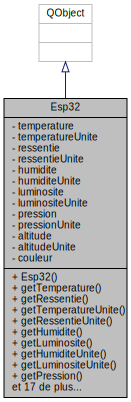
\includegraphics[width=203pt]{class_esp32__coll__graph}
\end{center}
\end{figure}
\subsubsection*{Fonctions membres publiques}
\begin{DoxyCompactItemize}
\item 
\hyperlink{class_esp32_abf9de8dee58d0105a551455874f29c19}{Esp32} (\hyperlink{class_q_object}{Q\+Object} $\ast$parent=nullptr)
\begin{DoxyCompactList}\small\item\em contructeur de la classe \hyperlink{class_esp32}{Esp32} \end{DoxyCompactList}\item 
double \hyperlink{class_esp32_adb339413686f3d78df1ecd41f106fd4e}{get\+Temperature} () const 
\begin{DoxyCompactList}\small\item\em retourne la valeur de temperature \end{DoxyCompactList}\item 
double \hyperlink{class_esp32_ae29854a5127d760a216f96ec7d797412}{get\+Ressentie} () const 
\begin{DoxyCompactList}\small\item\em retourne la valeur de ressentie \end{DoxyCompactList}\item 
Q\+String \hyperlink{class_esp32_ae20c976b79f87de083ca8ee49b2abf25}{get\+Temperature\+Unite} () const 
\begin{DoxyCompactList}\small\item\em retourne l\textquotesingle{}uniter de la valeur de temperature \end{DoxyCompactList}\item 
Q\+String \hyperlink{class_esp32_a548ed7533f742d087c65df256479ed00}{get\+Ressentie\+Unite} () const 
\begin{DoxyCompactList}\small\item\em retourne l\textquotesingle{}uniter de la valeur de ressentie \end{DoxyCompactList}\item 
int \hyperlink{class_esp32_a87f581ef8f01bcb71a7294cc545b242e}{get\+Humidite} () const 
\begin{DoxyCompactList}\small\item\em retourne la valeur d\textquotesingle{}humiditer \end{DoxyCompactList}\item 
int \hyperlink{class_esp32_aa2cdabace1ce70928c53d25e306a16d1}{get\+Luminosite} () const 
\begin{DoxyCompactList}\small\item\em retourne la valeur de luminositer \end{DoxyCompactList}\item 
Q\+String \hyperlink{class_esp32_ab2a1fc92c11af031814569f3d2836f33}{get\+Humidite\+Unite} () const 
\begin{DoxyCompactList}\small\item\em retourne l\textquotesingle{}uniter de la valeur d\textquotesingle{}humidite \end{DoxyCompactList}\item 
Q\+String \hyperlink{class_esp32_a50f4ef373379d2dbc0fd960438ab6f93}{get\+Luminosite\+Unite} () const 
\begin{DoxyCompactList}\small\item\em retourne l\textquotesingle{}uniter de la valeur de luminosite \end{DoxyCompactList}\item 
int \hyperlink{class_esp32_a31155a36108b37febae371d9ae65385a}{get\+Pression} () const 
\begin{DoxyCompactList}\small\item\em retourne la valeur de pression \end{DoxyCompactList}\item 
Q\+String \hyperlink{class_esp32_a398d4a1cbc61f7af2f3af7ecbcf2f93f}{get\+Pression\+Unite} () const 
\begin{DoxyCompactList}\small\item\em retourne l\textquotesingle{}uniter de la valeur de pression \end{DoxyCompactList}\item 
int \hyperlink{class_esp32_a31b691e6c75c1f9859bde4c0df8fe12f}{get\+Altitude} () const 
\begin{DoxyCompactList}\small\item\em retourne la valeur de l\textquotesingle{}altitude \end{DoxyCompactList}\item 
Q\+String \hyperlink{class_esp32_aad3c2e4b5d15a02abc62d0329f43942d}{get\+Altitude\+Unite} () const 
\begin{DoxyCompactList}\small\item\em retourne l\textquotesingle{}uniter de la valeur de l\textquotesingle{}altitude \end{DoxyCompactList}\item 
int \hyperlink{class_esp32_ac695656654b5d83ec3924b47f533f465}{get\+Etat\+Led} () const 
\begin{DoxyCompactList}\small\item\em retourne l\textquotesingle{}etat de la led \end{DoxyCompactList}\item 
void \hyperlink{class_esp32_a8e7a509ed5704bee4bc527ae297f14f0}{set\+Temperature} (double \hyperlink{class_esp32_a8274802633ca34c07fbfe7fa38a171a8}{temperature})
\begin{DoxyCompactList}\small\item\em modifie la variable température avec celle-\/ci passer en paramètre \end{DoxyCompactList}\item 
void \hyperlink{class_esp32_a85dc760b771c9233fa094a49679d9286}{set\+Ressentie} (double \hyperlink{class_esp32_a08425470633629dae05f61659ff90375}{ressentie})
\begin{DoxyCompactList}\small\item\em modifie la variable ressentie avec celle-\/ci passer en paramètre \end{DoxyCompactList}\item 
void \hyperlink{class_esp32_a709c261e1cea7b6bbd2ea1b09b1d7ec0}{set\+Temperature\+Unite} (Q\+String \hyperlink{class_esp32_a825526f0d6b74fda9ddeba7e67ec9dd5}{temperature\+Unite})
\begin{DoxyCompactList}\small\item\em modifie la variable de l\textquotesingle{}uniter utiliser pour la temperature \end{DoxyCompactList}\item 
void \hyperlink{class_esp32_abf8a7f9942150b6c17cc5d1cc7b0fc8a}{set\+Ressentie\+Unite} (Q\+String \hyperlink{class_esp32_a5333681c08a07f1877c20cfe88b7024f}{ressentie\+Unite})
\begin{DoxyCompactList}\small\item\em modifie la variable de l\textquotesingle{}uniter utiliser pour le ressentie \end{DoxyCompactList}\item 
void \hyperlink{class_esp32_a029c94bf405887eb890b3381ac176a9a}{set\+Humidite} (int \hyperlink{class_esp32_a7ad1a81c0a3cb29035aaef89d153f662}{humidite})
\begin{DoxyCompactList}\small\item\em modifie la variable de l\textquotesingle{}humidite \end{DoxyCompactList}\item 
void \hyperlink{class_esp32_ae60b48e8c808a5108402d5b9f03590ac}{set\+Luminosite} (int \hyperlink{class_esp32_aa6ce86f87c88d7fd29880e9865fefefc}{luminosite})
\begin{DoxyCompactList}\small\item\em modifie la variable de la luminosite \end{DoxyCompactList}\item 
void \hyperlink{class_esp32_ae9b2704f36bcd246668354d0ac06ea35}{set\+Humidite\+Unite} (Q\+String \hyperlink{class_esp32_a90c1ea9a5598c16a7918205185aa9fd6}{humidite\+Unite})
\begin{DoxyCompactList}\small\item\em modifie la variable de l\textquotesingle{}uniter utiliser pour l\textquotesingle{}humidite \end{DoxyCompactList}\item 
void \hyperlink{class_esp32_a36450bcd23e7676d1f0a46e8bec31275}{set\+Luminosite\+Unite} (Q\+String \hyperlink{class_esp32_a67087c5b6b76b64f929dbc255a7d5441}{luminosite\+Unite})
\begin{DoxyCompactList}\small\item\em modifie la variable de l\textquotesingle{}uniter utiliser pour la luminosite \end{DoxyCompactList}\item 
void \hyperlink{class_esp32_a583358abbf0b279dabb5a2976f1783de}{set\+Pression} (int \hyperlink{class_esp32_a7ddfb5679b439b204a93f775cfa9d2fa}{pression})
\begin{DoxyCompactList}\small\item\em modifie la variable de la pression \end{DoxyCompactList}\item 
void \hyperlink{class_esp32_a3c6dd57f955aef0738c48be705538337}{set\+Pression\+Unite} (Q\+String \hyperlink{class_esp32_aad1ead1e2c830025af0eebcdb30bcafe}{pression\+Unite})
\begin{DoxyCompactList}\small\item\em modifie la variable de l\textquotesingle{}uniter utiliser pour la pression \end{DoxyCompactList}\item 
void \hyperlink{class_esp32_aeb2268155501f27e36e6a7c6caa15412}{set\+Altitude} (int \hyperlink{class_esp32_ab257f7aff043b4d60d963e1bfd1fe35f}{altitude})
\begin{DoxyCompactList}\small\item\em modifie la variable altitude passer en paramètre \end{DoxyCompactList}\item 
void \hyperlink{class_esp32_a69b0c6a1c0a31e043b715be3fc40ded1}{set\+Altitude\+Unite} (Q\+String \hyperlink{class_esp32_ad407a4a4139183be7c4293fb254c96d7}{altitude\+Unite})
\begin{DoxyCompactList}\small\item\em modifie la variable de l\textquotesingle{}uniter utiliser pour l\textquotesingle{}altitude \end{DoxyCompactList}\item 
void \hyperlink{class_esp32_a32d0d1abb41a3762a54e9f5a33b3b247}{set\+Couleur\+Led} (int \hyperlink{class_esp32_ae8f6b2080769949ae5bd41c8312a6892}{couleur})
\begin{DoxyCompactList}\small\item\em modifie la variable de l\textquotesingle{}etat de la led \end{DoxyCompactList}\end{DoxyCompactItemize}
\subsubsection*{Attributs privés}
\begin{DoxyCompactItemize}
\item 
double \hyperlink{class_esp32_a8274802633ca34c07fbfe7fa38a171a8}{temperature}
\item 
Q\+String \hyperlink{class_esp32_a825526f0d6b74fda9ddeba7e67ec9dd5}{temperature\+Unite}
\item 
double \hyperlink{class_esp32_a08425470633629dae05f61659ff90375}{ressentie}
\item 
Q\+String \hyperlink{class_esp32_a5333681c08a07f1877c20cfe88b7024f}{ressentie\+Unite}
\item 
int \hyperlink{class_esp32_a7ad1a81c0a3cb29035aaef89d153f662}{humidite}
\item 
Q\+String \hyperlink{class_esp32_a90c1ea9a5598c16a7918205185aa9fd6}{humidite\+Unite}
\item 
int \hyperlink{class_esp32_aa6ce86f87c88d7fd29880e9865fefefc}{luminosite}
\item 
Q\+String \hyperlink{class_esp32_a67087c5b6b76b64f929dbc255a7d5441}{luminosite\+Unite}
\item 
int \hyperlink{class_esp32_a7ddfb5679b439b204a93f775cfa9d2fa}{pression}
\item 
Q\+String \hyperlink{class_esp32_aad1ead1e2c830025af0eebcdb30bcafe}{pression\+Unite}
\item 
int \hyperlink{class_esp32_ab257f7aff043b4d60d963e1bfd1fe35f}{altitude}
\item 
Q\+String \hyperlink{class_esp32_ad407a4a4139183be7c4293fb254c96d7}{altitude\+Unite}
\item 
int \hyperlink{class_esp32_ae8f6b2080769949ae5bd41c8312a6892}{couleur}
\end{DoxyCompactItemize}


\subsubsection{Documentation des constructeurs et destructeur}
\index{Esp32@{Esp32}!Esp32@{Esp32}}
\index{Esp32@{Esp32}!Esp32@{Esp32}}
\paragraph[{\texorpdfstring{Esp32(\+Q\+Object $\ast$parent=nullptr)}{Esp32(QObject *parent=nullptr)}}]{\setlength{\rightskip}{0pt plus 5cm}Esp32\+::\+Esp32 (
\begin{DoxyParamCaption}
\item[{{\bf Q\+Object} $\ast$}]{parent = {\ttfamily nullptr}}
\end{DoxyParamCaption}
)\hspace{0.3cm}{\ttfamily [explicit]}}\hypertarget{class_esp32_abf9de8dee58d0105a551455874f29c19}{}\label{class_esp32_abf9de8dee58d0105a551455874f29c19}

\begin{DoxyParams}{Paramètres}
{\em parent} & \\
\hline
\end{DoxyParams}

\begin{DoxyCode}
00021                             : \hyperlink{class_q_object}{QObject}(parent), \hyperlink{class_esp32_a8274802633ca34c07fbfe7fa38a171a8}{temperature}(0.), 
      \hyperlink{class_esp32_a825526f0d6b74fda9ddeba7e67ec9dd5}{temperatureUnite}(\textcolor{stringliteral}{"°C"}), \hyperlink{class_esp32_a08425470633629dae05f61659ff90375}{ressentie}(0.), \hyperlink{class_esp32_a5333681c08a07f1877c20cfe88b7024f}{ressentieUnite}(\textcolor{stringliteral}{"°C"}),
      \hyperlink{class_esp32_a7ad1a81c0a3cb29035aaef89d153f662}{\(\backslash\)}
00022 \hyperlink{class_esp32_a7ad1a81c0a3cb29035aaef89d153f662}{    humidite}(0), \hyperlink{class_esp32_a90c1ea9a5598c16a7918205185aa9fd6}{humiditeUnite}(\textcolor{stringliteral}{"%"}), \hyperlink{class_esp32_aa6ce86f87c88d7fd29880e9865fefefc}{luminosite}(0), 
      \hyperlink{class_esp32_a67087c5b6b76b64f929dbc255a7d5441}{luminositeUnite}(\textcolor{stringliteral}{"Lux"}), \hyperlink{class_esp32_a7ddfb5679b439b204a93f775cfa9d2fa}{pression}(0), \hyperlink{class_esp32_aad1ead1e2c830025af0eebcdb30bcafe}{pressionUnite}(\textcolor{stringliteral}{"hPa"}), 
      \hyperlink{class_esp32_ab257f7aff043b4d60d963e1bfd1fe35f}{altitude}(0), \hyperlink{class_esp32_ad407a4a4139183be7c4293fb254c96d7}{altitudeUnite}(\textcolor{stringliteral}{"Mètre"}), \hyperlink{class_esp32_ae8f6b2080769949ae5bd41c8312a6892}{couleur}(0)
00023 \{
00024 
00025 \}
\end{DoxyCode}


\subsubsection{Documentation des fonctions membres}
\index{Esp32@{Esp32}!get\+Altitude@{get\+Altitude}}
\index{get\+Altitude@{get\+Altitude}!Esp32@{Esp32}}
\paragraph[{\texorpdfstring{get\+Altitude() const }{getAltitude() const }}]{\setlength{\rightskip}{0pt plus 5cm}int Esp32\+::get\+Altitude (
\begin{DoxyParamCaption}
{}
\end{DoxyParamCaption}
) const}\hypertarget{class_esp32_a31b691e6c75c1f9859bde4c0df8fe12f}{}\label{class_esp32_a31b691e6c75c1f9859bde4c0df8fe12f}
recuperer l\textquotesingle{}unite de pression

\begin{DoxyReturn}{Renvoie}
int 
\end{DoxyReturn}


Références \hyperlink{class_esp32_ab257f7aff043b4d60d963e1bfd1fe35f}{altitude}.



Référencé par \hyperlink{class_ihm_a7c0a160f30e11a4f8d56b174e07566fe}{Ihm\+::actualiser\+Donnee()}.


\begin{DoxyCode}
00144 \{
00145     \textcolor{keywordflow}{return} \hyperlink{class_esp32_ab257f7aff043b4d60d963e1bfd1fe35f}{altitude};
00146 \}
\end{DoxyCode}
\index{Esp32@{Esp32}!get\+Altitude\+Unite@{get\+Altitude\+Unite}}
\index{get\+Altitude\+Unite@{get\+Altitude\+Unite}!Esp32@{Esp32}}
\paragraph[{\texorpdfstring{get\+Altitude\+Unite() const }{getAltitudeUnite() const }}]{\setlength{\rightskip}{0pt plus 5cm}Q\+String Esp32\+::get\+Altitude\+Unite (
\begin{DoxyParamCaption}
{}
\end{DoxyParamCaption}
) const}\hypertarget{class_esp32_aad3c2e4b5d15a02abc62d0329f43942d}{}\label{class_esp32_aad3c2e4b5d15a02abc62d0329f43942d}
recuperer l\textquotesingle{}altitude

\begin{DoxyReturn}{Renvoie}
Q\+String 
\end{DoxyReturn}


Références \hyperlink{class_esp32_ad407a4a4139183be7c4293fb254c96d7}{altitude\+Unite}.



Référencé par \hyperlink{class_ihm_a7c0a160f30e11a4f8d56b174e07566fe}{Ihm\+::actualiser\+Donnee()}.


\begin{DoxyCode}
00155 \{
00156     \textcolor{keywordflow}{return} \hyperlink{class_esp32_ad407a4a4139183be7c4293fb254c96d7}{altitudeUnite};
00157 \}
\end{DoxyCode}
\index{Esp32@{Esp32}!get\+Etat\+Led@{get\+Etat\+Led}}
\index{get\+Etat\+Led@{get\+Etat\+Led}!Esp32@{Esp32}}
\paragraph[{\texorpdfstring{get\+Etat\+Led() const }{getEtatLed() const }}]{\setlength{\rightskip}{0pt plus 5cm}int Esp32\+::get\+Etat\+Led (
\begin{DoxyParamCaption}
{}
\end{DoxyParamCaption}
) const}\hypertarget{class_esp32_ac695656654b5d83ec3924b47f533f465}{}\label{class_esp32_ac695656654b5d83ec3924b47f533f465}
recuperer l\textquotesingle{}unite d\textquotesingle{}altitude

\begin{DoxyReturn}{Renvoie}
int 
\end{DoxyReturn}


Références \hyperlink{class_esp32_ae8f6b2080769949ae5bd41c8312a6892}{couleur}.



Référencé par \hyperlink{class_ihm_af0426507c2130aefd01bdb4f825ae168}{Ihm\+::modifier\+Etat\+Led()}.


\begin{DoxyCode}
00166 \{
00167     \textcolor{keywordflow}{return} \hyperlink{class_esp32_ae8f6b2080769949ae5bd41c8312a6892}{couleur};
00168 \}
\end{DoxyCode}
\index{Esp32@{Esp32}!get\+Humidite@{get\+Humidite}}
\index{get\+Humidite@{get\+Humidite}!Esp32@{Esp32}}
\paragraph[{\texorpdfstring{get\+Humidite() const }{getHumidite() const }}]{\setlength{\rightskip}{0pt plus 5cm}int Esp32\+::get\+Humidite (
\begin{DoxyParamCaption}
{}
\end{DoxyParamCaption}
) const}\hypertarget{class_esp32_a87f581ef8f01bcb71a7294cc545b242e}{}\label{class_esp32_a87f581ef8f01bcb71a7294cc545b242e}
recuperer l\textquotesingle{}unite du resssentie

\begin{DoxyReturn}{Renvoie}
int 
\end{DoxyReturn}


Références \hyperlink{class_esp32_a7ad1a81c0a3cb29035aaef89d153f662}{humidite}.



Référencé par \hyperlink{class_ihm_a7c0a160f30e11a4f8d56b174e07566fe}{Ihm\+::actualiser\+Donnee()}.


\begin{DoxyCode}
00078 \{
00079     \textcolor{keywordflow}{return} \hyperlink{class_esp32_a7ad1a81c0a3cb29035aaef89d153f662}{humidite};
00080 \}
\end{DoxyCode}
\index{Esp32@{Esp32}!get\+Humidite\+Unite@{get\+Humidite\+Unite}}
\index{get\+Humidite\+Unite@{get\+Humidite\+Unite}!Esp32@{Esp32}}
\paragraph[{\texorpdfstring{get\+Humidite\+Unite() const }{getHumiditeUnite() const }}]{\setlength{\rightskip}{0pt plus 5cm}Q\+String Esp32\+::get\+Humidite\+Unite (
\begin{DoxyParamCaption}
{}
\end{DoxyParamCaption}
) const}\hypertarget{class_esp32_ab2a1fc92c11af031814569f3d2836f33}{}\label{class_esp32_ab2a1fc92c11af031814569f3d2836f33}
recuperer la luminosite

\begin{DoxyReturn}{Renvoie}
Q\+String 
\end{DoxyReturn}


Références \hyperlink{class_esp32_a90c1ea9a5598c16a7918205185aa9fd6}{humidite\+Unite}.



Référencé par \hyperlink{class_ihm_a7c0a160f30e11a4f8d56b174e07566fe}{Ihm\+::actualiser\+Donnee()}.


\begin{DoxyCode}
00100 \{
00101     \textcolor{keywordflow}{return} \hyperlink{class_esp32_a90c1ea9a5598c16a7918205185aa9fd6}{humiditeUnite};
00102 \}
\end{DoxyCode}
\index{Esp32@{Esp32}!get\+Luminosite@{get\+Luminosite}}
\index{get\+Luminosite@{get\+Luminosite}!Esp32@{Esp32}}
\paragraph[{\texorpdfstring{get\+Luminosite() const }{getLuminosite() const }}]{\setlength{\rightskip}{0pt plus 5cm}int Esp32\+::get\+Luminosite (
\begin{DoxyParamCaption}
{}
\end{DoxyParamCaption}
) const}\hypertarget{class_esp32_aa2cdabace1ce70928c53d25e306a16d1}{}\label{class_esp32_aa2cdabace1ce70928c53d25e306a16d1}
recuperer l\textquotesingle{}humidite

\begin{DoxyReturn}{Renvoie}
int 
\end{DoxyReturn}


Références \hyperlink{class_esp32_aa6ce86f87c88d7fd29880e9865fefefc}{luminosite}.



Référencé par \hyperlink{class_ihm_a7c0a160f30e11a4f8d56b174e07566fe}{Ihm\+::actualiser\+Donnee()}.


\begin{DoxyCode}
00089 \{
00090     \textcolor{keywordflow}{return} \hyperlink{class_esp32_aa6ce86f87c88d7fd29880e9865fefefc}{luminosite};
00091 \}
\end{DoxyCode}
\index{Esp32@{Esp32}!get\+Luminosite\+Unite@{get\+Luminosite\+Unite}}
\index{get\+Luminosite\+Unite@{get\+Luminosite\+Unite}!Esp32@{Esp32}}
\paragraph[{\texorpdfstring{get\+Luminosite\+Unite() const }{getLuminositeUnite() const }}]{\setlength{\rightskip}{0pt plus 5cm}Q\+String Esp32\+::get\+Luminosite\+Unite (
\begin{DoxyParamCaption}
{}
\end{DoxyParamCaption}
) const}\hypertarget{class_esp32_a50f4ef373379d2dbc0fd960438ab6f93}{}\label{class_esp32_a50f4ef373379d2dbc0fd960438ab6f93}
recuperer l\textquotesingle{}unite d\textquotesingle{}humidite

\begin{DoxyReturn}{Renvoie}
Q\+String 
\end{DoxyReturn}


Références \hyperlink{class_esp32_a67087c5b6b76b64f929dbc255a7d5441}{luminosite\+Unite}.



Référencé par \hyperlink{class_ihm_a7c0a160f30e11a4f8d56b174e07566fe}{Ihm\+::actualiser\+Donnee()}.


\begin{DoxyCode}
00111 \{
00112     \textcolor{keywordflow}{return} \hyperlink{class_esp32_a67087c5b6b76b64f929dbc255a7d5441}{luminositeUnite};
00113 \}
\end{DoxyCode}
\index{Esp32@{Esp32}!get\+Pression@{get\+Pression}}
\index{get\+Pression@{get\+Pression}!Esp32@{Esp32}}
\paragraph[{\texorpdfstring{get\+Pression() const }{getPression() const }}]{\setlength{\rightskip}{0pt plus 5cm}int Esp32\+::get\+Pression (
\begin{DoxyParamCaption}
{}
\end{DoxyParamCaption}
) const}\hypertarget{class_esp32_a31155a36108b37febae371d9ae65385a}{}\label{class_esp32_a31155a36108b37febae371d9ae65385a}
recuperer l\textquotesingle{}unite de luminosite

\begin{DoxyReturn}{Renvoie}
int 
\end{DoxyReturn}


Références \hyperlink{class_esp32_a7ddfb5679b439b204a93f775cfa9d2fa}{pression}.



Référencé par \hyperlink{class_ihm_a7c0a160f30e11a4f8d56b174e07566fe}{Ihm\+::actualiser\+Donnee()}.


\begin{DoxyCode}
00122 \{
00123     \textcolor{keywordflow}{return} \hyperlink{class_esp32_a7ddfb5679b439b204a93f775cfa9d2fa}{pression};
00124 \}
\end{DoxyCode}
\index{Esp32@{Esp32}!get\+Pression\+Unite@{get\+Pression\+Unite}}
\index{get\+Pression\+Unite@{get\+Pression\+Unite}!Esp32@{Esp32}}
\paragraph[{\texorpdfstring{get\+Pression\+Unite() const }{getPressionUnite() const }}]{\setlength{\rightskip}{0pt plus 5cm}Q\+String Esp32\+::get\+Pression\+Unite (
\begin{DoxyParamCaption}
{}
\end{DoxyParamCaption}
) const}\hypertarget{class_esp32_a398d4a1cbc61f7af2f3af7ecbcf2f93f}{}\label{class_esp32_a398d4a1cbc61f7af2f3af7ecbcf2f93f}
recuperer la pression

\begin{DoxyReturn}{Renvoie}
Q\+String 
\end{DoxyReturn}


Références \hyperlink{class_esp32_aad1ead1e2c830025af0eebcdb30bcafe}{pression\+Unite}.



Référencé par \hyperlink{class_ihm_a7c0a160f30e11a4f8d56b174e07566fe}{Ihm\+::actualiser\+Donnee()}.


\begin{DoxyCode}
00133 \{
00134     \textcolor{keywordflow}{return} \hyperlink{class_esp32_aad1ead1e2c830025af0eebcdb30bcafe}{pressionUnite};
00135 \}
\end{DoxyCode}
\index{Esp32@{Esp32}!get\+Ressentie@{get\+Ressentie}}
\index{get\+Ressentie@{get\+Ressentie}!Esp32@{Esp32}}
\paragraph[{\texorpdfstring{get\+Ressentie() const }{getRessentie() const }}]{\setlength{\rightskip}{0pt plus 5cm}double Esp32\+::get\+Ressentie (
\begin{DoxyParamCaption}
{}
\end{DoxyParamCaption}
) const}\hypertarget{class_esp32_ae29854a5127d760a216f96ec7d797412}{}\label{class_esp32_ae29854a5127d760a216f96ec7d797412}
recuperer la temperature

\begin{DoxyReturn}{Renvoie}
double 
\end{DoxyReturn}


Références \hyperlink{class_esp32_a08425470633629dae05f61659ff90375}{ressentie}.



Référencé par \hyperlink{class_ihm_a7c0a160f30e11a4f8d56b174e07566fe}{Ihm\+::actualiser\+Donnee()}.


\begin{DoxyCode}
00045 \{
00046     \textcolor{keywordflow}{return} \hyperlink{class_esp32_a08425470633629dae05f61659ff90375}{ressentie};
00047 \}
\end{DoxyCode}
\index{Esp32@{Esp32}!get\+Ressentie\+Unite@{get\+Ressentie\+Unite}}
\index{get\+Ressentie\+Unite@{get\+Ressentie\+Unite}!Esp32@{Esp32}}
\paragraph[{\texorpdfstring{get\+Ressentie\+Unite() const }{getRessentieUnite() const }}]{\setlength{\rightskip}{0pt plus 5cm}Q\+String Esp32\+::get\+Ressentie\+Unite (
\begin{DoxyParamCaption}
{}
\end{DoxyParamCaption}
) const}\hypertarget{class_esp32_a548ed7533f742d087c65df256479ed00}{}\label{class_esp32_a548ed7533f742d087c65df256479ed00}
recuperer l\textquotesingle{}unite de temperature

\begin{DoxyReturn}{Renvoie}
Q\+String 
\end{DoxyReturn}


Références \hyperlink{class_esp32_a5333681c08a07f1877c20cfe88b7024f}{ressentie\+Unite}.



Référencé par \hyperlink{class_ihm_a7c0a160f30e11a4f8d56b174e07566fe}{Ihm\+::actualiser\+Donnee()}.


\begin{DoxyCode}
00067 \{
00068     \textcolor{keywordflow}{return} \hyperlink{class_esp32_a5333681c08a07f1877c20cfe88b7024f}{ressentieUnite};
00069 \}
\end{DoxyCode}
\index{Esp32@{Esp32}!get\+Temperature@{get\+Temperature}}
\index{get\+Temperature@{get\+Temperature}!Esp32@{Esp32}}
\paragraph[{\texorpdfstring{get\+Temperature() const }{getTemperature() const }}]{\setlength{\rightskip}{0pt plus 5cm}double Esp32\+::get\+Temperature (
\begin{DoxyParamCaption}
{}
\end{DoxyParamCaption}
) const}\hypertarget{class_esp32_adb339413686f3d78df1ecd41f106fd4e}{}\label{class_esp32_adb339413686f3d78df1ecd41f106fd4e}
constructeur de la classe \hyperlink{class_esp32}{Esp32}

\begin{DoxyReturn}{Renvoie}
double ... 
\end{DoxyReturn}


Références \hyperlink{class_esp32_a8274802633ca34c07fbfe7fa38a171a8}{temperature}.



Référencé par \hyperlink{class_ihm_a7c0a160f30e11a4f8d56b174e07566fe}{Ihm\+::actualiser\+Donnee()}.


\begin{DoxyCode}
00034 \{
00035     \textcolor{keywordflow}{return} \hyperlink{class_esp32_a8274802633ca34c07fbfe7fa38a171a8}{temperature};
00036 \}
\end{DoxyCode}
\index{Esp32@{Esp32}!get\+Temperature\+Unite@{get\+Temperature\+Unite}}
\index{get\+Temperature\+Unite@{get\+Temperature\+Unite}!Esp32@{Esp32}}
\paragraph[{\texorpdfstring{get\+Temperature\+Unite() const }{getTemperatureUnite() const }}]{\setlength{\rightskip}{0pt plus 5cm}Q\+String Esp32\+::get\+Temperature\+Unite (
\begin{DoxyParamCaption}
{}
\end{DoxyParamCaption}
) const}\hypertarget{class_esp32_ae20c976b79f87de083ca8ee49b2abf25}{}\label{class_esp32_ae20c976b79f87de083ca8ee49b2abf25}
recuperer le ressentie

\begin{DoxyReturn}{Renvoie}
Q\+String 
\end{DoxyReturn}


Références \hyperlink{class_esp32_a825526f0d6b74fda9ddeba7e67ec9dd5}{temperature\+Unite}.



Référencé par \hyperlink{class_ihm_a7c0a160f30e11a4f8d56b174e07566fe}{Ihm\+::actualiser\+Donnee()}.


\begin{DoxyCode}
00056 \{
00057     \textcolor{keywordflow}{return} \hyperlink{class_esp32_a825526f0d6b74fda9ddeba7e67ec9dd5}{temperatureUnite};
00058 \}
\end{DoxyCode}
\index{Esp32@{Esp32}!set\+Altitude@{set\+Altitude}}
\index{set\+Altitude@{set\+Altitude}!Esp32@{Esp32}}
\paragraph[{\texorpdfstring{set\+Altitude(int altitude)}{setAltitude(int altitude)}}]{\setlength{\rightskip}{0pt plus 5cm}void Esp32\+::set\+Altitude (
\begin{DoxyParamCaption}
\item[{int}]{altitude}
\end{DoxyParamCaption}
)}\hypertarget{class_esp32_aeb2268155501f27e36e6a7c6caa15412}{}\label{class_esp32_aeb2268155501f27e36e6a7c6caa15412}
modifier la valeur de l\textquotesingle{}unite de pression


\begin{DoxyParams}{Paramètres}
{\em altitude} & \\
\hline
\end{DoxyParams}


Références \hyperlink{class_esp32_ab257f7aff043b4d60d963e1bfd1fe35f}{altitude}.



Référencé par \hyperlink{class_transmission_aa2977705ec793b10bf3212a13e67b097}{Transmission\+::decomposer()}.


\begin{DoxyCode}
00287 \{
00288     this->\hyperlink{class_esp32_ab257f7aff043b4d60d963e1bfd1fe35f}{altitude} = \hyperlink{class_esp32_ab257f7aff043b4d60d963e1bfd1fe35f}{altitude};
00289 \}
\end{DoxyCode}
\index{Esp32@{Esp32}!set\+Altitude\+Unite@{set\+Altitude\+Unite}}
\index{set\+Altitude\+Unite@{set\+Altitude\+Unite}!Esp32@{Esp32}}
\paragraph[{\texorpdfstring{set\+Altitude\+Unite(\+Q\+String altitude\+Unite)}{setAltitudeUnite(QString altitudeUnite)}}]{\setlength{\rightskip}{0pt plus 5cm}void Esp32\+::set\+Altitude\+Unite (
\begin{DoxyParamCaption}
\item[{Q\+String}]{altitude\+Unite}
\end{DoxyParamCaption}
)}\hypertarget{class_esp32_a69b0c6a1c0a31e043b715be3fc40ded1}{}\label{class_esp32_a69b0c6a1c0a31e043b715be3fc40ded1}
modifier la valeur d\textquotesingle{}altitude


\begin{DoxyParams}{Paramètres}
{\em altitude\+Unite} & \\
\hline
\end{DoxyParams}


Références \hyperlink{class_esp32_ad407a4a4139183be7c4293fb254c96d7}{altitude\+Unite}.



Référencé par \hyperlink{class_transmission_aa2977705ec793b10bf3212a13e67b097}{Transmission\+::decomposer()}.


\begin{DoxyCode}
00298 \{
00299     this->\hyperlink{class_esp32_ad407a4a4139183be7c4293fb254c96d7}{altitudeUnite} = \hyperlink{class_esp32_ad407a4a4139183be7c4293fb254c96d7}{altitudeUnite};
00300 \}
\end{DoxyCode}
\index{Esp32@{Esp32}!set\+Couleur\+Led@{set\+Couleur\+Led}}
\index{set\+Couleur\+Led@{set\+Couleur\+Led}!Esp32@{Esp32}}
\paragraph[{\texorpdfstring{set\+Couleur\+Led(int couleur)}{setCouleurLed(int couleur)}}]{\setlength{\rightskip}{0pt plus 5cm}void Esp32\+::set\+Couleur\+Led (
\begin{DoxyParamCaption}
\item[{int}]{couleur}
\end{DoxyParamCaption}
)}\hypertarget{class_esp32_a32d0d1abb41a3762a54e9f5a33b3b247}{}\label{class_esp32_a32d0d1abb41a3762a54e9f5a33b3b247}
modifier la valeur de l\textquotesingle{}unite altitude


\begin{DoxyParams}{Paramètres}
{\em couleur} & \\
\hline
\end{DoxyParams}


Références \hyperlink{class_esp32_ae8f6b2080769949ae5bd41c8312a6892}{couleur}.



Référencé par \hyperlink{class_transmission_aa2977705ec793b10bf3212a13e67b097}{Transmission\+::decomposer()}.


\begin{DoxyCode}
00308 \{
00309     this->\hyperlink{class_esp32_ae8f6b2080769949ae5bd41c8312a6892}{couleur} = \hyperlink{class_esp32_ae8f6b2080769949ae5bd41c8312a6892}{couleur};
00310 \}
\end{DoxyCode}
\index{Esp32@{Esp32}!set\+Humidite@{set\+Humidite}}
\index{set\+Humidite@{set\+Humidite}!Esp32@{Esp32}}
\paragraph[{\texorpdfstring{set\+Humidite(int humidite)}{setHumidite(int humidite)}}]{\setlength{\rightskip}{0pt plus 5cm}void Esp32\+::set\+Humidite (
\begin{DoxyParamCaption}
\item[{int}]{humidite}
\end{DoxyParamCaption}
)}\hypertarget{class_esp32_a029c94bf405887eb890b3381ac176a9a}{}\label{class_esp32_a029c94bf405887eb890b3381ac176a9a}
modifier la valeur de l\textquotesingle{}uniter de ressenti


\begin{DoxyParams}{Paramètres}
{\em humidite} & \\
\hline
\end{DoxyParams}


Références \hyperlink{class_esp32_a7ad1a81c0a3cb29035aaef89d153f662}{humidite}.



Référencé par \hyperlink{class_transmission_aa2977705ec793b10bf3212a13e67b097}{Transmission\+::decomposer()}.


\begin{DoxyCode}
00221 \{
00222     this->\hyperlink{class_esp32_a7ad1a81c0a3cb29035aaef89d153f662}{humidite} = \hyperlink{class_esp32_a7ad1a81c0a3cb29035aaef89d153f662}{humidite};
00223 \}
\end{DoxyCode}
\index{Esp32@{Esp32}!set\+Humidite\+Unite@{set\+Humidite\+Unite}}
\index{set\+Humidite\+Unite@{set\+Humidite\+Unite}!Esp32@{Esp32}}
\paragraph[{\texorpdfstring{set\+Humidite\+Unite(\+Q\+String humidite\+Unite)}{setHumiditeUnite(QString humiditeUnite)}}]{\setlength{\rightskip}{0pt plus 5cm}void Esp32\+::set\+Humidite\+Unite (
\begin{DoxyParamCaption}
\item[{Q\+String}]{humidite\+Unite}
\end{DoxyParamCaption}
)}\hypertarget{class_esp32_ae9b2704f36bcd246668354d0ac06ea35}{}\label{class_esp32_ae9b2704f36bcd246668354d0ac06ea35}
modifier la valeur de luminosite


\begin{DoxyParams}{Paramètres}
{\em humidite\+Unite} & \\
\hline
\end{DoxyParams}


Références \hyperlink{class_esp32_a90c1ea9a5598c16a7918205185aa9fd6}{humidite\+Unite}.



Référencé par \hyperlink{class_transmission_aa2977705ec793b10bf3212a13e67b097}{Transmission\+::decomposer()}.


\begin{DoxyCode}
00243 \{
00244     this->\hyperlink{class_esp32_a90c1ea9a5598c16a7918205185aa9fd6}{humiditeUnite} = \hyperlink{class_esp32_a90c1ea9a5598c16a7918205185aa9fd6}{humiditeUnite};
00245 \}
\end{DoxyCode}
\index{Esp32@{Esp32}!set\+Luminosite@{set\+Luminosite}}
\index{set\+Luminosite@{set\+Luminosite}!Esp32@{Esp32}}
\paragraph[{\texorpdfstring{set\+Luminosite(int luminosite)}{setLuminosite(int luminosite)}}]{\setlength{\rightskip}{0pt plus 5cm}void Esp32\+::set\+Luminosite (
\begin{DoxyParamCaption}
\item[{int}]{luminosite}
\end{DoxyParamCaption}
)}\hypertarget{class_esp32_ae60b48e8c808a5108402d5b9f03590ac}{}\label{class_esp32_ae60b48e8c808a5108402d5b9f03590ac}
modifier la valeur de l\textquotesingle{}humidite


\begin{DoxyParams}{Paramètres}
{\em luminosite} & \\
\hline
\end{DoxyParams}


Références \hyperlink{class_esp32_aa6ce86f87c88d7fd29880e9865fefefc}{luminosite}.



Référencé par \hyperlink{class_transmission_aa2977705ec793b10bf3212a13e67b097}{Transmission\+::decomposer()}.


\begin{DoxyCode}
00232 \{
00233     this->\hyperlink{class_esp32_aa6ce86f87c88d7fd29880e9865fefefc}{luminosite} = \hyperlink{class_esp32_aa6ce86f87c88d7fd29880e9865fefefc}{luminosite};
00234 \}
\end{DoxyCode}
\index{Esp32@{Esp32}!set\+Luminosite\+Unite@{set\+Luminosite\+Unite}}
\index{set\+Luminosite\+Unite@{set\+Luminosite\+Unite}!Esp32@{Esp32}}
\paragraph[{\texorpdfstring{set\+Luminosite\+Unite(\+Q\+String luminosite\+Unite)}{setLuminositeUnite(QString luminositeUnite)}}]{\setlength{\rightskip}{0pt plus 5cm}void Esp32\+::set\+Luminosite\+Unite (
\begin{DoxyParamCaption}
\item[{Q\+String}]{luminosite\+Unite}
\end{DoxyParamCaption}
)}\hypertarget{class_esp32_a36450bcd23e7676d1f0a46e8bec31275}{}\label{class_esp32_a36450bcd23e7676d1f0a46e8bec31275}
modifier la valeur de l\textquotesingle{}unite d\textquotesingle{}humidite


\begin{DoxyParams}{Paramètres}
{\em luminosite\+Unite} & \\
\hline
\end{DoxyParams}


Références \hyperlink{class_esp32_a67087c5b6b76b64f929dbc255a7d5441}{luminosite\+Unite}.



Référencé par \hyperlink{class_transmission_aa2977705ec793b10bf3212a13e67b097}{Transmission\+::decomposer()}.


\begin{DoxyCode}
00254 \{
00255     this->\hyperlink{class_esp32_a67087c5b6b76b64f929dbc255a7d5441}{luminositeUnite} = \hyperlink{class_esp32_a67087c5b6b76b64f929dbc255a7d5441}{luminositeUnite};
00256 \}
\end{DoxyCode}
\index{Esp32@{Esp32}!set\+Pression@{set\+Pression}}
\index{set\+Pression@{set\+Pression}!Esp32@{Esp32}}
\paragraph[{\texorpdfstring{set\+Pression(int pression)}{setPression(int pression)}}]{\setlength{\rightskip}{0pt plus 5cm}void Esp32\+::set\+Pression (
\begin{DoxyParamCaption}
\item[{int}]{pression}
\end{DoxyParamCaption}
)}\hypertarget{class_esp32_a583358abbf0b279dabb5a2976f1783de}{}\label{class_esp32_a583358abbf0b279dabb5a2976f1783de}
modifier la valeur de l\textquotesingle{}unite de luminosite


\begin{DoxyParams}{Paramètres}
{\em pression} & \\
\hline
\end{DoxyParams}


Références \hyperlink{class_esp32_a7ddfb5679b439b204a93f775cfa9d2fa}{pression}.



Référencé par \hyperlink{class_transmission_aa2977705ec793b10bf3212a13e67b097}{Transmission\+::decomposer()}.


\begin{DoxyCode}
00265 \{
00266     this->\hyperlink{class_esp32_a7ddfb5679b439b204a93f775cfa9d2fa}{pression} = \hyperlink{class_esp32_a7ddfb5679b439b204a93f775cfa9d2fa}{pression};
00267 \}
\end{DoxyCode}
\index{Esp32@{Esp32}!set\+Pression\+Unite@{set\+Pression\+Unite}}
\index{set\+Pression\+Unite@{set\+Pression\+Unite}!Esp32@{Esp32}}
\paragraph[{\texorpdfstring{set\+Pression\+Unite(\+Q\+String pression\+Unite)}{setPressionUnite(QString pressionUnite)}}]{\setlength{\rightskip}{0pt plus 5cm}void Esp32\+::set\+Pression\+Unite (
\begin{DoxyParamCaption}
\item[{Q\+String}]{pression\+Unite}
\end{DoxyParamCaption}
)}\hypertarget{class_esp32_a3c6dd57f955aef0738c48be705538337}{}\label{class_esp32_a3c6dd57f955aef0738c48be705538337}
modifier la valeur de la pression


\begin{DoxyParams}{Paramètres}
{\em pression\+Unite} & \\
\hline
\end{DoxyParams}


Références \hyperlink{class_esp32_aad1ead1e2c830025af0eebcdb30bcafe}{pression\+Unite}.



Référencé par \hyperlink{class_transmission_aa2977705ec793b10bf3212a13e67b097}{Transmission\+::decomposer()}.


\begin{DoxyCode}
00276 \{
00277     this->\hyperlink{class_esp32_aad1ead1e2c830025af0eebcdb30bcafe}{pressionUnite} = \hyperlink{class_esp32_aad1ead1e2c830025af0eebcdb30bcafe}{pressionUnite};
00278 \}
\end{DoxyCode}
\index{Esp32@{Esp32}!set\+Ressentie@{set\+Ressentie}}
\index{set\+Ressentie@{set\+Ressentie}!Esp32@{Esp32}}
\paragraph[{\texorpdfstring{set\+Ressentie(double ressentie)}{setRessentie(double ressentie)}}]{\setlength{\rightskip}{0pt plus 5cm}void Esp32\+::set\+Ressentie (
\begin{DoxyParamCaption}
\item[{double}]{ressentie}
\end{DoxyParamCaption}
)}\hypertarget{class_esp32_a85dc760b771c9233fa094a49679d9286}{}\label{class_esp32_a85dc760b771c9233fa094a49679d9286}
modifier la valeur de la temperature


\begin{DoxyParams}{Paramètres}
{\em ressentie} & \\
\hline
\end{DoxyParams}


Références \hyperlink{class_esp32_a08425470633629dae05f61659ff90375}{ressentie}.



Référencé par \hyperlink{class_transmission_aa2977705ec793b10bf3212a13e67b097}{Transmission\+::decomposer()}.


\begin{DoxyCode}
00188 \{
00189     this->\hyperlink{class_esp32_a08425470633629dae05f61659ff90375}{ressentie} = \hyperlink{class_esp32_a08425470633629dae05f61659ff90375}{ressentie};
00190 \}
\end{DoxyCode}
\index{Esp32@{Esp32}!set\+Ressentie\+Unite@{set\+Ressentie\+Unite}}
\index{set\+Ressentie\+Unite@{set\+Ressentie\+Unite}!Esp32@{Esp32}}
\paragraph[{\texorpdfstring{set\+Ressentie\+Unite(\+Q\+String ressentie\+Unite)}{setRessentieUnite(QString ressentieUnite)}}]{\setlength{\rightskip}{0pt plus 5cm}void Esp32\+::set\+Ressentie\+Unite (
\begin{DoxyParamCaption}
\item[{Q\+String}]{ressentie\+Unite}
\end{DoxyParamCaption}
)}\hypertarget{class_esp32_abf8a7f9942150b6c17cc5d1cc7b0fc8a}{}\label{class_esp32_abf8a7f9942150b6c17cc5d1cc7b0fc8a}
modifier la valeur de l\textquotesingle{}uniter de temperature


\begin{DoxyParams}{Paramètres}
{\em ressentie\+Unite} & \\
\hline
\end{DoxyParams}


Références \hyperlink{class_esp32_a5333681c08a07f1877c20cfe88b7024f}{ressentie\+Unite}.



Référencé par \hyperlink{class_transmission_aa2977705ec793b10bf3212a13e67b097}{Transmission\+::decomposer()}.


\begin{DoxyCode}
00210 \{
00211     this->\hyperlink{class_esp32_a5333681c08a07f1877c20cfe88b7024f}{ressentieUnite} = \textcolor{stringliteral}{"°"} + \hyperlink{class_esp32_a5333681c08a07f1877c20cfe88b7024f}{ressentieUnite};
00212 \}
\end{DoxyCode}
\index{Esp32@{Esp32}!set\+Temperature@{set\+Temperature}}
\index{set\+Temperature@{set\+Temperature}!Esp32@{Esp32}}
\paragraph[{\texorpdfstring{set\+Temperature(double temperature)}{setTemperature(double temperature)}}]{\setlength{\rightskip}{0pt plus 5cm}void Esp32\+::set\+Temperature (
\begin{DoxyParamCaption}
\item[{double}]{temperature}
\end{DoxyParamCaption}
)}\hypertarget{class_esp32_a8e7a509ed5704bee4bc527ae297f14f0}{}\label{class_esp32_a8e7a509ed5704bee4bc527ae297f14f0}
recuperer l\textquotesingle{}etat de la led


\begin{DoxyParams}{Paramètres}
{\em temperature} & \\
\hline
\end{DoxyParams}


Références \hyperlink{class_esp32_a8274802633ca34c07fbfe7fa38a171a8}{temperature}.



Référencé par \hyperlink{class_transmission_aa2977705ec793b10bf3212a13e67b097}{Transmission\+::decomposer()}.


\begin{DoxyCode}
00177 \{
00178     this->\hyperlink{class_esp32_a8274802633ca34c07fbfe7fa38a171a8}{temperature} = \hyperlink{class_esp32_a8274802633ca34c07fbfe7fa38a171a8}{temperature};
00179 \}
\end{DoxyCode}
\index{Esp32@{Esp32}!set\+Temperature\+Unite@{set\+Temperature\+Unite}}
\index{set\+Temperature\+Unite@{set\+Temperature\+Unite}!Esp32@{Esp32}}
\paragraph[{\texorpdfstring{set\+Temperature\+Unite(\+Q\+String temperature\+Unite)}{setTemperatureUnite(QString temperatureUnite)}}]{\setlength{\rightskip}{0pt plus 5cm}void Esp32\+::set\+Temperature\+Unite (
\begin{DoxyParamCaption}
\item[{Q\+String}]{temperature\+Unite}
\end{DoxyParamCaption}
)}\hypertarget{class_esp32_a709c261e1cea7b6bbd2ea1b09b1d7ec0}{}\label{class_esp32_a709c261e1cea7b6bbd2ea1b09b1d7ec0}
modifier la valeur de ressenti


\begin{DoxyParams}{Paramètres}
{\em temperature\+Unite} & \\
\hline
\end{DoxyParams}


Références \hyperlink{class_esp32_a825526f0d6b74fda9ddeba7e67ec9dd5}{temperature\+Unite}.



Référencé par \hyperlink{class_transmission_aa2977705ec793b10bf3212a13e67b097}{Transmission\+::decomposer()}.


\begin{DoxyCode}
00199 \{
00200     this->\hyperlink{class_esp32_a825526f0d6b74fda9ddeba7e67ec9dd5}{temperatureUnite} = \textcolor{stringliteral}{"°"} + \hyperlink{class_esp32_a825526f0d6b74fda9ddeba7e67ec9dd5}{temperatureUnite};
00201 \}
\end{DoxyCode}


\subsubsection{Documentation des données membres}
\index{Esp32@{Esp32}!altitude@{altitude}}
\index{altitude@{altitude}!Esp32@{Esp32}}
\paragraph[{\texorpdfstring{altitude}{altitude}}]{\setlength{\rightskip}{0pt plus 5cm}int Esp32\+::altitude\hspace{0.3cm}{\ttfamily [private]}}\hypertarget{class_esp32_ab257f7aff043b4d60d963e1bfd1fe35f}{}\label{class_esp32_ab257f7aff043b4d60d963e1bfd1fe35f}
variable qui stocke l\textquotesingle{}unite de pression 

Référencé par \hyperlink{class_esp32_a31b691e6c75c1f9859bde4c0df8fe12f}{get\+Altitude()}, et \hyperlink{class_esp32_aeb2268155501f27e36e6a7c6caa15412}{set\+Altitude()}.

\index{Esp32@{Esp32}!altitude\+Unite@{altitude\+Unite}}
\index{altitude\+Unite@{altitude\+Unite}!Esp32@{Esp32}}
\paragraph[{\texorpdfstring{altitude\+Unite}{altitudeUnite}}]{\setlength{\rightskip}{0pt plus 5cm}Q\+String Esp32\+::altitude\+Unite\hspace{0.3cm}{\ttfamily [private]}}\hypertarget{class_esp32_ad407a4a4139183be7c4293fb254c96d7}{}\label{class_esp32_ad407a4a4139183be7c4293fb254c96d7}
variable qui stocke l\textquotesingle{}altitude 

Référencé par \hyperlink{class_esp32_aad3c2e4b5d15a02abc62d0329f43942d}{get\+Altitude\+Unite()}, et \hyperlink{class_esp32_a69b0c6a1c0a31e043b715be3fc40ded1}{set\+Altitude\+Unite()}.

\index{Esp32@{Esp32}!couleur@{couleur}}
\index{couleur@{couleur}!Esp32@{Esp32}}
\paragraph[{\texorpdfstring{couleur}{couleur}}]{\setlength{\rightskip}{0pt plus 5cm}int Esp32\+::couleur\hspace{0.3cm}{\ttfamily [private]}}\hypertarget{class_esp32_ae8f6b2080769949ae5bd41c8312a6892}{}\label{class_esp32_ae8f6b2080769949ae5bd41c8312a6892}
variable qui stocke l\textquotesingle{}unite de l\textquotesingle{}altitude 

Référencé par \hyperlink{class_esp32_ac695656654b5d83ec3924b47f533f465}{get\+Etat\+Led()}, et \hyperlink{class_esp32_a32d0d1abb41a3762a54e9f5a33b3b247}{set\+Couleur\+Led()}.

\index{Esp32@{Esp32}!humidite@{humidite}}
\index{humidite@{humidite}!Esp32@{Esp32}}
\paragraph[{\texorpdfstring{humidite}{humidite}}]{\setlength{\rightskip}{0pt plus 5cm}int Esp32\+::humidite\hspace{0.3cm}{\ttfamily [private]}}\hypertarget{class_esp32_a7ad1a81c0a3cb29035aaef89d153f662}{}\label{class_esp32_a7ad1a81c0a3cb29035aaef89d153f662}
variable qui stocke l\textquotesingle{}unite de ressenti 

Référencé par \hyperlink{class_esp32_a87f581ef8f01bcb71a7294cc545b242e}{get\+Humidite()}, et \hyperlink{class_esp32_a029c94bf405887eb890b3381ac176a9a}{set\+Humidite()}.

\index{Esp32@{Esp32}!humidite\+Unite@{humidite\+Unite}}
\index{humidite\+Unite@{humidite\+Unite}!Esp32@{Esp32}}
\paragraph[{\texorpdfstring{humidite\+Unite}{humiditeUnite}}]{\setlength{\rightskip}{0pt plus 5cm}Q\+String Esp32\+::humidite\+Unite\hspace{0.3cm}{\ttfamily [private]}}\hypertarget{class_esp32_a90c1ea9a5598c16a7918205185aa9fd6}{}\label{class_esp32_a90c1ea9a5598c16a7918205185aa9fd6}
variable qui stocke l\textquotesingle{}humidite 

Référencé par \hyperlink{class_esp32_ab2a1fc92c11af031814569f3d2836f33}{get\+Humidite\+Unite()}, et \hyperlink{class_esp32_ae9b2704f36bcd246668354d0ac06ea35}{set\+Humidite\+Unite()}.

\index{Esp32@{Esp32}!luminosite@{luminosite}}
\index{luminosite@{luminosite}!Esp32@{Esp32}}
\paragraph[{\texorpdfstring{luminosite}{luminosite}}]{\setlength{\rightskip}{0pt plus 5cm}int Esp32\+::luminosite\hspace{0.3cm}{\ttfamily [private]}}\hypertarget{class_esp32_aa6ce86f87c88d7fd29880e9865fefefc}{}\label{class_esp32_aa6ce86f87c88d7fd29880e9865fefefc}
variable qui stocke l\textquotesingle{}unite de l\textquotesingle{}humidite 

Référencé par \hyperlink{class_esp32_aa2cdabace1ce70928c53d25e306a16d1}{get\+Luminosite()}, et \hyperlink{class_esp32_ae60b48e8c808a5108402d5b9f03590ac}{set\+Luminosite()}.

\index{Esp32@{Esp32}!luminosite\+Unite@{luminosite\+Unite}}
\index{luminosite\+Unite@{luminosite\+Unite}!Esp32@{Esp32}}
\paragraph[{\texorpdfstring{luminosite\+Unite}{luminositeUnite}}]{\setlength{\rightskip}{0pt plus 5cm}Q\+String Esp32\+::luminosite\+Unite\hspace{0.3cm}{\ttfamily [private]}}\hypertarget{class_esp32_a67087c5b6b76b64f929dbc255a7d5441}{}\label{class_esp32_a67087c5b6b76b64f929dbc255a7d5441}
variable qui stocke la luminosite 

Référencé par \hyperlink{class_esp32_a50f4ef373379d2dbc0fd960438ab6f93}{get\+Luminosite\+Unite()}, et \hyperlink{class_esp32_a36450bcd23e7676d1f0a46e8bec31275}{set\+Luminosite\+Unite()}.

\index{Esp32@{Esp32}!pression@{pression}}
\index{pression@{pression}!Esp32@{Esp32}}
\paragraph[{\texorpdfstring{pression}{pression}}]{\setlength{\rightskip}{0pt plus 5cm}int Esp32\+::pression\hspace{0.3cm}{\ttfamily [private]}}\hypertarget{class_esp32_a7ddfb5679b439b204a93f775cfa9d2fa}{}\label{class_esp32_a7ddfb5679b439b204a93f775cfa9d2fa}
variable qui stocke l\textquotesingle{}unite de la luminosite 

Référencé par \hyperlink{class_esp32_a31155a36108b37febae371d9ae65385a}{get\+Pression()}, et \hyperlink{class_esp32_a583358abbf0b279dabb5a2976f1783de}{set\+Pression()}.

\index{Esp32@{Esp32}!pression\+Unite@{pression\+Unite}}
\index{pression\+Unite@{pression\+Unite}!Esp32@{Esp32}}
\paragraph[{\texorpdfstring{pression\+Unite}{pressionUnite}}]{\setlength{\rightskip}{0pt plus 5cm}Q\+String Esp32\+::pression\+Unite\hspace{0.3cm}{\ttfamily [private]}}\hypertarget{class_esp32_aad1ead1e2c830025af0eebcdb30bcafe}{}\label{class_esp32_aad1ead1e2c830025af0eebcdb30bcafe}
variable qui stocke la pression 

Référencé par \hyperlink{class_esp32_a398d4a1cbc61f7af2f3af7ecbcf2f93f}{get\+Pression\+Unite()}, et \hyperlink{class_esp32_a3c6dd57f955aef0738c48be705538337}{set\+Pression\+Unite()}.

\index{Esp32@{Esp32}!ressentie@{ressentie}}
\index{ressentie@{ressentie}!Esp32@{Esp32}}
\paragraph[{\texorpdfstring{ressentie}{ressentie}}]{\setlength{\rightskip}{0pt plus 5cm}double Esp32\+::ressentie\hspace{0.3cm}{\ttfamily [private]}}\hypertarget{class_esp32_a08425470633629dae05f61659ff90375}{}\label{class_esp32_a08425470633629dae05f61659ff90375}
variable qui stocke l\textquotesingle{}unite de la temperature 

Référencé par \hyperlink{class_esp32_ae29854a5127d760a216f96ec7d797412}{get\+Ressentie()}, et \hyperlink{class_esp32_a85dc760b771c9233fa094a49679d9286}{set\+Ressentie()}.

\index{Esp32@{Esp32}!ressentie\+Unite@{ressentie\+Unite}}
\index{ressentie\+Unite@{ressentie\+Unite}!Esp32@{Esp32}}
\paragraph[{\texorpdfstring{ressentie\+Unite}{ressentieUnite}}]{\setlength{\rightskip}{0pt plus 5cm}Q\+String Esp32\+::ressentie\+Unite\hspace{0.3cm}{\ttfamily [private]}}\hypertarget{class_esp32_a5333681c08a07f1877c20cfe88b7024f}{}\label{class_esp32_a5333681c08a07f1877c20cfe88b7024f}
variable qui stocke le ressenti 

Référencé par \hyperlink{class_esp32_a548ed7533f742d087c65df256479ed00}{get\+Ressentie\+Unite()}, et \hyperlink{class_esp32_abf8a7f9942150b6c17cc5d1cc7b0fc8a}{set\+Ressentie\+Unite()}.

\index{Esp32@{Esp32}!temperature@{temperature}}
\index{temperature@{temperature}!Esp32@{Esp32}}
\paragraph[{\texorpdfstring{temperature}{temperature}}]{\setlength{\rightskip}{0pt plus 5cm}double Esp32\+::temperature\hspace{0.3cm}{\ttfamily [private]}}\hypertarget{class_esp32_a8274802633ca34c07fbfe7fa38a171a8}{}\label{class_esp32_a8274802633ca34c07fbfe7fa38a171a8}
modifier l\textquotesingle{}etat de la led 

Référencé par \hyperlink{class_esp32_adb339413686f3d78df1ecd41f106fd4e}{get\+Temperature()}, et \hyperlink{class_esp32_a8e7a509ed5704bee4bc527ae297f14f0}{set\+Temperature()}.

\index{Esp32@{Esp32}!temperature\+Unite@{temperature\+Unite}}
\index{temperature\+Unite@{temperature\+Unite}!Esp32@{Esp32}}
\paragraph[{\texorpdfstring{temperature\+Unite}{temperatureUnite}}]{\setlength{\rightskip}{0pt plus 5cm}Q\+String Esp32\+::temperature\+Unite\hspace{0.3cm}{\ttfamily [private]}}\hypertarget{class_esp32_a825526f0d6b74fda9ddeba7e67ec9dd5}{}\label{class_esp32_a825526f0d6b74fda9ddeba7e67ec9dd5}
variable qui stocke la temperature 

Référencé par \hyperlink{class_esp32_ae20c976b79f87de083ca8ee49b2abf25}{get\+Temperature\+Unite()}, et \hyperlink{class_esp32_a709c261e1cea7b6bbd2ea1b09b1d7ec0}{set\+Temperature\+Unite()}.



La documentation de cette classe a été générée à partir des fichiers suivants \+:\begin{DoxyCompactItemize}
\item 
\hyperlink{esp32_8h}{esp32.\+h}\item 
\hyperlink{esp32_8cpp}{esp32.\+cpp}\end{DoxyCompactItemize}

\hypertarget{class_gps}{}\subsection{Référence de la classe Gps}
\label{class_gps}\index{Gps@{Gps}}


Declaration de la classe \hyperlink{class_gps}{Gps}.  




{\ttfamily \#include \char`\"{}gps.\+h\char`\"{}}



Graphe de collaboration de Gps\+:\nopagebreak
\begin{figure}[H]
\begin{center}
\leavevmode
\includegraphics[width=167pt]{class_gps__coll__graph}
\end{center}
\end{figure}
\subsubsection*{Fonctions membres publiques}
\begin{DoxyCompactItemize}
\item 
\hyperlink{class_gps_a10a73359b33c1357564ebc83fc078000}{Gps} ()
\begin{DoxyCompactList}\small\item\em constructeur de la classe \hyperlink{class_gps}{Gps} \end{DoxyCompactList}\item 
\hyperlink{class_gps_a9f076d88f081ae5c010cf150cb957b66}{$\sim$\+Gps} ()
\begin{DoxyCompactList}\small\item\em destructeur de la classe \hyperlink{class_gps}{Gps} \end{DoxyCompactList}\item 
double \hyperlink{class_gps_a44c6469bf67727853c06d4be037c6b0f}{get\+Latitude} () const 
\begin{DoxyCompactList}\small\item\em return la valeur de la latitude \end{DoxyCompactList}\item 
double \hyperlink{class_gps_a6ce8da770e213bfbf7f204b107d9e3f5}{get\+Longitude} () const 
\begin{DoxyCompactList}\small\item\em return la valeur de la longitude \end{DoxyCompactList}\item 
void \hyperlink{class_gps_aaabf328f0bbcdbb9c2901e30b6edccc7}{set\+Latitude} (double \hyperlink{class_gps_a2457bce0fe69afbf68c27a4807c3f847}{latitude})
\begin{DoxyCompactList}\small\item\em modifier la valeur de la latitude \end{DoxyCompactList}\item 
void \hyperlink{class_gps_a2d9ca07c62c5bae627c2131062a1236a}{set\+Longitude} (double \hyperlink{class_gps_a6e56fa2b9f1402901a0c768b796402ce}{longitude})
\begin{DoxyCompactList}\small\item\em modifier la valeur de la longitude \end{DoxyCompactList}\end{DoxyCompactItemize}
\subsubsection*{Attributs privés}
\begin{DoxyCompactItemize}
\item 
double \hyperlink{class_gps_a2457bce0fe69afbf68c27a4807c3f847}{latitude}
\item 
double \hyperlink{class_gps_a6e56fa2b9f1402901a0c768b796402ce}{longitude}
\end{DoxyCompactItemize}


\subsubsection{Documentation des constructeurs et destructeur}
\index{Gps@{Gps}!Gps@{Gps}}
\index{Gps@{Gps}!Gps@{Gps}}
\paragraph[{\texorpdfstring{Gps()}{Gps()}}]{\setlength{\rightskip}{0pt plus 5cm}Gps\+::\+Gps (
\begin{DoxyParamCaption}
{}
\end{DoxyParamCaption}
)}\hypertarget{class_gps_a10a73359b33c1357564ebc83fc078000}{}\label{class_gps_a10a73359b33c1357564ebc83fc078000}

\begin{DoxyCode}
00020         : \hyperlink{class_gps_a2457bce0fe69afbf68c27a4807c3f847}{latitude}(0.), \hyperlink{class_gps_a6e56fa2b9f1402901a0c768b796402ce}{longitude}(0.)
00021 \{
00022 
00023 \}
\end{DoxyCode}
\index{Gps@{Gps}!````~Gps@{$\sim$\+Gps}}
\index{````~Gps@{$\sim$\+Gps}!Gps@{Gps}}
\paragraph[{\texorpdfstring{$\sim$\+Gps()}{~Gps()}}]{\setlength{\rightskip}{0pt plus 5cm}Gps\+::$\sim$\+Gps (
\begin{DoxyParamCaption}
{}
\end{DoxyParamCaption}
)}\hypertarget{class_gps_a9f076d88f081ae5c010cf150cb957b66}{}\label{class_gps_a9f076d88f081ae5c010cf150cb957b66}
constructeur de la classe \hyperlink{class_gps}{Gps} 
\begin{DoxyCode}
00031 \{
00032 
00033 \}
\end{DoxyCode}


\subsubsection{Documentation des fonctions membres}
\index{Gps@{Gps}!get\+Latitude@{get\+Latitude}}
\index{get\+Latitude@{get\+Latitude}!Gps@{Gps}}
\paragraph[{\texorpdfstring{get\+Latitude() const }{getLatitude() const }}]{\setlength{\rightskip}{0pt plus 5cm}double Gps\+::get\+Latitude (
\begin{DoxyParamCaption}
{}
\end{DoxyParamCaption}
) const}\hypertarget{class_gps_a44c6469bf67727853c06d4be037c6b0f}{}\label{class_gps_a44c6469bf67727853c06d4be037c6b0f}
destructeur de la classe \hyperlink{class_gps}{Gps}

\begin{DoxyReturn}{Renvoie}
double 
\end{DoxyReturn}


Références \hyperlink{class_gps_a2457bce0fe69afbf68c27a4807c3f847}{latitude}.



Référencé par \hyperlink{class_ihm_a3ca276093d65c42a5fc5a87cbca1972a}{Ihm\+::actualiser\+Donnee\+Gps()}, et \hyperlink{class_ihm_a850d1c97ed5fe5ba3cf3aa85d81872cd}{Ihm\+::on\+\_\+push\+Button\+Envoyer\+Coordonnee\+\_\+clicked()}.


\begin{DoxyCode}
00053 \{
00054     \textcolor{keywordflow}{return} \hyperlink{class_gps_a2457bce0fe69afbf68c27a4807c3f847}{latitude};
00055 \}
\end{DoxyCode}
\index{Gps@{Gps}!get\+Longitude@{get\+Longitude}}
\index{get\+Longitude@{get\+Longitude}!Gps@{Gps}}
\paragraph[{\texorpdfstring{get\+Longitude() const }{getLongitude() const }}]{\setlength{\rightskip}{0pt plus 5cm}double Gps\+::get\+Longitude (
\begin{DoxyParamCaption}
{}
\end{DoxyParamCaption}
) const}\hypertarget{class_gps_a6ce8da770e213bfbf7f204b107d9e3f5}{}\label{class_gps_a6ce8da770e213bfbf7f204b107d9e3f5}
recuperer la latitude

\begin{DoxyReturn}{Renvoie}
double 
\end{DoxyReturn}


Références \hyperlink{class_gps_a6e56fa2b9f1402901a0c768b796402ce}{longitude}.



Référencé par \hyperlink{class_ihm_a3ca276093d65c42a5fc5a87cbca1972a}{Ihm\+::actualiser\+Donnee\+Gps()}, et \hyperlink{class_ihm_a850d1c97ed5fe5ba3cf3aa85d81872cd}{Ihm\+::on\+\_\+push\+Button\+Envoyer\+Coordonnee\+\_\+clicked()}.


\begin{DoxyCode}
00042 \{
00043     \textcolor{keywordflow}{return} \hyperlink{class_gps_a6e56fa2b9f1402901a0c768b796402ce}{longitude};
00044 \}
\end{DoxyCode}
\index{Gps@{Gps}!set\+Latitude@{set\+Latitude}}
\index{set\+Latitude@{set\+Latitude}!Gps@{Gps}}
\paragraph[{\texorpdfstring{set\+Latitude(double latitude)}{setLatitude(double latitude)}}]{\setlength{\rightskip}{0pt plus 5cm}void Gps\+::set\+Latitude (
\begin{DoxyParamCaption}
\item[{double}]{latitude}
\end{DoxyParamCaption}
)}\hypertarget{class_gps_aaabf328f0bbcdbb9c2901e30b6edccc7}{}\label{class_gps_aaabf328f0bbcdbb9c2901e30b6edccc7}
recuperer la longitune


\begin{DoxyParams}{Paramètres}
{\em latitude} & \\
\hline
\end{DoxyParams}


Références \hyperlink{class_gps_a2457bce0fe69afbf68c27a4807c3f847}{latitude}.



Référencé par \hyperlink{class_transmission_acc25e99cce910d23efe684cad233d30e}{Transmission\+::decomposer\+Donnee\+Gps()}.


\begin{DoxyCode}
00064 \{
00065     this->\hyperlink{class_gps_a2457bce0fe69afbf68c27a4807c3f847}{latitude} = \hyperlink{class_gps_a2457bce0fe69afbf68c27a4807c3f847}{latitude};
00066 \}
\end{DoxyCode}
\index{Gps@{Gps}!set\+Longitude@{set\+Longitude}}
\index{set\+Longitude@{set\+Longitude}!Gps@{Gps}}
\paragraph[{\texorpdfstring{set\+Longitude(double longitude)}{setLongitude(double longitude)}}]{\setlength{\rightskip}{0pt plus 5cm}void Gps\+::set\+Longitude (
\begin{DoxyParamCaption}
\item[{double}]{longitude}
\end{DoxyParamCaption}
)}\hypertarget{class_gps_a2d9ca07c62c5bae627c2131062a1236a}{}\label{class_gps_a2d9ca07c62c5bae627c2131062a1236a}
modifier la valeur de la latitude


\begin{DoxyParams}{Paramètres}
{\em longitude} & \\
\hline
\end{DoxyParams}


Références \hyperlink{class_gps_a6e56fa2b9f1402901a0c768b796402ce}{longitude}.



Référencé par \hyperlink{class_transmission_acc25e99cce910d23efe684cad233d30e}{Transmission\+::decomposer\+Donnee\+Gps()}.


\begin{DoxyCode}
00075 \{
00076     this->\hyperlink{class_gps_a6e56fa2b9f1402901a0c768b796402ce}{longitude} = \hyperlink{class_gps_a6e56fa2b9f1402901a0c768b796402ce}{longitude};
00077 \}
\end{DoxyCode}


\subsubsection{Documentation des données membres}
\index{Gps@{Gps}!latitude@{latitude}}
\index{latitude@{latitude}!Gps@{Gps}}
\paragraph[{\texorpdfstring{latitude}{latitude}}]{\setlength{\rightskip}{0pt plus 5cm}double Gps\+::latitude\hspace{0.3cm}{\ttfamily [private]}}\hypertarget{class_gps_a2457bce0fe69afbf68c27a4807c3f847}{}\label{class_gps_a2457bce0fe69afbf68c27a4807c3f847}
modifier la valeur de la longitude 

Référencé par \hyperlink{class_gps_a44c6469bf67727853c06d4be037c6b0f}{get\+Latitude()}, et \hyperlink{class_gps_aaabf328f0bbcdbb9c2901e30b6edccc7}{set\+Latitude()}.

\index{Gps@{Gps}!longitude@{longitude}}
\index{longitude@{longitude}!Gps@{Gps}}
\paragraph[{\texorpdfstring{longitude}{longitude}}]{\setlength{\rightskip}{0pt plus 5cm}double Gps\+::longitude\hspace{0.3cm}{\ttfamily [private]}}\hypertarget{class_gps_a6e56fa2b9f1402901a0c768b796402ce}{}\label{class_gps_a6e56fa2b9f1402901a0c768b796402ce}
variable qui stocke la latitude 

Référencé par \hyperlink{class_gps_a6ce8da770e213bfbf7f204b107d9e3f5}{get\+Longitude()}, et \hyperlink{class_gps_a2d9ca07c62c5bae627c2131062a1236a}{set\+Longitude()}.



La documentation de cette classe a été générée à partir des fichiers suivants \+:\begin{DoxyCompactItemize}
\item 
\hyperlink{gps_8h}{gps.\+h}\item 
\hyperlink{gps_8cpp}{gps.\+cpp}\end{DoxyCompactItemize}

\hypertarget{class_graphique}{}\subsection{Référence de la classe Graphique}
\label{class_graphique}\index{Graphique@{Graphique}}


Declaration de la classe \hyperlink{class_graphique}{Graphique}.  




{\ttfamily \#include \char`\"{}graphique.\+h\char`\"{}}



Graphe de collaboration de Graphique\+:\nopagebreak
\begin{figure}[H]
\begin{center}
\leavevmode
\includegraphics[width=232pt]{class_graphique__coll__graph}
\end{center}
\end{figure}
\subsubsection*{Fonctions membres publiques}
\begin{DoxyCompactItemize}
\item 
\hyperlink{class_graphique_a3aec0a5aaae78f0726771dea67af69b4}{Graphique} (\hyperlink{class_q_widget}{Q\+Widget} $\ast$parent=nullptr)
\begin{DoxyCompactList}\small\item\em le constructeur de la classe \hyperlink{class_graphique}{Graphique} \end{DoxyCompactList}\item 
\hyperlink{class_graphique_a1bb866eb859b961cf0cdddc1b289a773}{$\sim$\+Graphique} ()
\begin{DoxyCompactList}\small\item\em le destructeur de la classe \hyperlink{class_graphique}{Graphique} \end{DoxyCompactList}\item 
void \hyperlink{class_graphique_ad9b976804bafcbfe451d89fd35729d16}{creer\+Graphique\+Temperature} ()
\begin{DoxyCompactList}\small\item\em methode qui cree le graphique pour la temperature \end{DoxyCompactList}\item 
void \hyperlink{class_graphique_adc50b5ae7a54dd576c99e74ec6bf74c5}{creer\+Graphique\+Pression} ()
\begin{DoxyCompactList}\small\item\em methode qui cree le graphique pour la pression \end{DoxyCompactList}\item 
void \hyperlink{class_graphique_a19d6deef2d11e95093a343d49f75d14e}{creer\+Graphique\+Humidite} ()
\begin{DoxyCompactList}\small\item\em methode qui cree le graphique pour l\textquotesingle{}humidité \end{DoxyCompactList}\item 
void \hyperlink{class_graphique_a3b55b9c4732856e1b25bef167c25ac4c}{creer\+Graphique\+Luminosite} ()
\begin{DoxyCompactList}\small\item\em methode qui cree le graphique pour la luminosité \end{DoxyCompactList}\item 
void \hyperlink{class_graphique_a42b3c986ca86c426adbb8fdb03a04380}{ajouter\+Donnee\+Temperature} (double temperature)
\begin{DoxyCompactList}\small\item\em Méthode appelé pour ajouter des valeurs aux graphique températures. \end{DoxyCompactList}\item 
void \hyperlink{class_graphique_ad3dd36f05a9923054a0a2138f96f0311}{ajouter\+Donnee\+Humidite} (int humidite)
\begin{DoxyCompactList}\small\item\em Méthode appelé pour ajouter des valeurs aux graphique humidité \end{DoxyCompactList}\item 
void \hyperlink{class_graphique_a1af0e1968998cb7b5ee8add1197cb0e0}{ajouter\+Donnee\+Luminosite} (int luminosite)
\begin{DoxyCompactList}\small\item\em Méthode appelé pour ajouter des valeurs aux graphique luminosité \end{DoxyCompactList}\item 
void \hyperlink{class_graphique_a289f0631e56465012511fd7ec9da1b23}{ajouter\+Donnee\+Pression} (int pression)
\begin{DoxyCompactList}\small\item\em Méthode appelé pour ajouter des valeurs aux graphique pression. \end{DoxyCompactList}\end{DoxyCompactItemize}
\subsubsection*{Attributs privés}
\begin{DoxyCompactItemize}
\item 
\hyperlink{class_q_widget}{Q\+Widget} $\ast$ \hyperlink{class_graphique_a55d98b20085f7c79f42f3ae0423ac72a}{ihm\+Graphique}
\item 
Q\+Date\+Time \hyperlink{class_graphique_a468d57ae7b14b46558cf25629cced7b6}{debut}
\item 
Q\+H\+Box\+Layout $\ast$ \hyperlink{class_graphique_a1ccd9268372eef81a117bd82b50bec6a}{layout\+H\+Temp\+Hum}
\item 
Q\+H\+Box\+Layout $\ast$ \hyperlink{class_graphique_a622c90a88a11b29aa275906a3ee051ef}{layout\+H\+Lum\+Pres}
\item 
Q\+V\+Box\+Layout $\ast$ \hyperlink{class_graphique_a2a8dbb06be361da2b8a500f231c1c607}{layoutV}
\item 
Q\+Chart\+View $\ast$ \hyperlink{class_graphique_a485cc4a65014e812b9e4aa9ee3ea9ca4}{graphique\+Temperature}
\item 
Q\+Chart $\ast$ \hyperlink{class_graphique_ad2fe81a972ee10a20a56300a87a78f24}{graphe\+Temperature}
\item 
Q\+Line\+Series $\ast$ \hyperlink{class_graphique_a6c2f8ef3364123ad300de74db529bd9b}{courbe\+Temperature}
\item 
Q\+Value\+Axis $\ast$ \hyperlink{class_graphique_a3df7eeca8d7dba5f528f65d89883736f}{axe\+Y\+Temperature}
\item 
Q\+Date\+Time\+Axis $\ast$ \hyperlink{class_graphique_a83ef0cdf381f66a6202022b8545bfb1c}{axe\+X\+Temperature}
\item 
Q\+Chart\+View $\ast$ \hyperlink{class_graphique_a55f7c2a564ee7ea232a9328ebad29f40}{graphique\+Luminosite}
\item 
Q\+Chart $\ast$ \hyperlink{class_graphique_adbed6be47df503c9a260586b0d93f5c4}{graphe\+Luminosite}
\item 
Q\+Line\+Series $\ast$ \hyperlink{class_graphique_a8bf527363f5d8198bf6fc959a8689963}{courbe\+Luminosite}
\item 
Q\+Value\+Axis $\ast$ \hyperlink{class_graphique_a275865e638fd7cb5183d29d8b1a3624e}{axe\+Y\+Luminosite}
\item 
Q\+Date\+Time\+Axis $\ast$ \hyperlink{class_graphique_ae4daff72419cbb9e49209f931e79a83b}{axe\+X\+Luminosite}
\item 
Q\+Chart\+View $\ast$ \hyperlink{class_graphique_aa389bad562aa7ccba12aa490e02c672b}{graphique\+Pression}
\item 
Q\+Chart $\ast$ \hyperlink{class_graphique_afbf5d79803c4395cd5526891e1fc313f}{graphe\+Pression}
\item 
Q\+Line\+Series $\ast$ \hyperlink{class_graphique_a49e03fd868685d638fc285837ca26772}{courbe\+Pression}
\item 
Q\+Value\+Axis $\ast$ \hyperlink{class_graphique_a9e5efb7607907c0428baa90bd6fbeb2e}{axe\+Y\+Pression}
\item 
Q\+Date\+Time\+Axis $\ast$ \hyperlink{class_graphique_a343286de3f9c610257a140c1bf5c4755}{axe\+X\+Pression}
\item 
Q\+Value\+Axis $\ast$ \hyperlink{class_graphique_af87e1bc5874f5d633ed944205c8ba15e}{axe\+Y\+Humidite}
\item 
Q\+Date\+Time\+Axis $\ast$ \hyperlink{class_graphique_a34c9e250233b7d37981cbbdcc573fe57}{axe\+X\+Humidite}
\item 
Q\+Chart $\ast$ \hyperlink{class_graphique_a992da12af1bcf950a9a5fb9799b8f86b}{graphe\+Humidite}
\item 
Q\+Chart\+View $\ast$ \hyperlink{class_graphique_af57614c61f87539da7bc7e86527162e1}{graphique\+Humidite}
\item 
Q\+Line\+Series $\ast$ \hyperlink{class_graphique_a1ff987d94beb7c471a85be00e881d64c}{courbe\+Humidite}
\item 
double \hyperlink{class_graphique_a6aac1bb5ad9a78cb91ca64359e7da307}{axe\+Y\+Temperature\+Max}
\item 
double \hyperlink{class_graphique_ad0971f340d49a40c14376a0e0a985f81}{axe\+Y\+Temperature\+Min}
\item 
int \hyperlink{class_graphique_a2d382f64898f7e768e612c43dba365de}{axe\+Y\+Pression\+Max}
\item 
int \hyperlink{class_graphique_ac8e0364a45fe0882d175f12da7f9b1b3}{axe\+Y\+Luminosite\+Max}
\end{DoxyCompactItemize}


\subsubsection{Documentation des constructeurs et destructeur}
\index{Graphique@{Graphique}!Graphique@{Graphique}}
\index{Graphique@{Graphique}!Graphique@{Graphique}}
\paragraph[{\texorpdfstring{Graphique(\+Q\+Widget $\ast$parent=nullptr)}{Graphique(QWidget *parent=nullptr)}}]{\setlength{\rightskip}{0pt plus 5cm}Graphique\+::\+Graphique (
\begin{DoxyParamCaption}
\item[{{\bf Q\+Widget} $\ast$}]{parent = {\ttfamily nullptr}}
\end{DoxyParamCaption}
)}\hypertarget{class_graphique_a3aec0a5aaae78f0726771dea67af69b4}{}\label{class_graphique_a3aec0a5aaae78f0726771dea67af69b4}


Références \hyperlink{class_graphique_a19d6deef2d11e95093a343d49f75d14e}{creer\+Graphique\+Humidite()}, \hyperlink{class_graphique_a3b55b9c4732856e1b25bef167c25ac4c}{creer\+Graphique\+Luminosite()}, \hyperlink{class_graphique_adc50b5ae7a54dd576c99e74ec6bf74c5}{creer\+Graphique\+Pression()}, \hyperlink{class_graphique_ad9b976804bafcbfe451d89fd35729d16}{creer\+Graphique\+Temperature()}, \hyperlink{class_graphique_a468d57ae7b14b46558cf25629cced7b6}{debut}, \hyperlink{class_graphique_a55d98b20085f7c79f42f3ae0423ac72a}{ihm\+Graphique}, \hyperlink{class_graphique_a622c90a88a11b29aa275906a3ee051ef}{layout\+H\+Lum\+Pres}, \hyperlink{class_graphique_a1ccd9268372eef81a117bd82b50bec6a}{layout\+H\+Temp\+Hum}, et \hyperlink{class_graphique_a2a8dbb06be361da2b8a500f231c1c607}{layoutV}.


\begin{DoxyCode}
00020                                     : \hyperlink{class_q_widget}{QWidget}(parent), \hyperlink{class_graphique_a6aac1bb5ad9a78cb91ca64359e7da307}{axeYTemperatureMax}(30), 
      \hyperlink{class_graphique_ad0971f340d49a40c14376a0e0a985f81}{axeYTemperatureMin}(15), \hyperlink{class_graphique_a2d382f64898f7e768e612c43dba365de}{axeYPressionMax}(2000), 
      \hyperlink{class_graphique_ac8e0364a45fe0882d175f12da7f9b1b3}{axeYLuminositeMax}(1000)
00021 \{
00022     setFixedSize(900,700);
00023     isFullScreen();
00024     \hyperlink{class_graphique_a468d57ae7b14b46558cf25629cced7b6}{debut} = QDateTime::currentDateTime();
00025 
00026     \hyperlink{class_graphique_a2a8dbb06be361da2b8a500f231c1c607}{layoutV} = \textcolor{keyword}{new} QVBoxLayout();
00027     \hyperlink{class_graphique_a1ccd9268372eef81a117bd82b50bec6a}{layoutHTempHum} = \textcolor{keyword}{new} QHBoxLayout();
00028     \hyperlink{class_graphique_a622c90a88a11b29aa275906a3ee051ef}{layoutHLumPres} = \textcolor{keyword}{new} QHBoxLayout();
00029 
00030     \hyperlink{class_graphique_ad9b976804bafcbfe451d89fd35729d16}{creerGraphiqueTemperature}();
00031     \hyperlink{class_graphique_a19d6deef2d11e95093a343d49f75d14e}{creerGraphiqueHumidite}();
00032     \hyperlink{class_graphique_a3b55b9c4732856e1b25bef167c25ac4c}{creerGraphiqueLuminosite}();
00033     \hyperlink{class_graphique_adc50b5ae7a54dd576c99e74ec6bf74c5}{creerGraphiquePression}();
00034 
00035     \hyperlink{class_graphique_a2a8dbb06be361da2b8a500f231c1c607}{layoutV}->addItem(\hyperlink{class_graphique_a1ccd9268372eef81a117bd82b50bec6a}{layoutHTempHum});
00036     \hyperlink{class_graphique_a2a8dbb06be361da2b8a500f231c1c607}{layoutV}->addItem(\hyperlink{class_graphique_a622c90a88a11b29aa275906a3ee051ef}{layoutHLumPres});
00037 
00038     this->setLayout(\hyperlink{class_graphique_a2a8dbb06be361da2b8a500f231c1c607}{layoutV});
00039 
00040     \hyperlink{class_graphique_a55d98b20085f7c79f42f3ae0423ac72a}{ihmGraphique} = \textcolor{keyword}{new} \hyperlink{class_q_widget}{QWidget}(\textcolor{keyword}{this});
00041     \hyperlink{class_graphique_a55d98b20085f7c79f42f3ae0423ac72a}{ihmGraphique}->setWindowTitle(\textcolor{stringliteral}{"Graphique"});
00042 \}
\end{DoxyCode}
\index{Graphique@{Graphique}!````~Graphique@{$\sim$\+Graphique}}
\index{````~Graphique@{$\sim$\+Graphique}!Graphique@{Graphique}}
\paragraph[{\texorpdfstring{$\sim$\+Graphique()}{~Graphique()}}]{\setlength{\rightskip}{0pt plus 5cm}Graphique\+::$\sim$\+Graphique (
\begin{DoxyParamCaption}
{}
\end{DoxyParamCaption}
)}\hypertarget{class_graphique_a1bb866eb859b961cf0cdddc1b289a773}{}\label{class_graphique_a1bb866eb859b961cf0cdddc1b289a773}
constructeur de la classe graphique 

Références \hyperlink{class_graphique_a55d98b20085f7c79f42f3ae0423ac72a}{ihm\+Graphique}.


\begin{DoxyCode}
00050 \{
00051     \textcolor{keyword}{delete} \hyperlink{class_graphique_a55d98b20085f7c79f42f3ae0423ac72a}{ihmGraphique};
00052 \}
\end{DoxyCode}


\subsubsection{Documentation des fonctions membres}
\index{Graphique@{Graphique}!ajouter\+Donnee\+Humidite@{ajouter\+Donnee\+Humidite}}
\index{ajouter\+Donnee\+Humidite@{ajouter\+Donnee\+Humidite}!Graphique@{Graphique}}
\paragraph[{\texorpdfstring{ajouter\+Donnee\+Humidite(int humidite)}{ajouterDonneeHumidite(int humidite)}}]{\setlength{\rightskip}{0pt plus 5cm}void Graphique\+::ajouter\+Donnee\+Humidite (
\begin{DoxyParamCaption}
\item[{int}]{humidite}
\end{DoxyParamCaption}
)}\hypertarget{class_graphique_ad3dd36f05a9923054a0a2138f96f0311}{}\label{class_graphique_ad3dd36f05a9923054a0a2138f96f0311}
fonction appelé pour ajoute des valeurs aux graphique temperature


\begin{DoxyParams}{Paramètres}
{\em humidite} & \\
\hline
\end{DoxyParams}


Références \hyperlink{class_graphique_a34c9e250233b7d37981cbbdcc573fe57}{axe\+X\+Humidite}, \hyperlink{class_graphique_a1ff987d94beb7c471a85be00e881d64c}{courbe\+Humidite}, \hyperlink{class_graphique_a468d57ae7b14b46558cf25629cced7b6}{debut}, \hyperlink{class_graphique_a992da12af1bcf950a9a5fb9799b8f86b}{graphe\+Humidite}, et \hyperlink{class_graphique_af57614c61f87539da7bc7e86527162e1}{graphique\+Humidite}.



Référencé par \hyperlink{class_ihm_a7c0a160f30e11a4f8d56b174e07566fe}{Ihm\+::actualiser\+Donnee()}.


\begin{DoxyCode}
00295 \{
00296     QDateTime fin;
00297     fin = QDateTime::currentDateTime();
00298 
00299     \hyperlink{class_graphique_a34c9e250233b7d37981cbbdcc573fe57}{axeXHumidite}->setMin(\hyperlink{class_graphique_a468d57ae7b14b46558cf25629cced7b6}{debut});
00300     \hyperlink{class_graphique_a1ff987d94beb7c471a85be00e881d64c}{courbeHumidite}->append(fin.toMSecsSinceEpoch(), humidite);
00301     \hyperlink{class_graphique_a34c9e250233b7d37981cbbdcc573fe57}{axeXHumidite}->setMax(fin);
00302 
00303     \hyperlink{class_graphique_af57614c61f87539da7bc7e86527162e1}{graphiqueHumidite}->setChart(\hyperlink{class_graphique_a992da12af1bcf950a9a5fb9799b8f86b}{grapheHumidite});
00304 
00305 
00306 \}
\end{DoxyCode}
\index{Graphique@{Graphique}!ajouter\+Donnee\+Luminosite@{ajouter\+Donnee\+Luminosite}}
\index{ajouter\+Donnee\+Luminosite@{ajouter\+Donnee\+Luminosite}!Graphique@{Graphique}}
\paragraph[{\texorpdfstring{ajouter\+Donnee\+Luminosite(int luminosite)}{ajouterDonneeLuminosite(int luminosite)}}]{\setlength{\rightskip}{0pt plus 5cm}void Graphique\+::ajouter\+Donnee\+Luminosite (
\begin{DoxyParamCaption}
\item[{int}]{luminosite}
\end{DoxyParamCaption}
)}\hypertarget{class_graphique_a1af0e1968998cb7b5ee8add1197cb0e0}{}\label{class_graphique_a1af0e1968998cb7b5ee8add1197cb0e0}
fonction appelé pour ajoute des valeurs aux graphique humidite


\begin{DoxyParams}{Paramètres}
{\em luminosite} & \\
\hline
\end{DoxyParams}


Références \hyperlink{class_graphique_ae4daff72419cbb9e49209f931e79a83b}{axe\+X\+Luminosite}, \hyperlink{class_graphique_a275865e638fd7cb5183d29d8b1a3624e}{axe\+Y\+Luminosite}, \hyperlink{class_graphique_ac8e0364a45fe0882d175f12da7f9b1b3}{axe\+Y\+Luminosite\+Max}, \hyperlink{class_graphique_a8bf527363f5d8198bf6fc959a8689963}{courbe\+Luminosite}, \hyperlink{class_graphique_a468d57ae7b14b46558cf25629cced7b6}{debut}, \hyperlink{class_graphique_adbed6be47df503c9a260586b0d93f5c4}{graphe\+Luminosite}, et \hyperlink{class_graphique_a55f7c2a564ee7ea232a9328ebad29f40}{graphique\+Luminosite}.



Référencé par \hyperlink{class_ihm_a7c0a160f30e11a4f8d56b174e07566fe}{Ihm\+::actualiser\+Donnee()}.


\begin{DoxyCode}
00315 \{
00316     QDateTime fin;
00317     fin = QDateTime::currentDateTime();
00318 
00319     \hyperlink{class_graphique_ae4daff72419cbb9e49209f931e79a83b}{axeXLuminosite}->setMin(\hyperlink{class_graphique_a468d57ae7b14b46558cf25629cced7b6}{debut});
00320     \textcolor{keywordflow}{if}(luminosite > \hyperlink{class_graphique_ac8e0364a45fe0882d175f12da7f9b1b3}{axeYLuminositeMax})
00321     \{
00322         \hyperlink{class_graphique_a275865e638fd7cb5183d29d8b1a3624e}{axeYLuminosite}->setRange(0, luminosite);
00323         \hyperlink{class_graphique_ac8e0364a45fe0882d175f12da7f9b1b3}{axeYLuminositeMax} = luminosite;
00324     \}
00325     \hyperlink{class_graphique_a8bf527363f5d8198bf6fc959a8689963}{courbeLuminosite}->append(fin.toMSecsSinceEpoch(), luminosite);
00326     \hyperlink{class_graphique_ae4daff72419cbb9e49209f931e79a83b}{axeXLuminosite}->setMax(fin);
00327 
00328     \hyperlink{class_graphique_a55f7c2a564ee7ea232a9328ebad29f40}{graphiqueLuminosite}->setChart(\hyperlink{class_graphique_adbed6be47df503c9a260586b0d93f5c4}{grapheLuminosite});
00329     \hyperlink{class_graphique_a55f7c2a564ee7ea232a9328ebad29f40}{graphiqueLuminosite}->update();
00330 
00331 \}
\end{DoxyCode}
\index{Graphique@{Graphique}!ajouter\+Donnee\+Pression@{ajouter\+Donnee\+Pression}}
\index{ajouter\+Donnee\+Pression@{ajouter\+Donnee\+Pression}!Graphique@{Graphique}}
\paragraph[{\texorpdfstring{ajouter\+Donnee\+Pression(int pression)}{ajouterDonneePression(int pression)}}]{\setlength{\rightskip}{0pt plus 5cm}void Graphique\+::ajouter\+Donnee\+Pression (
\begin{DoxyParamCaption}
\item[{int}]{pression}
\end{DoxyParamCaption}
)}\hypertarget{class_graphique_a289f0631e56465012511fd7ec9da1b23}{}\label{class_graphique_a289f0631e56465012511fd7ec9da1b23}
fonction appelé pour ajoute des valeurs aux graphique luminosité


\begin{DoxyParams}{Paramètres}
{\em pression} & \\
\hline
\end{DoxyParams}


Références \hyperlink{class_graphique_a343286de3f9c610257a140c1bf5c4755}{axe\+X\+Pression}, \hyperlink{class_graphique_a9e5efb7607907c0428baa90bd6fbeb2e}{axe\+Y\+Pression}, \hyperlink{class_graphique_a2d382f64898f7e768e612c43dba365de}{axe\+Y\+Pression\+Max}, \hyperlink{class_graphique_a49e03fd868685d638fc285837ca26772}{courbe\+Pression}, \hyperlink{class_graphique_a468d57ae7b14b46558cf25629cced7b6}{debut}, \hyperlink{class_graphique_afbf5d79803c4395cd5526891e1fc313f}{graphe\+Pression}, et \hyperlink{class_graphique_aa389bad562aa7ccba12aa490e02c672b}{graphique\+Pression}.



Référencé par \hyperlink{class_ihm_a7c0a160f30e11a4f8d56b174e07566fe}{Ihm\+::actualiser\+Donnee()}.


\begin{DoxyCode}
00340 \{
00341     QDateTime fin;
00342     fin = QDateTime::currentDateTime();
00343 
00344     \hyperlink{class_graphique_a343286de3f9c610257a140c1bf5c4755}{axeXPression}->setMin(\hyperlink{class_graphique_a468d57ae7b14b46558cf25629cced7b6}{debut});
00345     \textcolor{keywordflow}{if}(pression > \hyperlink{class_graphique_a2d382f64898f7e768e612c43dba365de}{axeYPressionMax})
00346     \{
00347         \hyperlink{class_graphique_a9e5efb7607907c0428baa90bd6fbeb2e}{axeYPression}->setRange(0, pression);
00348         \hyperlink{class_graphique_a2d382f64898f7e768e612c43dba365de}{axeYPressionMax} = pression;
00349     \}
00350     \hyperlink{class_graphique_a49e03fd868685d638fc285837ca26772}{courbePression}->append(fin.toMSecsSinceEpoch(), pression);
00351     \hyperlink{class_graphique_a343286de3f9c610257a140c1bf5c4755}{axeXPression}->setMax(fin);
00352 
00353     \hyperlink{class_graphique_aa389bad562aa7ccba12aa490e02c672b}{graphiquePression}->setChart(\hyperlink{class_graphique_afbf5d79803c4395cd5526891e1fc313f}{graphePression});
00354     \hyperlink{class_graphique_aa389bad562aa7ccba12aa490e02c672b}{graphiquePression}->update();
00355 \}
\end{DoxyCode}
\index{Graphique@{Graphique}!ajouter\+Donnee\+Temperature@{ajouter\+Donnee\+Temperature}}
\index{ajouter\+Donnee\+Temperature@{ajouter\+Donnee\+Temperature}!Graphique@{Graphique}}
\paragraph[{\texorpdfstring{ajouter\+Donnee\+Temperature(double temperature)}{ajouterDonneeTemperature(double temperature)}}]{\setlength{\rightskip}{0pt plus 5cm}void Graphique\+::ajouter\+Donnee\+Temperature (
\begin{DoxyParamCaption}
\item[{double}]{temperature}
\end{DoxyParamCaption}
)}\hypertarget{class_graphique_a42b3c986ca86c426adbb8fdb03a04380}{}\label{class_graphique_a42b3c986ca86c426adbb8fdb03a04380}
fonction appelé pour cree le graphique luminosité


\begin{DoxyParams}{Paramètres}
{\em temperature} & \\
\hline
\end{DoxyParams}


Références \hyperlink{class_graphique_a83ef0cdf381f66a6202022b8545bfb1c}{axe\+X\+Temperature}, \hyperlink{class_graphique_a3df7eeca8d7dba5f528f65d89883736f}{axe\+Y\+Temperature}, \hyperlink{class_graphique_a6aac1bb5ad9a78cb91ca64359e7da307}{axe\+Y\+Temperature\+Max}, \hyperlink{class_graphique_ad0971f340d49a40c14376a0e0a985f81}{axe\+Y\+Temperature\+Min}, \hyperlink{class_graphique_a6c2f8ef3364123ad300de74db529bd9b}{courbe\+Temperature}, \hyperlink{class_graphique_a468d57ae7b14b46558cf25629cced7b6}{debut}, \hyperlink{class_graphique_ad2fe81a972ee10a20a56300a87a78f24}{graphe\+Temperature}, et \hyperlink{class_graphique_a485cc4a65014e812b9e4aa9ee3ea9ca4}{graphique\+Temperature}.



Référencé par \hyperlink{class_ihm_a7c0a160f30e11a4f8d56b174e07566fe}{Ihm\+::actualiser\+Donnee()}.


\begin{DoxyCode}
00266 \{
00267     QDateTime fin;
00268     fin = QDateTime::currentDateTime();
00269 
00270     \hyperlink{class_graphique_a83ef0cdf381f66a6202022b8545bfb1c}{axeXTemperature}->setMin(\hyperlink{class_graphique_a468d57ae7b14b46558cf25629cced7b6}{debut});
00271     \textcolor{keywordflow}{if}(temperature > \hyperlink{class_graphique_a6aac1bb5ad9a78cb91ca64359e7da307}{axeYTemperatureMax})
00272     \{
00273         \hyperlink{class_graphique_a3df7eeca8d7dba5f528f65d89883736f}{axeYTemperature}->setRange(\hyperlink{class_graphique_ad0971f340d49a40c14376a0e0a985f81}{axeYTemperatureMin}, temperature);
00274         \hyperlink{class_graphique_a6aac1bb5ad9a78cb91ca64359e7da307}{axeYTemperatureMax} = temperature;
00275     \}
00276     \textcolor{keywordflow}{else} \textcolor{keywordflow}{if}(temperature < \hyperlink{class_graphique_ad0971f340d49a40c14376a0e0a985f81}{axeYTemperatureMin})
00277     \{
00278         \hyperlink{class_graphique_a3df7eeca8d7dba5f528f65d89883736f}{axeYTemperature}->setRange(temperature, \hyperlink{class_graphique_a6aac1bb5ad9a78cb91ca64359e7da307}{axeYTemperatureMax});
00279         \hyperlink{class_graphique_ad0971f340d49a40c14376a0e0a985f81}{axeYTemperatureMin} = temperature;
00280     \}
00281     \hyperlink{class_graphique_a6c2f8ef3364123ad300de74db529bd9b}{courbeTemperature}->append(fin.toMSecsSinceEpoch(), temperature);
00282     \hyperlink{class_graphique_a83ef0cdf381f66a6202022b8545bfb1c}{axeXTemperature}->setMax(fin);
00283 
00284     \hyperlink{class_graphique_a485cc4a65014e812b9e4aa9ee3ea9ca4}{graphiqueTemperature}->setChart(\hyperlink{class_graphique_ad2fe81a972ee10a20a56300a87a78f24}{grapheTemperature});
00285 
00286 \}
\end{DoxyCode}
\index{Graphique@{Graphique}!creer\+Graphique\+Humidite@{creer\+Graphique\+Humidite}}
\index{creer\+Graphique\+Humidite@{creer\+Graphique\+Humidite}!Graphique@{Graphique}}
\paragraph[{\texorpdfstring{creer\+Graphique\+Humidite()}{creerGraphiqueHumidite()}}]{\setlength{\rightskip}{0pt plus 5cm}void Graphique\+::creer\+Graphique\+Humidite (
\begin{DoxyParamCaption}
{}
\end{DoxyParamCaption}
)}\hypertarget{class_graphique_a19d6deef2d11e95093a343d49f75d14e}{}\label{class_graphique_a19d6deef2d11e95093a343d49f75d14e}
fonction appelé pour cree le graphique pression 

Références \hyperlink{class_graphique_a34c9e250233b7d37981cbbdcc573fe57}{axe\+X\+Humidite}, \hyperlink{class_graphique_af87e1bc5874f5d633ed944205c8ba15e}{axe\+Y\+Humidite}, \hyperlink{class_graphique_a1ff987d94beb7c471a85be00e881d64c}{courbe\+Humidite}, \hyperlink{class_graphique_a468d57ae7b14b46558cf25629cced7b6}{debut}, \hyperlink{class_graphique_a992da12af1bcf950a9a5fb9799b8f86b}{graphe\+Humidite}, \hyperlink{class_graphique_af57614c61f87539da7bc7e86527162e1}{graphique\+Humidite}, et \hyperlink{class_graphique_a1ccd9268372eef81a117bd82b50bec6a}{layout\+H\+Temp\+Hum}.



Référencé par \hyperlink{class_graphique_a3aec0a5aaae78f0726771dea67af69b4}{Graphique()}.


\begin{DoxyCode}
00111 \{
00112 
00113     \textcolor{comment}{// Les données}
00114     \hyperlink{class_graphique_a1ff987d94beb7c471a85be00e881d64c}{courbeHumidite} = \textcolor{keyword}{new} QLineSeries(\textcolor{keyword}{this});
00115     \hyperlink{class_graphique_a1ff987d94beb7c471a85be00e881d64c}{courbeHumidite}->setName(QString::fromUtf8(\textcolor{stringliteral}{"humidité"}));
00116     \hyperlink{class_graphique_a1ff987d94beb7c471a85be00e881d64c}{courbeHumidite}->setColor(Qt::blue);
00117 
00118     \textcolor{comment}{// Le grapheHumidite}
00119     \hyperlink{class_graphique_a992da12af1bcf950a9a5fb9799b8f86b}{grapheHumidite} = \textcolor{keyword}{new} QChart();
00120     \hyperlink{class_graphique_a992da12af1bcf950a9a5fb9799b8f86b}{grapheHumidite}->setTitle(\textcolor{stringliteral}{"Humidité"});
00121     \hyperlink{class_graphique_a992da12af1bcf950a9a5fb9799b8f86b}{grapheHumidite}->setTheme(QChart::ChartThemeDark);
00122     \hyperlink{class_graphique_a992da12af1bcf950a9a5fb9799b8f86b}{grapheHumidite}->addSeries(\hyperlink{class_graphique_a1ff987d94beb7c471a85be00e881d64c}{courbeHumidite});
00123 
00124     \textcolor{comment}{//QDateTimeAxis}
00125     \hyperlink{class_graphique_a34c9e250233b7d37981cbbdcc573fe57}{axeXHumidite} = \textcolor{keyword}{new} QDateTimeAxis(\textcolor{keyword}{this});
00126     \hyperlink{class_graphique_a34c9e250233b7d37981cbbdcc573fe57}{axeXHumidite}->setTickCount(5);
00127     \hyperlink{class_graphique_a34c9e250233b7d37981cbbdcc573fe57}{axeXHumidite}->setFormat(\textcolor{stringliteral}{"hh:mm"});
00128     \hyperlink{class_graphique_a34c9e250233b7d37981cbbdcc573fe57}{axeXHumidite}->setMin(\hyperlink{class_graphique_a468d57ae7b14b46558cf25629cced7b6}{debut});
00129     \hyperlink{class_graphique_a34c9e250233b7d37981cbbdcc573fe57}{axeXHumidite}->setTitleText(\textcolor{stringliteral}{"Temps"});
00130 
00131     \hyperlink{class_graphique_a992da12af1bcf950a9a5fb9799b8f86b}{grapheHumidite}->addAxis(\hyperlink{class_graphique_a34c9e250233b7d37981cbbdcc573fe57}{axeXHumidite}, Qt::AlignBottom);
00132     \hyperlink{class_graphique_a1ff987d94beb7c471a85be00e881d64c}{courbeHumidite}->attachAxis(\hyperlink{class_graphique_a34c9e250233b7d37981cbbdcc573fe57}{axeXHumidite});
00133 
00134     \hyperlink{class_graphique_af87e1bc5874f5d633ed944205c8ba15e}{axeYHumidite} = \textcolor{keyword}{new} QValueAxis(\textcolor{keyword}{this});
00135     \hyperlink{class_graphique_af87e1bc5874f5d633ed944205c8ba15e}{axeYHumidite}->setRange(0, 100);
00136     \hyperlink{class_graphique_af87e1bc5874f5d633ed944205c8ba15e}{axeYHumidite}->setLabelFormat(\textcolor{stringliteral}{"%.1f"});
00137     \hyperlink{class_graphique_af87e1bc5874f5d633ed944205c8ba15e}{axeYHumidite}->setTitleText(QString::fromUtf8(\textcolor{stringliteral}{"Pourcentage"}));
00138     \hyperlink{class_graphique_a992da12af1bcf950a9a5fb9799b8f86b}{grapheHumidite}->addAxis(\hyperlink{class_graphique_af87e1bc5874f5d633ed944205c8ba15e}{axeYHumidite}, Qt::AlignLeft);
00139     \hyperlink{class_graphique_a1ff987d94beb7c471a85be00e881d64c}{courbeHumidite}->setPointsVisible(\textcolor{keyword}{true});
00140 
00141     \textcolor{comment}{//afficher les points sur la courbe}
00142     \textcolor{comment}{//courbeHumidite->setPointLabelsFormat("@yPoint %");}
00143     \textcolor{comment}{//courbeHumidite->setPointLabelsVisible(true);}
00144 
00145     \hyperlink{class_graphique_a1ff987d94beb7c471a85be00e881d64c}{courbeHumidite}->attachAxis(\hyperlink{class_graphique_af87e1bc5874f5d633ed944205c8ba15e}{axeYHumidite});
00146 
00147     \textcolor{comment}{// Le widget}
00148     \hyperlink{class_graphique_af57614c61f87539da7bc7e86527162e1}{graphiqueHumidite} = \textcolor{keyword}{new} QChartView(\hyperlink{class_graphique_a992da12af1bcf950a9a5fb9799b8f86b}{grapheHumidite});
00149     \hyperlink{class_graphique_af57614c61f87539da7bc7e86527162e1}{graphiqueHumidite}->setRenderHint(QPainter::Antialiasing);
00150 
00151     resize(300, 200);
00152 
00153     \hyperlink{class_graphique_a1ccd9268372eef81a117bd82b50bec6a}{layoutHTempHum}->addWidget(\hyperlink{class_graphique_af57614c61f87539da7bc7e86527162e1}{graphiqueHumidite});
00154 \}
\end{DoxyCode}
\index{Graphique@{Graphique}!creer\+Graphique\+Luminosite@{creer\+Graphique\+Luminosite}}
\index{creer\+Graphique\+Luminosite@{creer\+Graphique\+Luminosite}!Graphique@{Graphique}}
\paragraph[{\texorpdfstring{creer\+Graphique\+Luminosite()}{creerGraphiqueLuminosite()}}]{\setlength{\rightskip}{0pt plus 5cm}void Graphique\+::creer\+Graphique\+Luminosite (
\begin{DoxyParamCaption}
{}
\end{DoxyParamCaption}
)}\hypertarget{class_graphique_a3b55b9c4732856e1b25bef167c25ac4c}{}\label{class_graphique_a3b55b9c4732856e1b25bef167c25ac4c}
fonction appelé pour cree le graphique humidite 

Références \hyperlink{class_graphique_ae4daff72419cbb9e49209f931e79a83b}{axe\+X\+Luminosite}, \hyperlink{class_graphique_a275865e638fd7cb5183d29d8b1a3624e}{axe\+Y\+Luminosite}, \hyperlink{class_graphique_ac8e0364a45fe0882d175f12da7f9b1b3}{axe\+Y\+Luminosite\+Max}, \hyperlink{class_graphique_a8bf527363f5d8198bf6fc959a8689963}{courbe\+Luminosite}, \hyperlink{class_graphique_a468d57ae7b14b46558cf25629cced7b6}{debut}, \hyperlink{class_graphique_adbed6be47df503c9a260586b0d93f5c4}{graphe\+Luminosite}, \hyperlink{class_graphique_a55f7c2a564ee7ea232a9328ebad29f40}{graphique\+Luminosite}, et \hyperlink{class_graphique_a622c90a88a11b29aa275906a3ee051ef}{layout\+H\+Lum\+Pres}.



Référencé par \hyperlink{class_graphique_a3aec0a5aaae78f0726771dea67af69b4}{Graphique()}.


\begin{DoxyCode}
00162 \{
00163 
00164     \textcolor{comment}{// Les données}
00165     \hyperlink{class_graphique_a8bf527363f5d8198bf6fc959a8689963}{courbeLuminosite} = \textcolor{keyword}{new} QLineSeries(\textcolor{keyword}{this});
00166     \hyperlink{class_graphique_a8bf527363f5d8198bf6fc959a8689963}{courbeLuminosite}->setName(QString::fromUtf8(\textcolor{stringliteral}{"Luminosite"}));
00167     \hyperlink{class_graphique_a8bf527363f5d8198bf6fc959a8689963}{courbeLuminosite}->setColor(Qt::magenta);
00168 
00169 
00170     \textcolor{comment}{// Le grapheLuminosite}
00171     \hyperlink{class_graphique_adbed6be47df503c9a260586b0d93f5c4}{grapheLuminosite} = \textcolor{keyword}{new} QChart();
00172     \hyperlink{class_graphique_adbed6be47df503c9a260586b0d93f5c4}{grapheLuminosite}->setTitle(\textcolor{stringliteral}{"Luminosite"});
00173     \hyperlink{class_graphique_adbed6be47df503c9a260586b0d93f5c4}{grapheLuminosite}->setTheme(QChart::ChartThemeDark);
00174     \hyperlink{class_graphique_adbed6be47df503c9a260586b0d93f5c4}{grapheLuminosite}->addSeries(\hyperlink{class_graphique_a8bf527363f5d8198bf6fc959a8689963}{courbeLuminosite});
00175 
00176     \textcolor{comment}{//QDateTimeAxis}
00177     \hyperlink{class_graphique_ae4daff72419cbb9e49209f931e79a83b}{axeXLuminosite} = \textcolor{keyword}{new} QDateTimeAxis(\textcolor{keyword}{this});
00178     \hyperlink{class_graphique_ae4daff72419cbb9e49209f931e79a83b}{axeXLuminosite}->setTickCount(5);
00179     \hyperlink{class_graphique_ae4daff72419cbb9e49209f931e79a83b}{axeXLuminosite}->setFormat(\textcolor{stringliteral}{"hh:mm"});
00180     \hyperlink{class_graphique_ae4daff72419cbb9e49209f931e79a83b}{axeXLuminosite}->setMin(\hyperlink{class_graphique_a468d57ae7b14b46558cf25629cced7b6}{debut});
00181     \hyperlink{class_graphique_ae4daff72419cbb9e49209f931e79a83b}{axeXLuminosite}->setTitleText(\textcolor{stringliteral}{"Temps"});
00182 
00183     \hyperlink{class_graphique_adbed6be47df503c9a260586b0d93f5c4}{grapheLuminosite}->addAxis(\hyperlink{class_graphique_ae4daff72419cbb9e49209f931e79a83b}{axeXLuminosite}, Qt::AlignBottom);
00184     \hyperlink{class_graphique_a8bf527363f5d8198bf6fc959a8689963}{courbeLuminosite}->attachAxis(\hyperlink{class_graphique_ae4daff72419cbb9e49209f931e79a83b}{axeXLuminosite});
00185 
00186     \hyperlink{class_graphique_a275865e638fd7cb5183d29d8b1a3624e}{axeYLuminosite} = \textcolor{keyword}{new} QValueAxis(\textcolor{keyword}{this});
00187     \hyperlink{class_graphique_a275865e638fd7cb5183d29d8b1a3624e}{axeYLuminosite}->setRange(0, \hyperlink{class_graphique_ac8e0364a45fe0882d175f12da7f9b1b3}{axeYLuminositeMax});
00188     \hyperlink{class_graphique_a275865e638fd7cb5183d29d8b1a3624e}{axeYLuminosite}->setLabelFormat(\textcolor{stringliteral}{"%.1f"});
00189     \hyperlink{class_graphique_a275865e638fd7cb5183d29d8b1a3624e}{axeYLuminosite}->setTitleText(QString::fromUtf8(\textcolor{stringliteral}{"Luminosite"}));
00190     \hyperlink{class_graphique_adbed6be47df503c9a260586b0d93f5c4}{grapheLuminosite}->addAxis(\hyperlink{class_graphique_a275865e638fd7cb5183d29d8b1a3624e}{axeYLuminosite}, Qt::AlignLeft);
00191     \hyperlink{class_graphique_a8bf527363f5d8198bf6fc959a8689963}{courbeLuminosite}->setPointsVisible(\textcolor{keyword}{true});
00192 
00193     \textcolor{comment}{//afficher les points sur la courbe}
00194     \textcolor{comment}{//courbeLuminosite->setPointLabelsFormat("@yPoint Lux");}
00195     \textcolor{comment}{//courbeLuminosite->setPointLabelsVisible(true);}
00196 
00197     \hyperlink{class_graphique_a8bf527363f5d8198bf6fc959a8689963}{courbeLuminosite}->attachAxis(\hyperlink{class_graphique_a275865e638fd7cb5183d29d8b1a3624e}{axeYLuminosite});
00198 
00199     \textcolor{comment}{// Le widget}
00200     \hyperlink{class_graphique_a55f7c2a564ee7ea232a9328ebad29f40}{graphiqueLuminosite} = \textcolor{keyword}{new} QChartView(\hyperlink{class_graphique_adbed6be47df503c9a260586b0d93f5c4}{grapheLuminosite});
00201     \hyperlink{class_graphique_a55f7c2a564ee7ea232a9328ebad29f40}{graphiqueLuminosite}->setRenderHint(QPainter::Antialiasing);
00202 
00203     resize(300, 200);
00204 
00205     \hyperlink{class_graphique_a622c90a88a11b29aa275906a3ee051ef}{layoutHLumPres}->addWidget(\hyperlink{class_graphique_a55f7c2a564ee7ea232a9328ebad29f40}{graphiqueLuminosite});
00206 \}
\end{DoxyCode}
\index{Graphique@{Graphique}!creer\+Graphique\+Pression@{creer\+Graphique\+Pression}}
\index{creer\+Graphique\+Pression@{creer\+Graphique\+Pression}!Graphique@{Graphique}}
\paragraph[{\texorpdfstring{creer\+Graphique\+Pression()}{creerGraphiquePression()}}]{\setlength{\rightskip}{0pt plus 5cm}void Graphique\+::creer\+Graphique\+Pression (
\begin{DoxyParamCaption}
{}
\end{DoxyParamCaption}
)}\hypertarget{class_graphique_adc50b5ae7a54dd576c99e74ec6bf74c5}{}\label{class_graphique_adc50b5ae7a54dd576c99e74ec6bf74c5}
fonction appelé pour cree le graphique temperature 

Références \hyperlink{class_graphique_a343286de3f9c610257a140c1bf5c4755}{axe\+X\+Pression}, \hyperlink{class_graphique_a9e5efb7607907c0428baa90bd6fbeb2e}{axe\+Y\+Pression}, \hyperlink{class_graphique_a2d382f64898f7e768e612c43dba365de}{axe\+Y\+Pression\+Max}, \hyperlink{class_graphique_a49e03fd868685d638fc285837ca26772}{courbe\+Pression}, \hyperlink{class_graphique_a468d57ae7b14b46558cf25629cced7b6}{debut}, \hyperlink{class_graphique_afbf5d79803c4395cd5526891e1fc313f}{graphe\+Pression}, \hyperlink{class_graphique_aa389bad562aa7ccba12aa490e02c672b}{graphique\+Pression}, et \hyperlink{class_graphique_a622c90a88a11b29aa275906a3ee051ef}{layout\+H\+Lum\+Pres}.



Référencé par \hyperlink{class_graphique_a3aec0a5aaae78f0726771dea67af69b4}{Graphique()}.


\begin{DoxyCode}
00214 \{
00215 
00216     \textcolor{comment}{// Les données}
00217     \hyperlink{class_graphique_a49e03fd868685d638fc285837ca26772}{courbePression} = \textcolor{keyword}{new} QLineSeries(\textcolor{keyword}{this});
00218     \hyperlink{class_graphique_a49e03fd868685d638fc285837ca26772}{courbePression}->setName(QString::fromUtf8(\textcolor{stringliteral}{"Pression"}));
00219     \hyperlink{class_graphique_a49e03fd868685d638fc285837ca26772}{courbePression}->setColor(Qt::green);
00220 
00221     \textcolor{comment}{// Le graphePression}
00222     \hyperlink{class_graphique_afbf5d79803c4395cd5526891e1fc313f}{graphePression} = \textcolor{keyword}{new} QChart();
00223     \hyperlink{class_graphique_afbf5d79803c4395cd5526891e1fc313f}{graphePression}->setTitle(\textcolor{stringliteral}{"Pression"});
00224     \hyperlink{class_graphique_afbf5d79803c4395cd5526891e1fc313f}{graphePression}->setTheme(QChart::ChartThemeDark);
00225     \hyperlink{class_graphique_afbf5d79803c4395cd5526891e1fc313f}{graphePression}->addSeries(\hyperlink{class_graphique_a49e03fd868685d638fc285837ca26772}{courbePression});
00226 
00227     \textcolor{comment}{//QDateTimeAxis}
00228     \hyperlink{class_graphique_a343286de3f9c610257a140c1bf5c4755}{axeXPression} = \textcolor{keyword}{new} QDateTimeAxis(\textcolor{keyword}{this});
00229     \hyperlink{class_graphique_a343286de3f9c610257a140c1bf5c4755}{axeXPression}->setTickCount(5);
00230     \hyperlink{class_graphique_a343286de3f9c610257a140c1bf5c4755}{axeXPression}->setFormat(\textcolor{stringliteral}{"hh:mm"});
00231     \hyperlink{class_graphique_a343286de3f9c610257a140c1bf5c4755}{axeXPression}->setMin(\hyperlink{class_graphique_a468d57ae7b14b46558cf25629cced7b6}{debut});
00232     \hyperlink{class_graphique_a343286de3f9c610257a140c1bf5c4755}{axeXPression}->setTitleText(\textcolor{stringliteral}{"Temps"});
00233 
00234     \hyperlink{class_graphique_afbf5d79803c4395cd5526891e1fc313f}{graphePression}->addAxis(\hyperlink{class_graphique_a343286de3f9c610257a140c1bf5c4755}{axeXPression}, Qt::AlignBottom);
00235     \hyperlink{class_graphique_a49e03fd868685d638fc285837ca26772}{courbePression}->attachAxis(\hyperlink{class_graphique_a343286de3f9c610257a140c1bf5c4755}{axeXPression});
00236 
00237     \hyperlink{class_graphique_a9e5efb7607907c0428baa90bd6fbeb2e}{axeYPression} = \textcolor{keyword}{new} QValueAxis(\textcolor{keyword}{this});
00238     \hyperlink{class_graphique_a9e5efb7607907c0428baa90bd6fbeb2e}{axeYPression}->setRange(0, \hyperlink{class_graphique_a2d382f64898f7e768e612c43dba365de}{axeYPressionMax});
00239     \hyperlink{class_graphique_a9e5efb7607907c0428baa90bd6fbeb2e}{axeYPression}->setLabelFormat(\textcolor{stringliteral}{"%.1f"});
00240     \hyperlink{class_graphique_a9e5efb7607907c0428baa90bd6fbeb2e}{axeYPression}->setTitleText(QString::fromUtf8(\textcolor{stringliteral}{"Pression"}));
00241     \hyperlink{class_graphique_afbf5d79803c4395cd5526891e1fc313f}{graphePression}->addAxis(\hyperlink{class_graphique_a9e5efb7607907c0428baa90bd6fbeb2e}{axeYPression}, Qt::AlignLeft);
00242     \hyperlink{class_graphique_a49e03fd868685d638fc285837ca26772}{courbePression}->setPointsVisible(\textcolor{keyword}{true});
00243 
00244     \textcolor{comment}{//afficher les points sur la courbe}
00245     \textcolor{comment}{//courbePression->setPointLabelsFormat("@yPoint hPa");}
00246     \textcolor{comment}{//courbePression->setPointLabelsVisible(true);}
00247 
00248     \hyperlink{class_graphique_a49e03fd868685d638fc285837ca26772}{courbePression}->attachAxis(\hyperlink{class_graphique_a9e5efb7607907c0428baa90bd6fbeb2e}{axeYPression});
00249 
00250     \textcolor{comment}{// Le widget}
00251     \hyperlink{class_graphique_aa389bad562aa7ccba12aa490e02c672b}{graphiquePression} = \textcolor{keyword}{new} QChartView(\hyperlink{class_graphique_afbf5d79803c4395cd5526891e1fc313f}{graphePression});
00252     \hyperlink{class_graphique_aa389bad562aa7ccba12aa490e02c672b}{graphiquePression}->setRenderHint(QPainter::Antialiasing);
00253 
00254     resize(300, 200);
00255 
00256     \hyperlink{class_graphique_a622c90a88a11b29aa275906a3ee051ef}{layoutHLumPres}->addWidget(\hyperlink{class_graphique_aa389bad562aa7ccba12aa490e02c672b}{graphiquePression});
00257 \}
\end{DoxyCode}
\index{Graphique@{Graphique}!creer\+Graphique\+Temperature@{creer\+Graphique\+Temperature}}
\index{creer\+Graphique\+Temperature@{creer\+Graphique\+Temperature}!Graphique@{Graphique}}
\paragraph[{\texorpdfstring{creer\+Graphique\+Temperature()}{creerGraphiqueTemperature()}}]{\setlength{\rightskip}{0pt plus 5cm}void Graphique\+::creer\+Graphique\+Temperature (
\begin{DoxyParamCaption}
{}
\end{DoxyParamCaption}
)}\hypertarget{class_graphique_ad9b976804bafcbfe451d89fd35729d16}{}\label{class_graphique_ad9b976804bafcbfe451d89fd35729d16}
destructeur de la classe graphique 

Références \hyperlink{class_graphique_a83ef0cdf381f66a6202022b8545bfb1c}{axe\+X\+Temperature}, \hyperlink{class_graphique_a3df7eeca8d7dba5f528f65d89883736f}{axe\+Y\+Temperature}, \hyperlink{class_graphique_a6aac1bb5ad9a78cb91ca64359e7da307}{axe\+Y\+Temperature\+Max}, \hyperlink{class_graphique_ad0971f340d49a40c14376a0e0a985f81}{axe\+Y\+Temperature\+Min}, \hyperlink{class_graphique_a6c2f8ef3364123ad300de74db529bd9b}{courbe\+Temperature}, \hyperlink{class_graphique_a468d57ae7b14b46558cf25629cced7b6}{debut}, \hyperlink{class_graphique_ad2fe81a972ee10a20a56300a87a78f24}{graphe\+Temperature}, \hyperlink{class_graphique_a485cc4a65014e812b9e4aa9ee3ea9ca4}{graphique\+Temperature}, et \hyperlink{class_graphique_a1ccd9268372eef81a117bd82b50bec6a}{layout\+H\+Temp\+Hum}.



Référencé par \hyperlink{class_graphique_a3aec0a5aaae78f0726771dea67af69b4}{Graphique()}.


\begin{DoxyCode}
00060 \{
00061 
00062     \textcolor{comment}{// Les données}
00063     \hyperlink{class_graphique_a6c2f8ef3364123ad300de74db529bd9b}{courbeTemperature} = \textcolor{keyword}{new} QLineSeries(\textcolor{keyword}{this});
00064     \hyperlink{class_graphique_a6c2f8ef3364123ad300de74db529bd9b}{courbeTemperature}->setName(QString::fromUtf8(\textcolor{stringliteral}{"température"}));
00065     \hyperlink{class_graphique_a6c2f8ef3364123ad300de74db529bd9b}{courbeTemperature}->setColor(Qt::red);
00066 
00067     \textcolor{comment}{// Le grapheTemperature}
00068     \hyperlink{class_graphique_ad2fe81a972ee10a20a56300a87a78f24}{grapheTemperature} = \textcolor{keyword}{new} QChart();
00069     \hyperlink{class_graphique_ad2fe81a972ee10a20a56300a87a78f24}{grapheTemperature}->setTitle(\textcolor{stringliteral}{"température"});
00070     \hyperlink{class_graphique_ad2fe81a972ee10a20a56300a87a78f24}{grapheTemperature}->setTheme(QChart::ChartThemeDark);
00071     \hyperlink{class_graphique_ad2fe81a972ee10a20a56300a87a78f24}{grapheTemperature}->addSeries(\hyperlink{class_graphique_a6c2f8ef3364123ad300de74db529bd9b}{courbeTemperature});
00072 
00073     \textcolor{comment}{//QDateTimeAxis}
00074     \hyperlink{class_graphique_a83ef0cdf381f66a6202022b8545bfb1c}{axeXTemperature} = \textcolor{keyword}{new} QDateTimeAxis(\textcolor{keyword}{this});
00075     \hyperlink{class_graphique_a83ef0cdf381f66a6202022b8545bfb1c}{axeXTemperature}->setTickCount(5);
00076     \hyperlink{class_graphique_a83ef0cdf381f66a6202022b8545bfb1c}{axeXTemperature}->setFormat(\textcolor{stringliteral}{"hh:mm"});
00077     \hyperlink{class_graphique_a83ef0cdf381f66a6202022b8545bfb1c}{axeXTemperature}->setMin(\hyperlink{class_graphique_a468d57ae7b14b46558cf25629cced7b6}{debut});
00078     \hyperlink{class_graphique_a83ef0cdf381f66a6202022b8545bfb1c}{axeXTemperature}->setTitleText(\textcolor{stringliteral}{"Temps"});
00079 
00080     \hyperlink{class_graphique_ad2fe81a972ee10a20a56300a87a78f24}{grapheTemperature}->addAxis(\hyperlink{class_graphique_a83ef0cdf381f66a6202022b8545bfb1c}{axeXTemperature}, Qt::AlignBottom);
00081     \hyperlink{class_graphique_a6c2f8ef3364123ad300de74db529bd9b}{courbeTemperature}->attachAxis(\hyperlink{class_graphique_a83ef0cdf381f66a6202022b8545bfb1c}{axeXTemperature});
00082 
00083     \hyperlink{class_graphique_a3df7eeca8d7dba5f528f65d89883736f}{axeYTemperature} = \textcolor{keyword}{new} QValueAxis(\textcolor{keyword}{this});
00084     \hyperlink{class_graphique_a3df7eeca8d7dba5f528f65d89883736f}{axeYTemperature}->setRange(\hyperlink{class_graphique_ad0971f340d49a40c14376a0e0a985f81}{axeYTemperatureMin}, 
      \hyperlink{class_graphique_a6aac1bb5ad9a78cb91ca64359e7da307}{axeYTemperatureMax});
00085     \hyperlink{class_graphique_a3df7eeca8d7dba5f528f65d89883736f}{axeYTemperature}->setLabelFormat(\textcolor{stringliteral}{"%.1f"});
00086     \hyperlink{class_graphique_a3df7eeca8d7dba5f528f65d89883736f}{axeYTemperature}->setTitleText(QString::fromUtf8(\textcolor{stringliteral}{"Température"}));
00087     \hyperlink{class_graphique_ad2fe81a972ee10a20a56300a87a78f24}{grapheTemperature}->addAxis(\hyperlink{class_graphique_a3df7eeca8d7dba5f528f65d89883736f}{axeYTemperature}, Qt::AlignLeft);
00088     \hyperlink{class_graphique_a6c2f8ef3364123ad300de74db529bd9b}{courbeTemperature}->setPointsVisible(\textcolor{keyword}{true});
00089 
00090     \textcolor{comment}{//afficher les points sur la courbe}
00091     \textcolor{comment}{//courbeTemperature->setPointLabelsFormat("@yPoint °C");}
00092     \textcolor{comment}{//courbeTemperature->setPointLabelsVisible(true);}
00093 
00094     \hyperlink{class_graphique_a6c2f8ef3364123ad300de74db529bd9b}{courbeTemperature}->attachAxis(\hyperlink{class_graphique_a3df7eeca8d7dba5f528f65d89883736f}{axeYTemperature});
00095 
00096     \textcolor{comment}{// Le widget}
00097     \hyperlink{class_graphique_a485cc4a65014e812b9e4aa9ee3ea9ca4}{graphiqueTemperature} = \textcolor{keyword}{new} QChartView(\hyperlink{class_graphique_ad2fe81a972ee10a20a56300a87a78f24}{grapheTemperature});
00098     \hyperlink{class_graphique_a485cc4a65014e812b9e4aa9ee3ea9ca4}{graphiqueTemperature}->setRenderHint(QPainter::Antialiasing);
00099 
00100     resize(300, 200);
00101 
00102     \hyperlink{class_graphique_a1ccd9268372eef81a117bd82b50bec6a}{layoutHTempHum}->addWidget(\hyperlink{class_graphique_a485cc4a65014e812b9e4aa9ee3ea9ca4}{graphiqueTemperature});
00103 \}
\end{DoxyCode}


\subsubsection{Documentation des données membres}
\index{Graphique@{Graphique}!axe\+X\+Humidite@{axe\+X\+Humidite}}
\index{axe\+X\+Humidite@{axe\+X\+Humidite}!Graphique@{Graphique}}
\paragraph[{\texorpdfstring{axe\+X\+Humidite}{axeXHumidite}}]{\setlength{\rightskip}{0pt plus 5cm}Q\+Date\+Time\+Axis$\ast$ Graphique\+::axe\+X\+Humidite\hspace{0.3cm}{\ttfamily [private]}}\hypertarget{class_graphique_a34c9e250233b7d37981cbbdcc573fe57}{}\label{class_graphique_a34c9e250233b7d37981cbbdcc573fe57}
l\textquotesingle{}axe Y humidite 

Référencé par \hyperlink{class_graphique_ad3dd36f05a9923054a0a2138f96f0311}{ajouter\+Donnee\+Humidite()}, et \hyperlink{class_graphique_a19d6deef2d11e95093a343d49f75d14e}{creer\+Graphique\+Humidite()}.

\index{Graphique@{Graphique}!axe\+X\+Luminosite@{axe\+X\+Luminosite}}
\index{axe\+X\+Luminosite@{axe\+X\+Luminosite}!Graphique@{Graphique}}
\paragraph[{\texorpdfstring{axe\+X\+Luminosite}{axeXLuminosite}}]{\setlength{\rightskip}{0pt plus 5cm}Q\+Date\+Time\+Axis$\ast$ Graphique\+::axe\+X\+Luminosite\hspace{0.3cm}{\ttfamily [private]}}\hypertarget{class_graphique_ae4daff72419cbb9e49209f931e79a83b}{}\label{class_graphique_ae4daff72419cbb9e49209f931e79a83b}
l\textquotesingle{}axe Y luminosité 

Référencé par \hyperlink{class_graphique_a1af0e1968998cb7b5ee8add1197cb0e0}{ajouter\+Donnee\+Luminosite()}, et \hyperlink{class_graphique_a3b55b9c4732856e1b25bef167c25ac4c}{creer\+Graphique\+Luminosite()}.

\index{Graphique@{Graphique}!axe\+X\+Pression@{axe\+X\+Pression}}
\index{axe\+X\+Pression@{axe\+X\+Pression}!Graphique@{Graphique}}
\paragraph[{\texorpdfstring{axe\+X\+Pression}{axeXPression}}]{\setlength{\rightskip}{0pt plus 5cm}Q\+Date\+Time\+Axis$\ast$ Graphique\+::axe\+X\+Pression\hspace{0.3cm}{\ttfamily [private]}}\hypertarget{class_graphique_a343286de3f9c610257a140c1bf5c4755}{}\label{class_graphique_a343286de3f9c610257a140c1bf5c4755}
l\textquotesingle{}axe Y pression 

Référencé par \hyperlink{class_graphique_a289f0631e56465012511fd7ec9da1b23}{ajouter\+Donnee\+Pression()}, et \hyperlink{class_graphique_adc50b5ae7a54dd576c99e74ec6bf74c5}{creer\+Graphique\+Pression()}.

\index{Graphique@{Graphique}!axe\+X\+Temperature@{axe\+X\+Temperature}}
\index{axe\+X\+Temperature@{axe\+X\+Temperature}!Graphique@{Graphique}}
\paragraph[{\texorpdfstring{axe\+X\+Temperature}{axeXTemperature}}]{\setlength{\rightskip}{0pt plus 5cm}Q\+Date\+Time\+Axis$\ast$ Graphique\+::axe\+X\+Temperature\hspace{0.3cm}{\ttfamily [private]}}\hypertarget{class_graphique_a83ef0cdf381f66a6202022b8545bfb1c}{}\label{class_graphique_a83ef0cdf381f66a6202022b8545bfb1c}
l\textquotesingle{}axe Y temperature 

Référencé par \hyperlink{class_graphique_a42b3c986ca86c426adbb8fdb03a04380}{ajouter\+Donnee\+Temperature()}, et \hyperlink{class_graphique_ad9b976804bafcbfe451d89fd35729d16}{creer\+Graphique\+Temperature()}.

\index{Graphique@{Graphique}!axe\+Y\+Humidite@{axe\+Y\+Humidite}}
\index{axe\+Y\+Humidite@{axe\+Y\+Humidite}!Graphique@{Graphique}}
\paragraph[{\texorpdfstring{axe\+Y\+Humidite}{axeYHumidite}}]{\setlength{\rightskip}{0pt plus 5cm}Q\+Value\+Axis$\ast$ Graphique\+::axe\+Y\+Humidite\hspace{0.3cm}{\ttfamily [private]}}\hypertarget{class_graphique_af87e1bc5874f5d633ed944205c8ba15e}{}\label{class_graphique_af87e1bc5874f5d633ed944205c8ba15e}
l\textquotesingle{}axe X pression 

Référencé par \hyperlink{class_graphique_a19d6deef2d11e95093a343d49f75d14e}{creer\+Graphique\+Humidite()}.

\index{Graphique@{Graphique}!axe\+Y\+Luminosite@{axe\+Y\+Luminosite}}
\index{axe\+Y\+Luminosite@{axe\+Y\+Luminosite}!Graphique@{Graphique}}
\paragraph[{\texorpdfstring{axe\+Y\+Luminosite}{axeYLuminosite}}]{\setlength{\rightskip}{0pt plus 5cm}Q\+Value\+Axis$\ast$ Graphique\+::axe\+Y\+Luminosite\hspace{0.3cm}{\ttfamily [private]}}\hypertarget{class_graphique_a275865e638fd7cb5183d29d8b1a3624e}{}\label{class_graphique_a275865e638fd7cb5183d29d8b1a3624e}
les données de luminosité 

Référencé par \hyperlink{class_graphique_a1af0e1968998cb7b5ee8add1197cb0e0}{ajouter\+Donnee\+Luminosite()}, et \hyperlink{class_graphique_a3b55b9c4732856e1b25bef167c25ac4c}{creer\+Graphique\+Luminosite()}.

\index{Graphique@{Graphique}!axe\+Y\+Luminosite\+Max@{axe\+Y\+Luminosite\+Max}}
\index{axe\+Y\+Luminosite\+Max@{axe\+Y\+Luminosite\+Max}!Graphique@{Graphique}}
\paragraph[{\texorpdfstring{axe\+Y\+Luminosite\+Max}{axeYLuminositeMax}}]{\setlength{\rightskip}{0pt plus 5cm}int Graphique\+::axe\+Y\+Luminosite\+Max\hspace{0.3cm}{\ttfamily [private]}}\hypertarget{class_graphique_ac8e0364a45fe0882d175f12da7f9b1b3}{}\label{class_graphique_ac8e0364a45fe0882d175f12da7f9b1b3}
variable qui contient la valeur max de l\textquotesingle{}axe pression 

Référencé par \hyperlink{class_graphique_a1af0e1968998cb7b5ee8add1197cb0e0}{ajouter\+Donnee\+Luminosite()}, et \hyperlink{class_graphique_a3b55b9c4732856e1b25bef167c25ac4c}{creer\+Graphique\+Luminosite()}.

\index{Graphique@{Graphique}!axe\+Y\+Pression@{axe\+Y\+Pression}}
\index{axe\+Y\+Pression@{axe\+Y\+Pression}!Graphique@{Graphique}}
\paragraph[{\texorpdfstring{axe\+Y\+Pression}{axeYPression}}]{\setlength{\rightskip}{0pt plus 5cm}Q\+Value\+Axis$\ast$ Graphique\+::axe\+Y\+Pression\hspace{0.3cm}{\ttfamily [private]}}\hypertarget{class_graphique_a9e5efb7607907c0428baa90bd6fbeb2e}{}\label{class_graphique_a9e5efb7607907c0428baa90bd6fbeb2e}
les données de pression 

Référencé par \hyperlink{class_graphique_a289f0631e56465012511fd7ec9da1b23}{ajouter\+Donnee\+Pression()}, et \hyperlink{class_graphique_adc50b5ae7a54dd576c99e74ec6bf74c5}{creer\+Graphique\+Pression()}.

\index{Graphique@{Graphique}!axe\+Y\+Pression\+Max@{axe\+Y\+Pression\+Max}}
\index{axe\+Y\+Pression\+Max@{axe\+Y\+Pression\+Max}!Graphique@{Graphique}}
\paragraph[{\texorpdfstring{axe\+Y\+Pression\+Max}{axeYPressionMax}}]{\setlength{\rightskip}{0pt plus 5cm}int Graphique\+::axe\+Y\+Pression\+Max\hspace{0.3cm}{\ttfamily [private]}}\hypertarget{class_graphique_a2d382f64898f7e768e612c43dba365de}{}\label{class_graphique_a2d382f64898f7e768e612c43dba365de}
variable qui contient la valeur min de l\textquotesingle{}axe temperature 

Référencé par \hyperlink{class_graphique_a289f0631e56465012511fd7ec9da1b23}{ajouter\+Donnee\+Pression()}, et \hyperlink{class_graphique_adc50b5ae7a54dd576c99e74ec6bf74c5}{creer\+Graphique\+Pression()}.

\index{Graphique@{Graphique}!axe\+Y\+Temperature@{axe\+Y\+Temperature}}
\index{axe\+Y\+Temperature@{axe\+Y\+Temperature}!Graphique@{Graphique}}
\paragraph[{\texorpdfstring{axe\+Y\+Temperature}{axeYTemperature}}]{\setlength{\rightskip}{0pt plus 5cm}Q\+Value\+Axis$\ast$ Graphique\+::axe\+Y\+Temperature\hspace{0.3cm}{\ttfamily [private]}}\hypertarget{class_graphique_a3df7eeca8d7dba5f528f65d89883736f}{}\label{class_graphique_a3df7eeca8d7dba5f528f65d89883736f}
les données temperatures 

Référencé par \hyperlink{class_graphique_a42b3c986ca86c426adbb8fdb03a04380}{ajouter\+Donnee\+Temperature()}, et \hyperlink{class_graphique_ad9b976804bafcbfe451d89fd35729d16}{creer\+Graphique\+Temperature()}.

\index{Graphique@{Graphique}!axe\+Y\+Temperature\+Max@{axe\+Y\+Temperature\+Max}}
\index{axe\+Y\+Temperature\+Max@{axe\+Y\+Temperature\+Max}!Graphique@{Graphique}}
\paragraph[{\texorpdfstring{axe\+Y\+Temperature\+Max}{axeYTemperatureMax}}]{\setlength{\rightskip}{0pt plus 5cm}double Graphique\+::axe\+Y\+Temperature\+Max\hspace{0.3cm}{\ttfamily [private]}}\hypertarget{class_graphique_a6aac1bb5ad9a78cb91ca64359e7da307}{}\label{class_graphique_a6aac1bb5ad9a78cb91ca64359e7da307}
les données d\textquotesingle{}humidité 

Référencé par \hyperlink{class_graphique_a42b3c986ca86c426adbb8fdb03a04380}{ajouter\+Donnee\+Temperature()}, et \hyperlink{class_graphique_ad9b976804bafcbfe451d89fd35729d16}{creer\+Graphique\+Temperature()}.

\index{Graphique@{Graphique}!axe\+Y\+Temperature\+Min@{axe\+Y\+Temperature\+Min}}
\index{axe\+Y\+Temperature\+Min@{axe\+Y\+Temperature\+Min}!Graphique@{Graphique}}
\paragraph[{\texorpdfstring{axe\+Y\+Temperature\+Min}{axeYTemperatureMin}}]{\setlength{\rightskip}{0pt plus 5cm}double Graphique\+::axe\+Y\+Temperature\+Min\hspace{0.3cm}{\ttfamily [private]}}\hypertarget{class_graphique_ad0971f340d49a40c14376a0e0a985f81}{}\label{class_graphique_ad0971f340d49a40c14376a0e0a985f81}
variable qui contient la valeur max de l\textquotesingle{}axe temperature 

Référencé par \hyperlink{class_graphique_a42b3c986ca86c426adbb8fdb03a04380}{ajouter\+Donnee\+Temperature()}, et \hyperlink{class_graphique_ad9b976804bafcbfe451d89fd35729d16}{creer\+Graphique\+Temperature()}.

\index{Graphique@{Graphique}!courbe\+Humidite@{courbe\+Humidite}}
\index{courbe\+Humidite@{courbe\+Humidite}!Graphique@{Graphique}}
\paragraph[{\texorpdfstring{courbe\+Humidite}{courbeHumidite}}]{\setlength{\rightskip}{0pt plus 5cm}Q\+Line\+Series$\ast$ Graphique\+::courbe\+Humidite\hspace{0.3cm}{\ttfamily [private]}}\hypertarget{class_graphique_a1ff987d94beb7c471a85be00e881d64c}{}\label{class_graphique_a1ff987d94beb7c471a85be00e881d64c}
un widget pour afficher un graphe humidité 

Référencé par \hyperlink{class_graphique_ad3dd36f05a9923054a0a2138f96f0311}{ajouter\+Donnee\+Humidite()}, et \hyperlink{class_graphique_a19d6deef2d11e95093a343d49f75d14e}{creer\+Graphique\+Humidite()}.

\index{Graphique@{Graphique}!courbe\+Luminosite@{courbe\+Luminosite}}
\index{courbe\+Luminosite@{courbe\+Luminosite}!Graphique@{Graphique}}
\paragraph[{\texorpdfstring{courbe\+Luminosite}{courbeLuminosite}}]{\setlength{\rightskip}{0pt plus 5cm}Q\+Line\+Series$\ast$ Graphique\+::courbe\+Luminosite\hspace{0.3cm}{\ttfamily [private]}}\hypertarget{class_graphique_a8bf527363f5d8198bf6fc959a8689963}{}\label{class_graphique_a8bf527363f5d8198bf6fc959a8689963}
la représentation du graphe luminosité 

Référencé par \hyperlink{class_graphique_a1af0e1968998cb7b5ee8add1197cb0e0}{ajouter\+Donnee\+Luminosite()}, et \hyperlink{class_graphique_a3b55b9c4732856e1b25bef167c25ac4c}{creer\+Graphique\+Luminosite()}.

\index{Graphique@{Graphique}!courbe\+Pression@{courbe\+Pression}}
\index{courbe\+Pression@{courbe\+Pression}!Graphique@{Graphique}}
\paragraph[{\texorpdfstring{courbe\+Pression}{courbePression}}]{\setlength{\rightskip}{0pt plus 5cm}Q\+Line\+Series$\ast$ Graphique\+::courbe\+Pression\hspace{0.3cm}{\ttfamily [private]}}\hypertarget{class_graphique_a49e03fd868685d638fc285837ca26772}{}\label{class_graphique_a49e03fd868685d638fc285837ca26772}
la représentation du graphe pression 

Référencé par \hyperlink{class_graphique_a289f0631e56465012511fd7ec9da1b23}{ajouter\+Donnee\+Pression()}, et \hyperlink{class_graphique_adc50b5ae7a54dd576c99e74ec6bf74c5}{creer\+Graphique\+Pression()}.

\index{Graphique@{Graphique}!courbe\+Temperature@{courbe\+Temperature}}
\index{courbe\+Temperature@{courbe\+Temperature}!Graphique@{Graphique}}
\paragraph[{\texorpdfstring{courbe\+Temperature}{courbeTemperature}}]{\setlength{\rightskip}{0pt plus 5cm}Q\+Line\+Series$\ast$ Graphique\+::courbe\+Temperature\hspace{0.3cm}{\ttfamily [private]}}\hypertarget{class_graphique_a6c2f8ef3364123ad300de74db529bd9b}{}\label{class_graphique_a6c2f8ef3364123ad300de74db529bd9b}
la représentation du graphe temperature 

Référencé par \hyperlink{class_graphique_a42b3c986ca86c426adbb8fdb03a04380}{ajouter\+Donnee\+Temperature()}, et \hyperlink{class_graphique_ad9b976804bafcbfe451d89fd35729d16}{creer\+Graphique\+Temperature()}.

\index{Graphique@{Graphique}!debut@{debut}}
\index{debut@{debut}!Graphique@{Graphique}}
\paragraph[{\texorpdfstring{debut}{debut}}]{\setlength{\rightskip}{0pt plus 5cm}Q\+Date\+Time Graphique\+::debut\hspace{0.3cm}{\ttfamily [private]}}\hypertarget{class_graphique_a468d57ae7b14b46558cf25629cced7b6}{}\label{class_graphique_a468d57ae7b14b46558cf25629cced7b6}
le widget qui contient les graphiques 

Référencé par \hyperlink{class_graphique_ad3dd36f05a9923054a0a2138f96f0311}{ajouter\+Donnee\+Humidite()}, \hyperlink{class_graphique_a1af0e1968998cb7b5ee8add1197cb0e0}{ajouter\+Donnee\+Luminosite()}, \hyperlink{class_graphique_a289f0631e56465012511fd7ec9da1b23}{ajouter\+Donnee\+Pression()}, \hyperlink{class_graphique_a42b3c986ca86c426adbb8fdb03a04380}{ajouter\+Donnee\+Temperature()}, \hyperlink{class_graphique_a19d6deef2d11e95093a343d49f75d14e}{creer\+Graphique\+Humidite()}, \hyperlink{class_graphique_a3b55b9c4732856e1b25bef167c25ac4c}{creer\+Graphique\+Luminosite()}, \hyperlink{class_graphique_adc50b5ae7a54dd576c99e74ec6bf74c5}{creer\+Graphique\+Pression()}, \hyperlink{class_graphique_ad9b976804bafcbfe451d89fd35729d16}{creer\+Graphique\+Temperature()}, et \hyperlink{class_graphique_a3aec0a5aaae78f0726771dea67af69b4}{Graphique()}.

\index{Graphique@{Graphique}!graphe\+Humidite@{graphe\+Humidite}}
\index{graphe\+Humidite@{graphe\+Humidite}!Graphique@{Graphique}}
\paragraph[{\texorpdfstring{graphe\+Humidite}{grapheHumidite}}]{\setlength{\rightskip}{0pt plus 5cm}Q\+Chart$\ast$ Graphique\+::graphe\+Humidite\hspace{0.3cm}{\ttfamily [private]}}\hypertarget{class_graphique_a992da12af1bcf950a9a5fb9799b8f86b}{}\label{class_graphique_a992da12af1bcf950a9a5fb9799b8f86b}
l\textquotesingle{}axe X humidite 

Référencé par \hyperlink{class_graphique_ad3dd36f05a9923054a0a2138f96f0311}{ajouter\+Donnee\+Humidite()}, et \hyperlink{class_graphique_a19d6deef2d11e95093a343d49f75d14e}{creer\+Graphique\+Humidite()}.

\index{Graphique@{Graphique}!graphe\+Luminosite@{graphe\+Luminosite}}
\index{graphe\+Luminosite@{graphe\+Luminosite}!Graphique@{Graphique}}
\paragraph[{\texorpdfstring{graphe\+Luminosite}{grapheLuminosite}}]{\setlength{\rightskip}{0pt plus 5cm}Q\+Chart$\ast$ Graphique\+::graphe\+Luminosite\hspace{0.3cm}{\ttfamily [private]}}\hypertarget{class_graphique_adbed6be47df503c9a260586b0d93f5c4}{}\label{class_graphique_adbed6be47df503c9a260586b0d93f5c4}
un widget pour afficher le graphe luminosité 

Référencé par \hyperlink{class_graphique_a1af0e1968998cb7b5ee8add1197cb0e0}{ajouter\+Donnee\+Luminosite()}, et \hyperlink{class_graphique_a3b55b9c4732856e1b25bef167c25ac4c}{creer\+Graphique\+Luminosite()}.

\index{Graphique@{Graphique}!graphe\+Pression@{graphe\+Pression}}
\index{graphe\+Pression@{graphe\+Pression}!Graphique@{Graphique}}
\paragraph[{\texorpdfstring{graphe\+Pression}{graphePression}}]{\setlength{\rightskip}{0pt plus 5cm}Q\+Chart$\ast$ Graphique\+::graphe\+Pression\hspace{0.3cm}{\ttfamily [private]}}\hypertarget{class_graphique_afbf5d79803c4395cd5526891e1fc313f}{}\label{class_graphique_afbf5d79803c4395cd5526891e1fc313f}
un widget pour afficher le graphe pression 

Référencé par \hyperlink{class_graphique_a289f0631e56465012511fd7ec9da1b23}{ajouter\+Donnee\+Pression()}, et \hyperlink{class_graphique_adc50b5ae7a54dd576c99e74ec6bf74c5}{creer\+Graphique\+Pression()}.

\index{Graphique@{Graphique}!graphe\+Temperature@{graphe\+Temperature}}
\index{graphe\+Temperature@{graphe\+Temperature}!Graphique@{Graphique}}
\paragraph[{\texorpdfstring{graphe\+Temperature}{grapheTemperature}}]{\setlength{\rightskip}{0pt plus 5cm}Q\+Chart$\ast$ Graphique\+::graphe\+Temperature\hspace{0.3cm}{\ttfamily [private]}}\hypertarget{class_graphique_ad2fe81a972ee10a20a56300a87a78f24}{}\label{class_graphique_ad2fe81a972ee10a20a56300a87a78f24}
un widget pour afficher le graphe temperature 

Référencé par \hyperlink{class_graphique_a42b3c986ca86c426adbb8fdb03a04380}{ajouter\+Donnee\+Temperature()}, et \hyperlink{class_graphique_ad9b976804bafcbfe451d89fd35729d16}{creer\+Graphique\+Temperature()}.

\index{Graphique@{Graphique}!graphique\+Humidite@{graphique\+Humidite}}
\index{graphique\+Humidite@{graphique\+Humidite}!Graphique@{Graphique}}
\paragraph[{\texorpdfstring{graphique\+Humidite}{graphiqueHumidite}}]{\setlength{\rightskip}{0pt plus 5cm}Q\+Chart\+View$\ast$ Graphique\+::graphique\+Humidite\hspace{0.3cm}{\ttfamily [private]}}\hypertarget{class_graphique_af57614c61f87539da7bc7e86527162e1}{}\label{class_graphique_af57614c61f87539da7bc7e86527162e1}
la représentation du graphe humidité 

Référencé par \hyperlink{class_graphique_ad3dd36f05a9923054a0a2138f96f0311}{ajouter\+Donnee\+Humidite()}, et \hyperlink{class_graphique_a19d6deef2d11e95093a343d49f75d14e}{creer\+Graphique\+Humidite()}.

\index{Graphique@{Graphique}!graphique\+Luminosite@{graphique\+Luminosite}}
\index{graphique\+Luminosite@{graphique\+Luminosite}!Graphique@{Graphique}}
\paragraph[{\texorpdfstring{graphique\+Luminosite}{graphiqueLuminosite}}]{\setlength{\rightskip}{0pt plus 5cm}Q\+Chart\+View$\ast$ Graphique\+::graphique\+Luminosite\hspace{0.3cm}{\ttfamily [private]}}\hypertarget{class_graphique_a55f7c2a564ee7ea232a9328ebad29f40}{}\label{class_graphique_a55f7c2a564ee7ea232a9328ebad29f40}
l\textquotesingle{}axe X temperature 

Référencé par \hyperlink{class_graphique_a1af0e1968998cb7b5ee8add1197cb0e0}{ajouter\+Donnee\+Luminosite()}, et \hyperlink{class_graphique_a3b55b9c4732856e1b25bef167c25ac4c}{creer\+Graphique\+Luminosite()}.

\index{Graphique@{Graphique}!graphique\+Pression@{graphique\+Pression}}
\index{graphique\+Pression@{graphique\+Pression}!Graphique@{Graphique}}
\paragraph[{\texorpdfstring{graphique\+Pression}{graphiquePression}}]{\setlength{\rightskip}{0pt plus 5cm}Q\+Chart\+View$\ast$ Graphique\+::graphique\+Pression\hspace{0.3cm}{\ttfamily [private]}}\hypertarget{class_graphique_aa389bad562aa7ccba12aa490e02c672b}{}\label{class_graphique_aa389bad562aa7ccba12aa490e02c672b}
l\textquotesingle{}axe X lumonisité 

Référencé par \hyperlink{class_graphique_a289f0631e56465012511fd7ec9da1b23}{ajouter\+Donnee\+Pression()}, et \hyperlink{class_graphique_adc50b5ae7a54dd576c99e74ec6bf74c5}{creer\+Graphique\+Pression()}.

\index{Graphique@{Graphique}!graphique\+Temperature@{graphique\+Temperature}}
\index{graphique\+Temperature@{graphique\+Temperature}!Graphique@{Graphique}}
\paragraph[{\texorpdfstring{graphique\+Temperature}{graphiqueTemperature}}]{\setlength{\rightskip}{0pt plus 5cm}Q\+Chart\+View$\ast$ Graphique\+::graphique\+Temperature\hspace{0.3cm}{\ttfamily [private]}}\hypertarget{class_graphique_a485cc4a65014e812b9e4aa9ee3ea9ca4}{}\label{class_graphique_a485cc4a65014e812b9e4aa9ee3ea9ca4}
layout qui contient les deux layout \textquotesingle{}avec les graphiques (layout\+H\+Temp\+Hum / layout\+H\+Lum\+Pres) 

Référencé par \hyperlink{class_graphique_a42b3c986ca86c426adbb8fdb03a04380}{ajouter\+Donnee\+Temperature()}, et \hyperlink{class_graphique_ad9b976804bafcbfe451d89fd35729d16}{creer\+Graphique\+Temperature()}.

\index{Graphique@{Graphique}!ihm\+Graphique@{ihm\+Graphique}}
\index{ihm\+Graphique@{ihm\+Graphique}!Graphique@{Graphique}}
\paragraph[{\texorpdfstring{ihm\+Graphique}{ihmGraphique}}]{\setlength{\rightskip}{0pt plus 5cm}{\bf Q\+Widget}$\ast$ Graphique\+::ihm\+Graphique\hspace{0.3cm}{\ttfamily [private]}}\hypertarget{class_graphique_a55d98b20085f7c79f42f3ae0423ac72a}{}\label{class_graphique_a55d98b20085f7c79f42f3ae0423ac72a}
fonction appelé pour ajoute des valeurs aux graphique pression 

Référencé par \hyperlink{class_graphique_a3aec0a5aaae78f0726771dea67af69b4}{Graphique()}, et \hyperlink{class_graphique_a1bb866eb859b961cf0cdddc1b289a773}{$\sim$\+Graphique()}.

\index{Graphique@{Graphique}!layout\+H\+Lum\+Pres@{layout\+H\+Lum\+Pres}}
\index{layout\+H\+Lum\+Pres@{layout\+H\+Lum\+Pres}!Graphique@{Graphique}}
\paragraph[{\texorpdfstring{layout\+H\+Lum\+Pres}{layoutHLumPres}}]{\setlength{\rightskip}{0pt plus 5cm}Q\+H\+Box\+Layout$\ast$ Graphique\+::layout\+H\+Lum\+Pres\hspace{0.3cm}{\ttfamily [private]}}\hypertarget{class_graphique_a622c90a88a11b29aa275906a3ee051ef}{}\label{class_graphique_a622c90a88a11b29aa275906a3ee051ef}
layout qui contient le graphique temperature et humidité 

Référencé par \hyperlink{class_graphique_a3b55b9c4732856e1b25bef167c25ac4c}{creer\+Graphique\+Luminosite()}, \hyperlink{class_graphique_adc50b5ae7a54dd576c99e74ec6bf74c5}{creer\+Graphique\+Pression()}, et \hyperlink{class_graphique_a3aec0a5aaae78f0726771dea67af69b4}{Graphique()}.

\index{Graphique@{Graphique}!layout\+H\+Temp\+Hum@{layout\+H\+Temp\+Hum}}
\index{layout\+H\+Temp\+Hum@{layout\+H\+Temp\+Hum}!Graphique@{Graphique}}
\paragraph[{\texorpdfstring{layout\+H\+Temp\+Hum}{layoutHTempHum}}]{\setlength{\rightskip}{0pt plus 5cm}Q\+H\+Box\+Layout$\ast$ Graphique\+::layout\+H\+Temp\+Hum\hspace{0.3cm}{\ttfamily [private]}}\hypertarget{class_graphique_a1ccd9268372eef81a117bd82b50bec6a}{}\label{class_graphique_a1ccd9268372eef81a117bd82b50bec6a}
objet date utilisé pour l\textquotesingle{}axe temps des graphiques. 

Référencé par \hyperlink{class_graphique_a19d6deef2d11e95093a343d49f75d14e}{creer\+Graphique\+Humidite()}, \hyperlink{class_graphique_ad9b976804bafcbfe451d89fd35729d16}{creer\+Graphique\+Temperature()}, et \hyperlink{class_graphique_a3aec0a5aaae78f0726771dea67af69b4}{Graphique()}.

\index{Graphique@{Graphique}!layoutV@{layoutV}}
\index{layoutV@{layoutV}!Graphique@{Graphique}}
\paragraph[{\texorpdfstring{layoutV}{layoutV}}]{\setlength{\rightskip}{0pt plus 5cm}Q\+V\+Box\+Layout$\ast$ Graphique\+::layoutV\hspace{0.3cm}{\ttfamily [private]}}\hypertarget{class_graphique_a2a8dbb06be361da2b8a500f231c1c607}{}\label{class_graphique_a2a8dbb06be361da2b8a500f231c1c607}
layout qui contient le graphique luminosité et pression 

Référencé par \hyperlink{class_graphique_a3aec0a5aaae78f0726771dea67af69b4}{Graphique()}.



La documentation de cette classe a été générée à partir des fichiers suivants \+:\begin{DoxyCompactItemize}
\item 
\hyperlink{graphique_8h}{graphique.\+h}\item 
\hyperlink{graphique_8cpp}{graphique.\+cpp}\end{DoxyCompactItemize}

\hypertarget{class_ihm}{}\subsection{Référence de la classe Ihm}
\label{class_ihm}\index{Ihm@{Ihm}}


Declaration de la classe \hyperlink{class_ihm}{Ihm}.  




{\ttfamily \#include \char`\"{}ihm.\+h\char`\"{}}



Graphe de collaboration de Ihm\+:
\nopagebreak
\begin{figure}[H]
\begin{center}
\leavevmode
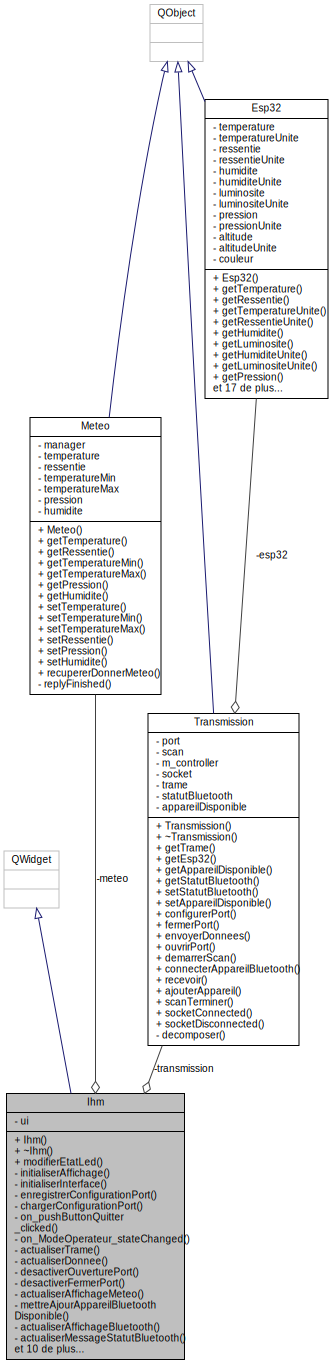
\includegraphics[height=550pt]{class_ihm__coll__graph}
\end{center}
\end{figure}
\subsubsection*{Fonctions membres publiques}
\begin{DoxyCompactItemize}
\item 
\hyperlink{class_ihm_a50a7a15775452923868348bdbe4fa51e}{Ihm} (\hyperlink{class_q_widget}{Q\+Widget} $\ast$parent=nullptr)
\begin{DoxyCompactList}\small\item\em constructeur de la classe \hyperlink{class_ihm}{Ihm} \end{DoxyCompactList}\item 
\hyperlink{class_ihm_add292ea9005bacd1de44dd1ed9ede5b9}{$\sim$\+Ihm} ()
\begin{DoxyCompactList}\small\item\em destructeur de la classe \hyperlink{class_ihm}{Ihm} \end{DoxyCompactList}\item 
void \hyperlink{class_ihm_af0426507c2130aefd01bdb4f825ae168}{modifier\+Etat\+Led} ()
\begin{DoxyCompactList}\small\item\em Méthode qui actualise l\textquotesingle{}etat de la led dans ihm et change le radiobutton activer en fontion de l\textquotesingle{}etat. \end{DoxyCompactList}\end{DoxyCompactItemize}
\subsubsection*{Connecteurs privés}
\begin{DoxyCompactItemize}
\item 
void \hyperlink{class_ihm_ac5c16e4562308547603acc9ef76df570}{on\+\_\+push\+Button\+Quitter\+\_\+clicked} ()
\begin{DoxyCompactList}\small\item\em Méthode appelée lorsque le Bouton quitté est enclenché \end{DoxyCompactList}\item 
void \hyperlink{class_ihm_aeb9414496621bcc42dc63d3ad6e194f9}{on\+\_\+\+Mode\+Operateur\+\_\+state\+Changed} (int arg1)
\begin{DoxyCompactList}\small\item\em Méthode appelée lorsque le case à cocher Mode operateur est enclenché \end{DoxyCompactList}\item 
void \hyperlink{class_ihm_a94ea90d27fc0aa7598cf270dd3be98eb}{actualiser\+Trame} ()
\begin{DoxyCompactList}\small\item\em ajout la nouvelle trame recu dans le mode operateur \end{DoxyCompactList}\item 
void \hyperlink{class_ihm_a7c0a160f30e11a4f8d56b174e07566fe}{actualiser\+Donnee} ()
\item 
void \hyperlink{class_ihm_ab0a18639faa9f2c0b2a141321be4b973}{desactiver\+Ouverture\+Port} ()
\begin{DoxyCompactList}\small\item\em desactive des bouton de l\textquotesingle{}\hyperlink{class_ihm}{Ihm} \end{DoxyCompactList}\item 
void \hyperlink{class_ihm_a6a9bb865ffa3baf686ce16f11f69c57f}{desactiver\+Fermer\+Port} ()
\begin{DoxyCompactList}\small\item\em desactive des bouton de l\textquotesingle{}\hyperlink{class_ihm}{Ihm} \end{DoxyCompactList}\item 
void \hyperlink{class_ihm_a65487c8229375ff72290bed145876737}{actualiser\+Affichage\+Meteo} ()
\begin{DoxyCompactList}\small\item\em fonction qui actualise les différente donné de la météo \end{DoxyCompactList}\item 
void \hyperlink{class_ihm_a9d9ac22e5d73a010bc75a1fcf2e7ddcb}{mettre\+Ajour\+Appareil\+Bluetooth\+Disponible} ()
\begin{DoxyCompactList}\small\item\em fonction qui met a jour les appareil bluetooth disponible \end{DoxyCompactList}\item 
void \hyperlink{class_ihm_a02118154be39cdd3de7fdbdbe396a534}{actualiser\+Affichage\+Bluetooth} ()
\begin{DoxyCompactList}\small\item\em fonction qui actualise l\textquotesingle{}affichage de la parti bluetooth \end{DoxyCompactList}\item 
void \hyperlink{class_ihm_a5d7e6bdacfedc0f0dc4d7b3516454788}{actualiser\+Message\+Statut\+Connecter\+Bluetooth} ()
\begin{DoxyCompactList}\small\item\em fonction qui actualiser dans l\textquotesingle{}ihm le statut de la connexion avec l\textquotesingle{}appareil \end{DoxyCompactList}\item 
void \hyperlink{class_ihm_ad73cc62bafa9c43288f69fbac2b80508}{actualiser\+Message\+Statut\+Deconnecter\+Bluetooth} ()
\begin{DoxyCompactList}\small\item\em met à jour le message de statut pour afficher que l\textquotesingle{}appareil est déconnecter \end{DoxyCompactList}\item 
void \hyperlink{class_ihm_a29b4c5fba871a30f7f2e5fbe08a2087d}{actualiser\+Message\+Statut\+Erreur\+Bluetooth} ()
\begin{DoxyCompactList}\small\item\em met à jour le message de statut pour afficher une erreur \end{DoxyCompactList}\item 
void \hyperlink{class_ihm_a9ce167b94baead6e318bbd0c5254f842}{on\+\_\+push\+Button\+Ouvrir\+Port\+\_\+clicked} ()
\begin{DoxyCompactList}\small\item\em bouton qui ouvre le port serie \end{DoxyCompactList}\item 
void \hyperlink{class_ihm_abcdae03ce7e83266fb9d3e795df8a171}{on\+\_\+push\+Button\+Fermer\+Port\+\_\+clicked} ()
\begin{DoxyCompactList}\small\item\em bouton qui ferme le port serie \end{DoxyCompactList}\item 
void \hyperlink{class_ihm_afd32da9e614eba44bb1d3630b48e6075}{on\+\_\+push\+Button\+Envoyer\+Trame\+\_\+clicked} ()
\begin{DoxyCompactList}\small\item\em recuperer le texte de la line\+Edit dans l\textquotesingle{}onglet operateur pour l\textquotesingle{}envoyer par le port serie \end{DoxyCompactList}\item 
void \hyperlink{class_ihm_a731ee780915cb90a5dfb11f2e02144c9}{on\+\_\+radio\+Button\+Led\+Rouge\+\_\+clicked} ()
\begin{DoxyCompactList}\small\item\em envoit une trame pour allumer la led en rouge \end{DoxyCompactList}\item 
void \hyperlink{class_ihm_afef5bfaa83383427e615d21d9474f466}{on\+\_\+radio\+Button\+Led\+Vert\+\_\+clicked} ()
\begin{DoxyCompactList}\small\item\em envoit une trame pour allumer la led en vert \end{DoxyCompactList}\item 
void \hyperlink{class_ihm_a7e000e198b11fc38a4459f7749561ded}{on\+\_\+radio\+Button\+Led\+Orange\+\_\+clicked} ()
\begin{DoxyCompactList}\small\item\em envoit une trame pour allumer la led en orange \end{DoxyCompactList}\item 
void \hyperlink{class_ihm_a1e328a2e8165bbef347e901f1bc5534d}{on\+\_\+radio\+Button\+Led\+Off\+\_\+clicked} ()
\begin{DoxyCompactList}\small\item\em envoit une trame pour eteindre la led \end{DoxyCompactList}\item 
void \hyperlink{class_ihm_aa943965aa565ec50e00f433100660892}{on\+\_\+push\+Button\+Ville\+\_\+clicked} ()
\begin{DoxyCompactList}\small\item\em fonction qui envoit la ville contenue dans la line edit \end{DoxyCompactList}\item 
void \hyperlink{class_ihm_a277763bdb63ed529aafba7db513cb630}{on\+\_\+push\+Button\+Scan\+\_\+clicked} ()
\begin{DoxyCompactList}\small\item\em fonction appelée quand le bouton scan est cliqué \end{DoxyCompactList}\item 
void \hyperlink{class_ihm_abf61dda1820e5632485de93983c40196}{on\+\_\+push\+Button\+Connexion\+\_\+clicked} ()
\begin{DoxyCompactList}\small\item\em fonction appelée quand le bouton connexion est cliqué \end{DoxyCompactList}\item 
void \hyperlink{class_ihm_ad176c58fb3c583286544f010ac006b66}{on\+\_\+push\+Button\+Deconnexion\+\_\+clicked} ()
\begin{DoxyCompactList}\small\item\em Méthode appelée quand on clique sur le bouton deconnexion elle réactive la possibilité de se connecter en port série. \end{DoxyCompactList}\item 
void \hyperlink{class_ihm_a132bd248057d7278c6841788961b5898}{on\+\_\+push\+Button\+Graphique\+\_\+clicked} ()
\item 
void \hyperlink{class_ihm_a8ee57b456ba85c2667ebf298f06d60c5}{on\+\_\+check\+Box\+Plein\+Ecran\+\_\+state\+Changed} (int arg1)
\item 
void \hyperlink{class_ihm_a3ca276093d65c42a5fc5a87cbca1972a}{actualiser\+Donnee\+Gps} ()
\item 
void \hyperlink{class_ihm_a850d1c97ed5fe5ba3cf3aa85d81872cd}{on\+\_\+push\+Button\+Envoyer\+Coordonnee\+\_\+clicked} ()
\end{DoxyCompactItemize}
\subsubsection*{Fonctions membres privées}
\begin{DoxyCompactItemize}
\item 
void \hyperlink{class_ihm_a9bd8f55d47f658fa5311b7880cc94114}{initialiser\+Affichage} ()
\begin{DoxyCompactList}\small\item\em remet les lcd\+Number a zero quand le port est fermer \end{DoxyCompactList}\item 
void \hyperlink{class_ihm_a3c6fa78360d39cf904dc3a20b0347ddc}{initialiser\+Interface} ()
\begin{DoxyCompactList}\small\item\em initialise l\textquotesingle{}interface utilisateur \end{DoxyCompactList}\item 
void \hyperlink{class_ihm_a05afaf2191aaae673c5ecd14a6d1c921}{enregistrer\+Configuration\+Port} ()
\begin{DoxyCompactList}\small\item\em enregistrer la configuration du port dans un fichier .ini \end{DoxyCompactList}\item 
void \hyperlink{class_ihm_a7341abb08452b21ef2e5c8cb5095d5b0}{charger\+Configuration\+Port} ()
\begin{DoxyCompactList}\small\item\em charger la configuration du port depuis un fichier .ini \end{DoxyCompactList}\item 
void \hyperlink{class_ihm_a3c792f8eeef5216e76cdb9d9e13eb1aa}{desactiver\+Connexion\+Port\+Serie} ()
\begin{DoxyCompactList}\small\item\em active des objet de l\textquotesingle{}interface quand la connexion bluetooth est activer \end{DoxyCompactList}\item 
void \hyperlink{class_ihm_a58ae5ccbff166bcb6723db14a9cf04d9}{activer\+Connexion\+Port\+Serie} ()
\begin{DoxyCompactList}\small\item\em désactive des objet de l\textquotesingle{}interface quand la connexion bluetooth est activer \end{DoxyCompactList}\item 
void \hyperlink{class_ihm_a7ff481c3a05c7d84be2b66552fafd79e}{desactiver\+Connexion\+Bluetooth} ()
\begin{DoxyCompactList}\small\item\em active des objet de l\textquotesingle{}interface quand la connexion bluetooth est activer \end{DoxyCompactList}\item 
void \hyperlink{class_ihm_ac5d166864f1389aa44b0a6784f1977ca}{activer\+Connexion\+Bluetooth} ()
\begin{DoxyCompactList}\small\item\em désactive des objet de l\textquotesingle{}interface quand la connexion bluetooth est activer \end{DoxyCompactList}\item 
void \hyperlink{class_ihm_a4c456231c8af9eab099e9aaadf8a378b}{Activer\+Controle\+Led} ()
\begin{DoxyCompactList}\small\item\em active la possibilité de contrôler les leds \end{DoxyCompactList}\item 
void \hyperlink{class_ihm_a8315a1d902efb0434267778f8144da96}{Desactiver\+Controle\+Led} ()
\begin{DoxyCompactList}\small\item\em Désactiver la possibilité de contrôler les leds. \end{DoxyCompactList}\item 
void \hyperlink{class_ihm_a2ef778196b2eba5b0ab5cb4e066bc3b7}{initialiser\+Connect} ()
\begin{DoxyCompactList}\small\item\em initialise les connects \end{DoxyCompactList}\end{DoxyCompactItemize}
\subsubsection*{Attributs privés}
\begin{DoxyCompactItemize}
\item 
Ui\+::\+Ihm $\ast$ \hyperlink{class_ihm_a0ac5f47856566ceeeca1720109bf70ea}{ui}
\begin{DoxyCompactList}\small\item\em objet \hyperlink{class_ihm}{Ihm} \end{DoxyCompactList}\item 
\hyperlink{class_transmission}{Transmission} $\ast$ \hyperlink{class_ihm_aa8fa25758a4f3e47e07d1d98f6bbab33}{transmission}
\begin{DoxyCompactList}\small\item\em objet transmission \end{DoxyCompactList}\item 
\hyperlink{class_meteo}{Meteo} $\ast$ \hyperlink{class_ihm_af17b420166b2bb1b3e3b1c4b998a2102}{meteo}
\begin{DoxyCompactList}\small\item\em objet meteo \end{DoxyCompactList}\item 
\hyperlink{class_graphique}{Graphique} $\ast$ \hyperlink{class_ihm_a990b3fe0efe66ae9da5e13a5e0a11291}{graphique}
\begin{DoxyCompactList}\small\item\em objet graphique; \end{DoxyCompactList}\item 
Q\+Process $\ast$ \hyperlink{class_ihm_aa1bea3b8f9bad5c19a662a2b455895fb}{proc}
\begin{DoxyCompactList}\small\item\em pointer proc \end{DoxyCompactList}\end{DoxyCompactItemize}


\subsubsection{Documentation des constructeurs et destructeur}
\index{Ihm@{Ihm}!Ihm@{Ihm}}
\index{Ihm@{Ihm}!Ihm@{Ihm}}
\paragraph[{\texorpdfstring{Ihm(\+Q\+Widget $\ast$parent=nullptr)}{Ihm(QWidget *parent=nullptr)}}]{\setlength{\rightskip}{0pt plus 5cm}Ihm\+::\+Ihm (
\begin{DoxyParamCaption}
\item[{{\bf Q\+Widget} $\ast$}]{parent = {\ttfamily nullptr}}
\end{DoxyParamCaption}
)\hspace{0.3cm}{\ttfamily [explicit]}}\hypertarget{class_ihm_a50a7a15775452923868348bdbe4fa51e}{}\label{class_ihm_a50a7a15775452923868348bdbe4fa51e}

\begin{DoxyParams}{Paramètres}
{\em parent} & \\
\hline
\end{DoxyParams}


Références \hyperlink{class_ihm_a990b3fe0efe66ae9da5e13a5e0a11291}{graphique}, \hyperlink{class_ihm_a9bd8f55d47f658fa5311b7880cc94114}{initialiser\+Affichage()}, \hyperlink{class_ihm_a2ef778196b2eba5b0ab5cb4e066bc3b7}{initialiser\+Connect()}, \hyperlink{class_ihm_a3c6fa78360d39cf904dc3a20b0347ddc}{initialiser\+Interface()}, \hyperlink{class_ihm_af17b420166b2bb1b3e3b1c4b998a2102}{meteo}, \hyperlink{class_ihm_aa1bea3b8f9bad5c19a662a2b455895fb}{proc}, \hyperlink{class_ihm_aa8fa25758a4f3e47e07d1d98f6bbab33}{transmission}, et \hyperlink{class_ihm_a0ac5f47856566ceeeca1720109bf70ea}{ui}.


\begin{DoxyCode}
00024                         :
00025     \hyperlink{class_q_widget}{QWidget}(parent),
00026     \hyperlink{class_ihm_a0ac5f47856566ceeeca1720109bf70ea}{ui}(\textcolor{keyword}{new} Ui::Ihm)
00027 \{
00028     \hyperlink{class_ihm_a0ac5f47856566ceeeca1720109bf70ea}{ui}->setupUi(\textcolor{keyword}{this});
00029 
00030     \hyperlink{class_ihm_a3c6fa78360d39cf904dc3a20b0347ddc}{initialiserInterface}();
00031     \hyperlink{class_ihm_a9bd8f55d47f658fa5311b7880cc94114}{initialiserAffichage}();
00032 
00033     \hyperlink{class_ihm_aa8fa25758a4f3e47e07d1d98f6bbab33}{transmission} = \textcolor{keyword}{new} \hyperlink{class_transmission}{Transmission}(\textcolor{keyword}{this});
00034     \hyperlink{class_ihm_af17b420166b2bb1b3e3b1c4b998a2102}{meteo} = \textcolor{keyword}{new} \hyperlink{class_meteo}{Meteo}(\textcolor{keyword}{this});
00035     \hyperlink{class_ihm_a990b3fe0efe66ae9da5e13a5e0a11291}{graphique} = \textcolor{keyword}{new} \hyperlink{class_graphique}{Graphique}();
00036     \hyperlink{class_ihm_aa1bea3b8f9bad5c19a662a2b455895fb}{proc} = \textcolor{keyword}{new} QProcess();
00037 
00038     \hyperlink{class_ihm_a2ef778196b2eba5b0ab5cb4e066bc3b7}{initialiserConnect}();
00039 \}
\end{DoxyCode}
\index{Ihm@{Ihm}!````~Ihm@{$\sim$\+Ihm}}
\index{````~Ihm@{$\sim$\+Ihm}!Ihm@{Ihm}}
\paragraph[{\texorpdfstring{$\sim$\+Ihm()}{~Ihm()}}]{\setlength{\rightskip}{0pt plus 5cm}Ihm\+::$\sim$\+Ihm (
\begin{DoxyParamCaption}
{}
\end{DoxyParamCaption}
)}\hypertarget{class_ihm_add292ea9005bacd1de44dd1ed9ede5b9}{}\label{class_ihm_add292ea9005bacd1de44dd1ed9ede5b9}
constructeur de la classe \hyperlink{class_ihm}{Ihm} 

Références \hyperlink{class_ihm_a05afaf2191aaae673c5ecd14a6d1c921}{enregistrer\+Configuration\+Port()}, \hyperlink{class_ihm_a990b3fe0efe66ae9da5e13a5e0a11291}{graphique}, et \hyperlink{class_ihm_a0ac5f47856566ceeeca1720109bf70ea}{ui}.


\begin{DoxyCode}
00047 \{
00048     \hyperlink{class_ihm_a05afaf2191aaae673c5ecd14a6d1c921}{enregistrerConfigurationPort}();
00049     \textcolor{keyword}{delete} \hyperlink{class_ihm_a990b3fe0efe66ae9da5e13a5e0a11291}{graphique};
00050     \textcolor{keyword}{delete} \hyperlink{class_ihm_a0ac5f47856566ceeeca1720109bf70ea}{ui};
00051 \}
\end{DoxyCode}


\subsubsection{Documentation des fonctions membres}
\index{Ihm@{Ihm}!activer\+Connexion\+Bluetooth@{activer\+Connexion\+Bluetooth}}
\index{activer\+Connexion\+Bluetooth@{activer\+Connexion\+Bluetooth}!Ihm@{Ihm}}
\paragraph[{\texorpdfstring{activer\+Connexion\+Bluetooth()}{activerConnexionBluetooth()}}]{\setlength{\rightskip}{0pt plus 5cm}void Ihm\+::activer\+Connexion\+Bluetooth (
\begin{DoxyParamCaption}
{}
\end{DoxyParamCaption}
)\hspace{0.3cm}{\ttfamily [private]}}\hypertarget{class_ihm_ac5d166864f1389aa44b0a6784f1977ca}{}\label{class_ihm_ac5d166864f1389aa44b0a6784f1977ca}
cette methode et appeler pour desactiver la possibiliter de connexion par bluetooth car une connexion par port serie est en cour 

Références \hyperlink{class_ihm_a0ac5f47856566ceeeca1720109bf70ea}{ui}.


\begin{DoxyCode}
00603 \{
00604     \hyperlink{class_ihm_a0ac5f47856566ceeeca1720109bf70ea}{ui}->comboBoxBluetooth->setDisabled(\textcolor{keyword}{false});
00605     \hyperlink{class_ihm_a0ac5f47856566ceeeca1720109bf70ea}{ui}->pushButtonScan->setDisabled(\textcolor{keyword}{false});
00606     \hyperlink{class_ihm_a0ac5f47856566ceeeca1720109bf70ea}{ui}->pushButtonConnexion->setDisabled(\textcolor{keyword}{false});
00607     \hyperlink{class_ihm_a0ac5f47856566ceeeca1720109bf70ea}{ui}->pushButtonDeconnexion->setDisabled(\textcolor{keyword}{false});
00608     \hyperlink{class_ihm_a0ac5f47856566ceeeca1720109bf70ea}{ui}->labelStatut->setText(\textcolor{stringliteral}{""});
00609 \}
\end{DoxyCode}
\index{Ihm@{Ihm}!activer\+Connexion\+Port\+Serie@{activer\+Connexion\+Port\+Serie}}
\index{activer\+Connexion\+Port\+Serie@{activer\+Connexion\+Port\+Serie}!Ihm@{Ihm}}
\paragraph[{\texorpdfstring{activer\+Connexion\+Port\+Serie()}{activerConnexionPortSerie()}}]{\setlength{\rightskip}{0pt plus 5cm}void Ihm\+::activer\+Connexion\+Port\+Serie (
\begin{DoxyParamCaption}
{}
\end{DoxyParamCaption}
)\hspace{0.3cm}{\ttfamily [private]}}\hypertarget{class_ihm_a58ae5ccbff166bcb6723db14a9cf04d9}{}\label{class_ihm_a58ae5ccbff166bcb6723db14a9cf04d9}
cette methode et appeler pour desactiver la possibiliter de connexion par port serie car une connexion bluetooth est en cour 

Références \hyperlink{class_ihm_a0ac5f47856566ceeeca1720109bf70ea}{ui}.


\begin{DoxyCode}
00574 \{
00575     \hyperlink{class_ihm_a0ac5f47856566ceeeca1720109bf70ea}{ui}->comboBoxAppareil->setDisabled(\textcolor{keyword}{false});
00576     \hyperlink{class_ihm_a0ac5f47856566ceeeca1720109bf70ea}{ui}->comboBoxDebitBaud->setDisabled(\textcolor{keyword}{false});
00577     \hyperlink{class_ihm_a0ac5f47856566ceeeca1720109bf70ea}{ui}->comboBoxBitsDonnees->setDisabled(\textcolor{keyword}{false});
00578     \hyperlink{class_ihm_a0ac5f47856566ceeeca1720109bf70ea}{ui}->comboBoxBitsStop->setDisabled(\textcolor{keyword}{false});
00579     \hyperlink{class_ihm_a0ac5f47856566ceeeca1720109bf70ea}{ui}->pushButtonOuvrirPort->setDisabled(\textcolor{keyword}{false});
00580 \}
\end{DoxyCode}
\index{Ihm@{Ihm}!Activer\+Controle\+Led@{Activer\+Controle\+Led}}
\index{Activer\+Controle\+Led@{Activer\+Controle\+Led}!Ihm@{Ihm}}
\paragraph[{\texorpdfstring{Activer\+Controle\+Led()}{ActiverControleLed()}}]{\setlength{\rightskip}{0pt plus 5cm}void Ihm\+::\+Activer\+Controle\+Led (
\begin{DoxyParamCaption}
{}
\end{DoxyParamCaption}
)\hspace{0.3cm}{\ttfamily [private]}}\hypertarget{class_ihm_a4c456231c8af9eab099e9aaadf8a378b}{}\label{class_ihm_a4c456231c8af9eab099e9aaadf8a378b}
cette methode et appeler pour activer la possibiliter de connexion par bluetooth car aucun connexion en cour 

Références \hyperlink{class_ihm_a0ac5f47856566ceeeca1720109bf70ea}{ui}.



Référencé par \hyperlink{class_ihm_a5d7e6bdacfedc0f0dc4d7b3516454788}{actualiser\+Message\+Statut\+Connecter\+Bluetooth()}, et \hyperlink{class_ihm_ab0a18639faa9f2c0b2a141321be4b973}{desactiver\+Ouverture\+Port()}.


\begin{DoxyCode}
00273 \{
00274     \hyperlink{class_ihm_a0ac5f47856566ceeeca1720109bf70ea}{ui}->radioButtonLedOff->setDisabled(\textcolor{keyword}{false});
00275     \hyperlink{class_ihm_a0ac5f47856566ceeeca1720109bf70ea}{ui}->radioButtonLedVert->setDisabled(\textcolor{keyword}{false});
00276     \hyperlink{class_ihm_a0ac5f47856566ceeeca1720109bf70ea}{ui}->radioButtonLedRouge->setDisabled(\textcolor{keyword}{false});
00277     \hyperlink{class_ihm_a0ac5f47856566ceeeca1720109bf70ea}{ui}->radioButtonLedOrange->setDisabled(\textcolor{keyword}{false});
00278 \}
\end{DoxyCode}
\index{Ihm@{Ihm}!actualiser\+Affichage\+Bluetooth@{actualiser\+Affichage\+Bluetooth}}
\index{actualiser\+Affichage\+Bluetooth@{actualiser\+Affichage\+Bluetooth}!Ihm@{Ihm}}
\paragraph[{\texorpdfstring{actualiser\+Affichage\+Bluetooth}{actualiserAffichageBluetooth}}]{\setlength{\rightskip}{0pt plus 5cm}void Ihm\+::actualiser\+Affichage\+Bluetooth (
\begin{DoxyParamCaption}
{}
\end{DoxyParamCaption}
)\hspace{0.3cm}{\ttfamily [private]}, {\ttfamily [slot]}}\hypertarget{class_ihm_a02118154be39cdd3de7fdbdbe396a534}{}\label{class_ihm_a02118154be39cdd3de7fdbdbe396a534}
methode qui actualiser les appareil disponible 

Références \hyperlink{class_ihm_a0ac5f47856566ceeeca1720109bf70ea}{ui}.



Référencé par \hyperlink{class_ihm_a2ef778196b2eba5b0ab5cb4e066bc3b7}{initialiser\+Connect()}.


\begin{DoxyCode}
00472 \{
00473     \hyperlink{class_ihm_a0ac5f47856566ceeeca1720109bf70ea}{ui}->pushButtonScan->setEnabled(\textcolor{keyword}{true});
00474     \hyperlink{class_ihm_a0ac5f47856566ceeeca1720109bf70ea}{ui}->pushButtonConnexion->setEnabled(\textcolor{keyword}{true});
00475     \hyperlink{class_ihm_a0ac5f47856566ceeeca1720109bf70ea}{ui}->labelStatut->setText(\textcolor{stringliteral}{"<font color=\(\backslash\)"#19B2AD\(\backslash\)">scan terminé</font>"});
00476 \}
\end{DoxyCode}
\index{Ihm@{Ihm}!actualiser\+Affichage\+Meteo@{actualiser\+Affichage\+Meteo}}
\index{actualiser\+Affichage\+Meteo@{actualiser\+Affichage\+Meteo}!Ihm@{Ihm}}
\paragraph[{\texorpdfstring{actualiser\+Affichage\+Meteo}{actualiserAffichageMeteo}}]{\setlength{\rightskip}{0pt plus 5cm}void Ihm\+::actualiser\+Affichage\+Meteo (
\begin{DoxyParamCaption}
{}
\end{DoxyParamCaption}
)\hspace{0.3cm}{\ttfamily [private]}, {\ttfamily [slot]}}\hypertarget{class_ihm_a65487c8229375ff72290bed145876737}{}\label{class_ihm_a65487c8229375ff72290bed145876737}
Méthode appelée quand un port serie et fermer 

Références \hyperlink{class_meteo_a336cfea55c062ebe45fbc7d1a48aaaa1}{Meteo\+::get\+Humidite()}, \hyperlink{class_meteo_a2a4cd85d63157f6b682d37f9c19d1683}{Meteo\+::get\+Pression()}, \hyperlink{class_meteo_a7bcbc6280fb91ff28436e84f7d8765e7}{Meteo\+::get\+Ressentie()}, \hyperlink{class_meteo_ad0a7466f4371df14623fd03fa0bab8dd}{Meteo\+::get\+Temperature()}, \hyperlink{class_meteo_a114aadb20b0b56c1fe8a6fc2dd19c02b}{Meteo\+::get\+Temperature\+Max()}, \hyperlink{class_meteo_a0cef4ff7ae16cfcd820d164d1c5334c4}{Meteo\+::get\+Temperature\+Min()}, \hyperlink{class_meteo_af9ceb3e99e123e6931f8cd9cfde57834}{Meteo\+::get\+Ville()}, \hyperlink{class_ihm_af17b420166b2bb1b3e3b1c4b998a2102}{meteo}, et \hyperlink{class_ihm_a0ac5f47856566ceeeca1720109bf70ea}{ui}.



Référencé par \hyperlink{class_ihm_a2ef778196b2eba5b0ab5cb4e066bc3b7}{initialiser\+Connect()}.


\begin{DoxyCode}
00362 \{
00363     \hyperlink{class_ihm_a0ac5f47856566ceeeca1720109bf70ea}{ui}->lineEditVille->setText(\hyperlink{class_ihm_af17b420166b2bb1b3e3b1c4b998a2102}{meteo}->\hyperlink{class_meteo_af9ceb3e99e123e6931f8cd9cfde57834}{getVille}());
00364     \hyperlink{class_ihm_a0ac5f47856566ceeeca1720109bf70ea}{ui}->lcdNumberTemperatureMeteo->display(\hyperlink{class_ihm_af17b420166b2bb1b3e3b1c4b998a2102}{meteo}->\hyperlink{class_meteo_ad0a7466f4371df14623fd03fa0bab8dd}{getTemperature}());
00365     \hyperlink{class_ihm_a0ac5f47856566ceeeca1720109bf70ea}{ui}->lcdNumberHumiditeMeteo->display(\hyperlink{class_ihm_af17b420166b2bb1b3e3b1c4b998a2102}{meteo}->\hyperlink{class_meteo_a336cfea55c062ebe45fbc7d1a48aaaa1}{getHumidite}());
00366     \hyperlink{class_ihm_a0ac5f47856566ceeeca1720109bf70ea}{ui}->lcdNumberRessentieMeteo->display(\hyperlink{class_ihm_af17b420166b2bb1b3e3b1c4b998a2102}{meteo}->\hyperlink{class_meteo_a7bcbc6280fb91ff28436e84f7d8765e7}{getRessentie}());
00367     \hyperlink{class_ihm_a0ac5f47856566ceeeca1720109bf70ea}{ui}->lcdNumberPressionMeteo->display(\hyperlink{class_ihm_af17b420166b2bb1b3e3b1c4b998a2102}{meteo}->\hyperlink{class_meteo_a2a4cd85d63157f6b682d37f9c19d1683}{getPression}());
00368     \hyperlink{class_ihm_a0ac5f47856566ceeeca1720109bf70ea}{ui}->lcdNumberTempMinMeteo->display(\hyperlink{class_ihm_af17b420166b2bb1b3e3b1c4b998a2102}{meteo}->\hyperlink{class_meteo_a0cef4ff7ae16cfcd820d164d1c5334c4}{getTemperatureMin}());
00369     \hyperlink{class_ihm_a0ac5f47856566ceeeca1720109bf70ea}{ui}->lcdNumberTempMaxMeteo->display(\hyperlink{class_ihm_af17b420166b2bb1b3e3b1c4b998a2102}{meteo}->\hyperlink{class_meteo_a114aadb20b0b56c1fe8a6fc2dd19c02b}{getTemperatureMax}());
00370 \}
\end{DoxyCode}
\index{Ihm@{Ihm}!actualiser\+Donnee@{actualiser\+Donnee}}
\index{actualiser\+Donnee@{actualiser\+Donnee}!Ihm@{Ihm}}
\paragraph[{\texorpdfstring{actualiser\+Donnee}{actualiserDonnee}}]{\setlength{\rightskip}{0pt plus 5cm}void Ihm\+::actualiser\+Donnee (
\begin{DoxyParamCaption}
{}
\end{DoxyParamCaption}
)\hspace{0.3cm}{\ttfamily [private]}, {\ttfamily [slot]}}\hypertarget{class_ihm_a7c0a160f30e11a4f8d56b174e07566fe}{}\label{class_ihm_a7c0a160f30e11a4f8d56b174e07566fe}
met a jour l\textquotesingle{}affichage de la trame en mode operateur lors du signal trame\+Recue() 

Références \hyperlink{class_graphique_ad3dd36f05a9923054a0a2138f96f0311}{Graphique\+::ajouter\+Donnee\+Humidite()}, \hyperlink{class_graphique_a1af0e1968998cb7b5ee8add1197cb0e0}{Graphique\+::ajouter\+Donnee\+Luminosite()}, \hyperlink{class_graphique_a289f0631e56465012511fd7ec9da1b23}{Graphique\+::ajouter\+Donnee\+Pression()}, \hyperlink{class_graphique_a42b3c986ca86c426adbb8fdb03a04380}{Graphique\+::ajouter\+Donnee\+Temperature()}, \hyperlink{class_esp32_a31b691e6c75c1f9859bde4c0df8fe12f}{Esp32\+::get\+Altitude()}, \hyperlink{class_esp32_aad3c2e4b5d15a02abc62d0329f43942d}{Esp32\+::get\+Altitude\+Unite()}, \hyperlink{class_transmission_afccd88f8be8c204a0960bc2d6970931f}{Transmission\+::get\+Esp32()}, \hyperlink{class_esp32_a87f581ef8f01bcb71a7294cc545b242e}{Esp32\+::get\+Humidite()}, \hyperlink{class_esp32_ab2a1fc92c11af031814569f3d2836f33}{Esp32\+::get\+Humidite\+Unite()}, \hyperlink{class_esp32_aa2cdabace1ce70928c53d25e306a16d1}{Esp32\+::get\+Luminosite()}, \hyperlink{class_esp32_a50f4ef373379d2dbc0fd960438ab6f93}{Esp32\+::get\+Luminosite\+Unite()}, \hyperlink{class_esp32_a31155a36108b37febae371d9ae65385a}{Esp32\+::get\+Pression()}, \hyperlink{class_esp32_a398d4a1cbc61f7af2f3af7ecbcf2f93f}{Esp32\+::get\+Pression\+Unite()}, \hyperlink{class_esp32_ae29854a5127d760a216f96ec7d797412}{Esp32\+::get\+Ressentie()}, \hyperlink{class_esp32_a548ed7533f742d087c65df256479ed00}{Esp32\+::get\+Ressentie\+Unite()}, \hyperlink{class_esp32_adb339413686f3d78df1ecd41f106fd4e}{Esp32\+::get\+Temperature()}, \hyperlink{class_esp32_ae20c976b79f87de083ca8ee49b2abf25}{Esp32\+::get\+Temperature\+Unite()}, \hyperlink{class_ihm_a990b3fe0efe66ae9da5e13a5e0a11291}{graphique}, \hyperlink{class_ihm_af0426507c2130aefd01bdb4f825ae168}{modifier\+Etat\+Led()}, \hyperlink{class_ihm_aa8fa25758a4f3e47e07d1d98f6bbab33}{transmission}, et \hyperlink{class_ihm_a0ac5f47856566ceeeca1720109bf70ea}{ui}.



Référencé par \hyperlink{class_ihm_a2ef778196b2eba5b0ab5cb4e066bc3b7}{initialiser\+Connect()}.


\begin{DoxyCode}
00219 \{
00220     QDateTime maintenant = QDateTime::currentDateTime();
00221     QString heure = maintenant.toString(\textcolor{stringliteral}{"hh:mm:ss"});
00222     \hyperlink{class_ihm_a0ac5f47856566ceeeca1720109bf70ea}{ui}->horodatage->setText(heure);
00223 
00224     \hyperlink{class_ihm_a0ac5f47856566ceeeca1720109bf70ea}{ui}->lcdNumberTemperature->display(\hyperlink{class_ihm_aa8fa25758a4f3e47e07d1d98f6bbab33}{transmission}->\hyperlink{class_transmission_afccd88f8be8c204a0960bc2d6970931f}{getEsp32}()->
      \hyperlink{class_esp32_adb339413686f3d78df1ecd41f106fd4e}{getTemperature}());
00225     \hyperlink{class_ihm_a0ac5f47856566ceeeca1720109bf70ea}{ui}->lcdNumberHumidite->display(\hyperlink{class_ihm_aa8fa25758a4f3e47e07d1d98f6bbab33}{transmission}->\hyperlink{class_transmission_afccd88f8be8c204a0960bc2d6970931f}{getEsp32}()->
      \hyperlink{class_esp32_a87f581ef8f01bcb71a7294cc545b242e}{getHumidite}());
00226     \hyperlink{class_ihm_a0ac5f47856566ceeeca1720109bf70ea}{ui}->lcdNumberRessentie->display(\hyperlink{class_ihm_aa8fa25758a4f3e47e07d1d98f6bbab33}{transmission}->\hyperlink{class_transmission_afccd88f8be8c204a0960bc2d6970931f}{getEsp32}()->
      \hyperlink{class_esp32_ae29854a5127d760a216f96ec7d797412}{getRessentie}());
00227     \hyperlink{class_ihm_a0ac5f47856566ceeeca1720109bf70ea}{ui}->lcdNumberLuminosite->display(\hyperlink{class_ihm_aa8fa25758a4f3e47e07d1d98f6bbab33}{transmission}->\hyperlink{class_transmission_afccd88f8be8c204a0960bc2d6970931f}{getEsp32}()->
      \hyperlink{class_esp32_aa2cdabace1ce70928c53d25e306a16d1}{getLuminosite}());
00228     \hyperlink{class_ihm_a0ac5f47856566ceeeca1720109bf70ea}{ui}->lcdNumberPression->display(\hyperlink{class_ihm_aa8fa25758a4f3e47e07d1d98f6bbab33}{transmission}->\hyperlink{class_transmission_afccd88f8be8c204a0960bc2d6970931f}{getEsp32}()->
      \hyperlink{class_esp32_a31155a36108b37febae371d9ae65385a}{getPression}());
00229     \hyperlink{class_ihm_a0ac5f47856566ceeeca1720109bf70ea}{ui}->lcdNumberAltitude->display(\hyperlink{class_ihm_aa8fa25758a4f3e47e07d1d98f6bbab33}{transmission}->\hyperlink{class_transmission_afccd88f8be8c204a0960bc2d6970931f}{getEsp32}()->
      \hyperlink{class_esp32_a31b691e6c75c1f9859bde4c0df8fe12f}{getAltitude}());
00230 
00231     \hyperlink{class_ihm_a0ac5f47856566ceeeca1720109bf70ea}{ui}->labelUniteTemperature->setText(\hyperlink{class_ihm_aa8fa25758a4f3e47e07d1d98f6bbab33}{transmission}->\hyperlink{class_transmission_afccd88f8be8c204a0960bc2d6970931f}{getEsp32}()->
      \hyperlink{class_esp32_ae20c976b79f87de083ca8ee49b2abf25}{getTemperatureUnite}());
00232     \hyperlink{class_ihm_a0ac5f47856566ceeeca1720109bf70ea}{ui}->labelUniteRessenti->setText(\hyperlink{class_ihm_aa8fa25758a4f3e47e07d1d98f6bbab33}{transmission}->\hyperlink{class_transmission_afccd88f8be8c204a0960bc2d6970931f}{getEsp32}()->
      \hyperlink{class_esp32_a548ed7533f742d087c65df256479ed00}{getRessentieUnite}());
00233     \hyperlink{class_ihm_a0ac5f47856566ceeeca1720109bf70ea}{ui}->labelUniteHumidite->setText(\hyperlink{class_ihm_aa8fa25758a4f3e47e07d1d98f6bbab33}{transmission}->\hyperlink{class_transmission_afccd88f8be8c204a0960bc2d6970931f}{getEsp32}()->
      \hyperlink{class_esp32_ab2a1fc92c11af031814569f3d2836f33}{getHumiditeUnite}());
00234     \hyperlink{class_ihm_a0ac5f47856566ceeeca1720109bf70ea}{ui}->labelUniteLuminosite->setText(\hyperlink{class_ihm_aa8fa25758a4f3e47e07d1d98f6bbab33}{transmission}->\hyperlink{class_transmission_afccd88f8be8c204a0960bc2d6970931f}{getEsp32}()->
      \hyperlink{class_esp32_a50f4ef373379d2dbc0fd960438ab6f93}{getLuminositeUnite}());
00235     \hyperlink{class_ihm_a0ac5f47856566ceeeca1720109bf70ea}{ui}->labelUnitePression->setText(\hyperlink{class_ihm_aa8fa25758a4f3e47e07d1d98f6bbab33}{transmission}->\hyperlink{class_transmission_afccd88f8be8c204a0960bc2d6970931f}{getEsp32}()->
      \hyperlink{class_esp32_a398d4a1cbc61f7af2f3af7ecbcf2f93f}{getPressionUnite}());
00236     \hyperlink{class_ihm_a0ac5f47856566ceeeca1720109bf70ea}{ui}->labelUniteAltitude->setText(\hyperlink{class_ihm_aa8fa25758a4f3e47e07d1d98f6bbab33}{transmission}->\hyperlink{class_transmission_afccd88f8be8c204a0960bc2d6970931f}{getEsp32}()->
      \hyperlink{class_esp32_aad3c2e4b5d15a02abc62d0329f43942d}{getAltitudeUnite}());
00237 
00238     \hyperlink{class_ihm_af0426507c2130aefd01bdb4f825ae168}{modifierEtatLed}();
00239 
00240     \hyperlink{class_ihm_a990b3fe0efe66ae9da5e13a5e0a11291}{graphique}->\hyperlink{class_graphique_a42b3c986ca86c426adbb8fdb03a04380}{ajouterDonneeTemperature}(
      \hyperlink{class_ihm_aa8fa25758a4f3e47e07d1d98f6bbab33}{transmission}->\hyperlink{class_transmission_afccd88f8be8c204a0960bc2d6970931f}{getEsp32}()->\hyperlink{class_esp32_adb339413686f3d78df1ecd41f106fd4e}{getTemperature}());
00241     \hyperlink{class_ihm_a990b3fe0efe66ae9da5e13a5e0a11291}{graphique}->\hyperlink{class_graphique_ad3dd36f05a9923054a0a2138f96f0311}{ajouterDonneeHumidite}(\hyperlink{class_ihm_aa8fa25758a4f3e47e07d1d98f6bbab33}{transmission}->
      \hyperlink{class_transmission_afccd88f8be8c204a0960bc2d6970931f}{getEsp32}()->\hyperlink{class_esp32_a87f581ef8f01bcb71a7294cc545b242e}{getHumidite}());
00242     \hyperlink{class_ihm_a990b3fe0efe66ae9da5e13a5e0a11291}{graphique}->\hyperlink{class_graphique_a1af0e1968998cb7b5ee8add1197cb0e0}{ajouterDonneeLuminosite}(
      \hyperlink{class_ihm_aa8fa25758a4f3e47e07d1d98f6bbab33}{transmission}->\hyperlink{class_transmission_afccd88f8be8c204a0960bc2d6970931f}{getEsp32}()->\hyperlink{class_esp32_aa2cdabace1ce70928c53d25e306a16d1}{getLuminosite}());
00243     \hyperlink{class_ihm_a990b3fe0efe66ae9da5e13a5e0a11291}{graphique}->\hyperlink{class_graphique_a289f0631e56465012511fd7ec9da1b23}{ajouterDonneePression}(\hyperlink{class_ihm_aa8fa25758a4f3e47e07d1d98f6bbab33}{transmission}->
      \hyperlink{class_transmission_afccd88f8be8c204a0960bc2d6970931f}{getEsp32}()->\hyperlink{class_esp32_a31155a36108b37febae371d9ae65385a}{getPression}());
00244 \}
\end{DoxyCode}
\index{Ihm@{Ihm}!actualiser\+Donnee\+Gps@{actualiser\+Donnee\+Gps}}
\index{actualiser\+Donnee\+Gps@{actualiser\+Donnee\+Gps}!Ihm@{Ihm}}
\paragraph[{\texorpdfstring{actualiser\+Donnee\+Gps}{actualiserDonneeGps}}]{\setlength{\rightskip}{0pt plus 5cm}void Ihm\+::actualiser\+Donnee\+Gps (
\begin{DoxyParamCaption}
{}
\end{DoxyParamCaption}
)\hspace{0.3cm}{\ttfamily [private]}, {\ttfamily [slot]}}\hypertarget{class_ihm_a3ca276093d65c42a5fc5a87cbca1972a}{}\label{class_ihm_a3ca276093d65c42a5fc5a87cbca1972a}
Méthode appelée dès que l\textquotesingle{}etat du check\+Box plein ecran change 

Références \hyperlink{class_transmission_aa5004c178152de5b94ef14e11e80792c}{Transmission\+::get\+Gps()}, \hyperlink{class_gps_a44c6469bf67727853c06d4be037c6b0f}{Gps\+::get\+Latitude()}, \hyperlink{class_gps_a6ce8da770e213bfbf7f204b107d9e3f5}{Gps\+::get\+Longitude()}, \hyperlink{class_ihm_aa8fa25758a4f3e47e07d1d98f6bbab33}{transmission}, et \hyperlink{class_ihm_a0ac5f47856566ceeeca1720109bf70ea}{ui}.



Référencé par \hyperlink{class_ihm_a2ef778196b2eba5b0ab5cb4e066bc3b7}{initialiser\+Connect()}.


\begin{DoxyCode}
00645 \{
00646     \hyperlink{class_ihm_a0ac5f47856566ceeeca1720109bf70ea}{ui}->labelValeurCoordonnee->setText(QString::number(\hyperlink{class_ihm_aa8fa25758a4f3e47e07d1d98f6bbab33}{transmission}->
      \hyperlink{class_transmission_aa5004c178152de5b94ef14e11e80792c}{getGps}()->\hyperlink{class_gps_a44c6469bf67727853c06d4be037c6b0f}{getLatitude}()) + \textcolor{stringliteral}{" "} + QString::number(\hyperlink{class_ihm_aa8fa25758a4f3e47e07d1d98f6bbab33}{transmission}->
      \hyperlink{class_transmission_aa5004c178152de5b94ef14e11e80792c}{getGps}()->\hyperlink{class_gps_a6ce8da770e213bfbf7f204b107d9e3f5}{getLongitude}()));
00647     \hyperlink{class_ihm_a0ac5f47856566ceeeca1720109bf70ea}{ui}->pushButtonEnvoyerCoordonnee->setEnabled(\textcolor{keyword}{true});
00648 \}
\end{DoxyCode}
\index{Ihm@{Ihm}!actualiser\+Message\+Statut\+Connecter\+Bluetooth@{actualiser\+Message\+Statut\+Connecter\+Bluetooth}}
\index{actualiser\+Message\+Statut\+Connecter\+Bluetooth@{actualiser\+Message\+Statut\+Connecter\+Bluetooth}!Ihm@{Ihm}}
\paragraph[{\texorpdfstring{actualiser\+Message\+Statut\+Connecter\+Bluetooth}{actualiserMessageStatutConnecterBluetooth}}]{\setlength{\rightskip}{0pt plus 5cm}void Ihm\+::actualiser\+Message\+Statut\+Connecter\+Bluetooth (
\begin{DoxyParamCaption}
{}
\end{DoxyParamCaption}
)\hspace{0.3cm}{\ttfamily [private]}, {\ttfamily [slot]}}\hypertarget{class_ihm_a5d7e6bdacfedc0f0dc4d7b3516454788}{}\label{class_ihm_a5d7e6bdacfedc0f0dc4d7b3516454788}
methode qui met à jour l\textquotesingle{}affichage des bouton(enable / disable) 

Références \hyperlink{class_ihm_a4c456231c8af9eab099e9aaadf8a378b}{Activer\+Controle\+Led()}, \hyperlink{class_transmission_adf65c6a49fbbc9d25b7b2fca2c410f99}{Transmission\+::get\+Statut\+Bluetooth()}, \hyperlink{class_ihm_aa1bea3b8f9bad5c19a662a2b455895fb}{proc}, \hyperlink{class_ihm_aa8fa25758a4f3e47e07d1d98f6bbab33}{transmission}, et \hyperlink{class_ihm_a0ac5f47856566ceeeca1720109bf70ea}{ui}.



Référencé par \hyperlink{class_ihm_a2ef778196b2eba5b0ab5cb4e066bc3b7}{initialiser\+Connect()}.


\begin{DoxyCode}
00498 \{
00499     \hyperlink{class_ihm_a0ac5f47856566ceeeca1720109bf70ea}{ui}->labelStatut->setText(\textcolor{stringliteral}{"<font color=\(\backslash\)"#f39c12\(\backslash\)">"} + \hyperlink{class_ihm_aa8fa25758a4f3e47e07d1d98f6bbab33}{transmission}->
      \hyperlink{class_transmission_adf65c6a49fbbc9d25b7b2fca2c410f99}{getStatutBluetooth}() + \textcolor{stringliteral}{"</font>"});
00500 
00501     \hyperlink{class_ihm_aa1bea3b8f9bad5c19a662a2b455895fb}{proc}->execute(\textcolor{stringliteral}{"notify-send --icon=/usr/share/icons/hicolor/48x48/apps/bluetooth.png \(\backslash\)""} + 
      \hyperlink{class_ihm_aa8fa25758a4f3e47e07d1d98f6bbab33}{transmission}->\hyperlink{class_transmission_adf65c6a49fbbc9d25b7b2fca2c410f99}{getStatutBluetooth}() + \textcolor{stringliteral}{"\(\backslash\)" "});
00502 
00503     \hyperlink{class_ihm_a0ac5f47856566ceeeca1720109bf70ea}{ui}->pushButtonConnexion->setEnabled(\textcolor{keyword}{false});
00504     \hyperlink{class_ihm_a0ac5f47856566ceeeca1720109bf70ea}{ui}->pushButtonScan->setEnabled(\textcolor{keyword}{false});
00505     \hyperlink{class_ihm_a0ac5f47856566ceeeca1720109bf70ea}{ui}->pushButtonDeconnexion->setEnabled(\textcolor{keyword}{true});
00506     \hyperlink{class_ihm_a0ac5f47856566ceeeca1720109bf70ea}{ui}->lineEditEnvoyerTrame->setDisabled(\textcolor{keyword}{false});
00507     \hyperlink{class_ihm_a0ac5f47856566ceeeca1720109bf70ea}{ui}->pushButtonEnvoyerTrame->setDisabled(\textcolor{keyword}{false});
00508     \textcolor{comment}{//desactiverConnexionPortSerie();}
00509     \hyperlink{class_ihm_a4c456231c8af9eab099e9aaadf8a378b}{ActiverControleLed}();
00510 \}
\end{DoxyCode}
\index{Ihm@{Ihm}!actualiser\+Message\+Statut\+Deconnecter\+Bluetooth@{actualiser\+Message\+Statut\+Deconnecter\+Bluetooth}}
\index{actualiser\+Message\+Statut\+Deconnecter\+Bluetooth@{actualiser\+Message\+Statut\+Deconnecter\+Bluetooth}!Ihm@{Ihm}}
\paragraph[{\texorpdfstring{actualiser\+Message\+Statut\+Deconnecter\+Bluetooth}{actualiserMessageStatutDeconnecterBluetooth}}]{\setlength{\rightskip}{0pt plus 5cm}void Ihm\+::actualiser\+Message\+Statut\+Deconnecter\+Bluetooth (
\begin{DoxyParamCaption}
{}
\end{DoxyParamCaption}
)\hspace{0.3cm}{\ttfamily [private]}, {\ttfamily [slot]}}\hypertarget{class_ihm_ad73cc62bafa9c43288f69fbac2b80508}{}\label{class_ihm_ad73cc62bafa9c43288f69fbac2b80508}
methode qui met à jour le message de statut de la connexion bluetooth (appareil connecter) 

Références \hyperlink{class_ihm_a8315a1d902efb0434267778f8144da96}{Desactiver\+Controle\+Led()}, \hyperlink{class_transmission_adf65c6a49fbbc9d25b7b2fca2c410f99}{Transmission\+::get\+Statut\+Bluetooth()}, \hyperlink{class_ihm_a9bd8f55d47f658fa5311b7880cc94114}{initialiser\+Affichage()}, \hyperlink{class_ihm_aa1bea3b8f9bad5c19a662a2b455895fb}{proc}, \hyperlink{class_ihm_aa8fa25758a4f3e47e07d1d98f6bbab33}{transmission}, et \hyperlink{class_ihm_a0ac5f47856566ceeeca1720109bf70ea}{ui}.



Référencé par \hyperlink{class_ihm_a2ef778196b2eba5b0ab5cb4e066bc3b7}{initialiser\+Connect()}.


\begin{DoxyCode}
00518 \{
00519     \hyperlink{class_ihm_a0ac5f47856566ceeeca1720109bf70ea}{ui}->labelStatut->setText(\textcolor{stringliteral}{"<font color=\(\backslash\)"#7329b9\(\backslash\)">"} + \hyperlink{class_ihm_aa8fa25758a4f3e47e07d1d98f6bbab33}{transmission}->
      \hyperlink{class_transmission_adf65c6a49fbbc9d25b7b2fca2c410f99}{getStatutBluetooth}() + \textcolor{stringliteral}{"</font>"});
00520 
00521     \hyperlink{class_ihm_aa1bea3b8f9bad5c19a662a2b455895fb}{proc}->execute(\textcolor{stringliteral}{"notify-send --icon=/usr/share/icons/hicolor/48x48/apps/bluetooth.png \(\backslash\)""} + 
      \hyperlink{class_ihm_aa8fa25758a4f3e47e07d1d98f6bbab33}{transmission}->\hyperlink{class_transmission_adf65c6a49fbbc9d25b7b2fca2c410f99}{getStatutBluetooth}() + \textcolor{stringliteral}{"\(\backslash\)" "});
00522 
00523     \hyperlink{class_ihm_a0ac5f47856566ceeeca1720109bf70ea}{ui}->pushButtonConnexion->setEnabled(\textcolor{keyword}{true});
00524     \hyperlink{class_ihm_a0ac5f47856566ceeeca1720109bf70ea}{ui}->pushButtonScan->setEnabled(\textcolor{keyword}{true});
00525     \hyperlink{class_ihm_a0ac5f47856566ceeeca1720109bf70ea}{ui}->pushButtonDeconnexion->setEnabled(\textcolor{keyword}{false});
00526     \hyperlink{class_ihm_a0ac5f47856566ceeeca1720109bf70ea}{ui}->lineEditEnvoyerTrame->setDisabled(\textcolor{keyword}{true});
00527     \hyperlink{class_ihm_a0ac5f47856566ceeeca1720109bf70ea}{ui}->pushButtonEnvoyerTrame->setDisabled(\textcolor{keyword}{true});
00528     \hyperlink{class_ihm_a9bd8f55d47f658fa5311b7880cc94114}{initialiserAffichage}();
00529     \hyperlink{class_ihm_a8315a1d902efb0434267778f8144da96}{DesactiverControleLed}();
00530 \}
\end{DoxyCode}
\index{Ihm@{Ihm}!actualiser\+Message\+Statut\+Erreur\+Bluetooth@{actualiser\+Message\+Statut\+Erreur\+Bluetooth}}
\index{actualiser\+Message\+Statut\+Erreur\+Bluetooth@{actualiser\+Message\+Statut\+Erreur\+Bluetooth}!Ihm@{Ihm}}
\paragraph[{\texorpdfstring{actualiser\+Message\+Statut\+Erreur\+Bluetooth}{actualiserMessageStatutErreurBluetooth}}]{\setlength{\rightskip}{0pt plus 5cm}void Ihm\+::actualiser\+Message\+Statut\+Erreur\+Bluetooth (
\begin{DoxyParamCaption}
{}
\end{DoxyParamCaption}
)\hspace{0.3cm}{\ttfamily [private]}, {\ttfamily [slot]}}\hypertarget{class_ihm_a29b4c5fba871a30f7f2e5fbe08a2087d}{}\label{class_ihm_a29b4c5fba871a30f7f2e5fbe08a2087d}
methode qui met à jour le message de statut de la connexion bluetooth (appareil deconnecter) 

Références \hyperlink{class_transmission_adf65c6a49fbbc9d25b7b2fca2c410f99}{Transmission\+::get\+Statut\+Bluetooth()}, \hyperlink{class_ihm_aa8fa25758a4f3e47e07d1d98f6bbab33}{transmission}, et \hyperlink{class_ihm_a0ac5f47856566ceeeca1720109bf70ea}{ui}.



Référencé par \hyperlink{class_ihm_a2ef778196b2eba5b0ab5cb4e066bc3b7}{initialiser\+Connect()}.


\begin{DoxyCode}
00538 \{
00539     \hyperlink{class_ihm_a0ac5f47856566ceeeca1720109bf70ea}{ui}->labelStatut->setText(\textcolor{stringliteral}{"<font color=\(\backslash\)"#7329b9\(\backslash\)">"} + \hyperlink{class_ihm_aa8fa25758a4f3e47e07d1d98f6bbab33}{transmission}->
      \hyperlink{class_transmission_adf65c6a49fbbc9d25b7b2fca2c410f99}{getStatutBluetooth}() + \textcolor{stringliteral}{"</font>"});
00540 \}
\end{DoxyCode}
\index{Ihm@{Ihm}!actualiser\+Trame@{actualiser\+Trame}}
\index{actualiser\+Trame@{actualiser\+Trame}!Ihm@{Ihm}}
\paragraph[{\texorpdfstring{actualiser\+Trame}{actualiserTrame}}]{\setlength{\rightskip}{0pt plus 5cm}void Ihm\+::actualiser\+Trame (
\begin{DoxyParamCaption}
{}
\end{DoxyParamCaption}
)\hspace{0.3cm}{\ttfamily [private]}, {\ttfamily [slot]}}\hypertarget{class_ihm_a94ea90d27fc0aa7598cf270dd3be98eb}{}\label{class_ihm_a94ea90d27fc0aa7598cf270dd3be98eb}
permet de passer en mode Operateur 

Références \hyperlink{class_transmission_a3fc179158c8c9e2cceba36423ef92505}{Transmission\+::get\+Trame()}, \hyperlink{class_ihm_aa8fa25758a4f3e47e07d1d98f6bbab33}{transmission}, et \hyperlink{class_ihm_a0ac5f47856566ceeeca1720109bf70ea}{ui}.



Référencé par \hyperlink{class_ihm_a2ef778196b2eba5b0ab5cb4e066bc3b7}{initialiser\+Connect()}.


\begin{DoxyCode}
00173 \{
00174     QDateTime maintenant = QDateTime::currentDateTime();
00175     QString heure = maintenant.toString(\textcolor{stringliteral}{"hh:mm:ss"});
00176 
00177     \hyperlink{class_ihm_a0ac5f47856566ceeeca1720109bf70ea}{ui}->textEditTrame->setTextColor(Qt::red);
00178     \hyperlink{class_ihm_a0ac5f47856566ceeeca1720109bf70ea}{ui}->textEditTrame->append(heure + \textcolor{stringliteral}{" :"});
00179     \hyperlink{class_ihm_a0ac5f47856566ceeeca1720109bf70ea}{ui}->textEditTrame->setTextColor(Qt::black);
00180     \hyperlink{class_ihm_a0ac5f47856566ceeeca1720109bf70ea}{ui}->textEditTrame->append(\hyperlink{class_ihm_aa8fa25758a4f3e47e07d1d98f6bbab33}{transmission}->\hyperlink{class_transmission_a3fc179158c8c9e2cceba36423ef92505}{getTrame}());
00181 \}
\end{DoxyCode}
\index{Ihm@{Ihm}!charger\+Configuration\+Port@{charger\+Configuration\+Port}}
\index{charger\+Configuration\+Port@{charger\+Configuration\+Port}!Ihm@{Ihm}}
\paragraph[{\texorpdfstring{charger\+Configuration\+Port()}{chargerConfigurationPort()}}]{\setlength{\rightskip}{0pt plus 5cm}void Ihm\+::charger\+Configuration\+Port (
\begin{DoxyParamCaption}
{}
\end{DoxyParamCaption}
)\hspace{0.3cm}{\ttfamily [private]}}\hypertarget{class_ihm_a7341abb08452b21ef2e5c8cb5095d5b0}{}\label{class_ihm_a7341abb08452b21ef2e5c8cb5095d5b0}
cette methode et appeler pour enregistrer la configuration du port dans un fichier .ini 

Références \hyperlink{class_ihm_a0ac5f47856566ceeeca1720109bf70ea}{ui}.



Référencé par \hyperlink{class_ihm_a3c6fa78360d39cf904dc3a20b0347ddc}{initialiser\+Interface()}.


\begin{DoxyCode}
00098 \{
00099     QSettings configuration(\textcolor{stringliteral}{"Sonde.ini"}, QSettings::IniFormat);
00100 
00101     \hyperlink{class_ihm_a0ac5f47856566ceeeca1720109bf70ea}{ui}->comboBoxAppareil->setCurrentText(configuration.value(\textcolor{stringliteral}{"PortSerie/Appareil"},\textcolor{stringliteral}{"/dev/ttyUSB0"}).
      toString());
00102     \hyperlink{class_ihm_a0ac5f47856566ceeeca1720109bf70ea}{ui}->comboBoxDebitBaud->setCurrentText(configuration.value(\textcolor{stringliteral}{"PortSerie/DebitBauds"},\textcolor{stringliteral}{"1200"}).toString());
00103     \hyperlink{class_ihm_a0ac5f47856566ceeeca1720109bf70ea}{ui}->comboBoxBitsDonnees->setCurrentText(configuration.value(\textcolor{stringliteral}{"PortSerie/BitsDonnee"},\textcolor{stringliteral}{"5"}).toString());
00104     \hyperlink{class_ihm_a0ac5f47856566ceeeca1720109bf70ea}{ui}->comboBoxBitsStop->setCurrentText(configuration.value(\textcolor{stringliteral}{"PortSerie/BitsStop"},\textcolor{stringliteral}{"1"}).toString());
00105 \}
\end{DoxyCode}
\index{Ihm@{Ihm}!desactiver\+Connexion\+Bluetooth@{desactiver\+Connexion\+Bluetooth}}
\index{desactiver\+Connexion\+Bluetooth@{desactiver\+Connexion\+Bluetooth}!Ihm@{Ihm}}
\paragraph[{\texorpdfstring{desactiver\+Connexion\+Bluetooth()}{desactiverConnexionBluetooth()}}]{\setlength{\rightskip}{0pt plus 5cm}void Ihm\+::desactiver\+Connexion\+Bluetooth (
\begin{DoxyParamCaption}
{}
\end{DoxyParamCaption}
)\hspace{0.3cm}{\ttfamily [private]}}\hypertarget{class_ihm_a7ff481c3a05c7d84be2b66552fafd79e}{}\label{class_ihm_a7ff481c3a05c7d84be2b66552fafd79e}
cette methode et appeler pour activer la possibiliter de connexion par port serie car aucun connexion en cour 

Références \hyperlink{class_ihm_a0ac5f47856566ceeeca1720109bf70ea}{ui}.


\begin{DoxyCode}
00588 \{
00589     \hyperlink{class_ihm_a0ac5f47856566ceeeca1720109bf70ea}{ui}->comboBoxBluetooth->setDisabled(\textcolor{keyword}{true});
00590     \hyperlink{class_ihm_a0ac5f47856566ceeeca1720109bf70ea}{ui}->pushButtonScan->setDisabled(\textcolor{keyword}{true});
00591     \hyperlink{class_ihm_a0ac5f47856566ceeeca1720109bf70ea}{ui}->pushButtonConnexion->setDisabled(\textcolor{keyword}{true});
00592     \hyperlink{class_ihm_a0ac5f47856566ceeeca1720109bf70ea}{ui}->pushButtonDeconnexion->setDisabled(\textcolor{keyword}{true});
00593     \hyperlink{class_ihm_a0ac5f47856566ceeeca1720109bf70ea}{ui}->labelStatut->setText(\textcolor{stringliteral}{"<font color=\(\backslash\)"#63cb23\(\backslash\)">Connexion Serie en cours...</font>"});
00594 
00595 \}
\end{DoxyCode}
\index{Ihm@{Ihm}!desactiver\+Connexion\+Port\+Serie@{desactiver\+Connexion\+Port\+Serie}}
\index{desactiver\+Connexion\+Port\+Serie@{desactiver\+Connexion\+Port\+Serie}!Ihm@{Ihm}}
\paragraph[{\texorpdfstring{desactiver\+Connexion\+Port\+Serie()}{desactiverConnexionPortSerie()}}]{\setlength{\rightskip}{0pt plus 5cm}void Ihm\+::desactiver\+Connexion\+Port\+Serie (
\begin{DoxyParamCaption}
{}
\end{DoxyParamCaption}
)\hspace{0.3cm}{\ttfamily [private]}}\hypertarget{class_ihm_a3c792f8eeef5216e76cdb9d9e13eb1aa}{}\label{class_ihm_a3c792f8eeef5216e76cdb9d9e13eb1aa}
cette methode et appeler pour charger la configuration du port depuis un fichier .ini 

Références \hyperlink{class_ihm_a0ac5f47856566ceeeca1720109bf70ea}{ui}.


\begin{DoxyCode}
00559 \{
00560     \hyperlink{class_ihm_a0ac5f47856566ceeeca1720109bf70ea}{ui}->comboBoxAppareil->setDisabled(\textcolor{keyword}{true});
00561     \hyperlink{class_ihm_a0ac5f47856566ceeeca1720109bf70ea}{ui}->comboBoxDebitBaud->setDisabled(\textcolor{keyword}{true});
00562     \hyperlink{class_ihm_a0ac5f47856566ceeeca1720109bf70ea}{ui}->comboBoxBitsDonnees->setDisabled(\textcolor{keyword}{true});
00563     \hyperlink{class_ihm_a0ac5f47856566ceeeca1720109bf70ea}{ui}->comboBoxBitsStop->setDisabled(\textcolor{keyword}{true});
00564     \hyperlink{class_ihm_a0ac5f47856566ceeeca1720109bf70ea}{ui}->pushButtonOuvrirPort->setDisabled(\textcolor{keyword}{true});
00565     \hyperlink{class_ihm_a0ac5f47856566ceeeca1720109bf70ea}{ui}->pushButtonFermerPort->setDisabled(\textcolor{keyword}{true});
00566 \}
\end{DoxyCode}
\index{Ihm@{Ihm}!Desactiver\+Controle\+Led@{Desactiver\+Controle\+Led}}
\index{Desactiver\+Controle\+Led@{Desactiver\+Controle\+Led}!Ihm@{Ihm}}
\paragraph[{\texorpdfstring{Desactiver\+Controle\+Led()}{DesactiverControleLed()}}]{\setlength{\rightskip}{0pt plus 5cm}void Ihm\+::\+Desactiver\+Controle\+Led (
\begin{DoxyParamCaption}
{}
\end{DoxyParamCaption}
)\hspace{0.3cm}{\ttfamily [private]}}\hypertarget{class_ihm_a8315a1d902efb0434267778f8144da96}{}\label{class_ihm_a8315a1d902efb0434267778f8144da96}
cette methode active le controle de la led quand une connexion est en cour 

Références \hyperlink{class_ihm_a0ac5f47856566ceeeca1720109bf70ea}{ui}.



Référencé par \hyperlink{class_ihm_ad73cc62bafa9c43288f69fbac2b80508}{actualiser\+Message\+Statut\+Deconnecter\+Bluetooth()}, et \hyperlink{class_ihm_a6a9bb865ffa3baf686ce16f11f69c57f}{desactiver\+Fermer\+Port()}.


\begin{DoxyCode}
00310 \{
00311     \hyperlink{class_ihm_a0ac5f47856566ceeeca1720109bf70ea}{ui}->radioButtonLedOff->setDisabled(\textcolor{keyword}{true});
00312     \hyperlink{class_ihm_a0ac5f47856566ceeeca1720109bf70ea}{ui}->radioButtonLedVert->setDisabled(\textcolor{keyword}{true});
00313     \hyperlink{class_ihm_a0ac5f47856566ceeeca1720109bf70ea}{ui}->radioButtonLedRouge->setDisabled(\textcolor{keyword}{true});
00314     \hyperlink{class_ihm_a0ac5f47856566ceeeca1720109bf70ea}{ui}->radioButtonLedOrange->setDisabled(\textcolor{keyword}{true});
00315 \}
\end{DoxyCode}
\index{Ihm@{Ihm}!desactiver\+Fermer\+Port@{desactiver\+Fermer\+Port}}
\index{desactiver\+Fermer\+Port@{desactiver\+Fermer\+Port}!Ihm@{Ihm}}
\paragraph[{\texorpdfstring{desactiver\+Fermer\+Port}{desactiverFermerPort}}]{\setlength{\rightskip}{0pt plus 5cm}void Ihm\+::desactiver\+Fermer\+Port (
\begin{DoxyParamCaption}
{}
\end{DoxyParamCaption}
)\hspace{0.3cm}{\ttfamily [private]}, {\ttfamily [slot]}}\hypertarget{class_ihm_a6a9bb865ffa3baf686ce16f11f69c57f}{}\label{class_ihm_a6a9bb865ffa3baf686ce16f11f69c57f}
Méthode appelée quand un port serie et ouvert 

Références \hyperlink{class_ihm_a8315a1d902efb0434267778f8144da96}{Desactiver\+Controle\+Led()}, \hyperlink{class_ihm_a9bd8f55d47f658fa5311b7880cc94114}{initialiser\+Affichage()}, et \hyperlink{class_ihm_a0ac5f47856566ceeeca1720109bf70ea}{ui}.



Référencé par \hyperlink{class_ihm_a2ef778196b2eba5b0ab5cb4e066bc3b7}{initialiser\+Connect()}.


\begin{DoxyCode}
00323 \{
00324     \hyperlink{class_ihm_a0ac5f47856566ceeeca1720109bf70ea}{ui}->pushButtonOuvrirPort->setDisabled(\textcolor{keyword}{false});
00325     \hyperlink{class_ihm_a0ac5f47856566ceeeca1720109bf70ea}{ui}->pushButtonFermerPort->setDisabled(\textcolor{keyword}{true});
00326     \hyperlink{class_ihm_a0ac5f47856566ceeeca1720109bf70ea}{ui}->lineEditEnvoyerTrame->setDisabled(\textcolor{keyword}{true});
00327     \hyperlink{class_ihm_a0ac5f47856566ceeeca1720109bf70ea}{ui}->pushButtonEnvoyerTrame->setDisabled(\textcolor{keyword}{true});
00328     \hyperlink{class_ihm_a9bd8f55d47f658fa5311b7880cc94114}{initialiserAffichage}();
00329     \hyperlink{class_ihm_a0ac5f47856566ceeeca1720109bf70ea}{ui}->labelValeurCoordonnee->setText(\textcolor{stringliteral}{"<font color=\(\backslash\)"#bd2c2c\(\backslash\)">Connecté un GPS</font>"});
00330     \hyperlink{class_ihm_a0ac5f47856566ceeeca1720109bf70ea}{ui}->comboBoxAppareil->setDisabled(\textcolor{keyword}{false});
00331     \hyperlink{class_ihm_a0ac5f47856566ceeeca1720109bf70ea}{ui}->comboBoxBitsDonnees->setDisabled(\textcolor{keyword}{false});
00332     \hyperlink{class_ihm_a0ac5f47856566ceeeca1720109bf70ea}{ui}->comboBoxBitsStop->setDisabled(\textcolor{keyword}{false});
00333     \hyperlink{class_ihm_a0ac5f47856566ceeeca1720109bf70ea}{ui}->comboBoxDebitBaud->setDisabled(\textcolor{keyword}{false});
00334     \hyperlink{class_ihm_a8315a1d902efb0434267778f8144da96}{DesactiverControleLed}();
00335 
00336     \textcolor{comment}{//activerConnexionBluetooth();}
00337 \}
\end{DoxyCode}
\index{Ihm@{Ihm}!desactiver\+Ouverture\+Port@{desactiver\+Ouverture\+Port}}
\index{desactiver\+Ouverture\+Port@{desactiver\+Ouverture\+Port}!Ihm@{Ihm}}
\paragraph[{\texorpdfstring{desactiver\+Ouverture\+Port}{desactiverOuverturePort}}]{\setlength{\rightskip}{0pt plus 5cm}void Ihm\+::desactiver\+Ouverture\+Port (
\begin{DoxyParamCaption}
{}
\end{DoxyParamCaption}
)\hspace{0.3cm}{\ttfamily [private]}, {\ttfamily [slot]}}\hypertarget{class_ihm_ab0a18639faa9f2c0b2a141321be4b973}{}\label{class_ihm_ab0a18639faa9f2c0b2a141321be4b973}
met a jour les donner des Lcd\+Number dans l\textquotesingle{}onglet Données en fonction de la trame recu 

Références \hyperlink{class_ihm_a4c456231c8af9eab099e9aaadf8a378b}{Activer\+Controle\+Led()}, et \hyperlink{class_ihm_a0ac5f47856566ceeeca1720109bf70ea}{ui}.



Référencé par \hyperlink{class_ihm_a2ef778196b2eba5b0ab5cb4e066bc3b7}{initialiser\+Connect()}.


\begin{DoxyCode}
00286 \{
00287     \hyperlink{class_ihm_a0ac5f47856566ceeeca1720109bf70ea}{ui}->pushButtonOuvrirPort->setDisabled(\textcolor{keyword}{true});
00288     \hyperlink{class_ihm_a0ac5f47856566ceeeca1720109bf70ea}{ui}->pushButtonFermerPort->setDisabled(\textcolor{keyword}{false});
00289     \hyperlink{class_ihm_a0ac5f47856566ceeeca1720109bf70ea}{ui}->lineEditEnvoyerTrame->setDisabled(\textcolor{keyword}{false});
00290     \hyperlink{class_ihm_a0ac5f47856566ceeeca1720109bf70ea}{ui}->pushButtonEnvoyerTrame->setDisabled(\textcolor{keyword}{false});
00291     \hyperlink{class_ihm_a0ac5f47856566ceeeca1720109bf70ea}{ui}->lineEditEnvoyerTrame->setDisabled(\textcolor{keyword}{false});
00292     \hyperlink{class_ihm_a0ac5f47856566ceeeca1720109bf70ea}{ui}->pushButtonEnvoyerTrame->setDisabled(\textcolor{keyword}{false});
00293     \hyperlink{class_ihm_a0ac5f47856566ceeeca1720109bf70ea}{ui}->comboBoxAppareil->setDisabled(\textcolor{keyword}{true});
00294     \hyperlink{class_ihm_a0ac5f47856566ceeeca1720109bf70ea}{ui}->comboBoxBitsDonnees->setDisabled(\textcolor{keyword}{true});
00295     \hyperlink{class_ihm_a0ac5f47856566ceeeca1720109bf70ea}{ui}->comboBoxBitsStop->setDisabled(\textcolor{keyword}{true});
00296     \hyperlink{class_ihm_a0ac5f47856566ceeeca1720109bf70ea}{ui}->comboBoxDebitBaud->setDisabled(\textcolor{keyword}{true});
00297 
00298     \hyperlink{class_ihm_a4c456231c8af9eab099e9aaadf8a378b}{ActiverControleLed}();
00299 
00300     \textcolor{comment}{//desactiverConnexionBluetooth();}
00301 \}
\end{DoxyCode}
\index{Ihm@{Ihm}!enregistrer\+Configuration\+Port@{enregistrer\+Configuration\+Port}}
\index{enregistrer\+Configuration\+Port@{enregistrer\+Configuration\+Port}!Ihm@{Ihm}}
\paragraph[{\texorpdfstring{enregistrer\+Configuration\+Port()}{enregistrerConfigurationPort()}}]{\setlength{\rightskip}{0pt plus 5cm}void Ihm\+::enregistrer\+Configuration\+Port (
\begin{DoxyParamCaption}
{}
\end{DoxyParamCaption}
)\hspace{0.3cm}{\ttfamily [private]}}\hypertarget{class_ihm_a05afaf2191aaae673c5ecd14a6d1c921}{}\label{class_ihm_a05afaf2191aaae673c5ecd14a6d1c921}
cette fonction désactive certains Boutons ne pouvant être utilisé 

Références \hyperlink{class_ihm_a0ac5f47856566ceeeca1720109bf70ea}{ui}.



Référencé par \hyperlink{class_ihm_add292ea9005bacd1de44dd1ed9ede5b9}{$\sim$\+Ihm()}.


\begin{DoxyCode}
00081 \{
00082     QSettings configuration(\textcolor{stringliteral}{"Sonde.ini"}, QSettings::IniFormat);
00083 
00084     configuration.beginGroup(\textcolor{stringliteral}{"PortSerie"});
00085     configuration.setValue(\textcolor{stringliteral}{"Appareil"}, \hyperlink{class_ihm_a0ac5f47856566ceeeca1720109bf70ea}{ui}->comboBoxAppareil->currentText());
00086     configuration.setValue(\textcolor{stringliteral}{"DebitBauds"}, \hyperlink{class_ihm_a0ac5f47856566ceeeca1720109bf70ea}{ui}->comboBoxDebitBaud->currentText());
00087     configuration.setValue(\textcolor{stringliteral}{"BitsDonnee"}, \hyperlink{class_ihm_a0ac5f47856566ceeeca1720109bf70ea}{ui}->comboBoxBitsDonnees->currentText());
00088     configuration.setValue(\textcolor{stringliteral}{"BitsStop"}, \hyperlink{class_ihm_a0ac5f47856566ceeeca1720109bf70ea}{ui}->comboBoxBitsStop->currentText());
00089     configuration.endGroup();
00090 \}
\end{DoxyCode}
\index{Ihm@{Ihm}!initialiser\+Affichage@{initialiser\+Affichage}}
\index{initialiser\+Affichage@{initialiser\+Affichage}!Ihm@{Ihm}}
\paragraph[{\texorpdfstring{initialiser\+Affichage()}{initialiserAffichage()}}]{\setlength{\rightskip}{0pt plus 5cm}void Ihm\+::initialiser\+Affichage (
\begin{DoxyParamCaption}
{}
\end{DoxyParamCaption}
)\hspace{0.3cm}{\ttfamily [private]}}\hypertarget{class_ihm_a9bd8f55d47f658fa5311b7880cc94114}{}\label{class_ihm_a9bd8f55d47f658fa5311b7880cc94114}


Références \hyperlink{ihm_8h_a80700bb63bd56ebabbb4728aa433fd29}{L\+E\+D\+\_\+\+O\+FF}, et \hyperlink{class_ihm_a0ac5f47856566ceeeca1720109bf70ea}{ui}.



Référencé par \hyperlink{class_ihm_ad73cc62bafa9c43288f69fbac2b80508}{actualiser\+Message\+Statut\+Deconnecter\+Bluetooth()}, \hyperlink{class_ihm_a6a9bb865ffa3baf686ce16f11f69c57f}{desactiver\+Fermer\+Port()}, et \hyperlink{class_ihm_a50a7a15775452923868348bdbe4fa51e}{Ihm()}.


\begin{DoxyCode}
00345 \{
00346     \hyperlink{class_ihm_a0ac5f47856566ceeeca1720109bf70ea}{ui}->lcdNumberTemperature->display(\textcolor{stringliteral}{"----"});
00347     \hyperlink{class_ihm_a0ac5f47856566ceeeca1720109bf70ea}{ui}->lcdNumberHumidite->display(\textcolor{stringliteral}{"----"});
00348     \hyperlink{class_ihm_a0ac5f47856566ceeeca1720109bf70ea}{ui}->lcdNumberRessentie->display(\textcolor{stringliteral}{"----"});
00349     \hyperlink{class_ihm_a0ac5f47856566ceeeca1720109bf70ea}{ui}->lcdNumberLuminosite->display(\textcolor{stringliteral}{"----"});
00350     \hyperlink{class_ihm_a0ac5f47856566ceeeca1720109bf70ea}{ui}->lcdNumberPression->display(\textcolor{stringliteral}{"----"});
00351     \hyperlink{class_ihm_a0ac5f47856566ceeeca1720109bf70ea}{ui}->lcdNumberAltitude->display(\textcolor{stringliteral}{"----"});
00352 
00353     \hyperlink{class_ihm_a0ac5f47856566ceeeca1720109bf70ea}{ui}->ImageEtatLed->setPixmap(QPixmap(\hyperlink{ihm_8h_a80700bb63bd56ebabbb4728aa433fd29}{LED\_OFF}));
00354 \}
\end{DoxyCode}
\index{Ihm@{Ihm}!initialiser\+Connect@{initialiser\+Connect}}
\index{initialiser\+Connect@{initialiser\+Connect}!Ihm@{Ihm}}
\paragraph[{\texorpdfstring{initialiser\+Connect()}{initialiserConnect()}}]{\setlength{\rightskip}{0pt plus 5cm}void Ihm\+::initialiser\+Connect (
\begin{DoxyParamCaption}
{}
\end{DoxyParamCaption}
)\hspace{0.3cm}{\ttfamily [private]}}\hypertarget{class_ihm_a2ef778196b2eba5b0ab5cb4e066bc3b7}{}\label{class_ihm_a2ef778196b2eba5b0ab5cb4e066bc3b7}
cette methode desactive le controle de la led car aucun connexion en cour 

Références \hyperlink{class_ihm_a02118154be39cdd3de7fdbdbe396a534}{actualiser\+Affichage\+Bluetooth()}, \hyperlink{class_ihm_a65487c8229375ff72290bed145876737}{actualiser\+Affichage\+Meteo()}, \hyperlink{class_ihm_a7c0a160f30e11a4f8d56b174e07566fe}{actualiser\+Donnee()}, \hyperlink{class_ihm_a3ca276093d65c42a5fc5a87cbca1972a}{actualiser\+Donnee\+Gps()}, \hyperlink{class_ihm_a5d7e6bdacfedc0f0dc4d7b3516454788}{actualiser\+Message\+Statut\+Connecter\+Bluetooth()}, \hyperlink{class_ihm_ad73cc62bafa9c43288f69fbac2b80508}{actualiser\+Message\+Statut\+Deconnecter\+Bluetooth()}, \hyperlink{class_ihm_a29b4c5fba871a30f7f2e5fbe08a2087d}{actualiser\+Message\+Statut\+Erreur\+Bluetooth()}, \hyperlink{class_ihm_a94ea90d27fc0aa7598cf270dd3be98eb}{actualiser\+Trame()}, \hyperlink{class_ihm_a6a9bb865ffa3baf686ce16f11f69c57f}{desactiver\+Fermer\+Port()}, \hyperlink{class_ihm_ab0a18639faa9f2c0b2a141321be4b973}{desactiver\+Ouverture\+Port()}, \hyperlink{class_ihm_af17b420166b2bb1b3e3b1c4b998a2102}{meteo}, \hyperlink{class_ihm_a9d9ac22e5d73a010bc75a1fcf2e7ddcb}{mettre\+Ajour\+Appareil\+Bluetooth\+Disponible()}, et \hyperlink{class_ihm_aa8fa25758a4f3e47e07d1d98f6bbab33}{transmission}.



Référencé par \hyperlink{class_ihm_a50a7a15775452923868348bdbe4fa51e}{Ihm()}.


\begin{DoxyCode}
00059 \{
00060     connect(\hyperlink{class_ihm_aa8fa25758a4f3e47e07d1d98f6bbab33}{transmission}, SIGNAL(trameEsp32Recue()), \textcolor{keyword}{this}, SLOT(
      \hyperlink{class_ihm_a94ea90d27fc0aa7598cf270dd3be98eb}{actualiserTrame}()));
00061     connect(\hyperlink{class_ihm_aa8fa25758a4f3e47e07d1d98f6bbab33}{transmission}, SIGNAL(trameEsp32Recue()), \textcolor{keyword}{this}, SLOT(
      \hyperlink{class_ihm_a7c0a160f30e11a4f8d56b174e07566fe}{actualiserDonnee}()));
00062     connect(\hyperlink{class_ihm_aa8fa25758a4f3e47e07d1d98f6bbab33}{transmission}, SIGNAL(trameGpsRecue()), \textcolor{keyword}{this}, SLOT(
      \hyperlink{class_ihm_a94ea90d27fc0aa7598cf270dd3be98eb}{actualiserTrame}()));
00063     connect(\hyperlink{class_ihm_aa8fa25758a4f3e47e07d1d98f6bbab33}{transmission}, SIGNAL(trameGpsRecue()), \textcolor{keyword}{this}, SLOT(
      \hyperlink{class_ihm_a3ca276093d65c42a5fc5a87cbca1972a}{actualiserDonneeGps}()));
00064 
00065     connect(\hyperlink{class_ihm_aa8fa25758a4f3e47e07d1d98f6bbab33}{transmission}, SIGNAL(portOuvert()), \textcolor{keyword}{this}, SLOT(
      \hyperlink{class_ihm_ab0a18639faa9f2c0b2a141321be4b973}{desactiverOuverturePort}()));
00066     connect(\hyperlink{class_ihm_aa8fa25758a4f3e47e07d1d98f6bbab33}{transmission}, SIGNAL(portFerme()), \textcolor{keyword}{this}, SLOT(
      \hyperlink{class_ihm_a6a9bb865ffa3baf686ce16f11f69c57f}{desactiverFermerPort}()));
00067     connect(\hyperlink{class_ihm_af17b420166b2bb1b3e3b1c4b998a2102}{meteo}, SIGNAL(donnerMeteoMiseAJour()), \textcolor{keyword}{this}, SLOT(
      \hyperlink{class_ihm_a65487c8229375ff72290bed145876737}{actualiserAffichageMeteo}()));
00068     connect(\hyperlink{class_ihm_aa8fa25758a4f3e47e07d1d98f6bbab33}{transmission}, SIGNAL(nouvelleAppareilDisponible()), \textcolor{keyword}{this}, SLOT(
      \hyperlink{class_ihm_a9d9ac22e5d73a010bc75a1fcf2e7ddcb}{mettreAjourAppareilBluetoothDisponible}()));
00069     connect(\hyperlink{class_ihm_aa8fa25758a4f3e47e07d1d98f6bbab33}{transmission}, SIGNAL(scanfini()), \textcolor{keyword}{this}, SLOT(
      \hyperlink{class_ihm_a02118154be39cdd3de7fdbdbe396a534}{actualiserAffichageBluetooth}()));
00070     connect(\hyperlink{class_ihm_aa8fa25758a4f3e47e07d1d98f6bbab33}{transmission}, SIGNAL(connecter()), \textcolor{keyword}{this}, SLOT(
      \hyperlink{class_ihm_a5d7e6bdacfedc0f0dc4d7b3516454788}{actualiserMessageStatutConnecterBluetooth}()));
00071     connect(\hyperlink{class_ihm_aa8fa25758a4f3e47e07d1d98f6bbab33}{transmission}, SIGNAL(deconnecter()), \textcolor{keyword}{this}, SLOT(
      \hyperlink{class_ihm_ad73cc62bafa9c43288f69fbac2b80508}{actualiserMessageStatutDeconnecterBluetooth}()));
00072     connect(\hyperlink{class_ihm_aa8fa25758a4f3e47e07d1d98f6bbab33}{transmission}, SIGNAL(socketErreur()), \textcolor{keyword}{this}, SLOT(
      \hyperlink{class_ihm_a29b4c5fba871a30f7f2e5fbe08a2087d}{actualiserMessageStatutErreurBluetooth}()));
00073 \}
\end{DoxyCode}
\index{Ihm@{Ihm}!initialiser\+Interface@{initialiser\+Interface}}
\index{initialiser\+Interface@{initialiser\+Interface}!Ihm@{Ihm}}
\paragraph[{\texorpdfstring{initialiser\+Interface()}{initialiserInterface()}}]{\setlength{\rightskip}{0pt plus 5cm}void Ihm\+::initialiser\+Interface (
\begin{DoxyParamCaption}
{}
\end{DoxyParamCaption}
)\hspace{0.3cm}{\ttfamily [private]}}\hypertarget{class_ihm_a3c6fa78360d39cf904dc3a20b0347ddc}{}\label{class_ihm_a3c6fa78360d39cf904dc3a20b0347ddc}
reinitialise les different lcd\+Number a zero 

Références \hyperlink{class_ihm_a7341abb08452b21ef2e5c8cb5095d5b0}{charger\+Configuration\+Port()}, \hyperlink{ihm_8h_a80700bb63bd56ebabbb4728aa433fd29}{L\+E\+D\+\_\+\+O\+FF}, \hyperlink{ihm_8h_a467f42462a8692cc6e1027a51c725759}{O\+N\+G\+L\+E\+T\+\_\+\+M\+O\+D\+E\+\_\+\+O\+P\+E\+R\+A\+T\+E\+UR}, et \hyperlink{class_ihm_a0ac5f47856566ceeeca1720109bf70ea}{ui}.



Référencé par \hyperlink{class_ihm_a50a7a15775452923868348bdbe4fa51e}{Ihm()}.


\begin{DoxyCode}
00113 \{
00114     \hyperlink{class_ihm_a0ac5f47856566ceeeca1720109bf70ea}{ui}->tabWidget->setTabEnabled(\hyperlink{ihm_8h_a467f42462a8692cc6e1027a51c725759}{ONGLET\_MODE\_OPERATEUR},\textcolor{keyword}{false});
00115     \hyperlink{class_ihm_a0ac5f47856566ceeeca1720109bf70ea}{ui}->textEditTrame->setReadOnly(\textcolor{keyword}{true});
00116     \hyperlink{class_ihm_a0ac5f47856566ceeeca1720109bf70ea}{ui}->pushButtonFermerPort->setDisabled(\textcolor{keyword}{true});
00117     \hyperlink{class_ihm_a0ac5f47856566ceeeca1720109bf70ea}{ui}->radioButtonLedOff->setDisabled(\textcolor{keyword}{true});
00118     \hyperlink{class_ihm_a0ac5f47856566ceeeca1720109bf70ea}{ui}->radioButtonLedVert->setDisabled(\textcolor{keyword}{true});
00119     \hyperlink{class_ihm_a0ac5f47856566ceeeca1720109bf70ea}{ui}->radioButtonLedRouge->setDisabled(\textcolor{keyword}{true});
00120     \hyperlink{class_ihm_a0ac5f47856566ceeeca1720109bf70ea}{ui}->radioButtonLedOrange->setDisabled(\textcolor{keyword}{true});
00121     \hyperlink{class_ihm_a0ac5f47856566ceeeca1720109bf70ea}{ui}->radioButtonLedOff->setChecked(\textcolor{keyword}{true});
00122     \hyperlink{class_ihm_a0ac5f47856566ceeeca1720109bf70ea}{ui}->ImageEtatLed->setPixmap(QPixmap(\hyperlink{ihm_8h_a80700bb63bd56ebabbb4728aa433fd29}{LED\_OFF}));
00123 
00124     \hyperlink{class_ihm_a0ac5f47856566ceeeca1720109bf70ea}{ui}->comboBoxAppareil->addItems(QStringList\{\textcolor{stringliteral}{"/dev/ttyUSB0"}, \textcolor{stringliteral}{"/dev/ttyUSB1"}, \textcolor{stringliteral}{"/dev/ttyS0"}, \textcolor{stringliteral}{"/dev/ttyS1"}
      , \textcolor{stringliteral}{"/dev/ttyS2"}, \textcolor{stringliteral}{"/dev/ttyS3"} \});
00125     \hyperlink{class_ihm_a0ac5f47856566ceeeca1720109bf70ea}{ui}->comboBoxDebitBaud->addItems(QStringList\{\textcolor{stringliteral}{"1200"}, \textcolor{stringliteral}{"1800"}, \textcolor{stringliteral}{"2400"}, \textcolor{stringliteral}{"4800"}, \textcolor{stringliteral}{"9600"}, \textcolor{stringliteral}{"19200"}, \textcolor{stringliteral}{"38400"},
       \textcolor{stringliteral}{"57600"}, \textcolor{stringliteral}{"115200"}, \textcolor{stringliteral}{"230400"}, \textcolor{stringliteral}{"460800"}\});
00126     \hyperlink{class_ihm_a0ac5f47856566ceeeca1720109bf70ea}{ui}->comboBoxBitsDonnees->addItems(QStringList\{\textcolor{stringliteral}{"5"}, \textcolor{stringliteral}{"6"}, \textcolor{stringliteral}{"7"}, \textcolor{stringliteral}{"8"}\});
00127     \hyperlink{class_ihm_a0ac5f47856566ceeeca1720109bf70ea}{ui}->comboBoxBitsStop->addItems(QStringList\{\textcolor{stringliteral}{"1"}, \textcolor{stringliteral}{"2"}\});
00128     \hyperlink{class_ihm_a0ac5f47856566ceeeca1720109bf70ea}{ui}->pushButtonConnexion->setDisabled(\textcolor{keyword}{true});
00129     \hyperlink{class_ihm_a0ac5f47856566ceeeca1720109bf70ea}{ui}->pushButtonDeconnexion->setDisabled(\textcolor{keyword}{true});
00130     \hyperlink{class_ihm_a0ac5f47856566ceeeca1720109bf70ea}{ui}->lineEditEnvoyerTrame->setDisabled(\textcolor{keyword}{true});
00131     \hyperlink{class_ihm_a0ac5f47856566ceeeca1720109bf70ea}{ui}->pushButtonEnvoyerTrame->setDisabled(\textcolor{keyword}{true});
00132     \hyperlink{class_ihm_a0ac5f47856566ceeeca1720109bf70ea}{ui}->pushButtonEnvoyerCoordonnee->setEnabled(\textcolor{keyword}{false});
00133     \hyperlink{class_ihm_a0ac5f47856566ceeeca1720109bf70ea}{ui}->labelValeurCoordonnee->setText(\textcolor{stringliteral}{"<font color=\(\backslash\)"#bd2c2c\(\backslash\)">Connecté un GPS</font>"});
00134     \hyperlink{class_ihm_a7341abb08452b21ef2e5c8cb5095d5b0}{chargerConfigurationPort}();
00135 
00136 \}
\end{DoxyCode}
\index{Ihm@{Ihm}!mettre\+Ajour\+Appareil\+Bluetooth\+Disponible@{mettre\+Ajour\+Appareil\+Bluetooth\+Disponible}}
\index{mettre\+Ajour\+Appareil\+Bluetooth\+Disponible@{mettre\+Ajour\+Appareil\+Bluetooth\+Disponible}!Ihm@{Ihm}}
\paragraph[{\texorpdfstring{mettre\+Ajour\+Appareil\+Bluetooth\+Disponible}{mettreAjourAppareilBluetoothDisponible}}]{\setlength{\rightskip}{0pt plus 5cm}void Ihm\+::mettre\+Ajour\+Appareil\+Bluetooth\+Disponible (
\begin{DoxyParamCaption}
{}
\end{DoxyParamCaption}
)\hspace{0.3cm}{\ttfamily [private]}, {\ttfamily [slot]}}\hypertarget{class_ihm_a9d9ac22e5d73a010bc75a1fcf2e7ddcb}{}\label{class_ihm_a9d9ac22e5d73a010bc75a1fcf2e7ddcb}
methode qui actualise les données de meteo reçu 

Références \hyperlink{class_transmission_a2a38d0633b4a27dfa3754efcd3db4f9c}{Transmission\+::get\+Appareil\+Disponible()}, \hyperlink{class_ihm_aa8fa25758a4f3e47e07d1d98f6bbab33}{transmission}, et \hyperlink{class_ihm_a0ac5f47856566ceeeca1720109bf70ea}{ui}.



Référencé par \hyperlink{class_ihm_a2ef778196b2eba5b0ab5cb4e066bc3b7}{initialiser\+Connect()}.


\begin{DoxyCode}
00445 \{
00446      \hyperlink{class_ihm_a0ac5f47856566ceeeca1720109bf70ea}{ui}->comboBoxBluetooth->clear();
00447      \hyperlink{class_ihm_a0ac5f47856566ceeeca1720109bf70ea}{ui}->comboBoxBluetooth->addItems(\hyperlink{class_ihm_aa8fa25758a4f3e47e07d1d98f6bbab33}{transmission}->
      \hyperlink{class_transmission_a2a38d0633b4a27dfa3754efcd3db4f9c}{getAppareilDisponible}());
00448 \}
\end{DoxyCode}
\index{Ihm@{Ihm}!modifier\+Etat\+Led@{modifier\+Etat\+Led}}
\index{modifier\+Etat\+Led@{modifier\+Etat\+Led}!Ihm@{Ihm}}
\paragraph[{\texorpdfstring{modifier\+Etat\+Led()}{modifierEtatLed()}}]{\setlength{\rightskip}{0pt plus 5cm}Ihm\+::modifier\+Etat\+Led (
\begin{DoxyParamCaption}
{}
\end{DoxyParamCaption}
)}\hypertarget{class_ihm_af0426507c2130aefd01bdb4f825ae168}{}\label{class_ihm_af0426507c2130aefd01bdb4f825ae168}
Méthode qui actualise les données de L\textquotesingle{}ihm.

destructeur de la classe \hyperlink{class_ihm}{Ihm} 

Références \hyperlink{class_transmission_afccd88f8be8c204a0960bc2d6970931f}{Transmission\+::get\+Esp32()}, \hyperlink{class_esp32_ac695656654b5d83ec3924b47f533f465}{Esp32\+::get\+Etat\+Led()}, \hyperlink{ihm_8h_a80700bb63bd56ebabbb4728aa433fd29}{L\+E\+D\+\_\+\+O\+FF}, \hyperlink{ihm_8h_a4d9260fdff3b0a796816640bbac505cc}{L\+E\+D\+\_\+\+O\+R\+A\+N\+GE}, \hyperlink{ihm_8h_a37c6676a5b82b283c556ba9a35d8ad8d}{L\+E\+D\+\_\+\+R\+O\+U\+GE}, \hyperlink{ihm_8h_ae96e1dcc18e953ab066891dcb822ec71}{L\+E\+D\+\_\+\+V\+E\+RT}, \hyperlink{class_ihm_aa8fa25758a4f3e47e07d1d98f6bbab33}{transmission}, \hyperlink{class_ihm_a0ac5f47856566ceeeca1720109bf70ea}{ui}, \hyperlink{ihm_8h_a51cc9c67b26515b9fe244dd1d583a7b8}{V\+A\+L\+E\+U\+R\+\_\+\+L\+E\+D\+\_\+\+O\+FF}, \hyperlink{ihm_8h_a96cded5b4a0179b8773dc8caec0c7bec}{V\+A\+L\+E\+U\+R\+\_\+\+L\+E\+D\+\_\+\+O\+R\+A\+N\+GE}, \hyperlink{ihm_8h_a463267e2444f17d868aadaf532385f29}{V\+A\+L\+E\+U\+R\+\_\+\+L\+E\+D\+\_\+\+R\+O\+U\+GE}, et \hyperlink{ihm_8h_ab5894fc14244d3bab5a2a702b15ef745}{V\+A\+L\+E\+U\+R\+\_\+\+L\+E\+D\+\_\+\+V\+E\+RT}.



Référencé par \hyperlink{class_ihm_a7c0a160f30e11a4f8d56b174e07566fe}{actualiser\+Donnee()}.


\begin{DoxyCode}
00189 \{
00190     \textcolor{keywordflow}{switch} (\hyperlink{class_ihm_aa8fa25758a4f3e47e07d1d98f6bbab33}{transmission}->\hyperlink{class_transmission_afccd88f8be8c204a0960bc2d6970931f}{getEsp32}()->\hyperlink{class_esp32_ac695656654b5d83ec3924b47f533f465}{getEtatLed}())
00191           \{
00192              \textcolor{keywordflow}{case} \hyperlink{ihm_8h_a51cc9c67b26515b9fe244dd1d583a7b8}{VALEUR\_LED\_OFF}:
00193                 \hyperlink{class_ihm_a0ac5f47856566ceeeca1720109bf70ea}{ui}->ImageEtatLed->setPixmap(QPixmap(\hyperlink{ihm_8h_a80700bb63bd56ebabbb4728aa433fd29}{LED\_OFF}));
00194                 \hyperlink{class_ihm_a0ac5f47856566ceeeca1720109bf70ea}{ui}->radioButtonLedOff->setChecked(\textcolor{keyword}{true});
00195                 \textcolor{keywordflow}{break};
00196              \textcolor{keywordflow}{case} \hyperlink{ihm_8h_a463267e2444f17d868aadaf532385f29}{VALEUR\_LED\_ROUGE}:
00197                 \hyperlink{class_ihm_a0ac5f47856566ceeeca1720109bf70ea}{ui}->ImageEtatLed->setPixmap(QPixmap(\hyperlink{ihm_8h_a37c6676a5b82b283c556ba9a35d8ad8d}{LED\_ROUGE}));
00198                 \hyperlink{class_ihm_a0ac5f47856566ceeeca1720109bf70ea}{ui}->radioButtonLedRouge->setChecked(\textcolor{keyword}{true});
00199                 \textcolor{keywordflow}{break};
00200              \textcolor{keywordflow}{case} \hyperlink{ihm_8h_ab5894fc14244d3bab5a2a702b15ef745}{VALEUR\_LED\_VERT}:
00201                 \hyperlink{class_ihm_a0ac5f47856566ceeeca1720109bf70ea}{ui}->ImageEtatLed->setPixmap(QPixmap(\hyperlink{ihm_8h_ae96e1dcc18e953ab066891dcb822ec71}{LED\_VERT}));
00202                 \hyperlink{class_ihm_a0ac5f47856566ceeeca1720109bf70ea}{ui}->radioButtonLedVert->setChecked(\textcolor{keyword}{true});
00203                \textcolor{keywordflow}{break};
00204              \textcolor{keywordflow}{case} \hyperlink{ihm_8h_a96cded5b4a0179b8773dc8caec0c7bec}{VALEUR\_LED\_ORANGE}:
00205                 \hyperlink{class_ihm_a0ac5f47856566ceeeca1720109bf70ea}{ui}->ImageEtatLed->setPixmap(QPixmap(\hyperlink{ihm_8h_a4d9260fdff3b0a796816640bbac505cc}{LED\_ORANGE}));
00206                 \hyperlink{class_ihm_a0ac5f47856566ceeeca1720109bf70ea}{ui}->radioButtonLedOrange->setChecked(\textcolor{keyword}{true});
00207                \textcolor{keywordflow}{break};
00208              \textcolor{keywordflow}{default}:
00209                 \hyperlink{class_ihm_a0ac5f47856566ceeeca1720109bf70ea}{ui}->ImageEtatLed->setPixmap(QPixmap(\hyperlink{ihm_8h_a80700bb63bd56ebabbb4728aa433fd29}{LED\_OFF}));
00210                 \hyperlink{class_ihm_a0ac5f47856566ceeeca1720109bf70ea}{ui}->radioButtonLedOff->setChecked(\textcolor{keyword}{true});
00211           \}
00212 \}
\end{DoxyCode}
\index{Ihm@{Ihm}!on\+\_\+check\+Box\+Plein\+Ecran\+\_\+state\+Changed@{on\+\_\+check\+Box\+Plein\+Ecran\+\_\+state\+Changed}}
\index{on\+\_\+check\+Box\+Plein\+Ecran\+\_\+state\+Changed@{on\+\_\+check\+Box\+Plein\+Ecran\+\_\+state\+Changed}!Ihm@{Ihm}}
\paragraph[{\texorpdfstring{on\+\_\+check\+Box\+Plein\+Ecran\+\_\+state\+Changed}{on_checkBoxPleinEcran_stateChanged}}]{\setlength{\rightskip}{0pt plus 5cm}void Ihm\+::on\+\_\+check\+Box\+Plein\+Ecran\+\_\+state\+Changed (
\begin{DoxyParamCaption}
\item[{int}]{arg1}
\end{DoxyParamCaption}
)\hspace{0.3cm}{\ttfamily [private]}, {\ttfamily [slot]}}\hypertarget{class_ihm_a8ee57b456ba85c2667ebf298f06d60c5}{}\label{class_ihm_a8ee57b456ba85c2667ebf298f06d60c5}
Méthode appelée dès que le push bouton graphique et enclencher


\begin{DoxyParams}{Paramètres}
{\em arg1} & \\
\hline
\end{DoxyParams}

\begin{DoxyCode}
00628 \{
00629     \textcolor{keywordflow}{if}(arg1 == 2)
00630     \{
00631         showFullScreen();
00632     \}
00633     \textcolor{keywordflow}{else}
00634     \{
00635         showNormal();
00636     \}
00637 \}
\end{DoxyCode}
\index{Ihm@{Ihm}!on\+\_\+\+Mode\+Operateur\+\_\+state\+Changed@{on\+\_\+\+Mode\+Operateur\+\_\+state\+Changed}}
\index{on\+\_\+\+Mode\+Operateur\+\_\+state\+Changed@{on\+\_\+\+Mode\+Operateur\+\_\+state\+Changed}!Ihm@{Ihm}}
\paragraph[{\texorpdfstring{on\+\_\+\+Mode\+Operateur\+\_\+state\+Changed}{on_ModeOperateur_stateChanged}}]{\setlength{\rightskip}{0pt plus 5cm}void Ihm\+::on\+\_\+\+Mode\+Operateur\+\_\+state\+Changed (
\begin{DoxyParamCaption}
\item[{int}]{arg1}
\end{DoxyParamCaption}
)\hspace{0.3cm}{\ttfamily [private]}, {\ttfamily [slot]}}\hypertarget{class_ihm_aeb9414496621bcc42dc63d3ad6e194f9}{}\label{class_ihm_aeb9414496621bcc42dc63d3ad6e194f9}
action de fermer la widget


\begin{DoxyParams}{Paramètres}
{\em arg1} & \\
\hline
\end{DoxyParams}


Références \hyperlink{ihm_8h_a6a76d185be61af9a67ee12297edb0025}{M\+O\+D\+E\+\_\+\+O\+P\+E\+R\+A\+T\+E\+U\+R\+\_\+\+A\+C\+T\+I\+V\+ER}, \hyperlink{ihm_8h_a467f42462a8692cc6e1027a51c725759}{O\+N\+G\+L\+E\+T\+\_\+\+M\+O\+D\+E\+\_\+\+O\+P\+E\+R\+A\+T\+E\+UR}, et \hyperlink{class_ihm_a0ac5f47856566ceeeca1720109bf70ea}{ui}.


\begin{DoxyCode}
00156 \{
00157     \textcolor{keywordflow}{if}(arg1 == \hyperlink{ihm_8h_a6a76d185be61af9a67ee12297edb0025}{MODE\_OPERATEUR\_ACTIVER})
00158     \{
00159         \hyperlink{class_ihm_a0ac5f47856566ceeeca1720109bf70ea}{ui}->tabWidget->setTabEnabled(\hyperlink{ihm_8h_a467f42462a8692cc6e1027a51c725759}{ONGLET\_MODE\_OPERATEUR},\textcolor{keyword}{true});
00160     \}
00161     \textcolor{keywordflow}{else}
00162     \{
00163         \hyperlink{class_ihm_a0ac5f47856566ceeeca1720109bf70ea}{ui}->tabWidget->setTabEnabled(\hyperlink{ihm_8h_a467f42462a8692cc6e1027a51c725759}{ONGLET\_MODE\_OPERATEUR},\textcolor{keyword}{false});
00164     \}
00165 \}
\end{DoxyCode}
\index{Ihm@{Ihm}!on\+\_\+push\+Button\+Connexion\+\_\+clicked@{on\+\_\+push\+Button\+Connexion\+\_\+clicked}}
\index{on\+\_\+push\+Button\+Connexion\+\_\+clicked@{on\+\_\+push\+Button\+Connexion\+\_\+clicked}!Ihm@{Ihm}}
\paragraph[{\texorpdfstring{on\+\_\+push\+Button\+Connexion\+\_\+clicked}{on_pushButtonConnexion_clicked}}]{\setlength{\rightskip}{0pt plus 5cm}void Ihm\+::on\+\_\+push\+Button\+Connexion\+\_\+clicked (
\begin{DoxyParamCaption}
{}
\end{DoxyParamCaption}
)\hspace{0.3cm}{\ttfamily [private]}, {\ttfamily [slot]}}\hypertarget{class_ihm_abf61dda1820e5632485de93983c40196}{}\label{class_ihm_abf61dda1820e5632485de93983c40196}
Méthode appelée dès que le push bouton Scan et enclencher 

Références \hyperlink{class_transmission_a5a21d201dd0096f96aec12264c2f03d9}{Transmission\+::connecter\+Appareil\+Bluetooth()}, \hyperlink{class_ihm_aa8fa25758a4f3e47e07d1d98f6bbab33}{transmission}, et \hyperlink{class_ihm_a0ac5f47856566ceeeca1720109bf70ea}{ui}.


\begin{DoxyCode}
00484 \{
00485     \textcolor{keywordflow}{if}(\hyperlink{class_ihm_a0ac5f47856566ceeeca1720109bf70ea}{ui}->comboBoxBluetooth->currentText() != \textcolor{stringliteral}{""})
00486     \{
00487         \hyperlink{class_ihm_a0ac5f47856566ceeeca1720109bf70ea}{ui}->labelStatut->setText(\textcolor{stringliteral}{"<font color=\(\backslash\)"#21618c\(\backslash\)">Connexion en cours...</font>"});
00488         \hyperlink{class_ihm_aa8fa25758a4f3e47e07d1d98f6bbab33}{transmission}->\hyperlink{class_transmission_a5a21d201dd0096f96aec12264c2f03d9}{connecterAppareilBluetooth}(
      \hyperlink{class_ihm_a0ac5f47856566ceeeca1720109bf70ea}{ui}->comboBoxBluetooth->currentText());
00489     \}
00490 \}
\end{DoxyCode}
\index{Ihm@{Ihm}!on\+\_\+push\+Button\+Deconnexion\+\_\+clicked@{on\+\_\+push\+Button\+Deconnexion\+\_\+clicked}}
\index{on\+\_\+push\+Button\+Deconnexion\+\_\+clicked@{on\+\_\+push\+Button\+Deconnexion\+\_\+clicked}!Ihm@{Ihm}}
\paragraph[{\texorpdfstring{on\+\_\+push\+Button\+Deconnexion\+\_\+clicked}{on_pushButtonDeconnexion_clicked}}]{\setlength{\rightskip}{0pt plus 5cm}void Ihm\+::on\+\_\+push\+Button\+Deconnexion\+\_\+clicked (
\begin{DoxyParamCaption}
{}
\end{DoxyParamCaption}
)\hspace{0.3cm}{\ttfamily [private]}, {\ttfamily [slot]}}\hypertarget{class_ihm_ad176c58fb3c583286544f010ac006b66}{}\label{class_ihm_ad176c58fb3c583286544f010ac006b66}
Méthode appelée dès que le push bouton Connexion et enclencher 

Références \hyperlink{class_transmission_afc5d716d53ee7039c3abf05f799327ae}{Transmission\+::deconnecter\+Appareil\+Bluetooth()}, et \hyperlink{class_ihm_aa8fa25758a4f3e47e07d1d98f6bbab33}{transmission}.


\begin{DoxyCode}
00548 \{
00549     \hyperlink{class_ihm_aa8fa25758a4f3e47e07d1d98f6bbab33}{transmission}->\hyperlink{class_transmission_afc5d716d53ee7039c3abf05f799327ae}{deconnecterAppareilBluetooth}();
00550     \textcolor{comment}{//activerConnexionPortSerie();}
00551 \}
\end{DoxyCode}
\index{Ihm@{Ihm}!on\+\_\+push\+Button\+Envoyer\+Coordonnee\+\_\+clicked@{on\+\_\+push\+Button\+Envoyer\+Coordonnee\+\_\+clicked}}
\index{on\+\_\+push\+Button\+Envoyer\+Coordonnee\+\_\+clicked@{on\+\_\+push\+Button\+Envoyer\+Coordonnee\+\_\+clicked}!Ihm@{Ihm}}
\paragraph[{\texorpdfstring{on\+\_\+push\+Button\+Envoyer\+Coordonnee\+\_\+clicked}{on_pushButtonEnvoyerCoordonnee_clicked}}]{\setlength{\rightskip}{0pt plus 5cm}void Ihm\+::on\+\_\+push\+Button\+Envoyer\+Coordonnee\+\_\+clicked (
\begin{DoxyParamCaption}
{}
\end{DoxyParamCaption}
)\hspace{0.3cm}{\ttfamily [private]}, {\ttfamily [slot]}}\hypertarget{class_ihm_a850d1c97ed5fe5ba3cf3aa85d81872cd}{}\label{class_ihm_a850d1c97ed5fe5ba3cf3aa85d81872cd}
Méthode qui met a jour la latitude et longitude dans l\textquotesingle{}\hyperlink{class_ihm}{Ihm} 

Références \hyperlink{class_meteo_a1580d310479be44d2c94a2967d53e043}{Meteo\+::creer\+Url\+Coordonner\+Gps()}, \hyperlink{class_transmission_aa5004c178152de5b94ef14e11e80792c}{Transmission\+::get\+Gps()}, \hyperlink{class_gps_a44c6469bf67727853c06d4be037c6b0f}{Gps\+::get\+Latitude()}, \hyperlink{class_gps_a6ce8da770e213bfbf7f204b107d9e3f5}{Gps\+::get\+Longitude()}, \hyperlink{class_ihm_af17b420166b2bb1b3e3b1c4b998a2102}{meteo}, et \hyperlink{class_ihm_aa8fa25758a4f3e47e07d1d98f6bbab33}{transmission}.


\begin{DoxyCode}
00656 \{
00657     \hyperlink{class_ihm_af17b420166b2bb1b3e3b1c4b998a2102}{meteo}->\hyperlink{class_meteo_a1580d310479be44d2c94a2967d53e043}{creerUrlCoordonnerGps}(\hyperlink{class_ihm_aa8fa25758a4f3e47e07d1d98f6bbab33}{transmission}->
      \hyperlink{class_transmission_aa5004c178152de5b94ef14e11e80792c}{getGps}()->\hyperlink{class_gps_a44c6469bf67727853c06d4be037c6b0f}{getLatitude}(), \hyperlink{class_ihm_aa8fa25758a4f3e47e07d1d98f6bbab33}{transmission}->\hyperlink{class_transmission_aa5004c178152de5b94ef14e11e80792c}{getGps}()->
      \hyperlink{class_gps_a6ce8da770e213bfbf7f204b107d9e3f5}{getLongitude}());
00658 \}
\end{DoxyCode}
\index{Ihm@{Ihm}!on\+\_\+push\+Button\+Envoyer\+Trame\+\_\+clicked@{on\+\_\+push\+Button\+Envoyer\+Trame\+\_\+clicked}}
\index{on\+\_\+push\+Button\+Envoyer\+Trame\+\_\+clicked@{on\+\_\+push\+Button\+Envoyer\+Trame\+\_\+clicked}!Ihm@{Ihm}}
\paragraph[{\texorpdfstring{on\+\_\+push\+Button\+Envoyer\+Trame\+\_\+clicked}{on_pushButtonEnvoyerTrame_clicked}}]{\setlength{\rightskip}{0pt plus 5cm}void Ihm\+::on\+\_\+push\+Button\+Envoyer\+Trame\+\_\+clicked (
\begin{DoxyParamCaption}
{}
\end{DoxyParamCaption}
)\hspace{0.3cm}{\ttfamily [private]}, {\ttfamily [slot]}}\hypertarget{class_ihm_afd32da9e614eba44bb1d3630b48e6075}{}\label{class_ihm_afd32da9e614eba44bb1d3630b48e6075}
Méthode appelée dès que le bouton Fermer port et enclencher 

Références \hyperlink{class_transmission_a21e35372ada18cd35411c0e8c0984fd7}{Transmission\+::envoyer\+Donnees()}, \hyperlink{class_ihm_aa8fa25758a4f3e47e07d1d98f6bbab33}{transmission}, et \hyperlink{class_ihm_a0ac5f47856566ceeeca1720109bf70ea}{ui}.


\begin{DoxyCode}
00378 \{
00379     \textcolor{keywordflow}{if}(\hyperlink{class_ihm_a0ac5f47856566ceeeca1720109bf70ea}{ui}->lineEditEnvoyerTrame->text() != \textcolor{stringliteral}{""})
00380     \{
00381         \hyperlink{class_ihm_aa8fa25758a4f3e47e07d1d98f6bbab33}{transmission}->\hyperlink{class_transmission_a21e35372ada18cd35411c0e8c0984fd7}{envoyerDonnees}(\hyperlink{class_ihm_a0ac5f47856566ceeeca1720109bf70ea}{ui}->lineEditEnvoyerTrame->text());
00382     \}
00383 \}
\end{DoxyCode}
\index{Ihm@{Ihm}!on\+\_\+push\+Button\+Fermer\+Port\+\_\+clicked@{on\+\_\+push\+Button\+Fermer\+Port\+\_\+clicked}}
\index{on\+\_\+push\+Button\+Fermer\+Port\+\_\+clicked@{on\+\_\+push\+Button\+Fermer\+Port\+\_\+clicked}!Ihm@{Ihm}}
\paragraph[{\texorpdfstring{on\+\_\+push\+Button\+Fermer\+Port\+\_\+clicked}{on_pushButtonFermerPort_clicked}}]{\setlength{\rightskip}{0pt plus 5cm}void Ihm\+::on\+\_\+push\+Button\+Fermer\+Port\+\_\+clicked (
\begin{DoxyParamCaption}
{}
\end{DoxyParamCaption}
)\hspace{0.3cm}{\ttfamily [private]}, {\ttfamily [slot]}}\hypertarget{class_ihm_abcdae03ce7e83266fb9d3e795df8a171}{}\label{class_ihm_abcdae03ce7e83266fb9d3e795df8a171}
Méthode appelée dès que le bouton Ouvrir port et enclencher 

Références \hyperlink{class_transmission_a14d36ad615852d6b630fbddf5787f3a3}{Transmission\+::fermer\+Port()}, et \hyperlink{class_ihm_aa8fa25758a4f3e47e07d1d98f6bbab33}{transmission}.


\begin{DoxyCode}
00263 \{
00264     \hyperlink{class_ihm_aa8fa25758a4f3e47e07d1d98f6bbab33}{transmission}->\hyperlink{class_transmission_a14d36ad615852d6b630fbddf5787f3a3}{fermerPort}();
00265 \}
\end{DoxyCode}
\index{Ihm@{Ihm}!on\+\_\+push\+Button\+Graphique\+\_\+clicked@{on\+\_\+push\+Button\+Graphique\+\_\+clicked}}
\index{on\+\_\+push\+Button\+Graphique\+\_\+clicked@{on\+\_\+push\+Button\+Graphique\+\_\+clicked}!Ihm@{Ihm}}
\paragraph[{\texorpdfstring{on\+\_\+push\+Button\+Graphique\+\_\+clicked}{on_pushButtonGraphique_clicked}}]{\setlength{\rightskip}{0pt plus 5cm}void Ihm\+::on\+\_\+push\+Button\+Graphique\+\_\+clicked (
\begin{DoxyParamCaption}
{}
\end{DoxyParamCaption}
)\hspace{0.3cm}{\ttfamily [private]}, {\ttfamily [slot]}}\hypertarget{class_ihm_a132bd248057d7278c6841788961b5898}{}\label{class_ihm_a132bd248057d7278c6841788961b5898}
Méthode appelée dès que le push bouton deconnexion et enclencher 

Références \hyperlink{class_ihm_a990b3fe0efe66ae9da5e13a5e0a11291}{graphique}.


\begin{DoxyCode}
00617 \{
00618     \hyperlink{class_ihm_a990b3fe0efe66ae9da5e13a5e0a11291}{graphique}->show();
00619 \}
\end{DoxyCode}
\index{Ihm@{Ihm}!on\+\_\+push\+Button\+Ouvrir\+Port\+\_\+clicked@{on\+\_\+push\+Button\+Ouvrir\+Port\+\_\+clicked}}
\index{on\+\_\+push\+Button\+Ouvrir\+Port\+\_\+clicked@{on\+\_\+push\+Button\+Ouvrir\+Port\+\_\+clicked}!Ihm@{Ihm}}
\paragraph[{\texorpdfstring{on\+\_\+push\+Button\+Ouvrir\+Port\+\_\+clicked}{on_pushButtonOuvrirPort_clicked}}]{\setlength{\rightskip}{0pt plus 5cm}void Ihm\+::on\+\_\+push\+Button\+Ouvrir\+Port\+\_\+clicked (
\begin{DoxyParamCaption}
{}
\end{DoxyParamCaption}
)\hspace{0.3cm}{\ttfamily [private]}, {\ttfamily [slot]}}\hypertarget{class_ihm_a9ce167b94baead6e318bbd0c5254f842}{}\label{class_ihm_a9ce167b94baead6e318bbd0c5254f842}
methode qui met à jour le message de statut de la connexion bluetooth (erreur de connexion) 

Références \hyperlink{class_transmission_ab4e82ab30c181a8e0d0c0257ea0e1f56}{Transmission\+::configurer\+Port()}, \hyperlink{class_ihm_aa8fa25758a4f3e47e07d1d98f6bbab33}{transmission}, et \hyperlink{class_ihm_a0ac5f47856566ceeeca1720109bf70ea}{ui}.


\begin{DoxyCode}
00253 \{
00254     \hyperlink{class_ihm_aa8fa25758a4f3e47e07d1d98f6bbab33}{transmission}->\hyperlink{class_transmission_ab4e82ab30c181a8e0d0c0257ea0e1f56}{configurerPort}(\hyperlink{class_ihm_a0ac5f47856566ceeeca1720109bf70ea}{ui}->comboBoxAppareil->currentText(), 
      \hyperlink{class_ihm_a0ac5f47856566ceeeca1720109bf70ea}{ui}->comboBoxDebitBaud->currentText(), \hyperlink{class_ihm_a0ac5f47856566ceeeca1720109bf70ea}{ui}->comboBoxBitsDonnees->currentText(), 
      \hyperlink{class_ihm_a0ac5f47856566ceeeca1720109bf70ea}{ui}->comboBoxBitsStop->currentText());
00255 \}
\end{DoxyCode}
\index{Ihm@{Ihm}!on\+\_\+push\+Button\+Quitter\+\_\+clicked@{on\+\_\+push\+Button\+Quitter\+\_\+clicked}}
\index{on\+\_\+push\+Button\+Quitter\+\_\+clicked@{on\+\_\+push\+Button\+Quitter\+\_\+clicked}!Ihm@{Ihm}}
\paragraph[{\texorpdfstring{on\+\_\+push\+Button\+Quitter\+\_\+clicked}{on_pushButtonQuitter_clicked}}]{\setlength{\rightskip}{0pt plus 5cm}void Ihm\+::on\+\_\+push\+Button\+Quitter\+\_\+clicked (
\begin{DoxyParamCaption}
{}
\end{DoxyParamCaption}
)\hspace{0.3cm}{\ttfamily [private]}, {\ttfamily [slot]}}\hypertarget{class_ihm_ac5c16e4562308547603acc9ef76df570}{}\label{class_ihm_ac5c16e4562308547603acc9ef76df570}
modifie l\textquotesingle{}etat de la led en fonction de la trame recu 

Références \hyperlink{class_ihm_a990b3fe0efe66ae9da5e13a5e0a11291}{graphique}.


\begin{DoxyCode}
00144 \{
00145     this->close();
00146     \hyperlink{class_ihm_a990b3fe0efe66ae9da5e13a5e0a11291}{graphique}->close();
00147 \}
\end{DoxyCode}
\index{Ihm@{Ihm}!on\+\_\+push\+Button\+Scan\+\_\+clicked@{on\+\_\+push\+Button\+Scan\+\_\+clicked}}
\index{on\+\_\+push\+Button\+Scan\+\_\+clicked@{on\+\_\+push\+Button\+Scan\+\_\+clicked}!Ihm@{Ihm}}
\paragraph[{\texorpdfstring{on\+\_\+push\+Button\+Scan\+\_\+clicked}{on_pushButtonScan_clicked}}]{\setlength{\rightskip}{0pt plus 5cm}void Ihm\+::on\+\_\+push\+Button\+Scan\+\_\+clicked (
\begin{DoxyParamCaption}
{}
\end{DoxyParamCaption}
)\hspace{0.3cm}{\ttfamily [private]}, {\ttfamily [slot]}}\hypertarget{class_ihm_a277763bdb63ed529aafba7db513cb630}{}\label{class_ihm_a277763bdb63ed529aafba7db513cb630}
Méthode appelée dès que le radio bouton Ville et enclencher 

Références \hyperlink{class_transmission_a217b97344fdad09dbe226c55a8ac56b0}{Transmission\+::demarrer\+Scan()}, \hyperlink{class_ihm_aa8fa25758a4f3e47e07d1d98f6bbab33}{transmission}, et \hyperlink{class_ihm_a0ac5f47856566ceeeca1720109bf70ea}{ui}.


\begin{DoxyCode}
00456 \{
00457     \hyperlink{class_ihm_a0ac5f47856566ceeeca1720109bf70ea}{ui}->comboBoxBluetooth->clear();
00458     \hyperlink{class_ihm_a0ac5f47856566ceeeca1720109bf70ea}{ui}->pushButtonScan->setEnabled(\textcolor{keyword}{false});
00459     \hyperlink{class_ihm_a0ac5f47856566ceeeca1720109bf70ea}{ui}->pushButtonConnexion->setEnabled(\textcolor{keyword}{false});
00460     \hyperlink{class_ihm_a0ac5f47856566ceeeca1720109bf70ea}{ui}->pushButtonDeconnexion->setEnabled(\textcolor{keyword}{false});
00461     \hyperlink{class_ihm_a0ac5f47856566ceeeca1720109bf70ea}{ui}->labelStatut->setText(\textcolor{stringliteral}{"<font color=\(\backslash\)"#bd2c2c\(\backslash\)">scan en cours...</font>"});
00462 
00463     \hyperlink{class_ihm_aa8fa25758a4f3e47e07d1d98f6bbab33}{transmission}->\hyperlink{class_transmission_a217b97344fdad09dbe226c55a8ac56b0}{demarrerScan}();
00464 \}
\end{DoxyCode}
\index{Ihm@{Ihm}!on\+\_\+push\+Button\+Ville\+\_\+clicked@{on\+\_\+push\+Button\+Ville\+\_\+clicked}}
\index{on\+\_\+push\+Button\+Ville\+\_\+clicked@{on\+\_\+push\+Button\+Ville\+\_\+clicked}!Ihm@{Ihm}}
\paragraph[{\texorpdfstring{on\+\_\+push\+Button\+Ville\+\_\+clicked}{on_pushButtonVille_clicked}}]{\setlength{\rightskip}{0pt plus 5cm}void Ihm\+::on\+\_\+push\+Button\+Ville\+\_\+clicked (
\begin{DoxyParamCaption}
{}
\end{DoxyParamCaption}
)\hspace{0.3cm}{\ttfamily [private]}, {\ttfamily [slot]}}\hypertarget{class_ihm_aa943965aa565ec50e00f433100660892}{}\label{class_ihm_aa943965aa565ec50e00f433100660892}
Méthode appelée dès que le radio bouton Led\+Off et enclencher 

Références \hyperlink{class_meteo_a256a2559d391cb862009c778a97dee2c}{Meteo\+::creer\+Url\+Ville()}, \hyperlink{class_ihm_af17b420166b2bb1b3e3b1c4b998a2102}{meteo}, et \hyperlink{class_ihm_a0ac5f47856566ceeeca1720109bf70ea}{ui}.


\begin{DoxyCode}
00432 \{
00433     \textcolor{keywordflow}{if}(\hyperlink{class_ihm_a0ac5f47856566ceeeca1720109bf70ea}{ui}->lineEditVille->text() != \textcolor{stringliteral}{""})
00434     \{
00435         \hyperlink{class_ihm_af17b420166b2bb1b3e3b1c4b998a2102}{meteo}->\hyperlink{class_meteo_a256a2559d391cb862009c778a97dee2c}{creerUrlVille}(\hyperlink{class_ihm_a0ac5f47856566ceeeca1720109bf70ea}{ui}->lineEditVille->text());
00436     \}
00437 \}
\end{DoxyCode}
\index{Ihm@{Ihm}!on\+\_\+radio\+Button\+Led\+Off\+\_\+clicked@{on\+\_\+radio\+Button\+Led\+Off\+\_\+clicked}}
\index{on\+\_\+radio\+Button\+Led\+Off\+\_\+clicked@{on\+\_\+radio\+Button\+Led\+Off\+\_\+clicked}!Ihm@{Ihm}}
\paragraph[{\texorpdfstring{on\+\_\+radio\+Button\+Led\+Off\+\_\+clicked}{on_radioButtonLedOff_clicked}}]{\setlength{\rightskip}{0pt plus 5cm}void Ihm\+::on\+\_\+radio\+Button\+Led\+Off\+\_\+clicked (
\begin{DoxyParamCaption}
{}
\end{DoxyParamCaption}
)\hspace{0.3cm}{\ttfamily [private]}, {\ttfamily [slot]}}\hypertarget{class_ihm_a1e328a2e8165bbef347e901f1bc5534d}{}\label{class_ihm_a1e328a2e8165bbef347e901f1bc5534d}
Méthode appelée dès que le radio bouton Led\+Orange et enclencher 

Références \hyperlink{class_transmission_a21e35372ada18cd35411c0e8c0984fd7}{Transmission\+::envoyer\+Donnees()}, et \hyperlink{class_ihm_aa8fa25758a4f3e47e07d1d98f6bbab33}{transmission}.


\begin{DoxyCode}
00421 \{
00422     \hyperlink{class_ihm_aa8fa25758a4f3e47e07d1d98f6bbab33}{transmission}->\hyperlink{class_transmission_a21e35372ada18cd35411c0e8c0984fd7}{envoyerDonnees}(\textcolor{stringliteral}{"SET LED off"});
00423 \}
\end{DoxyCode}
\index{Ihm@{Ihm}!on\+\_\+radio\+Button\+Led\+Orange\+\_\+clicked@{on\+\_\+radio\+Button\+Led\+Orange\+\_\+clicked}}
\index{on\+\_\+radio\+Button\+Led\+Orange\+\_\+clicked@{on\+\_\+radio\+Button\+Led\+Orange\+\_\+clicked}!Ihm@{Ihm}}
\paragraph[{\texorpdfstring{on\+\_\+radio\+Button\+Led\+Orange\+\_\+clicked}{on_radioButtonLedOrange_clicked}}]{\setlength{\rightskip}{0pt plus 5cm}void Ihm\+::on\+\_\+radio\+Button\+Led\+Orange\+\_\+clicked (
\begin{DoxyParamCaption}
{}
\end{DoxyParamCaption}
)\hspace{0.3cm}{\ttfamily [private]}, {\ttfamily [slot]}}\hypertarget{class_ihm_a7e000e198b11fc38a4459f7749561ded}{}\label{class_ihm_a7e000e198b11fc38a4459f7749561ded}
Méthode appelée dès que le radio bouton Led\+Vert et enclencher 

Références \hyperlink{class_transmission_a21e35372ada18cd35411c0e8c0984fd7}{Transmission\+::envoyer\+Donnees()}, et \hyperlink{class_ihm_aa8fa25758a4f3e47e07d1d98f6bbab33}{transmission}.


\begin{DoxyCode}
00411 \{
00412     \hyperlink{class_ihm_aa8fa25758a4f3e47e07d1d98f6bbab33}{transmission}->\hyperlink{class_transmission_a21e35372ada18cd35411c0e8c0984fd7}{envoyerDonnees}(\textcolor{stringliteral}{"SET LED 3"});
00413 \}
\end{DoxyCode}
\index{Ihm@{Ihm}!on\+\_\+radio\+Button\+Led\+Rouge\+\_\+clicked@{on\+\_\+radio\+Button\+Led\+Rouge\+\_\+clicked}}
\index{on\+\_\+radio\+Button\+Led\+Rouge\+\_\+clicked@{on\+\_\+radio\+Button\+Led\+Rouge\+\_\+clicked}!Ihm@{Ihm}}
\paragraph[{\texorpdfstring{on\+\_\+radio\+Button\+Led\+Rouge\+\_\+clicked}{on_radioButtonLedRouge_clicked}}]{\setlength{\rightskip}{0pt plus 5cm}void Ihm\+::on\+\_\+radio\+Button\+Led\+Rouge\+\_\+clicked (
\begin{DoxyParamCaption}
{}
\end{DoxyParamCaption}
)\hspace{0.3cm}{\ttfamily [private]}, {\ttfamily [slot]}}\hypertarget{class_ihm_a731ee780915cb90a5dfb11f2e02144c9}{}\label{class_ihm_a731ee780915cb90a5dfb11f2e02144c9}
Méthode appelée dès que le bouton envoyer et enclencher 

Références \hyperlink{class_transmission_a21e35372ada18cd35411c0e8c0984fd7}{Transmission\+::envoyer\+Donnees()}, et \hyperlink{class_ihm_aa8fa25758a4f3e47e07d1d98f6bbab33}{transmission}.


\begin{DoxyCode}
00391 \{
00392     \hyperlink{class_ihm_aa8fa25758a4f3e47e07d1d98f6bbab33}{transmission}->\hyperlink{class_transmission_a21e35372ada18cd35411c0e8c0984fd7}{envoyerDonnees}(\textcolor{stringliteral}{"SET LED 1"});
00393 \}
\end{DoxyCode}
\index{Ihm@{Ihm}!on\+\_\+radio\+Button\+Led\+Vert\+\_\+clicked@{on\+\_\+radio\+Button\+Led\+Vert\+\_\+clicked}}
\index{on\+\_\+radio\+Button\+Led\+Vert\+\_\+clicked@{on\+\_\+radio\+Button\+Led\+Vert\+\_\+clicked}!Ihm@{Ihm}}
\paragraph[{\texorpdfstring{on\+\_\+radio\+Button\+Led\+Vert\+\_\+clicked}{on_radioButtonLedVert_clicked}}]{\setlength{\rightskip}{0pt plus 5cm}void Ihm\+::on\+\_\+radio\+Button\+Led\+Vert\+\_\+clicked (
\begin{DoxyParamCaption}
{}
\end{DoxyParamCaption}
)\hspace{0.3cm}{\ttfamily [private]}, {\ttfamily [slot]}}\hypertarget{class_ihm_afef5bfaa83383427e615d21d9474f466}{}\label{class_ihm_afef5bfaa83383427e615d21d9474f466}
Méthode appelée dès que le radio bouton Led\+Roude et enclencher 

Références \hyperlink{class_transmission_a21e35372ada18cd35411c0e8c0984fd7}{Transmission\+::envoyer\+Donnees()}, et \hyperlink{class_ihm_aa8fa25758a4f3e47e07d1d98f6bbab33}{transmission}.


\begin{DoxyCode}
00401 \{
00402     \hyperlink{class_ihm_aa8fa25758a4f3e47e07d1d98f6bbab33}{transmission}->\hyperlink{class_transmission_a21e35372ada18cd35411c0e8c0984fd7}{envoyerDonnees}(\textcolor{stringliteral}{"SET LED 2"});
00403 \}
\end{DoxyCode}


\subsubsection{Documentation des données membres}
\index{Ihm@{Ihm}!graphique@{graphique}}
\index{graphique@{graphique}!Ihm@{Ihm}}
\paragraph[{\texorpdfstring{graphique}{graphique}}]{\setlength{\rightskip}{0pt plus 5cm}{\bf Graphique}$\ast$ Ihm\+::graphique\hspace{0.3cm}{\ttfamily [private]}}\hypertarget{class_ihm_a990b3fe0efe66ae9da5e13a5e0a11291}{}\label{class_ihm_a990b3fe0efe66ae9da5e13a5e0a11291}


Référencé par \hyperlink{class_ihm_a7c0a160f30e11a4f8d56b174e07566fe}{actualiser\+Donnee()}, \hyperlink{class_ihm_a50a7a15775452923868348bdbe4fa51e}{Ihm()}, \hyperlink{class_ihm_a132bd248057d7278c6841788961b5898}{on\+\_\+push\+Button\+Graphique\+\_\+clicked()}, \hyperlink{class_ihm_ac5c16e4562308547603acc9ef76df570}{on\+\_\+push\+Button\+Quitter\+\_\+clicked()}, et \hyperlink{class_ihm_add292ea9005bacd1de44dd1ed9ede5b9}{$\sim$\+Ihm()}.

\index{Ihm@{Ihm}!meteo@{meteo}}
\index{meteo@{meteo}!Ihm@{Ihm}}
\paragraph[{\texorpdfstring{meteo}{meteo}}]{\setlength{\rightskip}{0pt plus 5cm}{\bf Meteo}$\ast$ Ihm\+::meteo\hspace{0.3cm}{\ttfamily [private]}}\hypertarget{class_ihm_af17b420166b2bb1b3e3b1c4b998a2102}{}\label{class_ihm_af17b420166b2bb1b3e3b1c4b998a2102}


Référencé par \hyperlink{class_ihm_a65487c8229375ff72290bed145876737}{actualiser\+Affichage\+Meteo()}, \hyperlink{class_ihm_a50a7a15775452923868348bdbe4fa51e}{Ihm()}, \hyperlink{class_ihm_a2ef778196b2eba5b0ab5cb4e066bc3b7}{initialiser\+Connect()}, \hyperlink{class_ihm_a850d1c97ed5fe5ba3cf3aa85d81872cd}{on\+\_\+push\+Button\+Envoyer\+Coordonnee\+\_\+clicked()}, et \hyperlink{class_ihm_aa943965aa565ec50e00f433100660892}{on\+\_\+push\+Button\+Ville\+\_\+clicked()}.

\index{Ihm@{Ihm}!proc@{proc}}
\index{proc@{proc}!Ihm@{Ihm}}
\paragraph[{\texorpdfstring{proc}{proc}}]{\setlength{\rightskip}{0pt plus 5cm}Q\+Process$\ast$ Ihm\+::proc\hspace{0.3cm}{\ttfamily [private]}}\hypertarget{class_ihm_aa1bea3b8f9bad5c19a662a2b455895fb}{}\label{class_ihm_aa1bea3b8f9bad5c19a662a2b455895fb}


Référencé par \hyperlink{class_ihm_a5d7e6bdacfedc0f0dc4d7b3516454788}{actualiser\+Message\+Statut\+Connecter\+Bluetooth()}, \hyperlink{class_ihm_ad73cc62bafa9c43288f69fbac2b80508}{actualiser\+Message\+Statut\+Deconnecter\+Bluetooth()}, et \hyperlink{class_ihm_a50a7a15775452923868348bdbe4fa51e}{Ihm()}.

\index{Ihm@{Ihm}!transmission@{transmission}}
\index{transmission@{transmission}!Ihm@{Ihm}}
\paragraph[{\texorpdfstring{transmission}{transmission}}]{\setlength{\rightskip}{0pt plus 5cm}{\bf Transmission}$\ast$ Ihm\+::transmission\hspace{0.3cm}{\ttfamily [private]}}\hypertarget{class_ihm_aa8fa25758a4f3e47e07d1d98f6bbab33}{}\label{class_ihm_aa8fa25758a4f3e47e07d1d98f6bbab33}


Référencé par \hyperlink{class_ihm_a7c0a160f30e11a4f8d56b174e07566fe}{actualiser\+Donnee()}, \hyperlink{class_ihm_a3ca276093d65c42a5fc5a87cbca1972a}{actualiser\+Donnee\+Gps()}, \hyperlink{class_ihm_a5d7e6bdacfedc0f0dc4d7b3516454788}{actualiser\+Message\+Statut\+Connecter\+Bluetooth()}, \hyperlink{class_ihm_ad73cc62bafa9c43288f69fbac2b80508}{actualiser\+Message\+Statut\+Deconnecter\+Bluetooth()}, \hyperlink{class_ihm_a29b4c5fba871a30f7f2e5fbe08a2087d}{actualiser\+Message\+Statut\+Erreur\+Bluetooth()}, \hyperlink{class_ihm_a94ea90d27fc0aa7598cf270dd3be98eb}{actualiser\+Trame()}, \hyperlink{class_ihm_a50a7a15775452923868348bdbe4fa51e}{Ihm()}, \hyperlink{class_ihm_a2ef778196b2eba5b0ab5cb4e066bc3b7}{initialiser\+Connect()}, \hyperlink{class_ihm_a9d9ac22e5d73a010bc75a1fcf2e7ddcb}{mettre\+Ajour\+Appareil\+Bluetooth\+Disponible()}, \hyperlink{class_ihm_af0426507c2130aefd01bdb4f825ae168}{modifier\+Etat\+Led()}, \hyperlink{class_ihm_abf61dda1820e5632485de93983c40196}{on\+\_\+push\+Button\+Connexion\+\_\+clicked()}, \hyperlink{class_ihm_ad176c58fb3c583286544f010ac006b66}{on\+\_\+push\+Button\+Deconnexion\+\_\+clicked()}, \hyperlink{class_ihm_a850d1c97ed5fe5ba3cf3aa85d81872cd}{on\+\_\+push\+Button\+Envoyer\+Coordonnee\+\_\+clicked()}, \hyperlink{class_ihm_afd32da9e614eba44bb1d3630b48e6075}{on\+\_\+push\+Button\+Envoyer\+Trame\+\_\+clicked()}, \hyperlink{class_ihm_abcdae03ce7e83266fb9d3e795df8a171}{on\+\_\+push\+Button\+Fermer\+Port\+\_\+clicked()}, \hyperlink{class_ihm_a9ce167b94baead6e318bbd0c5254f842}{on\+\_\+push\+Button\+Ouvrir\+Port\+\_\+clicked()}, \hyperlink{class_ihm_a277763bdb63ed529aafba7db513cb630}{on\+\_\+push\+Button\+Scan\+\_\+clicked()}, \hyperlink{class_ihm_a1e328a2e8165bbef347e901f1bc5534d}{on\+\_\+radio\+Button\+Led\+Off\+\_\+clicked()}, \hyperlink{class_ihm_a7e000e198b11fc38a4459f7749561ded}{on\+\_\+radio\+Button\+Led\+Orange\+\_\+clicked()}, \hyperlink{class_ihm_a731ee780915cb90a5dfb11f2e02144c9}{on\+\_\+radio\+Button\+Led\+Rouge\+\_\+clicked()}, et \hyperlink{class_ihm_afef5bfaa83383427e615d21d9474f466}{on\+\_\+radio\+Button\+Led\+Vert\+\_\+clicked()}.

\index{Ihm@{Ihm}!ui@{ui}}
\index{ui@{ui}!Ihm@{Ihm}}
\paragraph[{\texorpdfstring{ui}{ui}}]{\setlength{\rightskip}{0pt plus 5cm}Ui\+::\+Ihm$\ast$ Ihm\+::ui\hspace{0.3cm}{\ttfamily [private]}}\hypertarget{class_ihm_a0ac5f47856566ceeeca1720109bf70ea}{}\label{class_ihm_a0ac5f47856566ceeeca1720109bf70ea}
bouton qui actualise l\textquotesingle{}etat les données meteo grace à la latitude et longitude 

Référencé par \hyperlink{class_ihm_ac5d166864f1389aa44b0a6784f1977ca}{activer\+Connexion\+Bluetooth()}, \hyperlink{class_ihm_a58ae5ccbff166bcb6723db14a9cf04d9}{activer\+Connexion\+Port\+Serie()}, \hyperlink{class_ihm_a4c456231c8af9eab099e9aaadf8a378b}{Activer\+Controle\+Led()}, \hyperlink{class_ihm_a02118154be39cdd3de7fdbdbe396a534}{actualiser\+Affichage\+Bluetooth()}, \hyperlink{class_ihm_a65487c8229375ff72290bed145876737}{actualiser\+Affichage\+Meteo()}, \hyperlink{class_ihm_a7c0a160f30e11a4f8d56b174e07566fe}{actualiser\+Donnee()}, \hyperlink{class_ihm_a3ca276093d65c42a5fc5a87cbca1972a}{actualiser\+Donnee\+Gps()}, \hyperlink{class_ihm_a5d7e6bdacfedc0f0dc4d7b3516454788}{actualiser\+Message\+Statut\+Connecter\+Bluetooth()}, \hyperlink{class_ihm_ad73cc62bafa9c43288f69fbac2b80508}{actualiser\+Message\+Statut\+Deconnecter\+Bluetooth()}, \hyperlink{class_ihm_a29b4c5fba871a30f7f2e5fbe08a2087d}{actualiser\+Message\+Statut\+Erreur\+Bluetooth()}, \hyperlink{class_ihm_a94ea90d27fc0aa7598cf270dd3be98eb}{actualiser\+Trame()}, \hyperlink{class_ihm_a7341abb08452b21ef2e5c8cb5095d5b0}{charger\+Configuration\+Port()}, \hyperlink{class_ihm_a7ff481c3a05c7d84be2b66552fafd79e}{desactiver\+Connexion\+Bluetooth()}, \hyperlink{class_ihm_a3c792f8eeef5216e76cdb9d9e13eb1aa}{desactiver\+Connexion\+Port\+Serie()}, \hyperlink{class_ihm_a8315a1d902efb0434267778f8144da96}{Desactiver\+Controle\+Led()}, \hyperlink{class_ihm_a6a9bb865ffa3baf686ce16f11f69c57f}{desactiver\+Fermer\+Port()}, \hyperlink{class_ihm_ab0a18639faa9f2c0b2a141321be4b973}{desactiver\+Ouverture\+Port()}, \hyperlink{class_ihm_a05afaf2191aaae673c5ecd14a6d1c921}{enregistrer\+Configuration\+Port()}, \hyperlink{class_ihm_a50a7a15775452923868348bdbe4fa51e}{Ihm()}, \hyperlink{class_ihm_a9bd8f55d47f658fa5311b7880cc94114}{initialiser\+Affichage()}, \hyperlink{class_ihm_a3c6fa78360d39cf904dc3a20b0347ddc}{initialiser\+Interface()}, \hyperlink{class_ihm_a9d9ac22e5d73a010bc75a1fcf2e7ddcb}{mettre\+Ajour\+Appareil\+Bluetooth\+Disponible()}, \hyperlink{class_ihm_af0426507c2130aefd01bdb4f825ae168}{modifier\+Etat\+Led()}, \hyperlink{class_ihm_aeb9414496621bcc42dc63d3ad6e194f9}{on\+\_\+\+Mode\+Operateur\+\_\+state\+Changed()}, \hyperlink{class_ihm_abf61dda1820e5632485de93983c40196}{on\+\_\+push\+Button\+Connexion\+\_\+clicked()}, \hyperlink{class_ihm_afd32da9e614eba44bb1d3630b48e6075}{on\+\_\+push\+Button\+Envoyer\+Trame\+\_\+clicked()}, \hyperlink{class_ihm_a9ce167b94baead6e318bbd0c5254f842}{on\+\_\+push\+Button\+Ouvrir\+Port\+\_\+clicked()}, \hyperlink{class_ihm_a277763bdb63ed529aafba7db513cb630}{on\+\_\+push\+Button\+Scan\+\_\+clicked()}, \hyperlink{class_ihm_aa943965aa565ec50e00f433100660892}{on\+\_\+push\+Button\+Ville\+\_\+clicked()}, et \hyperlink{class_ihm_add292ea9005bacd1de44dd1ed9ede5b9}{$\sim$\+Ihm()}.



La documentation de cette classe a été générée à partir des fichiers suivants \+:\begin{DoxyCompactItemize}
\item 
\hyperlink{ihm_8h}{ihm.\+h}\item 
\hyperlink{ihm_8cpp}{ihm.\+cpp}\end{DoxyCompactItemize}

\hypertarget{class_meteo}{}\subsection{Référence de la classe Meteo}
\label{class_meteo}\index{Meteo@{Meteo}}


Declaration de la classe \hyperlink{class_meteo}{Meteo}.  




{\ttfamily \#include \char`\"{}meteo.\+h\char`\"{}}



Graphe de collaboration de Meteo\+:
\nopagebreak
\begin{figure}[H]
\begin{center}
\leavevmode
\includegraphics[width=199pt]{class_meteo__coll__graph}
\end{center}
\end{figure}
\subsubsection*{Signaux}
\begin{DoxyCompactItemize}
\item 
void \hyperlink{class_meteo_ab58994e421e7f44a81bd802c6b167cfb}{donner\+Meteo\+Mise\+A\+Jour} ()
\end{DoxyCompactItemize}
\subsubsection*{Fonctions membres publiques}
\begin{DoxyCompactItemize}
\item 
\hyperlink{class_meteo_aa7dab03da06a05dce302c154ad9aec53}{Meteo} (\hyperlink{class_q_object}{Q\+Object} $\ast$parent=nullptr)
\begin{DoxyCompactList}\small\item\em constructeur de la classe \hyperlink{class_meteo}{Meteo} \end{DoxyCompactList}\item 
double \hyperlink{class_meteo_ad0a7466f4371df14623fd03fa0bab8dd}{get\+Temperature} () const 
\begin{DoxyCompactList}\small\item\em retourne la valeur de temperature \end{DoxyCompactList}\item 
double \hyperlink{class_meteo_a7bcbc6280fb91ff28436e84f7d8765e7}{get\+Ressentie} () const 
\begin{DoxyCompactList}\small\item\em retourne la valeur de ressentie \end{DoxyCompactList}\item 
double \hyperlink{class_meteo_a0cef4ff7ae16cfcd820d164d1c5334c4}{get\+Temperature\+Min} () const 
\begin{DoxyCompactList}\small\item\em retourne la valeur de temperature Minimal en degre \end{DoxyCompactList}\item 
double \hyperlink{class_meteo_a114aadb20b0b56c1fe8a6fc2dd19c02b}{get\+Temperature\+Max} () const 
\begin{DoxyCompactList}\small\item\em retourne la valeur de temperature Maximal en degre \end{DoxyCompactList}\item 
int \hyperlink{class_meteo_a2a4cd85d63157f6b682d37f9c19d1683}{get\+Pression} () const 
\begin{DoxyCompactList}\small\item\em retourne la valeur de pression \end{DoxyCompactList}\item 
int \hyperlink{class_meteo_a336cfea55c062ebe45fbc7d1a48aaaa1}{get\+Humidite} () const 
\begin{DoxyCompactList}\small\item\em retourne la valeur de humidité \end{DoxyCompactList}\item 
Q\+String \hyperlink{class_meteo_af9ceb3e99e123e6931f8cd9cfde57834}{get\+Ville} () const 
\begin{DoxyCompactList}\small\item\em retourne la valeur de la ville \end{DoxyCompactList}\item 
void \hyperlink{class_meteo_a7e15015233ae155d482e414804c4b381}{set\+Temperature} (double \hyperlink{class_meteo_a8086970687d7df655f68775bc0852178}{temperature})
\begin{DoxyCompactList}\small\item\em modifie la variable température avec celle passer en paramètre \end{DoxyCompactList}\item 
void \hyperlink{class_meteo_a7055da66033ec24def1e9f9688b837d1}{set\+Temperature\+Min} (double \hyperlink{class_meteo_a640f1543a82502057c333eed2c2b049e}{temperature\+Min})
\begin{DoxyCompactList}\small\item\em modifie la variable température\+Min avec celle passer en paramètre \end{DoxyCompactList}\item 
void \hyperlink{class_meteo_a1737d7a11c9bf4326071531acfcc3243}{set\+Temperature\+Max} (double \hyperlink{class_meteo_a5dd5312470d767714779344a524fd27b}{temperature\+Max})
\begin{DoxyCompactList}\small\item\em modifie la variable température\+Max avec celle passer en paramètre \end{DoxyCompactList}\item 
void \hyperlink{class_meteo_a73283bb2c6aa7bc205b0490cfb6ddf08}{set\+Ressentie} (double \hyperlink{class_meteo_a405ea827846e04994ed8073f82978995}{ressentie})
\begin{DoxyCompactList}\small\item\em modifie la variable ressentie avec celle passer en paramètre \end{DoxyCompactList}\item 
void \hyperlink{class_meteo_a919f06b3944298a47daf3405bde46402}{set\+Pression} (int \hyperlink{class_meteo_a28fe6c4ed03fcf9829dd5a8997bfb0fc}{pression})
\begin{DoxyCompactList}\small\item\em modifie la variable pression avec celle passer en paramètre \end{DoxyCompactList}\item 
void \hyperlink{class_meteo_adb383986b49742d49f3fe86ca7bec358}{set\+Humidite} (int \hyperlink{class_meteo_ada819b35e83127ce17a51abad383f349}{humidite})
\begin{DoxyCompactList}\small\item\em modifie la variable humidite avec celle passer en paramètre \end{DoxyCompactList}\item 
void \hyperlink{class_meteo_ae6f56d33b87f62db4d6ebd88226d9e5f}{set\+Ville} (Q\+String \hyperlink{class_meteo_a20ab84130cd8c6085e665f1d7d8403a6}{ville})
\begin{DoxyCompactList}\small\item\em modifie la variable ville avec celle passer en paramètre \end{DoxyCompactList}\item 
void \hyperlink{class_meteo_abb613fded967168801097cf487ac2e29}{recuperer\+Donner\+Meteo} (Q\+String U\+RL)
\begin{DoxyCompactList}\small\item\em fonction qui fait une requête a l\textquotesingle{}api du site openweathermap en fonction de la ville choisie \end{DoxyCompactList}\item 
void \hyperlink{class_meteo_a256a2559d391cb862009c778a97dee2c}{creer\+Url\+Ville} (Q\+String \hyperlink{class_meteo_a20ab84130cd8c6085e665f1d7d8403a6}{ville})
\begin{DoxyCompactList}\small\item\em methode qui cree un Url pour l\textquotesingle{}api avec une longitude et latitude \end{DoxyCompactList}\item 
void \hyperlink{class_meteo_a1580d310479be44d2c94a2967d53e043}{creer\+Url\+Coordonner\+Gps} (double latitude, double longitude)
\begin{DoxyCompactList}\small\item\em methode qui cree un Url pour l\textquotesingle{}api avec une ville \end{DoxyCompactList}\end{DoxyCompactItemize}
\subsubsection*{Connecteurs privés}
\begin{DoxyCompactItemize}
\item 
void \hyperlink{class_meteo_a3bb764a7af2d35df9018e0acb3a88127}{reply\+Finished} (Q\+Network\+Reply $\ast$reply)
\begin{DoxyCompactList}\small\item\em Décompose le Json pour récupérer les différentes données. \end{DoxyCompactList}\item 
void \hyperlink{class_meteo_af6fbf43af30cfd3987f058d1ab7ab27b}{position\+Mise\+A\+Jour} (const Q\+Geo\+Position\+Info \&info)
\begin{DoxyCompactList}\small\item\em methode appeler quand la position est mise à jour \end{DoxyCompactList}\end{DoxyCompactItemize}
\subsubsection*{Fonctions membres privées}
\begin{DoxyCompactItemize}
\item 
void \hyperlink{class_meteo_a08c48ce5f6ff05c687e570e34117f2ed}{localiser\+Appareil} ()
\begin{DoxyCompactList}\small\item\em methode qui localise l\textquotesingle{}endroit ou se trouve l\textquotesingle{}appareil \end{DoxyCompactList}\end{DoxyCompactItemize}
\subsubsection*{Attributs privés}
\begin{DoxyCompactItemize}
\item 
Q\+Network\+Access\+Manager $\ast$ \hyperlink{class_meteo_a020089a0880ff5d97df50e6a97b68f90}{manager}
\begin{DoxyCompactList}\small\item\em objet manager \end{DoxyCompactList}\item 
double \hyperlink{class_meteo_a8086970687d7df655f68775bc0852178}{temperature}
\item 
double \hyperlink{class_meteo_a405ea827846e04994ed8073f82978995}{ressentie}
\item 
double \hyperlink{class_meteo_a640f1543a82502057c333eed2c2b049e}{temperature\+Min}
\item 
double \hyperlink{class_meteo_a5dd5312470d767714779344a524fd27b}{temperature\+Max}
\item 
int \hyperlink{class_meteo_a28fe6c4ed03fcf9829dd5a8997bfb0fc}{pression}
\item 
int \hyperlink{class_meteo_ada819b35e83127ce17a51abad383f349}{humidite}
\item 
Q\+String \hyperlink{class_meteo_a20ab84130cd8c6085e665f1d7d8403a6}{ville}
\end{DoxyCompactItemize}


\subsubsection{Documentation des constructeurs et destructeur}
\index{Meteo@{Meteo}!Meteo@{Meteo}}
\index{Meteo@{Meteo}!Meteo@{Meteo}}
\paragraph[{\texorpdfstring{Meteo(\+Q\+Object $\ast$parent=nullptr)}{Meteo(QObject *parent=nullptr)}}]{\setlength{\rightskip}{0pt plus 5cm}Meteo\+::\+Meteo (
\begin{DoxyParamCaption}
\item[{{\bf Q\+Object} $\ast$}]{parent = {\ttfamily nullptr}}
\end{DoxyParamCaption}
)\hspace{0.3cm}{\ttfamily [explicit]}}\hypertarget{class_meteo_aa7dab03da06a05dce302c154ad9aec53}{}\label{class_meteo_aa7dab03da06a05dce302c154ad9aec53}

\begin{DoxyParams}{Paramètres}
{\em parent} & \\
\hline
\end{DoxyParams}


Références \hyperlink{class_meteo_a020089a0880ff5d97df50e6a97b68f90}{manager}, et \hyperlink{class_meteo_a3bb764a7af2d35df9018e0acb3a88127}{reply\+Finished()}.


\begin{DoxyCode}
00019                             : \hyperlink{class_q_object}{QObject}(parent), \hyperlink{class_meteo_a8086970687d7df655f68775bc0852178}{temperature}(0.), 
      \hyperlink{class_meteo_a405ea827846e04994ed8073f82978995}{ressentie}(0.), \hyperlink{class_meteo_a640f1543a82502057c333eed2c2b049e}{temperatureMin}(0.), \hyperlink{class_meteo_a5dd5312470d767714779344a524fd27b}{temperatureMax}(0.), 
      \hyperlink{class_meteo_a28fe6c4ed03fcf9829dd5a8997bfb0fc}{pression}(0), \hyperlink{class_meteo_ada819b35e83127ce17a51abad383f349}{humidite}(0)
00020 \{
00021     \hyperlink{class_meteo_a020089a0880ff5d97df50e6a97b68f90}{manager} = \textcolor{keyword}{new} QNetworkAccessManager(\textcolor{keyword}{this});
00022     connect(\hyperlink{class_meteo_a020089a0880ff5d97df50e6a97b68f90}{manager}, SIGNAL(finished(QNetworkReply*)), \textcolor{keyword}{this}, SLOT(
      \hyperlink{class_meteo_a3bb764a7af2d35df9018e0acb3a88127}{replyFinished}(QNetworkReply*)));
00023 
00024     \textcolor{comment}{//localiserAppareil();          //methode pour localiser sans GPS.}
00025 \}
\end{DoxyCode}


\subsubsection{Documentation des fonctions membres}
\index{Meteo@{Meteo}!creer\+Url\+Coordonner\+Gps@{creer\+Url\+Coordonner\+Gps}}
\index{creer\+Url\+Coordonner\+Gps@{creer\+Url\+Coordonner\+Gps}!Meteo@{Meteo}}
\paragraph[{\texorpdfstring{creer\+Url\+Coordonner\+Gps(double latitude, double longitude)}{creerUrlCoordonnerGps(double latitude, double longitude)}}]{\setlength{\rightskip}{0pt plus 5cm}void Meteo\+::creer\+Url\+Coordonner\+Gps (
\begin{DoxyParamCaption}
\item[{double}]{latitude, }
\item[{double}]{longitude}
\end{DoxyParamCaption}
)}\hypertarget{class_meteo_a1580d310479be44d2c94a2967d53e043}{}\label{class_meteo_a1580d310479be44d2c94a2967d53e043}
fonction qui permet de creer l\textquotesingle{}U\+Rl pour l\textquotesingle{}Api avec une ville


\begin{DoxyParams}{Paramètres}
{\em latitude} & \\
\hline
{\em longitude} & \\
\hline
\end{DoxyParams}


Références \hyperlink{meteo_8h_a187af7b881bea2905b906b75ac61c951}{A\+P\+I\+\_\+\+K\+EY}, et \hyperlink{class_meteo_abb613fded967168801097cf487ac2e29}{recuperer\+Donner\+Meteo()}.



Référencé par \hyperlink{class_ihm_a850d1c97ed5fe5ba3cf3aa85d81872cd}{Ihm\+::on\+\_\+push\+Button\+Envoyer\+Coordonnee\+\_\+clicked()}, et \hyperlink{class_meteo_af6fbf43af30cfd3987f058d1ab7ab27b}{position\+Mise\+A\+Jour()}.


\begin{DoxyCode}
00221 \{
00222     \hyperlink{class_meteo_abb613fded967168801097cf487ac2e29}{recupererDonnerMeteo}(\textcolor{stringliteral}{"http://api.openweathermap.org/data/2.5/weather?lat="} + 
      QString::number(latitude) + \textcolor{stringliteral}{"&lon="} + QString::number(longitude) + \textcolor{stringliteral}{"&units=metric&APPID="} + 
      \hyperlink{meteo_8h_a187af7b881bea2905b906b75ac61c951}{API\_KEY});
00223 \}
\end{DoxyCode}
\index{Meteo@{Meteo}!creer\+Url\+Ville@{creer\+Url\+Ville}}
\index{creer\+Url\+Ville@{creer\+Url\+Ville}!Meteo@{Meteo}}
\paragraph[{\texorpdfstring{creer\+Url\+Ville(\+Q\+String ville)}{creerUrlVille(QString ville)}}]{\setlength{\rightskip}{0pt plus 5cm}void Meteo\+::creer\+Url\+Ville (
\begin{DoxyParamCaption}
\item[{Q\+String}]{ville}
\end{DoxyParamCaption}
)}\hypertarget{class_meteo_a256a2559d391cb862009c778a97dee2c}{}\label{class_meteo_a256a2559d391cb862009c778a97dee2c}
fonction qui envoie une requete a l\textquotesingle{}api de openweather


\begin{DoxyParams}{Paramètres}
{\em ville} & \\
\hline
\end{DoxyParams}


Références \hyperlink{meteo_8h_a187af7b881bea2905b906b75ac61c951}{A\+P\+I\+\_\+\+K\+EY}, et \hyperlink{class_meteo_abb613fded967168801097cf487ac2e29}{recuperer\+Donner\+Meteo()}.



Référencé par \hyperlink{class_ihm_aa943965aa565ec50e00f433100660892}{Ihm\+::on\+\_\+push\+Button\+Ville\+\_\+clicked()}.


\begin{DoxyCode}
00232 \{
00233     \hyperlink{class_meteo_abb613fded967168801097cf487ac2e29}{recupererDonnerMeteo}(\textcolor{stringliteral}{"http://api.openweathermap.org/data/2.5/weather?q="} + 
      \hyperlink{class_meteo_a20ab84130cd8c6085e665f1d7d8403a6}{ville} + \textcolor{stringliteral}{",FR&units=metric&APPID="} + \hyperlink{meteo_8h_a187af7b881bea2905b906b75ac61c951}{API\_KEY});
00234 \}
\end{DoxyCode}
\index{Meteo@{Meteo}!donner\+Meteo\+Mise\+A\+Jour@{donner\+Meteo\+Mise\+A\+Jour}}
\index{donner\+Meteo\+Mise\+A\+Jour@{donner\+Meteo\+Mise\+A\+Jour}!Meteo@{Meteo}}
\paragraph[{\texorpdfstring{donner\+Meteo\+Mise\+A\+Jour}{donnerMeteoMiseAJour}}]{\setlength{\rightskip}{0pt plus 5cm}void Meteo\+::donner\+Meteo\+Mise\+A\+Jour (
\begin{DoxyParamCaption}
{}
\end{DoxyParamCaption}
)\hspace{0.3cm}{\ttfamily [signal]}}\hypertarget{class_meteo_ab58994e421e7f44a81bd802c6b167cfb}{}\label{class_meteo_ab58994e421e7f44a81bd802c6b167cfb}


Référencé par \hyperlink{class_meteo_a3bb764a7af2d35df9018e0acb3a88127}{reply\+Finished()}.

\index{Meteo@{Meteo}!get\+Humidite@{get\+Humidite}}
\index{get\+Humidite@{get\+Humidite}!Meteo@{Meteo}}
\paragraph[{\texorpdfstring{get\+Humidite() const }{getHumidite() const }}]{\setlength{\rightskip}{0pt plus 5cm}int Meteo\+::get\+Humidite (
\begin{DoxyParamCaption}
{}
\end{DoxyParamCaption}
) const}\hypertarget{class_meteo_a336cfea55c062ebe45fbc7d1a48aaaa1}{}\label{class_meteo_a336cfea55c062ebe45fbc7d1a48aaaa1}
recuperer la pression

\begin{DoxyReturn}{Renvoie}
int 
\end{DoxyReturn}


Références \hyperlink{class_meteo_ada819b35e83127ce17a51abad383f349}{humidite}.



Référencé par \hyperlink{class_ihm_a65487c8229375ff72290bed145876737}{Ihm\+::actualiser\+Affichage\+Meteo()}.


\begin{DoxyCode}
00089 \{
00090     \textcolor{keywordflow}{return} \hyperlink{class_meteo_ada819b35e83127ce17a51abad383f349}{humidite};
00091 \}
\end{DoxyCode}
\index{Meteo@{Meteo}!get\+Pression@{get\+Pression}}
\index{get\+Pression@{get\+Pression}!Meteo@{Meteo}}
\paragraph[{\texorpdfstring{get\+Pression() const }{getPression() const }}]{\setlength{\rightskip}{0pt plus 5cm}int Meteo\+::get\+Pression (
\begin{DoxyParamCaption}
{}
\end{DoxyParamCaption}
) const}\hypertarget{class_meteo_a2a4cd85d63157f6b682d37f9c19d1683}{}\label{class_meteo_a2a4cd85d63157f6b682d37f9c19d1683}
recuperer la temperature maximal

\begin{DoxyReturn}{Renvoie}
int 
\end{DoxyReturn}


Références \hyperlink{class_meteo_a28fe6c4ed03fcf9829dd5a8997bfb0fc}{pression}.



Référencé par \hyperlink{class_ihm_a65487c8229375ff72290bed145876737}{Ihm\+::actualiser\+Affichage\+Meteo()}.


\begin{DoxyCode}
00078 \{
00079     \textcolor{keywordflow}{return} \hyperlink{class_meteo_a28fe6c4ed03fcf9829dd5a8997bfb0fc}{pression};
00080 \}
\end{DoxyCode}
\index{Meteo@{Meteo}!get\+Ressentie@{get\+Ressentie}}
\index{get\+Ressentie@{get\+Ressentie}!Meteo@{Meteo}}
\paragraph[{\texorpdfstring{get\+Ressentie() const }{getRessentie() const }}]{\setlength{\rightskip}{0pt plus 5cm}double Meteo\+::get\+Ressentie (
\begin{DoxyParamCaption}
{}
\end{DoxyParamCaption}
) const}\hypertarget{class_meteo_a7bcbc6280fb91ff28436e84f7d8765e7}{}\label{class_meteo_a7bcbc6280fb91ff28436e84f7d8765e7}
recuperer la temperature

\begin{DoxyReturn}{Renvoie}
double 
\end{DoxyReturn}


Références \hyperlink{class_meteo_a405ea827846e04994ed8073f82978995}{ressentie}.



Référencé par \hyperlink{class_ihm_a65487c8229375ff72290bed145876737}{Ihm\+::actualiser\+Affichage\+Meteo()}.


\begin{DoxyCode}
00045 \{
00046     \textcolor{keywordflow}{return} \hyperlink{class_meteo_a405ea827846e04994ed8073f82978995}{ressentie};
00047 \}
\end{DoxyCode}
\index{Meteo@{Meteo}!get\+Temperature@{get\+Temperature}}
\index{get\+Temperature@{get\+Temperature}!Meteo@{Meteo}}
\paragraph[{\texorpdfstring{get\+Temperature() const }{getTemperature() const }}]{\setlength{\rightskip}{0pt plus 5cm}double Meteo\+::get\+Temperature (
\begin{DoxyParamCaption}
{}
\end{DoxyParamCaption}
) const}\hypertarget{class_meteo_ad0a7466f4371df14623fd03fa0bab8dd}{}\label{class_meteo_ad0a7466f4371df14623fd03fa0bab8dd}
\begin{DoxyReturn}{Renvoie}
double 
\end{DoxyReturn}


Références \hyperlink{class_meteo_a8086970687d7df655f68775bc0852178}{temperature}.



Référencé par \hyperlink{class_ihm_a65487c8229375ff72290bed145876737}{Ihm\+::actualiser\+Affichage\+Meteo()}.


\begin{DoxyCode}
00034 \{
00035     \textcolor{keywordflow}{return} \hyperlink{class_meteo_a8086970687d7df655f68775bc0852178}{temperature};
00036 \}
\end{DoxyCode}
\index{Meteo@{Meteo}!get\+Temperature\+Max@{get\+Temperature\+Max}}
\index{get\+Temperature\+Max@{get\+Temperature\+Max}!Meteo@{Meteo}}
\paragraph[{\texorpdfstring{get\+Temperature\+Max() const }{getTemperatureMax() const }}]{\setlength{\rightskip}{0pt plus 5cm}double Meteo\+::get\+Temperature\+Max (
\begin{DoxyParamCaption}
{}
\end{DoxyParamCaption}
) const}\hypertarget{class_meteo_a114aadb20b0b56c1fe8a6fc2dd19c02b}{}\label{class_meteo_a114aadb20b0b56c1fe8a6fc2dd19c02b}
recuperer la temperature minimal

\begin{DoxyReturn}{Renvoie}
double 
\end{DoxyReturn}


Références \hyperlink{class_meteo_a5dd5312470d767714779344a524fd27b}{temperature\+Max}.



Référencé par \hyperlink{class_ihm_a65487c8229375ff72290bed145876737}{Ihm\+::actualiser\+Affichage\+Meteo()}.


\begin{DoxyCode}
00067 \{
00068     \textcolor{keywordflow}{return} \hyperlink{class_meteo_a5dd5312470d767714779344a524fd27b}{temperatureMax};
00069 \}
\end{DoxyCode}
\index{Meteo@{Meteo}!get\+Temperature\+Min@{get\+Temperature\+Min}}
\index{get\+Temperature\+Min@{get\+Temperature\+Min}!Meteo@{Meteo}}
\paragraph[{\texorpdfstring{get\+Temperature\+Min() const }{getTemperatureMin() const }}]{\setlength{\rightskip}{0pt plus 5cm}double Meteo\+::get\+Temperature\+Min (
\begin{DoxyParamCaption}
{}
\end{DoxyParamCaption}
) const}\hypertarget{class_meteo_a0cef4ff7ae16cfcd820d164d1c5334c4}{}\label{class_meteo_a0cef4ff7ae16cfcd820d164d1c5334c4}
recuperer le ressentie

\begin{DoxyReturn}{Renvoie}
double 
\end{DoxyReturn}


Références \hyperlink{class_meteo_a640f1543a82502057c333eed2c2b049e}{temperature\+Min}.



Référencé par \hyperlink{class_ihm_a65487c8229375ff72290bed145876737}{Ihm\+::actualiser\+Affichage\+Meteo()}.


\begin{DoxyCode}
00056 \{
00057     \textcolor{keywordflow}{return} \hyperlink{class_meteo_a640f1543a82502057c333eed2c2b049e}{temperatureMin};
00058 \}
\end{DoxyCode}
\index{Meteo@{Meteo}!get\+Ville@{get\+Ville}}
\index{get\+Ville@{get\+Ville}!Meteo@{Meteo}}
\paragraph[{\texorpdfstring{get\+Ville() const }{getVille() const }}]{\setlength{\rightskip}{0pt plus 5cm}Q\+String Meteo\+::get\+Ville (
\begin{DoxyParamCaption}
{}
\end{DoxyParamCaption}
) const}\hypertarget{class_meteo_af9ceb3e99e123e6931f8cd9cfde57834}{}\label{class_meteo_af9ceb3e99e123e6931f8cd9cfde57834}
recuperer l\textquotesingle{}humidité

\begin{DoxyReturn}{Renvoie}
Q\+String 
\end{DoxyReturn}


Références \hyperlink{class_meteo_a20ab84130cd8c6085e665f1d7d8403a6}{ville}.



Référencé par \hyperlink{class_ihm_a65487c8229375ff72290bed145876737}{Ihm\+::actualiser\+Affichage\+Meteo()}.


\begin{DoxyCode}
00100 \{
00101     \textcolor{keywordflow}{return} \hyperlink{class_meteo_a20ab84130cd8c6085e665f1d7d8403a6}{ville};
00102 \}
\end{DoxyCode}
\index{Meteo@{Meteo}!localiser\+Appareil@{localiser\+Appareil}}
\index{localiser\+Appareil@{localiser\+Appareil}!Meteo@{Meteo}}
\paragraph[{\texorpdfstring{localiser\+Appareil()}{localiserAppareil()}}]{\setlength{\rightskip}{0pt plus 5cm}void Meteo\+::localiser\+Appareil (
\begin{DoxyParamCaption}
{}
\end{DoxyParamCaption}
)\hspace{0.3cm}{\ttfamily [private]}}\hypertarget{class_meteo_a08c48ce5f6ff05c687e570e34117f2ed}{}\label{class_meteo_a08c48ce5f6ff05c687e570e34117f2ed}
variable qui stocke la ville 

Références \hyperlink{class_meteo_af6fbf43af30cfd3987f058d1ab7ab27b}{position\+Mise\+A\+Jour()}.


\begin{DoxyCode}
00187 \{
00188     QGeoPositionInfoSource *source = QGeoPositionInfoSource::createDefaultSource(\textcolor{keyword}{this});
00189     \textcolor{keywordflow}{if} (source)
00190     \{
00191         connect(source, SIGNAL(positionUpdated(QGeoPositionInfo)), \textcolor{keyword}{this}, SLOT(
      \hyperlink{class_meteo_af6fbf43af30cfd3987f058d1ab7ab27b}{positionMiseAJour}(QGeoPositionInfo)));
00192         source->startUpdates();    
00193     \}
00194     source->setUpdateInterval(2000);
00195 \}
\end{DoxyCode}
\index{Meteo@{Meteo}!position\+Mise\+A\+Jour@{position\+Mise\+A\+Jour}}
\index{position\+Mise\+A\+Jour@{position\+Mise\+A\+Jour}!Meteo@{Meteo}}
\paragraph[{\texorpdfstring{position\+Mise\+A\+Jour}{positionMiseAJour}}]{\setlength{\rightskip}{0pt plus 5cm}void Meteo\+::position\+Mise\+A\+Jour (
\begin{DoxyParamCaption}
\item[{const Q\+Geo\+Position\+Info \&}]{info}
\end{DoxyParamCaption}
)\hspace{0.3cm}{\ttfamily [private]}, {\ttfamily [slot]}}\hypertarget{class_meteo_af6fbf43af30cfd3987f058d1ab7ab27b}{}\label{class_meteo_af6fbf43af30cfd3987f058d1ab7ab27b}
fonction appeler quand un nouveau Json et recu


\begin{DoxyParams}{Paramètres}
{\em info} & \\
\hline
\end{DoxyParams}


Références \hyperlink{class_meteo_a1580d310479be44d2c94a2967d53e043}{creer\+Url\+Coordonner\+Gps()}.



Référencé par \hyperlink{class_meteo_a08c48ce5f6ff05c687e570e34117f2ed}{localiser\+Appareil()}.


\begin{DoxyCode}
00204 \{
00205     qDebug() << \textcolor{stringliteral}{"Position Mise à jour :"} << info.coordinate();
00206 
00207     QGeoCoordinate coordonner = QGeoCoordinate();
00208     coordonner = info.coordinate();
00209 
00210     \hyperlink{class_meteo_a1580d310479be44d2c94a2967d53e043}{creerUrlCoordonnerGps}(coordonner.latitude(), coordonner.longitude());
00211 \}
\end{DoxyCode}
\index{Meteo@{Meteo}!recuperer\+Donner\+Meteo@{recuperer\+Donner\+Meteo}}
\index{recuperer\+Donner\+Meteo@{recuperer\+Donner\+Meteo}!Meteo@{Meteo}}
\paragraph[{\texorpdfstring{recuperer\+Donner\+Meteo(\+Q\+String U\+R\+L)}{recupererDonnerMeteo(QString URL)}}]{\setlength{\rightskip}{0pt plus 5cm}void Meteo\+::recuperer\+Donner\+Meteo (
\begin{DoxyParamCaption}
\item[{Q\+String}]{U\+RL}
\end{DoxyParamCaption}
)}\hypertarget{class_meteo_abb613fded967168801097cf487ac2e29}{}\label{class_meteo_abb613fded967168801097cf487ac2e29}
modifier la valeur de la ville


\begin{DoxyParams}{Paramètres}
{\em U\+RL} & \\
\hline
\end{DoxyParams}


Références \hyperlink{class_meteo_a020089a0880ff5d97df50e6a97b68f90}{manager}.



Référencé par \hyperlink{class_meteo_a1580d310479be44d2c94a2967d53e043}{creer\+Url\+Coordonner\+Gps()}, et \hyperlink{class_meteo_a256a2559d391cb862009c778a97dee2c}{creer\+Url\+Ville()}.


\begin{DoxyCode}
00243 \{
00244     QUrl url(URL);
00245 
00246     QNetworkRequest request;
00247     request.setUrl(url);
00248 
00249     request.setRawHeader(\textcolor{stringliteral}{"Accept"}, \textcolor{stringliteral}{"application/json"});
00250     qDebug() << Q\_FUNC\_INFO << request.url() << endl;
00251     \hyperlink{class_meteo_a020089a0880ff5d97df50e6a97b68f90}{manager}->get(request);
00252 
00253 \}
\end{DoxyCode}
\index{Meteo@{Meteo}!reply\+Finished@{reply\+Finished}}
\index{reply\+Finished@{reply\+Finished}!Meteo@{Meteo}}
\paragraph[{\texorpdfstring{reply\+Finished}{replyFinished}}]{\setlength{\rightskip}{0pt plus 5cm}void Meteo\+::reply\+Finished (
\begin{DoxyParamCaption}
\item[{Q\+Network\+Reply $\ast$}]{reply}
\end{DoxyParamCaption}
)\hspace{0.3cm}{\ttfamily [private]}, {\ttfamily [slot]}}\hypertarget{class_meteo_a3bb764a7af2d35df9018e0acb3a88127}{}\label{class_meteo_a3bb764a7af2d35df9018e0acb3a88127}
signal emis quand le Json et decomposer


\begin{DoxyParams}{Paramètres}
{\em reply} & \\
\hline
\end{DoxyParams}


Références \hyperlink{class_meteo_ab58994e421e7f44a81bd802c6b167cfb}{donner\+Meteo\+Mise\+A\+Jour()}, \hyperlink{main_8cpp_ae0665038b72011f5c680c660fcb59459}{main()}, \hyperlink{class_meteo_adb383986b49742d49f3fe86ca7bec358}{set\+Humidite()}, \hyperlink{class_meteo_a919f06b3944298a47daf3405bde46402}{set\+Pression()}, \hyperlink{class_meteo_a73283bb2c6aa7bc205b0490cfb6ddf08}{set\+Ressentie()}, \hyperlink{class_meteo_a7e15015233ae155d482e414804c4b381}{set\+Temperature()}, \hyperlink{class_meteo_a1737d7a11c9bf4326071531acfcc3243}{set\+Temperature\+Max()}, \hyperlink{class_meteo_a7055da66033ec24def1e9f9688b837d1}{set\+Temperature\+Min()}, et \hyperlink{class_meteo_ae6f56d33b87f62db4d6ebd88226d9e5f}{set\+Ville()}.



Référencé par \hyperlink{class_meteo_aa7dab03da06a05dce302c154ad9aec53}{Meteo()}.


\begin{DoxyCode}
00262 \{
00263     QString datas = reply->readAll();
00264 
00265     QJsonDocument doc = QJsonDocument::fromJson(datas.toUtf8());
00266 
00267     QJsonObject obj = doc.object();
00268 
00269     QJsonObject \hyperlink{main_8cpp_ae0665038b72011f5c680c660fcb59459}{main} = obj.value(QString(\textcolor{stringliteral}{"main"})).toObject();
00270 
00271     \hyperlink{class_meteo_ae6f56d33b87f62db4d6ebd88226d9e5f}{setVille}(obj.value(QString(\textcolor{stringliteral}{"name"})).toString());
00272     \hyperlink{class_meteo_a7e15015233ae155d482e414804c4b381}{setTemperature}(main.value(QString(\textcolor{stringliteral}{"temp"})).toDouble());
00273     \hyperlink{class_meteo_a7055da66033ec24def1e9f9688b837d1}{setTemperatureMin}(main.value(QString(\textcolor{stringliteral}{"temp\_min"})).toDouble());
00274     \hyperlink{class_meteo_a1737d7a11c9bf4326071531acfcc3243}{setTemperatureMax}(main.value(QString(\textcolor{stringliteral}{"temp\_max"})).toDouble());
00275     \hyperlink{class_meteo_a73283bb2c6aa7bc205b0490cfb6ddf08}{setRessentie}(main.value(QString(\textcolor{stringliteral}{"feels\_like"})).toDouble());
00276     \hyperlink{class_meteo_a919f06b3944298a47daf3405bde46402}{setPression}(main.value(QString(\textcolor{stringliteral}{"pressure"})).toInt());
00277     \hyperlink{class_meteo_adb383986b49742d49f3fe86ca7bec358}{setHumidite}(main.value(QString(\textcolor{stringliteral}{"humidity"})).toInt());
00278 
00279     emit \hyperlink{class_meteo_ab58994e421e7f44a81bd802c6b167cfb}{donnerMeteoMiseAJour}();
00280 
00281 \}
\end{DoxyCode}
\index{Meteo@{Meteo}!set\+Humidite@{set\+Humidite}}
\index{set\+Humidite@{set\+Humidite}!Meteo@{Meteo}}
\paragraph[{\texorpdfstring{set\+Humidite(int humidite)}{setHumidite(int humidite)}}]{\setlength{\rightskip}{0pt plus 5cm}void Meteo\+::set\+Humidite (
\begin{DoxyParamCaption}
\item[{int}]{humidite}
\end{DoxyParamCaption}
)}\hypertarget{class_meteo_adb383986b49742d49f3fe86ca7bec358}{}\label{class_meteo_adb383986b49742d49f3fe86ca7bec358}
modifier la valeur de la pression


\begin{DoxyParams}{Paramètres}
{\em humidite} & \\
\hline
\end{DoxyParams}


Références \hyperlink{class_meteo_ada819b35e83127ce17a51abad383f349}{humidite}.



Référencé par \hyperlink{class_meteo_a3bb764a7af2d35df9018e0acb3a88127}{reply\+Finished()}.


\begin{DoxyCode}
00166 \{
00167     this->\hyperlink{class_meteo_ada819b35e83127ce17a51abad383f349}{humidite} = \hyperlink{class_meteo_ada819b35e83127ce17a51abad383f349}{humidite};
00168 \}
\end{DoxyCode}
\index{Meteo@{Meteo}!set\+Pression@{set\+Pression}}
\index{set\+Pression@{set\+Pression}!Meteo@{Meteo}}
\paragraph[{\texorpdfstring{set\+Pression(int pression)}{setPression(int pression)}}]{\setlength{\rightskip}{0pt plus 5cm}void Meteo\+::set\+Pression (
\begin{DoxyParamCaption}
\item[{int}]{pression}
\end{DoxyParamCaption}
)}\hypertarget{class_meteo_a919f06b3944298a47daf3405bde46402}{}\label{class_meteo_a919f06b3944298a47daf3405bde46402}
modifier la valeur de ressenti


\begin{DoxyParams}{Paramètres}
{\em pression} & \\
\hline
\end{DoxyParams}


Références \hyperlink{class_meteo_a28fe6c4ed03fcf9829dd5a8997bfb0fc}{pression}.



Référencé par \hyperlink{class_meteo_a3bb764a7af2d35df9018e0acb3a88127}{reply\+Finished()}.


\begin{DoxyCode}
00177 \{
00178     this->\hyperlink{class_meteo_a28fe6c4ed03fcf9829dd5a8997bfb0fc}{pression} = \hyperlink{class_meteo_a28fe6c4ed03fcf9829dd5a8997bfb0fc}{pression};
00179 \}
\end{DoxyCode}
\index{Meteo@{Meteo}!set\+Ressentie@{set\+Ressentie}}
\index{set\+Ressentie@{set\+Ressentie}!Meteo@{Meteo}}
\paragraph[{\texorpdfstring{set\+Ressentie(double ressentie)}{setRessentie(double ressentie)}}]{\setlength{\rightskip}{0pt plus 5cm}void Meteo\+::set\+Ressentie (
\begin{DoxyParamCaption}
\item[{double}]{ressentie}
\end{DoxyParamCaption}
)}\hypertarget{class_meteo_a73283bb2c6aa7bc205b0490cfb6ddf08}{}\label{class_meteo_a73283bb2c6aa7bc205b0490cfb6ddf08}
modifier la valeur de la temperature maximal


\begin{DoxyParams}{Paramètres}
{\em ressentie} & \\
\hline
\end{DoxyParams}


Références \hyperlink{class_meteo_a405ea827846e04994ed8073f82978995}{ressentie}.



Référencé par \hyperlink{class_meteo_a3bb764a7af2d35df9018e0acb3a88127}{reply\+Finished()}.


\begin{DoxyCode}
00155 \{
00156     this->\hyperlink{class_meteo_a405ea827846e04994ed8073f82978995}{ressentie} = \hyperlink{class_meteo_a405ea827846e04994ed8073f82978995}{ressentie};
00157 \}
\end{DoxyCode}
\index{Meteo@{Meteo}!set\+Temperature@{set\+Temperature}}
\index{set\+Temperature@{set\+Temperature}!Meteo@{Meteo}}
\paragraph[{\texorpdfstring{set\+Temperature(double temperature)}{setTemperature(double temperature)}}]{\setlength{\rightskip}{0pt plus 5cm}void Meteo\+::set\+Temperature (
\begin{DoxyParamCaption}
\item[{double}]{temperature}
\end{DoxyParamCaption}
)}\hypertarget{class_meteo_a7e15015233ae155d482e414804c4b381}{}\label{class_meteo_a7e15015233ae155d482e414804c4b381}
recuperer la ville


\begin{DoxyParams}{Paramètres}
{\em temperature} & \\
\hline
\end{DoxyParams}


Références \hyperlink{class_meteo_a8086970687d7df655f68775bc0852178}{temperature}.



Référencé par \hyperlink{class_meteo_a3bb764a7af2d35df9018e0acb3a88127}{reply\+Finished()}.


\begin{DoxyCode}
00122 \{
00123     this->\hyperlink{class_meteo_a8086970687d7df655f68775bc0852178}{temperature} = \hyperlink{class_meteo_a8086970687d7df655f68775bc0852178}{temperature};
00124 \}
\end{DoxyCode}
\index{Meteo@{Meteo}!set\+Temperature\+Max@{set\+Temperature\+Max}}
\index{set\+Temperature\+Max@{set\+Temperature\+Max}!Meteo@{Meteo}}
\paragraph[{\texorpdfstring{set\+Temperature\+Max(double temperature\+Max)}{setTemperatureMax(double temperatureMax)}}]{\setlength{\rightskip}{0pt plus 5cm}void Meteo\+::set\+Temperature\+Max (
\begin{DoxyParamCaption}
\item[{double}]{temperature\+Max}
\end{DoxyParamCaption}
)}\hypertarget{class_meteo_a1737d7a11c9bf4326071531acfcc3243}{}\label{class_meteo_a1737d7a11c9bf4326071531acfcc3243}
modifier la valeur de la temperature minimal


\begin{DoxyParams}{Paramètres}
{\em temperature\+Max} & \\
\hline
\end{DoxyParams}


Références \hyperlink{class_meteo_a5dd5312470d767714779344a524fd27b}{temperature\+Max}.



Référencé par \hyperlink{class_meteo_a3bb764a7af2d35df9018e0acb3a88127}{reply\+Finished()}.


\begin{DoxyCode}
00133 \{
00134     this->\hyperlink{class_meteo_a5dd5312470d767714779344a524fd27b}{temperatureMax} = \hyperlink{class_meteo_a5dd5312470d767714779344a524fd27b}{temperatureMax};
00135 \}
\end{DoxyCode}
\index{Meteo@{Meteo}!set\+Temperature\+Min@{set\+Temperature\+Min}}
\index{set\+Temperature\+Min@{set\+Temperature\+Min}!Meteo@{Meteo}}
\paragraph[{\texorpdfstring{set\+Temperature\+Min(double temperature\+Min)}{setTemperatureMin(double temperatureMin)}}]{\setlength{\rightskip}{0pt plus 5cm}void Meteo\+::set\+Temperature\+Min (
\begin{DoxyParamCaption}
\item[{double}]{temperature\+Min}
\end{DoxyParamCaption}
)}\hypertarget{class_meteo_a7055da66033ec24def1e9f9688b837d1}{}\label{class_meteo_a7055da66033ec24def1e9f9688b837d1}
modifier la valeur de la temperature


\begin{DoxyParams}{Paramètres}
{\em temperature\+Min} & \\
\hline
\end{DoxyParams}


Références \hyperlink{class_meteo_a640f1543a82502057c333eed2c2b049e}{temperature\+Min}.



Référencé par \hyperlink{class_meteo_a3bb764a7af2d35df9018e0acb3a88127}{reply\+Finished()}.


\begin{DoxyCode}
00144 \{
00145     this->\hyperlink{class_meteo_a640f1543a82502057c333eed2c2b049e}{temperatureMin} = \hyperlink{class_meteo_a640f1543a82502057c333eed2c2b049e}{temperatureMin};
00146 \}
\end{DoxyCode}
\index{Meteo@{Meteo}!set\+Ville@{set\+Ville}}
\index{set\+Ville@{set\+Ville}!Meteo@{Meteo}}
\paragraph[{\texorpdfstring{set\+Ville(\+Q\+String ville)}{setVille(QString ville)}}]{\setlength{\rightskip}{0pt plus 5cm}void Meteo\+::set\+Ville (
\begin{DoxyParamCaption}
\item[{Q\+String}]{ville}
\end{DoxyParamCaption}
)}\hypertarget{class_meteo_ae6f56d33b87f62db4d6ebd88226d9e5f}{}\label{class_meteo_ae6f56d33b87f62db4d6ebd88226d9e5f}
modifier la valeur de l\textquotesingle{}humidite


\begin{DoxyParams}{Paramètres}
{\em ville} & \\
\hline
\end{DoxyParams}


Références \hyperlink{class_meteo_a20ab84130cd8c6085e665f1d7d8403a6}{ville}.



Référencé par \hyperlink{class_meteo_a3bb764a7af2d35df9018e0acb3a88127}{reply\+Finished()}.


\begin{DoxyCode}
00112 \{
00113     this->\hyperlink{class_meteo_a20ab84130cd8c6085e665f1d7d8403a6}{ville} = \hyperlink{class_meteo_a20ab84130cd8c6085e665f1d7d8403a6}{ville};
00114 \}
\end{DoxyCode}


\subsubsection{Documentation des données membres}
\index{Meteo@{Meteo}!humidite@{humidite}}
\index{humidite@{humidite}!Meteo@{Meteo}}
\paragraph[{\texorpdfstring{humidite}{humidite}}]{\setlength{\rightskip}{0pt plus 5cm}int Meteo\+::humidite\hspace{0.3cm}{\ttfamily [private]}}\hypertarget{class_meteo_ada819b35e83127ce17a51abad383f349}{}\label{class_meteo_ada819b35e83127ce17a51abad383f349}
variable qui stocke la pression 

Référencé par \hyperlink{class_meteo_a336cfea55c062ebe45fbc7d1a48aaaa1}{get\+Humidite()}, et \hyperlink{class_meteo_adb383986b49742d49f3fe86ca7bec358}{set\+Humidite()}.

\index{Meteo@{Meteo}!manager@{manager}}
\index{manager@{manager}!Meteo@{Meteo}}
\paragraph[{\texorpdfstring{manager}{manager}}]{\setlength{\rightskip}{0pt plus 5cm}Q\+Network\+Access\+Manager$\ast$ Meteo\+::manager\hspace{0.3cm}{\ttfamily [private]}}\hypertarget{class_meteo_a020089a0880ff5d97df50e6a97b68f90}{}\label{class_meteo_a020089a0880ff5d97df50e6a97b68f90}
fonction qui permet de creer l\textquotesingle{}U\+Rl pour l\textquotesingle{}Api avec les coordonnée de longitude et latitude 

Référencé par \hyperlink{class_meteo_aa7dab03da06a05dce302c154ad9aec53}{Meteo()}, et \hyperlink{class_meteo_abb613fded967168801097cf487ac2e29}{recuperer\+Donner\+Meteo()}.

\index{Meteo@{Meteo}!pression@{pression}}
\index{pression@{pression}!Meteo@{Meteo}}
\paragraph[{\texorpdfstring{pression}{pression}}]{\setlength{\rightskip}{0pt plus 5cm}int Meteo\+::pression\hspace{0.3cm}{\ttfamily [private]}}\hypertarget{class_meteo_a28fe6c4ed03fcf9829dd5a8997bfb0fc}{}\label{class_meteo_a28fe6c4ed03fcf9829dd5a8997bfb0fc}
variable qui stocke la temperature maximal 

Référencé par \hyperlink{class_meteo_a2a4cd85d63157f6b682d37f9c19d1683}{get\+Pression()}, et \hyperlink{class_meteo_a919f06b3944298a47daf3405bde46402}{set\+Pression()}.

\index{Meteo@{Meteo}!ressentie@{ressentie}}
\index{ressentie@{ressentie}!Meteo@{Meteo}}
\paragraph[{\texorpdfstring{ressentie}{ressentie}}]{\setlength{\rightskip}{0pt plus 5cm}double Meteo\+::ressentie\hspace{0.3cm}{\ttfamily [private]}}\hypertarget{class_meteo_a405ea827846e04994ed8073f82978995}{}\label{class_meteo_a405ea827846e04994ed8073f82978995}
variable qui stocke la temperature 

Référencé par \hyperlink{class_meteo_a7bcbc6280fb91ff28436e84f7d8765e7}{get\+Ressentie()}, et \hyperlink{class_meteo_a73283bb2c6aa7bc205b0490cfb6ddf08}{set\+Ressentie()}.

\index{Meteo@{Meteo}!temperature@{temperature}}
\index{temperature@{temperature}!Meteo@{Meteo}}
\paragraph[{\texorpdfstring{temperature}{temperature}}]{\setlength{\rightskip}{0pt plus 5cm}double Meteo\+::temperature\hspace{0.3cm}{\ttfamily [private]}}\hypertarget{class_meteo_a8086970687d7df655f68775bc0852178}{}\label{class_meteo_a8086970687d7df655f68775bc0852178}
fonction appeler quand la possition est mise à jour 

Référencé par \hyperlink{class_meteo_ad0a7466f4371df14623fd03fa0bab8dd}{get\+Temperature()}, et \hyperlink{class_meteo_a7e15015233ae155d482e414804c4b381}{set\+Temperature()}.

\index{Meteo@{Meteo}!temperature\+Max@{temperature\+Max}}
\index{temperature\+Max@{temperature\+Max}!Meteo@{Meteo}}
\paragraph[{\texorpdfstring{temperature\+Max}{temperatureMax}}]{\setlength{\rightskip}{0pt plus 5cm}double Meteo\+::temperature\+Max\hspace{0.3cm}{\ttfamily [private]}}\hypertarget{class_meteo_a5dd5312470d767714779344a524fd27b}{}\label{class_meteo_a5dd5312470d767714779344a524fd27b}
variable qui stocke a temperature minimal 

Référencé par \hyperlink{class_meteo_a114aadb20b0b56c1fe8a6fc2dd19c02b}{get\+Temperature\+Max()}, et \hyperlink{class_meteo_a1737d7a11c9bf4326071531acfcc3243}{set\+Temperature\+Max()}.

\index{Meteo@{Meteo}!temperature\+Min@{temperature\+Min}}
\index{temperature\+Min@{temperature\+Min}!Meteo@{Meteo}}
\paragraph[{\texorpdfstring{temperature\+Min}{temperatureMin}}]{\setlength{\rightskip}{0pt plus 5cm}double Meteo\+::temperature\+Min\hspace{0.3cm}{\ttfamily [private]}}\hypertarget{class_meteo_a640f1543a82502057c333eed2c2b049e}{}\label{class_meteo_a640f1543a82502057c333eed2c2b049e}
variable qui stocke le ressentie 

Référencé par \hyperlink{class_meteo_a0cef4ff7ae16cfcd820d164d1c5334c4}{get\+Temperature\+Min()}, et \hyperlink{class_meteo_a7055da66033ec24def1e9f9688b837d1}{set\+Temperature\+Min()}.

\index{Meteo@{Meteo}!ville@{ville}}
\index{ville@{ville}!Meteo@{Meteo}}
\paragraph[{\texorpdfstring{ville}{ville}}]{\setlength{\rightskip}{0pt plus 5cm}Q\+String Meteo\+::ville\hspace{0.3cm}{\ttfamily [private]}}\hypertarget{class_meteo_a20ab84130cd8c6085e665f1d7d8403a6}{}\label{class_meteo_a20ab84130cd8c6085e665f1d7d8403a6}
variable qui stocke l\textquotesingle{}humidité 

Référencé par \hyperlink{class_meteo_af9ceb3e99e123e6931f8cd9cfde57834}{get\+Ville()}, et \hyperlink{class_meteo_ae6f56d33b87f62db4d6ebd88226d9e5f}{set\+Ville()}.



La documentation de cette classe a été générée à partir des fichiers suivants \+:\begin{DoxyCompactItemize}
\item 
\hyperlink{meteo_8h}{meteo.\+h}\item 
\hyperlink{meteo_8cpp}{meteo.\+cpp}\end{DoxyCompactItemize}

\hypertarget{class_q_object}{}\subsection{Référence de la classe Q\+Object}
\label{class_q_object}\index{Q\+Object@{Q\+Object}}


Graphe de collaboration de Q\+Object\+:
\nopagebreak
\begin{figure}[H]
\begin{center}
\leavevmode
\includegraphics[width=133pt]{class_q_object__coll__graph}
\end{center}
\end{figure}


La documentation de cette classe a été générée à partir du fichier suivant \+:\begin{DoxyCompactItemize}
\item 
\hyperlink{meteo_8h}{meteo.\+h}\end{DoxyCompactItemize}

\hypertarget{class_q_widget}{}\subsection{Référence de la classe Q\+Widget}
\label{class_q_widget}\index{Q\+Widget@{Q\+Widget}}


Graphe de collaboration de Q\+Widget\+:
\nopagebreak
\begin{figure}[H]
\begin{center}
\leavevmode
\includegraphics[width=135pt]{class_q_widget__coll__graph}
\end{center}
\end{figure}


La documentation de cette classe a été générée à partir du fichier suivant \+:\begin{DoxyCompactItemize}
\item 
\hyperlink{ihm_8h}{ihm.\+h}\end{DoxyCompactItemize}

\hypertarget{class_transmission}{}\subsection{Référence de la classe Transmission}
\label{class_transmission}\index{Transmission@{Transmission}}


Declaration de la classe \hyperlink{class_transmission}{Transmission}.  




{\ttfamily \#include \char`\"{}transmission.\+h\char`\"{}}



Graphe de collaboration de Transmission\+:\nopagebreak
\begin{figure}[H]
\begin{center}
\leavevmode
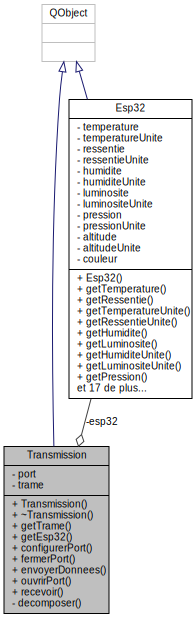
\includegraphics[height=550pt]{class_transmission__coll__graph}
\end{center}
\end{figure}
\subsubsection*{Connecteurs publics}
\begin{DoxyCompactItemize}
\item 
void \hyperlink{class_transmission_aa54a695d9d1c728ccab04f1d8030da41}{recevoir} ()
\begin{DoxyCompactList}\small\item\em Récupérer la trame émise. \end{DoxyCompactList}\item 
void \hyperlink{class_transmission_aeeccf41fd32a4bb17d3312d785aec98a}{ajouter\+Appareil} (const Q\+Bluetooth\+Device\+Info \&info)
\begin{DoxyCompactList}\small\item\em ajout les appareil trouver dans une list pour les afficher dans l\textquotesingle{}I\+HM \end{DoxyCompactList}\item 
void \hyperlink{class_transmission_a6945e6b653c6d46d7e13484811647e6e}{scan\+Terminer} ()
\begin{DoxyCompactList}\small\item\em fonction appeler quand le scan est fini \end{DoxyCompactList}\item 
void \hyperlink{class_transmission_ad231163c435936cc69149dd03aaaf473}{socket\+Connected} ()
\begin{DoxyCompactList}\small\item\em fonction appelée quand l\textquotesingle{}appareil est connecté \end{DoxyCompactList}\item 
void \hyperlink{class_transmission_a5b02dec98a34f14b341adf40cf520bdf}{socket\+Disconnected} ()
\begin{DoxyCompactList}\small\item\em fonction appelée quand l\textquotesingle{}appareil est deconnecté \end{DoxyCompactList}\item 
void \hyperlink{class_transmission_a3beab187cc2056a8f34bc6643fdc0e26}{socket\+Ready\+Read} ()
\begin{DoxyCompactList}\small\item\em methode appeler quand une trame est disponible \end{DoxyCompactList}\end{DoxyCompactItemize}
\subsubsection*{Signaux}
\begin{DoxyCompactItemize}
\item 
void \hyperlink{class_transmission_a489a1ee2f15aec3594b44f0a6152cbe6}{trame\+Esp32\+Recue} ()
\item 
void \hyperlink{class_transmission_a4501908a4480b9b2ea4358dc85dc438d}{trame\+Gps\+Recue} ()
\item 
void \hyperlink{class_transmission_af4627b741806b2d4eb05fae07f2b0588}{port\+Ouvert} ()
\item 
void \hyperlink{class_transmission_a4ec325c36d76fbf830253ff16e9783a7}{port\+Ferme} ()
\item 
void \hyperlink{class_transmission_a8789222ce8dc94d657d66a6edbbcc588}{nouvelle\+Appareil\+Disponible} ()
\item 
void \hyperlink{class_transmission_a2558a386d6888478f7d56c672a4855b3}{scanfini} ()
\item 
void \hyperlink{class_transmission_a76ba0e916b9e30615d563b78e26acbc2}{connecter} ()
\item 
void \hyperlink{class_transmission_aa3cfe0fc92fcc2147d239553820c983c}{deconnecter} ()
\item 
void \hyperlink{class_transmission_ad42d923341b19d450d27c7659ea51a58}{socket\+Erreur} ()
\end{DoxyCompactItemize}
\subsubsection*{Fonctions membres publiques}
\begin{DoxyCompactItemize}
\item 
\hyperlink{class_transmission_a1d8087d2d09b9ddd4fd6e8261daed9f3}{Transmission} (\hyperlink{class_q_object}{Q\+Object} $\ast$parent=nullptr)
\begin{DoxyCompactList}\small\item\em constructeur de la classe \hyperlink{class_transmission}{Transmission} \end{DoxyCompactList}\item 
\hyperlink{class_transmission_adcdc6012d99ddb1d0c3159d50984e146}{$\sim$\+Transmission} ()
\begin{DoxyCompactList}\small\item\em destructeur de la classe \hyperlink{class_transmission}{Transmission} \end{DoxyCompactList}\item 
Q\+String \hyperlink{class_transmission_a3fc179158c8c9e2cceba36423ef92505}{get\+Trame} () const 
\begin{DoxyCompactList}\small\item\em return la trame stockée \end{DoxyCompactList}\item 
\hyperlink{class_esp32}{Esp32} $\ast$ \hyperlink{class_transmission_afccd88f8be8c204a0960bc2d6970931f}{get\+Esp32} () const 
\begin{DoxyCompactList}\small\item\em return l\textquotesingle{}objet \hyperlink{class_esp32}{Esp32} \end{DoxyCompactList}\item 
\hyperlink{class_gps}{Gps} $\ast$ \hyperlink{class_transmission_aa5004c178152de5b94ef14e11e80792c}{get\+Gps} () const 
\begin{DoxyCompactList}\small\item\em return l\textquotesingle{}objet gps \end{DoxyCompactList}\item 
Q\+String\+List \hyperlink{class_transmission_a2a38d0633b4a27dfa3754efcd3db4f9c}{get\+Appareil\+Disponible} () const 
\begin{DoxyCompactList}\small\item\em return une liste des appareil bluetooth disponible \end{DoxyCompactList}\item 
Q\+String \hyperlink{class_transmission_adf65c6a49fbbc9d25b7b2fca2c410f99}{get\+Statut\+Bluetooth} () const 
\begin{DoxyCompactList}\small\item\em return la statut de la connexion avec l\textquotesingle{}appareil bluetooth \end{DoxyCompactList}\item 
void \hyperlink{class_transmission_a0680d6aab9c17d11e90566c359187ebc}{set\+Statut\+Bluetooth} (Q\+String \hyperlink{class_transmission_a01afc46fac8c712083225d5dd2386217}{statut\+Bluetooth})
\begin{DoxyCompactList}\small\item\em permet de modifier le statut de la connexion avec l\textquotesingle{}appareil bluetooth \end{DoxyCompactList}\item 
void \hyperlink{class_transmission_ad2c1d8838a1f7ed8d3599dba0a118a86}{set\+Appareil\+Disponible} (Q\+String \hyperlink{class_transmission_ada55d73f163440c8250102cfe74c05a1}{appareil\+Disponible})
\begin{DoxyCompactList}\small\item\em ajoute un appareil a la liste des appareil\+Disponible \end{DoxyCompactList}\item 
void \hyperlink{class_transmission_ab4e82ab30c181a8e0d0c0257ea0e1f56}{configurer\+Port} (Q\+String port\+Communication, Q\+String Debit\+Baud, Q\+String Bits\+Donnees, Q\+String Bits\+Stop)
\begin{DoxyCompactList}\small\item\em configure le port serie \end{DoxyCompactList}\item 
void \hyperlink{class_transmission_a14d36ad615852d6b630fbddf5787f3a3}{fermer\+Port} ()
\begin{DoxyCompactList}\small\item\em cette methode ferme le port serie \end{DoxyCompactList}\item 
void \hyperlink{class_transmission_a21e35372ada18cd35411c0e8c0984fd7}{envoyer\+Donnees} (Q\+String envoyer\+Trame)
\begin{DoxyCompactList}\small\item\em envoyer les données par le port serie ou bluetooth suivant le mode choisie \end{DoxyCompactList}\item 
void \hyperlink{class_transmission_a41d15e65be472e058b28869f8dfad392}{ouvrir\+Port} ()
\item 
void \hyperlink{class_transmission_a217b97344fdad09dbe226c55a8ac56b0}{demarrer\+Scan} ()
\begin{DoxyCompactList}\small\item\em cette fonction scan les appareils disponible \end{DoxyCompactList}\item 
void \hyperlink{class_transmission_a5a21d201dd0096f96aec12264c2f03d9}{connecter\+Appareil\+Bluetooth} (Q\+String appareil)
\begin{DoxyCompactList}\small\item\em Permets de se connecter à un appareil. \end{DoxyCompactList}\item 
void \hyperlink{class_transmission_afc5d716d53ee7039c3abf05f799327ae}{deconnecter\+Appareil\+Bluetooth} ()
\begin{DoxyCompactList}\small\item\em methode qui deconnecte l\textquotesingle{}appareil bluetooth connecter \end{DoxyCompactList}\end{DoxyCompactItemize}
\subsubsection*{Fonctions membres privées}
\begin{DoxyCompactItemize}
\item 
void \hyperlink{class_transmission_aa2977705ec793b10bf3212a13e67b097}{decomposer} ()
\begin{DoxyCompactList}\small\item\em Décompose la trame reçue. \end{DoxyCompactList}\item 
void \hyperlink{class_transmission_acc25e99cce910d23efe684cad233d30e}{decomposer\+Donnee\+Gps} ()
\begin{DoxyCompactList}\small\item\em Décompose la trame gps pour avoir la latitude et la longitude. \end{DoxyCompactList}\end{DoxyCompactItemize}
\subsubsection*{Attributs privés}
\begin{DoxyCompactItemize}
\item 
Q\+String \hyperlink{class_transmission_af2e63afdc212381aa023a3bcb48148c1}{trame}
\item 
Q\+String \hyperlink{class_transmission_a82596aa40988da67b05174375d9cfadb}{donnee\+Lat\+Dms}
\item 
Q\+String \hyperlink{class_transmission_abd43fbd8ce97a99ebfd1048a9b2297cf}{donnee\+Long\+Dms}
\item 
double \hyperlink{class_transmission_a4c7537ba62aa4ffa286ef269974e9571}{donne\+Lat\+DD}
\item 
double \hyperlink{class_transmission_a285721af01428c688b33c7af80f424f5}{donne\+Long\+DD}
\item 
Q\+String \hyperlink{class_transmission_aecd312863e33ce32d811895bc143b265}{signe\+Lat}
\item 
Q\+String \hyperlink{class_transmission_a80f29bafb41f10f5be97ebaced6e684a}{signe\+Long}
\item 
\hyperlink{class_esp32}{Esp32} $\ast$ \hyperlink{class_transmission_a06ec58d6f8fa4adff82f5b2ab911c461}{esp32}
\begin{DoxyCompactList}\small\item\em objet esp32 \end{DoxyCompactList}\item 
\hyperlink{class_gps}{Gps} $\ast$ \hyperlink{class_transmission_aebadfef439f114cb09e57ddb2e3188dc}{gps}
\begin{DoxyCompactList}\small\item\em objet gps \end{DoxyCompactList}\item 
Q\+Serial\+Port $\ast$ \hyperlink{class_transmission_a0ec8a06c44492c9b4f395e7c3b1e57b9}{port}
\begin{DoxyCompactList}\small\item\em objet port \end{DoxyCompactList}\item 
Q\+Bluetooth\+Device\+Discovery\+Agent $\ast$ \hyperlink{class_transmission_a70e442ca9125041564f79c40230ecd08}{scan}
\begin{DoxyCompactList}\small\item\em objet scan \end{DoxyCompactList}\item 
Q\+Low\+Energy\+Controller $\ast$ \hyperlink{class_transmission_a9b056d8291609ec049b91d0aed8e408a}{m\+\_\+controller}
\begin{DoxyCompactList}\small\item\em objet m\+\_\+controller \end{DoxyCompactList}\item 
Q\+Bluetooth\+Socket $\ast$ \hyperlink{class_transmission_a0b579c9da71d4b19f0504241ffbfae21}{socket}
\begin{DoxyCompactList}\small\item\em objet socket \end{DoxyCompactList}\item 
Q\+String \hyperlink{class_transmission_a01afc46fac8c712083225d5dd2386217}{statut\+Bluetooth}
\item 
Q\+String\+List \hyperlink{class_transmission_ada55d73f163440c8250102cfe74c05a1}{appareil\+Disponible}
\end{DoxyCompactItemize}


\subsubsection{Documentation des constructeurs et destructeur}
\index{Transmission@{Transmission}!Transmission@{Transmission}}
\index{Transmission@{Transmission}!Transmission@{Transmission}}
\paragraph[{\texorpdfstring{Transmission(\+Q\+Object $\ast$parent=nullptr)}{Transmission(QObject *parent=nullptr)}}]{\setlength{\rightskip}{0pt plus 5cm}Transmission\+::\+Transmission (
\begin{DoxyParamCaption}
\item[{{\bf Q\+Object} $\ast$}]{parent = {\ttfamily nullptr}}
\end{DoxyParamCaption}
)\hspace{0.3cm}{\ttfamily [explicit]}}\hypertarget{class_transmission_a1d8087d2d09b9ddd4fd6e8261daed9f3}{}\label{class_transmission_a1d8087d2d09b9ddd4fd6e8261daed9f3}

\begin{DoxyParams}{Paramètres}
{\em parent} & \\
\hline
\end{DoxyParams}


Références \hyperlink{class_transmission_aeeccf41fd32a4bb17d3312d785aec98a}{ajouter\+Appareil()}, \hyperlink{class_transmission_a217b97344fdad09dbe226c55a8ac56b0}{demarrer\+Scan()}, \hyperlink{class_transmission_a06ec58d6f8fa4adff82f5b2ab911c461}{esp32}, \hyperlink{class_transmission_aebadfef439f114cb09e57ddb2e3188dc}{gps}, \hyperlink{class_transmission_a0ec8a06c44492c9b4f395e7c3b1e57b9}{port}, \hyperlink{class_transmission_a70e442ca9125041564f79c40230ecd08}{scan}, \hyperlink{class_transmission_a6945e6b653c6d46d7e13484811647e6e}{scan\+Terminer()}, et \hyperlink{class_transmission_a0b579c9da71d4b19f0504241ffbfae21}{socket}.


\begin{DoxyCode}
00021                                           : \hyperlink{class_q_object}{QObject}(parent), \hyperlink{class_transmission_af2e63afdc212381aa023a3bcb48148c1}{trame}(\textcolor{stringliteral}{""}), 
      \hyperlink{class_transmission_a82596aa40988da67b05174375d9cfadb}{donneeLatDms}(\textcolor{stringliteral}{""}), \hyperlink{class_transmission_abd43fbd8ce97a99ebfd1048a9b2297cf}{donneeLongDms}(\textcolor{stringliteral}{""}), \hyperlink{class_transmission_a4c7537ba62aa4ffa286ef269974e9571}{donneLatDD}(0.), 
      \hyperlink{class_transmission_a285721af01428c688b33c7af80f424f5}{donneLongDD}(0.),\hyperlink{class_transmission_aecd312863e33ce32d811895bc143b265}{\(\backslash\)}
00022 \hyperlink{class_transmission_aecd312863e33ce32d811895bc143b265}{  signeLat}(\textcolor{stringliteral}{""}), \hyperlink{class_transmission_a80f29bafb41f10f5be97ebaced6e684a}{signeLong}(\textcolor{stringliteral}{""})
00023 \{
00024     \hyperlink{class_transmission_a06ec58d6f8fa4adff82f5b2ab911c461}{esp32} = \textcolor{keyword}{new} \hyperlink{class_esp32}{Esp32}(\textcolor{keyword}{this});
00025     \hyperlink{class_transmission_aebadfef439f114cb09e57ddb2e3188dc}{gps} = \textcolor{keyword}{new} \hyperlink{class_gps}{Gps}();
00026     \hyperlink{class_transmission_a0ec8a06c44492c9b4f395e7c3b1e57b9}{port} = \textcolor{keyword}{new} QSerialPort(\textcolor{keyword}{this});
00027     \hyperlink{class_transmission_a70e442ca9125041564f79c40230ecd08}{scan} = \textcolor{keyword}{new} QBluetoothDeviceDiscoveryAgent(\textcolor{keyword}{this});
00028     \hyperlink{class_transmission_a0b579c9da71d4b19f0504241ffbfae21}{socket} = \textcolor{keyword}{new} QBluetoothSocket(QBluetoothServiceInfo::RfcommProtocol);
00029 
00030     connect(\hyperlink{class_transmission_a70e442ca9125041564f79c40230ecd08}{scan}, SIGNAL(deviceDiscovered(QBluetoothDeviceInfo)), \textcolor{keyword}{this}, SLOT(
      \hyperlink{class_transmission_aeeccf41fd32a4bb17d3312d785aec98a}{ajouterAppareil}(QBluetoothDeviceInfo)));
00031     connect(\hyperlink{class_transmission_a70e442ca9125041564f79c40230ecd08}{scan}, SIGNAL(finished()), \textcolor{keyword}{this}, SLOT(\hyperlink{class_transmission_a6945e6b653c6d46d7e13484811647e6e}{scanTerminer}()));
00032 
00033     \hyperlink{class_transmission_a217b97344fdad09dbe226c55a8ac56b0}{demarrerScan}();
00034 \}
\end{DoxyCode}
\index{Transmission@{Transmission}!````~Transmission@{$\sim$\+Transmission}}
\index{````~Transmission@{$\sim$\+Transmission}!Transmission@{Transmission}}
\paragraph[{\texorpdfstring{$\sim$\+Transmission()}{~Transmission()}}]{\setlength{\rightskip}{0pt plus 5cm}Transmission\+::$\sim$\+Transmission (
\begin{DoxyParamCaption}
{}
\end{DoxyParamCaption}
)}\hypertarget{class_transmission_adcdc6012d99ddb1d0c3159d50984e146}{}\label{class_transmission_adcdc6012d99ddb1d0c3159d50984e146}
constructeur de la classe \hyperlink{class_transmission}{Transmission} 

Références \hyperlink{class_transmission_afc5d716d53ee7039c3abf05f799327ae}{deconnecter\+Appareil\+Bluetooth()}, \hyperlink{class_transmission_a14d36ad615852d6b630fbddf5787f3a3}{fermer\+Port()}, et \hyperlink{class_transmission_aebadfef439f114cb09e57ddb2e3188dc}{gps}.


\begin{DoxyCode}
00042 \{
00043     this->\hyperlink{class_transmission_a14d36ad615852d6b630fbddf5787f3a3}{fermerPort}();
00044     \textcolor{keyword}{delete} \hyperlink{class_transmission_aebadfef439f114cb09e57ddb2e3188dc}{gps};
00045     \hyperlink{class_transmission_afc5d716d53ee7039c3abf05f799327ae}{deconnecterAppareilBluetooth}();
00046 \}
\end{DoxyCode}


\subsubsection{Documentation des fonctions membres}
\index{Transmission@{Transmission}!ajouter\+Appareil@{ajouter\+Appareil}}
\index{ajouter\+Appareil@{ajouter\+Appareil}!Transmission@{Transmission}}
\paragraph[{\texorpdfstring{ajouter\+Appareil}{ajouterAppareil}}]{\setlength{\rightskip}{0pt plus 5cm}void Transmission\+::ajouter\+Appareil (
\begin{DoxyParamCaption}
\item[{const Q\+Bluetooth\+Device\+Info \&}]{info}
\end{DoxyParamCaption}
)\hspace{0.3cm}{\ttfamily [slot]}}\hypertarget{class_transmission_aeeccf41fd32a4bb17d3312d785aec98a}{}\label{class_transmission_aeeccf41fd32a4bb17d3312d785aec98a}
methode appeler quand une nouvelle trame et disponible


\begin{DoxyParams}{Paramètres}
{\em info} & \\
\hline
\end{DoxyParams}


Références \hyperlink{class_transmission_ada55d73f163440c8250102cfe74c05a1}{appareil\+Disponible}, et \hyperlink{class_transmission_ad2c1d8838a1f7ed8d3599dba0a118a86}{set\+Appareil\+Disponible()}.



Référencé par \hyperlink{class_transmission_a1d8087d2d09b9ddd4fd6e8261daed9f3}{Transmission()}.


\begin{DoxyCode}
00328 \{
00329     \textcolor{comment}{//QString appareilDisponible = QString("%1 %2").arg(info.address().toString()).arg(info.name());}
00330     QString \hyperlink{class_transmission_ada55d73f163440c8250102cfe74c05a1}{appareilDisponible} = info.address().toString();
00331 
00332     qDebug() << \textcolor{stringliteral}{"Appareil Bluetooth trouvé :"} << QString(\textcolor{stringliteral}{"%1 %2"}).arg(info.address().toString()).arg(info.
      name()) << endl;
00333 
00334     \hyperlink{class_transmission_ad2c1d8838a1f7ed8d3599dba0a118a86}{setAppareilDisponible}(appareilDisponible);
00335 \}
\end{DoxyCode}
\index{Transmission@{Transmission}!configurer\+Port@{configurer\+Port}}
\index{configurer\+Port@{configurer\+Port}!Transmission@{Transmission}}
\paragraph[{\texorpdfstring{configurer\+Port(\+Q\+String port\+Communication, Q\+String Debit\+Baud, Q\+String Bits\+Donnees, Q\+String Bits\+Stop)}{configurerPort(QString portCommunication, QString DebitBaud, QString BitsDonnees, QString BitsStop)}}]{\setlength{\rightskip}{0pt plus 5cm}void Transmission\+::configurer\+Port (
\begin{DoxyParamCaption}
\item[{Q\+String}]{port\+Communication, }
\item[{Q\+String}]{Debit\+Baud, }
\item[{Q\+String}]{Bits\+Donnees, }
\item[{Q\+String}]{Bits\+Stop}
\end{DoxyParamCaption}
)}\hypertarget{class_transmission_ab4e82ab30c181a8e0d0c0257ea0e1f56}{}\label{class_transmission_ab4e82ab30c181a8e0d0c0257ea0e1f56}
configurer le port de communication

modifier la liste des appareil bluetooth disponible 

Références \hyperlink{class_transmission_a41d15e65be472e058b28869f8dfad392}{ouvrir\+Port()}, et \hyperlink{class_transmission_a0ec8a06c44492c9b4f395e7c3b1e57b9}{port}.



Référencé par \hyperlink{class_ihm_a9ce167b94baead6e318bbd0c5254f842}{Ihm\+::on\+\_\+push\+Button\+Ouvrir\+Port\+\_\+clicked()}.


\begin{DoxyCode}
00152 \{
00153     \hyperlink{class_transmission_a0ec8a06c44492c9b4f395e7c3b1e57b9}{port} = \textcolor{keyword}{new} QSerialPort(portCommunication);
00154 
00155     \hyperlink{class_transmission_a0ec8a06c44492c9b4f395e7c3b1e57b9}{port}->setBaudRate(DebitBaud.toInt());
00156     \hyperlink{class_transmission_a0ec8a06c44492c9b4f395e7c3b1e57b9}{port}->setDataBits(QSerialPort::DataBits(BitsDonnees.toInt()));
00157     \hyperlink{class_transmission_a0ec8a06c44492c9b4f395e7c3b1e57b9}{port}->setParity(QSerialPort::NoParity);
00158     \hyperlink{class_transmission_a0ec8a06c44492c9b4f395e7c3b1e57b9}{port}->setStopBits(QSerialPort::StopBits(BitsStop.toInt()));
00159     \hyperlink{class_transmission_a0ec8a06c44492c9b4f395e7c3b1e57b9}{port}->setFlowControl(QSerialPort::NoFlowControl);
00160 
00161     \hyperlink{class_transmission_a41d15e65be472e058b28869f8dfad392}{ouvrirPort}();
00162 \}
\end{DoxyCode}
\index{Transmission@{Transmission}!connecter@{connecter}}
\index{connecter@{connecter}!Transmission@{Transmission}}
\paragraph[{\texorpdfstring{connecter}{connecter}}]{\setlength{\rightskip}{0pt plus 5cm}void Transmission\+::connecter (
\begin{DoxyParamCaption}
{}
\end{DoxyParamCaption}
)\hspace{0.3cm}{\ttfamily [signal]}}\hypertarget{class_transmission_a76ba0e916b9e30615d563b78e26acbc2}{}\label{class_transmission_a76ba0e916b9e30615d563b78e26acbc2}
signal emit quand le scan est terminé 

Référencé par \hyperlink{class_transmission_ad231163c435936cc69149dd03aaaf473}{socket\+Connected()}.

\index{Transmission@{Transmission}!connecter\+Appareil\+Bluetooth@{connecter\+Appareil\+Bluetooth}}
\index{connecter\+Appareil\+Bluetooth@{connecter\+Appareil\+Bluetooth}!Transmission@{Transmission}}
\paragraph[{\texorpdfstring{connecter\+Appareil\+Bluetooth(\+Q\+String appareil)}{connecterAppareilBluetooth(QString appareil)}}]{\setlength{\rightskip}{0pt plus 5cm}void Transmission\+::connecter\+Appareil\+Bluetooth (
\begin{DoxyParamCaption}
\item[{Q\+String}]{appareil}
\end{DoxyParamCaption}
)}\hypertarget{class_transmission_a5a21d201dd0096f96aec12264c2f03d9}{}\label{class_transmission_a5a21d201dd0096f96aec12264c2f03d9}
methode appelée pour demarrer le scan


\begin{DoxyParams}{Paramètres}
{\em appareil} & \\
\hline
\end{DoxyParams}


Références \hyperlink{class_transmission_a0680d6aab9c17d11e90566c359187ebc}{set\+Statut\+Bluetooth()}, \hyperlink{class_transmission_a0b579c9da71d4b19f0504241ffbfae21}{socket}, \hyperlink{class_transmission_ad231163c435936cc69149dd03aaaf473}{socket\+Connected()}, \hyperlink{class_transmission_a5b02dec98a34f14b341adf40cf520bdf}{socket\+Disconnected()}, \hyperlink{class_transmission_ad42d923341b19d450d27c7659ea51a58}{socket\+Erreur()}, et \hyperlink{class_transmission_a3beab187cc2056a8f34bc6643fdc0e26}{socket\+Ready\+Read()}.



Référencé par \hyperlink{class_ihm_abf61dda1820e5632485de93983c40196}{Ihm\+::on\+\_\+push\+Button\+Connexion\+\_\+clicked()}.


\begin{DoxyCode}
00356 \{
00357     connect(\hyperlink{class_transmission_a0b579c9da71d4b19f0504241ffbfae21}{socket}, SIGNAL(connected()), \textcolor{keyword}{this}, SLOT(\hyperlink{class_transmission_ad231163c435936cc69149dd03aaaf473}{socketConnected}()));
00358     connect(\hyperlink{class_transmission_a0b579c9da71d4b19f0504241ffbfae21}{socket}, SIGNAL(disconnected()), \textcolor{keyword}{this}, SLOT(\hyperlink{class_transmission_a5b02dec98a34f14b341adf40cf520bdf}{socketDisconnected}()));
00359     connect(\hyperlink{class_transmission_a0b579c9da71d4b19f0504241ffbfae21}{socket}, SIGNAL(readyRead()), \textcolor{keyword}{this}, SLOT(\hyperlink{class_transmission_a3beab187cc2056a8f34bc6643fdc0e26}{socketReadyRead}()));
00360     connect(\hyperlink{class_transmission_a0b579c9da71d4b19f0504241ffbfae21}{socket}, QOverload<QBluetoothSocket::SocketError>::of(&QBluetoothSocket::error),
00361         [=](QBluetoothSocket::SocketError error)
00362     \{
00363         qDebug() <<\_\_FUNCTION\_\_ << error;
00364         \hyperlink{class_transmission_a0680d6aab9c17d11e90566c359187ebc}{setStatutBluetooth}(\textcolor{stringliteral}{"Erreur"});
00365         emit \hyperlink{class_transmission_ad42d923341b19d450d27c7659ea51a58}{socketErreur}();
00366     \});
00367 
00368     QBluetoothAddress adresse = QBluetoothAddress(appareil);
00369     QBluetoothUuid uuid = QBluetoothUuid(QBluetoothUuid::SerialPort);
00370     \hyperlink{class_transmission_a0b579c9da71d4b19f0504241ffbfae21}{socket}->connectToService(adresse, uuid);
00371     \hyperlink{class_transmission_a0b579c9da71d4b19f0504241ffbfae21}{socket}->open(QIODevice::ReadWrite);
00372 \}
\end{DoxyCode}
\index{Transmission@{Transmission}!decomposer@{decomposer}}
\index{decomposer@{decomposer}!Transmission@{Transmission}}
\paragraph[{\texorpdfstring{decomposer()}{decomposer()}}]{\setlength{\rightskip}{0pt plus 5cm}void Transmission\+::decomposer (
\begin{DoxyParamCaption}
{}
\end{DoxyParamCaption}
)\hspace{0.3cm}{\ttfamily [private]}}\hypertarget{class_transmission_aa2977705ec793b10bf3212a13e67b097}{}\label{class_transmission_aa2977705ec793b10bf3212a13e67b097}
stockage du statut de la connexion bluetooth 

Références \hyperlink{class_transmission_a06ec58d6f8fa4adff82f5b2ab911c461}{esp32}, \hyperlink{class_esp32_aeb2268155501f27e36e6a7c6caa15412}{Esp32\+::set\+Altitude()}, \hyperlink{class_esp32_a69b0c6a1c0a31e043b715be3fc40ded1}{Esp32\+::set\+Altitude\+Unite()}, \hyperlink{class_esp32_a32d0d1abb41a3762a54e9f5a33b3b247}{Esp32\+::set\+Couleur\+Led()}, \hyperlink{class_esp32_a029c94bf405887eb890b3381ac176a9a}{Esp32\+::set\+Humidite()}, \hyperlink{class_esp32_ae9b2704f36bcd246668354d0ac06ea35}{Esp32\+::set\+Humidite\+Unite()}, \hyperlink{class_esp32_ae60b48e8c808a5108402d5b9f03590ac}{Esp32\+::set\+Luminosite()}, \hyperlink{class_esp32_a36450bcd23e7676d1f0a46e8bec31275}{Esp32\+::set\+Luminosite\+Unite()}, \hyperlink{class_esp32_a583358abbf0b279dabb5a2976f1783de}{Esp32\+::set\+Pression()}, \hyperlink{class_esp32_a3c6dd57f955aef0738c48be705538337}{Esp32\+::set\+Pression\+Unite()}, \hyperlink{class_esp32_a85dc760b771c9233fa094a49679d9286}{Esp32\+::set\+Ressentie()}, \hyperlink{class_esp32_abf8a7f9942150b6c17cc5d1cc7b0fc8a}{Esp32\+::set\+Ressentie\+Unite()}, \hyperlink{class_esp32_a8e7a509ed5704bee4bc527ae297f14f0}{Esp32\+::set\+Temperature()}, \hyperlink{class_esp32_a709c261e1cea7b6bbd2ea1b09b1d7ec0}{Esp32\+::set\+Temperature\+Unite()}, \hyperlink{class_transmission_af2e63afdc212381aa023a3bcb48148c1}{trame}, et \hyperlink{class_transmission_a489a1ee2f15aec3594b44f0a6152cbe6}{trame\+Esp32\+Recue()}.



Référencé par \hyperlink{class_transmission_aa54a695d9d1c728ccab04f1d8030da41}{recevoir()}, et \hyperlink{class_transmission_a3beab187cc2056a8f34bc6643fdc0e26}{socket\+Ready\+Read()}.


\begin{DoxyCode}
00187 \{
00188     \textcolor{keywordflow}{if}(\hyperlink{class_transmission_af2e63afdc212381aa023a3bcb48148c1}{trame}.startsWith(\textcolor{stringliteral}{"SONDE"}) && \hyperlink{class_transmission_af2e63afdc212381aa023a3bcb48148c1}{trame}.endsWith(\textcolor{stringliteral}{"\(\backslash\)r\(\backslash\)n"}))
00189     \{
00190         \hyperlink{class_transmission_a06ec58d6f8fa4adff82f5b2ab911c461}{esp32}->\hyperlink{class_esp32_a8e7a509ed5704bee4bc527ae297f14f0}{setTemperature}(\hyperlink{class_transmission_af2e63afdc212381aa023a3bcb48148c1}{trame}.section(\textcolor{stringliteral}{";"},1,1).toDouble());
00191         \hyperlink{class_transmission_a06ec58d6f8fa4adff82f5b2ab911c461}{esp32}->\hyperlink{class_esp32_a709c261e1cea7b6bbd2ea1b09b1d7ec0}{setTemperatureUnite}(\hyperlink{class_transmission_af2e63afdc212381aa023a3bcb48148c1}{trame}.section(\textcolor{stringliteral}{";"},2,2));
00192         \hyperlink{class_transmission_a06ec58d6f8fa4adff82f5b2ab911c461}{esp32}->\hyperlink{class_esp32_a85dc760b771c9233fa094a49679d9286}{setRessentie}(\hyperlink{class_transmission_af2e63afdc212381aa023a3bcb48148c1}{trame}.section(\textcolor{stringliteral}{";"},3,3).toDouble());
00193         \hyperlink{class_transmission_a06ec58d6f8fa4adff82f5b2ab911c461}{esp32}->\hyperlink{class_esp32_abf8a7f9942150b6c17cc5d1cc7b0fc8a}{setRessentieUnite}(\hyperlink{class_transmission_af2e63afdc212381aa023a3bcb48148c1}{trame}.section(\textcolor{stringliteral}{";"},4,4));
00194         \hyperlink{class_transmission_a06ec58d6f8fa4adff82f5b2ab911c461}{esp32}->\hyperlink{class_esp32_a029c94bf405887eb890b3381ac176a9a}{setHumidite}(\hyperlink{class_transmission_af2e63afdc212381aa023a3bcb48148c1}{trame}.section(\textcolor{stringliteral}{";"},5,5).toInt());
00195         \hyperlink{class_transmission_a06ec58d6f8fa4adff82f5b2ab911c461}{esp32}->\hyperlink{class_esp32_ae9b2704f36bcd246668354d0ac06ea35}{setHumiditeUnite}(\hyperlink{class_transmission_af2e63afdc212381aa023a3bcb48148c1}{trame}.section(\textcolor{stringliteral}{";"},6,6));
00196         \hyperlink{class_transmission_a06ec58d6f8fa4adff82f5b2ab911c461}{esp32}->\hyperlink{class_esp32_ae60b48e8c808a5108402d5b9f03590ac}{setLuminosite}(\hyperlink{class_transmission_af2e63afdc212381aa023a3bcb48148c1}{trame}.section(\textcolor{stringliteral}{";"},7,7).toInt());
00197         \hyperlink{class_transmission_a06ec58d6f8fa4adff82f5b2ab911c461}{esp32}->\hyperlink{class_esp32_a36450bcd23e7676d1f0a46e8bec31275}{setLuminositeUnite}(\hyperlink{class_transmission_af2e63afdc212381aa023a3bcb48148c1}{trame}.section(\textcolor{stringliteral}{";"},8,8));
00198         \hyperlink{class_transmission_a06ec58d6f8fa4adff82f5b2ab911c461}{esp32}->\hyperlink{class_esp32_a583358abbf0b279dabb5a2976f1783de}{setPression}(\hyperlink{class_transmission_af2e63afdc212381aa023a3bcb48148c1}{trame}.section(\textcolor{stringliteral}{";"},9,9).toInt());
00199         \hyperlink{class_transmission_a06ec58d6f8fa4adff82f5b2ab911c461}{esp32}->\hyperlink{class_esp32_a3c6dd57f955aef0738c48be705538337}{setPressionUnite}(\hyperlink{class_transmission_af2e63afdc212381aa023a3bcb48148c1}{trame}.section(\textcolor{stringliteral}{";"},10,10));
00200         \hyperlink{class_transmission_a06ec58d6f8fa4adff82f5b2ab911c461}{esp32}->\hyperlink{class_esp32_aeb2268155501f27e36e6a7c6caa15412}{setAltitude}(\hyperlink{class_transmission_af2e63afdc212381aa023a3bcb48148c1}{trame}.section(\textcolor{stringliteral}{";"},11,11).toInt());
00201         \hyperlink{class_transmission_a06ec58d6f8fa4adff82f5b2ab911c461}{esp32}->\hyperlink{class_esp32_a69b0c6a1c0a31e043b715be3fc40ded1}{setAltitudeUnite}(\hyperlink{class_transmission_af2e63afdc212381aa023a3bcb48148c1}{trame}.section(\textcolor{stringliteral}{";"},12,12));
00202         \hyperlink{class_transmission_a06ec58d6f8fa4adff82f5b2ab911c461}{esp32}->\hyperlink{class_esp32_a32d0d1abb41a3762a54e9f5a33b3b247}{setCouleurLed}(\hyperlink{class_transmission_af2e63afdc212381aa023a3bcb48148c1}{trame}.section(\textcolor{stringliteral}{";"},17,17).toInt());
00203     \}
00204     emit \hyperlink{class_transmission_a489a1ee2f15aec3594b44f0a6152cbe6}{trameEsp32Recue}();
00205 \}
\end{DoxyCode}
\index{Transmission@{Transmission}!decomposer\+Donnee\+Gps@{decomposer\+Donnee\+Gps}}
\index{decomposer\+Donnee\+Gps@{decomposer\+Donnee\+Gps}!Transmission@{Transmission}}
\paragraph[{\texorpdfstring{decomposer\+Donnee\+Gps()}{decomposerDonneeGps()}}]{\setlength{\rightskip}{0pt plus 5cm}void Transmission\+::decomposer\+Donnee\+Gps (
\begin{DoxyParamCaption}
{}
\end{DoxyParamCaption}
)\hspace{0.3cm}{\ttfamily [private]}}\hypertarget{class_transmission_acc25e99cce910d23efe684cad233d30e}{}\label{class_transmission_acc25e99cce910d23efe684cad233d30e}
decomposition de la trame recu 

Références \hyperlink{class_transmission_a82596aa40988da67b05174375d9cfadb}{donnee\+Lat\+Dms}, \hyperlink{class_transmission_abd43fbd8ce97a99ebfd1048a9b2297cf}{donnee\+Long\+Dms}, \hyperlink{class_transmission_a4c7537ba62aa4ffa286ef269974e9571}{donne\+Lat\+DD}, \hyperlink{class_transmission_a285721af01428c688b33c7af80f424f5}{donne\+Long\+DD}, \hyperlink{class_transmission_aebadfef439f114cb09e57ddb2e3188dc}{gps}, \hyperlink{class_gps_aaabf328f0bbcdbb9c2901e30b6edccc7}{Gps\+::set\+Latitude()}, \hyperlink{class_gps_a2d9ca07c62c5bae627c2131062a1236a}{Gps\+::set\+Longitude()}, \hyperlink{class_transmission_aecd312863e33ce32d811895bc143b265}{signe\+Lat}, \hyperlink{class_transmission_a80f29bafb41f10f5be97ebaced6e684a}{signe\+Long}, \hyperlink{class_transmission_af2e63afdc212381aa023a3bcb48148c1}{trame}, et \hyperlink{class_transmission_a4501908a4480b9b2ea4358dc85dc438d}{trame\+Gps\+Recue()}.



Référencé par \hyperlink{class_transmission_aa54a695d9d1c728ccab04f1d8030da41}{recevoir()}.


\begin{DoxyCode}
00213 \{
00214     \textcolor{keywordflow}{if}(\hyperlink{class_transmission_af2e63afdc212381aa023a3bcb48148c1}{trame}.startsWith(\textcolor{stringliteral}{"$GPGGA"}) && \hyperlink{class_transmission_af2e63afdc212381aa023a3bcb48148c1}{trame}.endsWith(\textcolor{stringliteral}{"\(\backslash\)r\(\backslash\)n"}))
00215     \{
00216         \hyperlink{class_transmission_a82596aa40988da67b05174375d9cfadb}{donneeLatDms} = \hyperlink{class_transmission_af2e63afdc212381aa023a3bcb48148c1}{trame}.section(\textcolor{stringliteral}{","},2,2);
00217         \hyperlink{class_transmission_abd43fbd8ce97a99ebfd1048a9b2297cf}{donneeLongDms} = \hyperlink{class_transmission_af2e63afdc212381aa023a3bcb48148c1}{trame}.section(\textcolor{stringliteral}{","},4,4);
00218         \hyperlink{class_transmission_aecd312863e33ce32d811895bc143b265}{signeLat} = \hyperlink{class_transmission_af2e63afdc212381aa023a3bcb48148c1}{trame}.section(\textcolor{stringliteral}{","},3,3);
00219         \hyperlink{class_transmission_a80f29bafb41f10f5be97ebaced6e684a}{signeLong} = \hyperlink{class_transmission_af2e63afdc212381aa023a3bcb48148c1}{trame}.section(\textcolor{stringliteral}{","},5,5);
00220 
00221         \textcolor{keywordflow}{if}(\hyperlink{class_transmission_aecd312863e33ce32d811895bc143b265}{signeLat} == \textcolor{stringliteral}{"N"})
00222         \{
00223             \hyperlink{class_transmission_a4c7537ba62aa4ffa286ef269974e9571}{donneLatDD} = \hyperlink{class_transmission_a82596aa40988da67b05174375d9cfadb}{donneeLatDms}.left(2).toDouble() + 
      \hyperlink{class_transmission_a82596aa40988da67b05174375d9cfadb}{donneeLatDms}.mid(2,2).toDouble()/60 + \hyperlink{class_transmission_a82596aa40988da67b05174375d9cfadb}{donneeLatDms}.mid(5,2).toDouble()/3600;
00224             qDebug() << \textcolor{stringliteral}{"latitude DD:"} << \hyperlink{class_transmission_a4c7537ba62aa4ffa286ef269974e9571}{donneLatDD} << endl;
00225             \hyperlink{class_transmission_aebadfef439f114cb09e57ddb2e3188dc}{gps}->\hyperlink{class_gps_aaabf328f0bbcdbb9c2901e30b6edccc7}{setLatitude}(\hyperlink{class_transmission_a4c7537ba62aa4ffa286ef269974e9571}{donneLatDD});
00226         \}
00227         \textcolor{keywordflow}{else} \textcolor{keywordflow}{if}(\hyperlink{class_transmission_a80f29bafb41f10f5be97ebaced6e684a}{signeLong} == \textcolor{stringliteral}{"S"})
00228         \{
00229             \hyperlink{class_transmission_a4c7537ba62aa4ffa286ef269974e9571}{donneLatDD} = \hyperlink{class_transmission_a82596aa40988da67b05174375d9cfadb}{donneeLatDms}.left(2).toDouble() + 
      \hyperlink{class_transmission_a82596aa40988da67b05174375d9cfadb}{donneeLatDms}.mid(2,2).toDouble()/60 + \hyperlink{class_transmission_a82596aa40988da67b05174375d9cfadb}{donneeLatDms}.mid(5,2).toDouble()/3600;
00230             qDebug() << \textcolor{stringliteral}{"latitude DD:"} << \hyperlink{class_transmission_a4c7537ba62aa4ffa286ef269974e9571}{donneLatDD} * -1 << endl;
00231             \hyperlink{class_transmission_aebadfef439f114cb09e57ddb2e3188dc}{gps}->\hyperlink{class_gps_aaabf328f0bbcdbb9c2901e30b6edccc7}{setLatitude}(\hyperlink{class_transmission_a4c7537ba62aa4ffa286ef269974e9571}{donneLatDD} * -1);
00232         \}
00233 
00234         \textcolor{keywordflow}{if}(\hyperlink{class_transmission_a80f29bafb41f10f5be97ebaced6e684a}{signeLong} == \textcolor{stringliteral}{"E"})
00235         \{
00236             \hyperlink{class_transmission_a285721af01428c688b33c7af80f424f5}{donneLongDD} = \hyperlink{class_transmission_abd43fbd8ce97a99ebfd1048a9b2297cf}{donneeLongDms}.left(3).toDouble() + 
      \hyperlink{class_transmission_abd43fbd8ce97a99ebfd1048a9b2297cf}{donneeLongDms}.mid(2,2).toDouble()/60 + \hyperlink{class_transmission_abd43fbd8ce97a99ebfd1048a9b2297cf}{donneeLongDms}.mid(5,2).toDouble()/3600;
00237             qDebug() << \textcolor{stringliteral}{"longitude DD:"} << \hyperlink{class_transmission_a285721af01428c688b33c7af80f424f5}{donneLongDD} << endl;
00238             \hyperlink{class_transmission_aebadfef439f114cb09e57ddb2e3188dc}{gps}->\hyperlink{class_gps_a2d9ca07c62c5bae627c2131062a1236a}{setLongitude}(\hyperlink{class_transmission_a285721af01428c688b33c7af80f424f5}{donneLongDD});
00239         \}
00240         \textcolor{keywordflow}{else} \textcolor{keywordflow}{if}(\hyperlink{class_transmission_aecd312863e33ce32d811895bc143b265}{signeLat} == \textcolor{stringliteral}{"W"})
00241         \{
00242             \hyperlink{class_transmission_a285721af01428c688b33c7af80f424f5}{donneLongDD} = \hyperlink{class_transmission_abd43fbd8ce97a99ebfd1048a9b2297cf}{donneeLongDms}.left(3).toDouble() + 
      \hyperlink{class_transmission_abd43fbd8ce97a99ebfd1048a9b2297cf}{donneeLongDms}.mid(2,2).toDouble()/60 + \hyperlink{class_transmission_abd43fbd8ce97a99ebfd1048a9b2297cf}{donneeLongDms}.mid(5,2).toDouble()/3600;
00243             qDebug() << \textcolor{stringliteral}{"longitude DD:"} << \hyperlink{class_transmission_a285721af01428c688b33c7af80f424f5}{donneLongDD} * -1 << endl;
00244             \hyperlink{class_transmission_aebadfef439f114cb09e57ddb2e3188dc}{gps}->\hyperlink{class_gps_a2d9ca07c62c5bae627c2131062a1236a}{setLongitude}(\hyperlink{class_transmission_a285721af01428c688b33c7af80f424f5}{donneLongDD} * -1);
00245         \}
00246     \}
00247     emit \hyperlink{class_transmission_a4501908a4480b9b2ea4358dc85dc438d}{trameGpsRecue}();
00248 \}
\end{DoxyCode}
\index{Transmission@{Transmission}!deconnecter@{deconnecter}}
\index{deconnecter@{deconnecter}!Transmission@{Transmission}}
\paragraph[{\texorpdfstring{deconnecter}{deconnecter}}]{\setlength{\rightskip}{0pt plus 5cm}void Transmission\+::deconnecter (
\begin{DoxyParamCaption}
{}
\end{DoxyParamCaption}
)\hspace{0.3cm}{\ttfamily [signal]}}\hypertarget{class_transmission_aa3cfe0fc92fcc2147d239553820c983c}{}\label{class_transmission_aa3cfe0fc92fcc2147d239553820c983c}
signal emit quand l\textquotesingle{}appareil est connecté 

Référencé par \hyperlink{class_transmission_a5b02dec98a34f14b341adf40cf520bdf}{socket\+Disconnected()}.

\index{Transmission@{Transmission}!deconnecter\+Appareil\+Bluetooth@{deconnecter\+Appareil\+Bluetooth}}
\index{deconnecter\+Appareil\+Bluetooth@{deconnecter\+Appareil\+Bluetooth}!Transmission@{Transmission}}
\paragraph[{\texorpdfstring{deconnecter\+Appareil\+Bluetooth()}{deconnecterAppareilBluetooth()}}]{\setlength{\rightskip}{0pt plus 5cm}void Transmission\+::deconnecter\+Appareil\+Bluetooth (
\begin{DoxyParamCaption}
{}
\end{DoxyParamCaption}
)}\hypertarget{class_transmission_afc5d716d53ee7039c3abf05f799327ae}{}\label{class_transmission_afc5d716d53ee7039c3abf05f799327ae}
methode appelée pour connecter un appareil bluetooth 

Références \hyperlink{class_transmission_a0b579c9da71d4b19f0504241ffbfae21}{socket}.



Référencé par \hyperlink{class_ihm_ad176c58fb3c583286544f010ac006b66}{Ihm\+::on\+\_\+push\+Button\+Deconnexion\+\_\+clicked()}, et \hyperlink{class_transmission_adcdc6012d99ddb1d0c3159d50984e146}{$\sim$\+Transmission()}.


\begin{DoxyCode}
00380 \{
00381     \textcolor{keywordflow}{if} (\hyperlink{class_transmission_a0b579c9da71d4b19f0504241ffbfae21}{socket}->isOpen())
00382         \{
00383             \hyperlink{class_transmission_a0b579c9da71d4b19f0504241ffbfae21}{socket}->close();
00384         \}
00385 \}
\end{DoxyCode}
\index{Transmission@{Transmission}!demarrer\+Scan@{demarrer\+Scan}}
\index{demarrer\+Scan@{demarrer\+Scan}!Transmission@{Transmission}}
\paragraph[{\texorpdfstring{demarrer\+Scan()}{demarrerScan()}}]{\setlength{\rightskip}{0pt plus 5cm}void Transmission\+::demarrer\+Scan (
\begin{DoxyParamCaption}
{}
\end{DoxyParamCaption}
)}\hypertarget{class_transmission_a217b97344fdad09dbe226c55a8ac56b0}{}\label{class_transmission_a217b97344fdad09dbe226c55a8ac56b0}
Méthode appelée pour ouvrir le port série 

Références \hyperlink{class_transmission_ada55d73f163440c8250102cfe74c05a1}{appareil\+Disponible}, et \hyperlink{class_transmission_a70e442ca9125041564f79c40230ecd08}{scan}.



Référencé par \hyperlink{class_ihm_a277763bdb63ed529aafba7db513cb630}{Ihm\+::on\+\_\+push\+Button\+Scan\+\_\+clicked()}, et \hyperlink{class_transmission_a1d8087d2d09b9ddd4fd6e8261daed9f3}{Transmission()}.


\begin{DoxyCode}
00315 \{
00316     qDebug() << \textcolor{stringliteral}{"scan en cour..."} << endl;
00317     \hyperlink{class_transmission_ada55d73f163440c8250102cfe74c05a1}{appareilDisponible}.clear();
00318     \hyperlink{class_transmission_a70e442ca9125041564f79c40230ecd08}{scan}->start();
00319 \}
\end{DoxyCode}
\index{Transmission@{Transmission}!envoyer\+Donnees@{envoyer\+Donnees}}
\index{envoyer\+Donnees@{envoyer\+Donnees}!Transmission@{Transmission}}
\paragraph[{\texorpdfstring{envoyer\+Donnees(\+Q\+String envoyer\+Trame)}{envoyerDonnees(QString envoyerTrame)}}]{\setlength{\rightskip}{0pt plus 5cm}void Transmission\+::envoyer\+Donnees (
\begin{DoxyParamCaption}
\item[{Q\+String}]{envoyer\+Trame}
\end{DoxyParamCaption}
)}\hypertarget{class_transmission_a21e35372ada18cd35411c0e8c0984fd7}{}\label{class_transmission_a21e35372ada18cd35411c0e8c0984fd7}
fermer le port de transmission


\begin{DoxyParams}{Paramètres}
{\em envoyer\+Trame} & \\
\hline
\end{DoxyParams}


Références \hyperlink{class_transmission_a0ec8a06c44492c9b4f395e7c3b1e57b9}{port}, \hyperlink{class_transmission_a4ec325c36d76fbf830253ff16e9783a7}{port\+Ferme()}, \hyperlink{class_transmission_a0b579c9da71d4b19f0504241ffbfae21}{socket}, et \hyperlink{class_transmission_af2e63afdc212381aa023a3bcb48148c1}{trame}.



Référencé par \hyperlink{class_ihm_afd32da9e614eba44bb1d3630b48e6075}{Ihm\+::on\+\_\+push\+Button\+Envoyer\+Trame\+\_\+clicked()}, \hyperlink{class_ihm_a1e328a2e8165bbef347e901f1bc5534d}{Ihm\+::on\+\_\+radio\+Button\+Led\+Off\+\_\+clicked()}, \hyperlink{class_ihm_a7e000e198b11fc38a4459f7749561ded}{Ihm\+::on\+\_\+radio\+Button\+Led\+Orange\+\_\+clicked()}, \hyperlink{class_ihm_a731ee780915cb90a5dfb11f2e02144c9}{Ihm\+::on\+\_\+radio\+Button\+Led\+Rouge\+\_\+clicked()}, et \hyperlink{class_ihm_afef5bfaa83383427e615d21d9474f466}{Ihm\+::on\+\_\+radio\+Button\+Led\+Vert\+\_\+clicked()}.


\begin{DoxyCode}
00286 \{
00287     \textcolor{keywordflow}{if}(\hyperlink{class_transmission_a0ec8a06c44492c9b4f395e7c3b1e57b9}{port}->isOpen())
00288     \{
00289         \textcolor{keyword}{const} \textcolor{keywordtype}{char}* \hyperlink{class_transmission_af2e63afdc212381aa023a3bcb48148c1}{trame} = envoyerTrame.toStdString().c\_str();
00290         \hyperlink{class_transmission_a0ec8a06c44492c9b4f395e7c3b1e57b9}{port}->write(trame);
00291 
00292         qDebug() << \_\_FUNCTION\_\_ << \textcolor{stringliteral}{": "} << trame << endl;
00293     \}
00294 
00295     \textcolor{keywordflow}{if}(\hyperlink{class_transmission_a0b579c9da71d4b19f0504241ffbfae21}{socket}->isOpen())
00296     \{
00297         \textcolor{keyword}{const} \textcolor{keywordtype}{char}* trame = envoyerTrame.toStdString().c\_str();
00298         \hyperlink{class_transmission_a0b579c9da71d4b19f0504241ffbfae21}{socket}->write(trame);
00299 
00300         qDebug() << \_\_FUNCTION\_\_ << \textcolor{stringliteral}{": "} << trame << endl;
00301     \}
00302 
00303     \textcolor{keywordflow}{if}(!\hyperlink{class_transmission_a0b579c9da71d4b19f0504241ffbfae21}{socket}->isOpen() && !\hyperlink{class_transmission_a0ec8a06c44492c9b4f395e7c3b1e57b9}{port}->isOpen())
00304     \{
00305         emit \hyperlink{class_transmission_a4ec325c36d76fbf830253ff16e9783a7}{portFerme}();
00306     \}
00307 \}
\end{DoxyCode}
\index{Transmission@{Transmission}!fermer\+Port@{fermer\+Port}}
\index{fermer\+Port@{fermer\+Port}!Transmission@{Transmission}}
\paragraph[{\texorpdfstring{fermer\+Port()}{fermerPort()}}]{\setlength{\rightskip}{0pt plus 5cm}void Transmission\+::fermer\+Port (
\begin{DoxyParamCaption}
{}
\end{DoxyParamCaption}
)}\hypertarget{class_transmission_a14d36ad615852d6b630fbddf5787f3a3}{}\label{class_transmission_a14d36ad615852d6b630fbddf5787f3a3}
configurer le port de transmission 

Références \hyperlink{class_transmission_a0ec8a06c44492c9b4f395e7c3b1e57b9}{port}, et \hyperlink{class_transmission_a4ec325c36d76fbf830253ff16e9783a7}{port\+Ferme()}.



Référencé par \hyperlink{class_ihm_abcdae03ce7e83266fb9d3e795df8a171}{Ihm\+::on\+\_\+push\+Button\+Fermer\+Port\+\_\+clicked()}, et \hyperlink{class_transmission_adcdc6012d99ddb1d0c3159d50984e146}{$\sim$\+Transmission()}.


\begin{DoxyCode}
00170 \{
00171     \textcolor{keywordflow}{if}(\hyperlink{class_transmission_a0ec8a06c44492c9b4f395e7c3b1e57b9}{port}->isOpen())
00172     \{
00173         \hyperlink{class_transmission_a0ec8a06c44492c9b4f395e7c3b1e57b9}{port}->close();
00174 
00175         qDebug() << \_\_FUNCTION\_\_ << \textcolor{stringliteral}{": "} <<\textcolor{stringliteral}{"port fermer"} <<endl;
00176 
00177         emit \hyperlink{class_transmission_a4ec325c36d76fbf830253ff16e9783a7}{portFerme}();
00178     \}
00179 \}
\end{DoxyCode}
\index{Transmission@{Transmission}!get\+Appareil\+Disponible@{get\+Appareil\+Disponible}}
\index{get\+Appareil\+Disponible@{get\+Appareil\+Disponible}!Transmission@{Transmission}}
\paragraph[{\texorpdfstring{get\+Appareil\+Disponible() const }{getAppareilDisponible() const }}]{\setlength{\rightskip}{0pt plus 5cm}Q\+String\+List Transmission\+::get\+Appareil\+Disponible (
\begin{DoxyParamCaption}
{}
\end{DoxyParamCaption}
) const}\hypertarget{class_transmission_a2a38d0633b4a27dfa3754efcd3db4f9c}{}\label{class_transmission_a2a38d0633b4a27dfa3754efcd3db4f9c}
recuperer l\textquotesingle{}objet gps

\begin{DoxyReturn}{Renvoie}
Q\+String\+List 
\end{DoxyReturn}


Références \hyperlink{class_transmission_ada55d73f163440c8250102cfe74c05a1}{appareil\+Disponible}.



Référencé par \hyperlink{class_ihm_a9d9ac22e5d73a010bc75a1fcf2e7ddcb}{Ihm\+::mettre\+Ajour\+Appareil\+Bluetooth\+Disponible()}.


\begin{DoxyCode}
00088 \{
00089     \textcolor{keywordflow}{return} \hyperlink{class_transmission_ada55d73f163440c8250102cfe74c05a1}{appareilDisponible};
00090 \}
\end{DoxyCode}
\index{Transmission@{Transmission}!get\+Esp32@{get\+Esp32}}
\index{get\+Esp32@{get\+Esp32}!Transmission@{Transmission}}
\paragraph[{\texorpdfstring{get\+Esp32() const }{getEsp32() const }}]{\setlength{\rightskip}{0pt plus 5cm}{\bf Esp32} $\ast$ Transmission\+::get\+Esp32 (
\begin{DoxyParamCaption}
{}
\end{DoxyParamCaption}
) const}\hypertarget{class_transmission_afccd88f8be8c204a0960bc2d6970931f}{}\label{class_transmission_afccd88f8be8c204a0960bc2d6970931f}
recuperer la trame

\begin{DoxyReturn}{Renvoie}
\hyperlink{class_esp32}{Esp32} 
\end{DoxyReturn}


Références \hyperlink{class_transmission_a06ec58d6f8fa4adff82f5b2ab911c461}{esp32}.



Référencé par \hyperlink{class_ihm_a7c0a160f30e11a4f8d56b174e07566fe}{Ihm\+::actualiser\+Donnee()}, et \hyperlink{class_ihm_af0426507c2130aefd01bdb4f825ae168}{Ihm\+::modifier\+Etat\+Led()}.


\begin{DoxyCode}
00066 \{
00067     \textcolor{keywordflow}{return} \hyperlink{class_transmission_a06ec58d6f8fa4adff82f5b2ab911c461}{esp32};
00068 \}
\end{DoxyCode}
\index{Transmission@{Transmission}!get\+Gps@{get\+Gps}}
\index{get\+Gps@{get\+Gps}!Transmission@{Transmission}}
\paragraph[{\texorpdfstring{get\+Gps() const }{getGps() const }}]{\setlength{\rightskip}{0pt plus 5cm}{\bf Gps} $\ast$ Transmission\+::get\+Gps (
\begin{DoxyParamCaption}
{}
\end{DoxyParamCaption}
) const}\hypertarget{class_transmission_aa5004c178152de5b94ef14e11e80792c}{}\label{class_transmission_aa5004c178152de5b94ef14e11e80792c}
recuperer l\textquotesingle{}objet esp32

\begin{DoxyReturn}{Renvoie}
\hyperlink{class_esp32}{Esp32} 
\end{DoxyReturn}


Références \hyperlink{class_transmission_aebadfef439f114cb09e57ddb2e3188dc}{gps}.



Référencé par \hyperlink{class_ihm_a3ca276093d65c42a5fc5a87cbca1972a}{Ihm\+::actualiser\+Donnee\+Gps()}, et \hyperlink{class_ihm_a850d1c97ed5fe5ba3cf3aa85d81872cd}{Ihm\+::on\+\_\+push\+Button\+Envoyer\+Coordonnee\+\_\+clicked()}.


\begin{DoxyCode}
00077 \{
00078     \textcolor{keywordflow}{return} \hyperlink{class_transmission_aebadfef439f114cb09e57ddb2e3188dc}{gps};
00079 \}
\end{DoxyCode}
\index{Transmission@{Transmission}!get\+Statut\+Bluetooth@{get\+Statut\+Bluetooth}}
\index{get\+Statut\+Bluetooth@{get\+Statut\+Bluetooth}!Transmission@{Transmission}}
\paragraph[{\texorpdfstring{get\+Statut\+Bluetooth() const }{getStatutBluetooth() const }}]{\setlength{\rightskip}{0pt plus 5cm}Q\+String Transmission\+::get\+Statut\+Bluetooth (
\begin{DoxyParamCaption}
{}
\end{DoxyParamCaption}
) const}\hypertarget{class_transmission_adf65c6a49fbbc9d25b7b2fca2c410f99}{}\label{class_transmission_adf65c6a49fbbc9d25b7b2fca2c410f99}
recuperer les appareil disponible

\begin{DoxyReturn}{Renvoie}
Q\+String 
\end{DoxyReturn}


Références \hyperlink{class_transmission_a01afc46fac8c712083225d5dd2386217}{statut\+Bluetooth}.



Référencé par \hyperlink{class_ihm_a5d7e6bdacfedc0f0dc4d7b3516454788}{Ihm\+::actualiser\+Message\+Statut\+Connecter\+Bluetooth()}, \hyperlink{class_ihm_ad73cc62bafa9c43288f69fbac2b80508}{Ihm\+::actualiser\+Message\+Statut\+Deconnecter\+Bluetooth()}, et \hyperlink{class_ihm_a29b4c5fba871a30f7f2e5fbe08a2087d}{Ihm\+::actualiser\+Message\+Statut\+Erreur\+Bluetooth()}.


\begin{DoxyCode}
00099 \{
00100     \textcolor{keywordflow}{return} \hyperlink{class_transmission_a01afc46fac8c712083225d5dd2386217}{statutBluetooth};
00101 \}
\end{DoxyCode}
\index{Transmission@{Transmission}!get\+Trame@{get\+Trame}}
\index{get\+Trame@{get\+Trame}!Transmission@{Transmission}}
\paragraph[{\texorpdfstring{get\+Trame() const }{getTrame() const }}]{\setlength{\rightskip}{0pt plus 5cm}Q\+String Transmission\+::get\+Trame (
\begin{DoxyParamCaption}
{}
\end{DoxyParamCaption}
) const}\hypertarget{class_transmission_a3fc179158c8c9e2cceba36423ef92505}{}\label{class_transmission_a3fc179158c8c9e2cceba36423ef92505}
destructeur de la classe \hyperlink{class_transmission}{Transmission}

\begin{DoxyReturn}{Renvoie}
Q\+String 
\end{DoxyReturn}


Références \hyperlink{class_transmission_af2e63afdc212381aa023a3bcb48148c1}{trame}.



Référencé par \hyperlink{class_ihm_a94ea90d27fc0aa7598cf270dd3be98eb}{Ihm\+::actualiser\+Trame()}.


\begin{DoxyCode}
00055 \{
00056     \textcolor{keywordflow}{return} \hyperlink{class_transmission_af2e63afdc212381aa023a3bcb48148c1}{trame};
00057 \}
\end{DoxyCode}
\index{Transmission@{Transmission}!nouvelle\+Appareil\+Disponible@{nouvelle\+Appareil\+Disponible}}
\index{nouvelle\+Appareil\+Disponible@{nouvelle\+Appareil\+Disponible}!Transmission@{Transmission}}
\paragraph[{\texorpdfstring{nouvelle\+Appareil\+Disponible}{nouvelleAppareilDisponible}}]{\setlength{\rightskip}{0pt plus 5cm}void Transmission\+::nouvelle\+Appareil\+Disponible (
\begin{DoxyParamCaption}
{}
\end{DoxyParamCaption}
)\hspace{0.3cm}{\ttfamily [signal]}}\hypertarget{class_transmission_a8789222ce8dc94d657d66a6edbbcc588}{}\label{class_transmission_a8789222ce8dc94d657d66a6edbbcc588}
signal emit quand le port est fermer 

Référencé par \hyperlink{class_transmission_a6945e6b653c6d46d7e13484811647e6e}{scan\+Terminer()}.

\index{Transmission@{Transmission}!ouvrir\+Port@{ouvrir\+Port}}
\index{ouvrir\+Port@{ouvrir\+Port}!Transmission@{Transmission}}
\paragraph[{\texorpdfstring{ouvrir\+Port()}{ouvrirPort()}}]{\setlength{\rightskip}{0pt plus 5cm}void Transmission\+::ouvrir\+Port (
\begin{DoxyParamCaption}
{}
\end{DoxyParamCaption}
)}\hypertarget{class_transmission_a41d15e65be472e058b28869f8dfad392}{}\label{class_transmission_a41d15e65be472e058b28869f8dfad392}
envoyer donner sur le port serie 

Références \hyperlink{class_transmission_a0ec8a06c44492c9b4f395e7c3b1e57b9}{port}, \hyperlink{class_transmission_af4627b741806b2d4eb05fae07f2b0588}{port\+Ouvert()}, et \hyperlink{class_transmission_aa54a695d9d1c728ccab04f1d8030da41}{recevoir()}.



Référencé par \hyperlink{class_transmission_ab4e82ab30c181a8e0d0c0257ea0e1f56}{configurer\+Port()}.


\begin{DoxyCode}
00131 \{
00132     \hyperlink{class_transmission_a0ec8a06c44492c9b4f395e7c3b1e57b9}{port}->open(QIODevice::ReadWrite);
00133     \textcolor{keywordflow}{if}(\hyperlink{class_transmission_a0ec8a06c44492c9b4f395e7c3b1e57b9}{port}->isOpen())
00134     \{
00135         qDebug() << \_\_FUNCTION\_\_ << \textcolor{stringliteral}{": "} <<\textcolor{stringliteral}{"Le port est ouvert"};
00136 
00137         connect(\hyperlink{class_transmission_a0ec8a06c44492c9b4f395e7c3b1e57b9}{port}, SIGNAL(readyRead()), \textcolor{keyword}{this}, SLOT(\hyperlink{class_transmission_aa54a695d9d1c728ccab04f1d8030da41}{recevoir}()));
00138         emit \hyperlink{class_transmission_af4627b741806b2d4eb05fae07f2b0588}{portOuvert}();
00139     \}
00140     \textcolor{keywordflow}{else}
00141     \{
00142         qDebug() << \_\_FUNCTION\_\_ << \textcolor{stringliteral}{": "} << \textcolor{stringliteral}{"Erreur, le port n'a pas pu être ouvert"};
00143     \}
00144 \}
\end{DoxyCode}
\index{Transmission@{Transmission}!port\+Ferme@{port\+Ferme}}
\index{port\+Ferme@{port\+Ferme}!Transmission@{Transmission}}
\paragraph[{\texorpdfstring{port\+Ferme}{portFerme}}]{\setlength{\rightskip}{0pt plus 5cm}void Transmission\+::port\+Ferme (
\begin{DoxyParamCaption}
{}
\end{DoxyParamCaption}
)\hspace{0.3cm}{\ttfamily [signal]}}\hypertarget{class_transmission_a4ec325c36d76fbf830253ff16e9783a7}{}\label{class_transmission_a4ec325c36d76fbf830253ff16e9783a7}
signal emit quand le port est ouvert 

Référencé par \hyperlink{class_transmission_a21e35372ada18cd35411c0e8c0984fd7}{envoyer\+Donnees()}, et \hyperlink{class_transmission_a14d36ad615852d6b630fbddf5787f3a3}{fermer\+Port()}.

\index{Transmission@{Transmission}!port\+Ouvert@{port\+Ouvert}}
\index{port\+Ouvert@{port\+Ouvert}!Transmission@{Transmission}}
\paragraph[{\texorpdfstring{port\+Ouvert}{portOuvert}}]{\setlength{\rightskip}{0pt plus 5cm}void Transmission\+::port\+Ouvert (
\begin{DoxyParamCaption}
{}
\end{DoxyParamCaption}
)\hspace{0.3cm}{\ttfamily [signal]}}\hypertarget{class_transmission_af4627b741806b2d4eb05fae07f2b0588}{}\label{class_transmission_af4627b741806b2d4eb05fae07f2b0588}
signal emit quand une nouvelle trame \hyperlink{class_gps}{Gps} est recu 

Référencé par \hyperlink{class_transmission_a41d15e65be472e058b28869f8dfad392}{ouvrir\+Port()}.

\index{Transmission@{Transmission}!recevoir@{recevoir}}
\index{recevoir@{recevoir}!Transmission@{Transmission}}
\paragraph[{\texorpdfstring{recevoir}{recevoir}}]{\setlength{\rightskip}{0pt plus 5cm}void Transmission\+::recevoir (
\begin{DoxyParamCaption}
{}
\end{DoxyParamCaption}
)\hspace{0.3cm}{\ttfamily [slot]}}\hypertarget{class_transmission_aa54a695d9d1c728ccab04f1d8030da41}{}\label{class_transmission_aa54a695d9d1c728ccab04f1d8030da41}
signal emit quand il y a une erreur avec la communication 

Références \hyperlink{class_transmission_aa2977705ec793b10bf3212a13e67b097}{decomposer()}, \hyperlink{class_transmission_acc25e99cce910d23efe684cad233d30e}{decomposer\+Donnee\+Gps()}, \hyperlink{class_transmission_a0ec8a06c44492c9b4f395e7c3b1e57b9}{port}, et \hyperlink{class_transmission_af2e63afdc212381aa023a3bcb48148c1}{trame}.



Référencé par \hyperlink{class_transmission_a41d15e65be472e058b28869f8dfad392}{ouvrir\+Port()}.


\begin{DoxyCode}
00256 \{
00257     QByteArray donnees;
00258 
00259         \textcolor{keywordflow}{while}(\hyperlink{class_transmission_a0ec8a06c44492c9b4f395e7c3b1e57b9}{port}->waitForReadyRead(10))
00260         \{
00261             donnees += \hyperlink{class_transmission_a0ec8a06c44492c9b4f395e7c3b1e57b9}{port}->readAll();
00262         \}
00263         \hyperlink{class_transmission_af2e63afdc212381aa023a3bcb48148c1}{trame} = QString(donnees.data());
00264 
00265         \textcolor{keywordflow}{if}(\hyperlink{class_transmission_af2e63afdc212381aa023a3bcb48148c1}{trame}.startsWith(\textcolor{stringliteral}{"SONDE"}) && \hyperlink{class_transmission_af2e63afdc212381aa023a3bcb48148c1}{trame}.endsWith(\textcolor{stringliteral}{"\(\backslash\)r\(\backslash\)n"}))
00266         \{
00267             qDebug() << Q\_FUNC\_INFO << \textcolor{stringliteral}{"trame Port serie reçu : "} << \hyperlink{class_transmission_af2e63afdc212381aa023a3bcb48148c1}{trame} << endl;
00268 
00269             this->\hyperlink{class_transmission_aa2977705ec793b10bf3212a13e67b097}{decomposer}();
00270         \}
00271 
00272         \textcolor{keywordflow}{if}(\hyperlink{class_transmission_af2e63afdc212381aa023a3bcb48148c1}{trame}.startsWith(\textcolor{stringliteral}{"$GPGGA"}) && \hyperlink{class_transmission_af2e63afdc212381aa023a3bcb48148c1}{trame}.endsWith(\textcolor{stringliteral}{"\(\backslash\)r\(\backslash\)n"}))
00273         \{
00274             qDebug() << Q\_FUNC\_INFO << \textcolor{stringliteral}{"trame Gps reçu : "} << \hyperlink{class_transmission_af2e63afdc212381aa023a3bcb48148c1}{trame} << endl;
00275             this->\hyperlink{class_transmission_acc25e99cce910d23efe684cad233d30e}{decomposerDonneeGps}();
00276         \}
00277 \}
\end{DoxyCode}
\index{Transmission@{Transmission}!scanfini@{scanfini}}
\index{scanfini@{scanfini}!Transmission@{Transmission}}
\paragraph[{\texorpdfstring{scanfini}{scanfini}}]{\setlength{\rightskip}{0pt plus 5cm}void Transmission\+::scanfini (
\begin{DoxyParamCaption}
{}
\end{DoxyParamCaption}
)\hspace{0.3cm}{\ttfamily [signal]}}\hypertarget{class_transmission_a2558a386d6888478f7d56c672a4855b3}{}\label{class_transmission_a2558a386d6888478f7d56c672a4855b3}
signal emit quand un nouvelle appareil est disponible 

Référencé par \hyperlink{class_transmission_a6945e6b653c6d46d7e13484811647e6e}{scan\+Terminer()}.

\index{Transmission@{Transmission}!scan\+Terminer@{scan\+Terminer}}
\index{scan\+Terminer@{scan\+Terminer}!Transmission@{Transmission}}
\paragraph[{\texorpdfstring{scan\+Terminer}{scanTerminer}}]{\setlength{\rightskip}{0pt plus 5cm}void Transmission\+::scan\+Terminer (
\begin{DoxyParamCaption}
{}
\end{DoxyParamCaption}
)\hspace{0.3cm}{\ttfamily [slot]}}\hypertarget{class_transmission_a6945e6b653c6d46d7e13484811647e6e}{}\label{class_transmission_a6945e6b653c6d46d7e13484811647e6e}
methode appeler quand de nouveau appareil son disponible 

Références \hyperlink{class_transmission_a8789222ce8dc94d657d66a6edbbcc588}{nouvelle\+Appareil\+Disponible()}, et \hyperlink{class_transmission_a2558a386d6888478f7d56c672a4855b3}{scanfini()}.



Référencé par \hyperlink{class_transmission_a1d8087d2d09b9ddd4fd6e8261daed9f3}{Transmission()}.


\begin{DoxyCode}
00343 \{
00344     qDebug() << \textcolor{stringliteral}{"scan terminé"};
00345     emit \hyperlink{class_transmission_a2558a386d6888478f7d56c672a4855b3}{scanfini}();
00346     emit \hyperlink{class_transmission_a8789222ce8dc94d657d66a6edbbcc588}{nouvelleAppareilDisponible}();
00347 \}
\end{DoxyCode}
\index{Transmission@{Transmission}!set\+Appareil\+Disponible@{set\+Appareil\+Disponible}}
\index{set\+Appareil\+Disponible@{set\+Appareil\+Disponible}!Transmission@{Transmission}}
\paragraph[{\texorpdfstring{set\+Appareil\+Disponible(\+Q\+String appareil\+Disponible)}{setAppareilDisponible(QString appareilDisponible)}}]{\setlength{\rightskip}{0pt plus 5cm}void Transmission\+::set\+Appareil\+Disponible (
\begin{DoxyParamCaption}
\item[{Q\+String}]{appareil\+Disponible}
\end{DoxyParamCaption}
)}\hypertarget{class_transmission_ad2c1d8838a1f7ed8d3599dba0a118a86}{}\label{class_transmission_ad2c1d8838a1f7ed8d3599dba0a118a86}
modifier le statut de la connexion bluetooth


\begin{DoxyParams}{Paramètres}
{\em appareil\+Disponible} & \\
\hline
\end{DoxyParams}


Références \hyperlink{class_transmission_ada55d73f163440c8250102cfe74c05a1}{appareil\+Disponible}.



Référencé par \hyperlink{class_transmission_aeeccf41fd32a4bb17d3312d785aec98a}{ajouter\+Appareil()}.


\begin{DoxyCode}
00120 \{
00121     this->\hyperlink{class_transmission_ada55d73f163440c8250102cfe74c05a1}{appareilDisponible} << \hyperlink{class_transmission_ada55d73f163440c8250102cfe74c05a1}{appareilDisponible};
00122 
00123 \}
\end{DoxyCode}
\index{Transmission@{Transmission}!set\+Statut\+Bluetooth@{set\+Statut\+Bluetooth}}
\index{set\+Statut\+Bluetooth@{set\+Statut\+Bluetooth}!Transmission@{Transmission}}
\paragraph[{\texorpdfstring{set\+Statut\+Bluetooth(\+Q\+String statut\+Bluetooth)}{setStatutBluetooth(QString statutBluetooth)}}]{\setlength{\rightskip}{0pt plus 5cm}void Transmission\+::set\+Statut\+Bluetooth (
\begin{DoxyParamCaption}
\item[{Q\+String}]{statut\+Bluetooth}
\end{DoxyParamCaption}
)}\hypertarget{class_transmission_a0680d6aab9c17d11e90566c359187ebc}{}\label{class_transmission_a0680d6aab9c17d11e90566c359187ebc}
recuperer les message de statut de la connexion


\begin{DoxyParams}{Paramètres}
{\em statut\+Bluetooth} & \\
\hline
\end{DoxyParams}


Références \hyperlink{class_transmission_a01afc46fac8c712083225d5dd2386217}{statut\+Bluetooth}.



Référencé par \hyperlink{class_transmission_a5a21d201dd0096f96aec12264c2f03d9}{connecter\+Appareil\+Bluetooth()}, \hyperlink{class_transmission_ad231163c435936cc69149dd03aaaf473}{socket\+Connected()}, et \hyperlink{class_transmission_a5b02dec98a34f14b341adf40cf520bdf}{socket\+Disconnected()}.


\begin{DoxyCode}
00110 \{
00111     this->\hyperlink{class_transmission_a01afc46fac8c712083225d5dd2386217}{statutBluetooth} = \hyperlink{class_transmission_a01afc46fac8c712083225d5dd2386217}{statutBluetooth};
00112 \}
\end{DoxyCode}
\index{Transmission@{Transmission}!socket\+Connected@{socket\+Connected}}
\index{socket\+Connected@{socket\+Connected}!Transmission@{Transmission}}
\paragraph[{\texorpdfstring{socket\+Connected}{socketConnected}}]{\setlength{\rightskip}{0pt plus 5cm}void Transmission\+::socket\+Connected (
\begin{DoxyParamCaption}
{}
\end{DoxyParamCaption}
)\hspace{0.3cm}{\ttfamily [slot]}}\hypertarget{class_transmission_ad231163c435936cc69149dd03aaaf473}{}\label{class_transmission_ad231163c435936cc69149dd03aaaf473}
methode appeler quand le scan est terminé 

Références \hyperlink{class_transmission_a76ba0e916b9e30615d563b78e26acbc2}{connecter()}, \hyperlink{class_transmission_a0680d6aab9c17d11e90566c359187ebc}{set\+Statut\+Bluetooth()}, et \hyperlink{class_transmission_a0b579c9da71d4b19f0504241ffbfae21}{socket}.



Référencé par \hyperlink{class_transmission_a5a21d201dd0096f96aec12264c2f03d9}{connecter\+Appareil\+Bluetooth()}.


\begin{DoxyCode}
00393 \{
00394     qDebug() << Q\_FUNC\_INFO << QString::fromUtf8(\textcolor{stringliteral}{"Périphérique connecté "}) + 
      \hyperlink{class_transmission_a0b579c9da71d4b19f0504241ffbfae21}{socket}->peerName() + \textcolor{stringliteral}{" ["} + \hyperlink{class_transmission_a0b579c9da71d4b19f0504241ffbfae21}{socket}->peerAddress().toString() + \textcolor{stringliteral}{"]"};
00395     QString message = \textcolor{stringliteral}{"connecter à "} + \hyperlink{class_transmission_a0b579c9da71d4b19f0504241ffbfae21}{socket}->peerName();
00396     \hyperlink{class_transmission_a0680d6aab9c17d11e90566c359187ebc}{setStatutBluetooth}(message);
00397     emit \hyperlink{class_transmission_a76ba0e916b9e30615d563b78e26acbc2}{connecter}();
00398 \}
\end{DoxyCode}
\index{Transmission@{Transmission}!socket\+Disconnected@{socket\+Disconnected}}
\index{socket\+Disconnected@{socket\+Disconnected}!Transmission@{Transmission}}
\paragraph[{\texorpdfstring{socket\+Disconnected}{socketDisconnected}}]{\setlength{\rightskip}{0pt plus 5cm}void Transmission\+::socket\+Disconnected (
\begin{DoxyParamCaption}
{}
\end{DoxyParamCaption}
)\hspace{0.3cm}{\ttfamily [slot]}}\hypertarget{class_transmission_a5b02dec98a34f14b341adf40cf520bdf}{}\label{class_transmission_a5b02dec98a34f14b341adf40cf520bdf}
methode appeler quand l\textquotesingle{}appareil est connecté 

Références \hyperlink{class_transmission_aa3cfe0fc92fcc2147d239553820c983c}{deconnecter()}, et \hyperlink{class_transmission_a0680d6aab9c17d11e90566c359187ebc}{set\+Statut\+Bluetooth()}.



Référencé par \hyperlink{class_transmission_a5a21d201dd0096f96aec12264c2f03d9}{connecter\+Appareil\+Bluetooth()}.


\begin{DoxyCode}
00406 \{
00407     qDebug() << Q\_FUNC\_INFO;
00408     QString message = \textcolor{stringliteral}{"Périphérique déconnecté"};
00409     qDebug() << message;
00410     \hyperlink{class_transmission_a0680d6aab9c17d11e90566c359187ebc}{setStatutBluetooth}(message);
00411     emit \hyperlink{class_transmission_aa3cfe0fc92fcc2147d239553820c983c}{deconnecter}();
00412 \}
\end{DoxyCode}
\index{Transmission@{Transmission}!socket\+Erreur@{socket\+Erreur}}
\index{socket\+Erreur@{socket\+Erreur}!Transmission@{Transmission}}
\paragraph[{\texorpdfstring{socket\+Erreur}{socketErreur}}]{\setlength{\rightskip}{0pt plus 5cm}void Transmission\+::socket\+Erreur (
\begin{DoxyParamCaption}
{}
\end{DoxyParamCaption}
)\hspace{0.3cm}{\ttfamily [signal]}}\hypertarget{class_transmission_ad42d923341b19d450d27c7659ea51a58}{}\label{class_transmission_ad42d923341b19d450d27c7659ea51a58}
signal emit quand l\textquotesingle{}appareil est deconnecté 

Référencé par \hyperlink{class_transmission_a5a21d201dd0096f96aec12264c2f03d9}{connecter\+Appareil\+Bluetooth()}.

\index{Transmission@{Transmission}!socket\+Ready\+Read@{socket\+Ready\+Read}}
\index{socket\+Ready\+Read@{socket\+Ready\+Read}!Transmission@{Transmission}}
\paragraph[{\texorpdfstring{socket\+Ready\+Read}{socketReadyRead}}]{\setlength{\rightskip}{0pt plus 5cm}void Transmission\+::socket\+Ready\+Read (
\begin{DoxyParamCaption}
{}
\end{DoxyParamCaption}
)\hspace{0.3cm}{\ttfamily [slot]}}\hypertarget{class_transmission_a3beab187cc2056a8f34bc6643fdc0e26}{}\label{class_transmission_a3beab187cc2056a8f34bc6643fdc0e26}
methode appeler quand l\textquotesingle{}appareil est deconnecté 

Références \hyperlink{class_transmission_aa2977705ec793b10bf3212a13e67b097}{decomposer()}, \hyperlink{class_transmission_a0b579c9da71d4b19f0504241ffbfae21}{socket}, et \hyperlink{class_transmission_af2e63afdc212381aa023a3bcb48148c1}{trame}.



Référencé par \hyperlink{class_transmission_a5a21d201dd0096f96aec12264c2f03d9}{connecter\+Appareil\+Bluetooth()}.


\begin{DoxyCode}
00420 \{
00421     qDebug() << Q\_FUNC\_INFO;
00422     QByteArray donnees;
00423 
00424     \textcolor{keywordflow}{while} (\hyperlink{class_transmission_a0b579c9da71d4b19f0504241ffbfae21}{socket}->bytesAvailable())
00425     \{
00426         donnees += \hyperlink{class_transmission_a0b579c9da71d4b19f0504241ffbfae21}{socket}->readAll();
00427         usleep(150000); \textcolor{comment}{// cf. timeout}
00428     \}
00429     \hyperlink{class_transmission_af2e63afdc212381aa023a3bcb48148c1}{trame} = QString(donnees);
00430     qDebug() << \textcolor{stringliteral}{"Données bluetooth reçues :"} << QString(donnees);
00431 
00432     \textcolor{keywordflow}{if}(\hyperlink{class_transmission_af2e63afdc212381aa023a3bcb48148c1}{trame}.startsWith(\textcolor{stringliteral}{"SONDE"}) && \hyperlink{class_transmission_af2e63afdc212381aa023a3bcb48148c1}{trame}.endsWith(\textcolor{stringliteral}{"\(\backslash\)r\(\backslash\)n"}))
00433     \{
00434         \hyperlink{class_transmission_aa2977705ec793b10bf3212a13e67b097}{decomposer}();
00435     \}
00436 \}
\end{DoxyCode}
\index{Transmission@{Transmission}!trame\+Esp32\+Recue@{trame\+Esp32\+Recue}}
\index{trame\+Esp32\+Recue@{trame\+Esp32\+Recue}!Transmission@{Transmission}}
\paragraph[{\texorpdfstring{trame\+Esp32\+Recue}{trameEsp32Recue}}]{\setlength{\rightskip}{0pt plus 5cm}void Transmission\+::trame\+Esp32\+Recue (
\begin{DoxyParamCaption}
{}
\end{DoxyParamCaption}
)\hspace{0.3cm}{\ttfamily [signal]}}\hypertarget{class_transmission_a489a1ee2f15aec3594b44f0a6152cbe6}{}\label{class_transmission_a489a1ee2f15aec3594b44f0a6152cbe6}
methode appelée pour deconnecter l\textquotesingle{}appareil bluetooth 

Référencé par \hyperlink{class_transmission_aa2977705ec793b10bf3212a13e67b097}{decomposer()}.

\index{Transmission@{Transmission}!trame\+Gps\+Recue@{trame\+Gps\+Recue}}
\index{trame\+Gps\+Recue@{trame\+Gps\+Recue}!Transmission@{Transmission}}
\paragraph[{\texorpdfstring{trame\+Gps\+Recue}{trameGpsRecue}}]{\setlength{\rightskip}{0pt plus 5cm}void Transmission\+::trame\+Gps\+Recue (
\begin{DoxyParamCaption}
{}
\end{DoxyParamCaption}
)\hspace{0.3cm}{\ttfamily [signal]}}\hypertarget{class_transmission_a4501908a4480b9b2ea4358dc85dc438d}{}\label{class_transmission_a4501908a4480b9b2ea4358dc85dc438d}
signal emit quand une nouvelle trame \hyperlink{class_esp32}{Esp32} est recu 

Référencé par \hyperlink{class_transmission_acc25e99cce910d23efe684cad233d30e}{decomposer\+Donnee\+Gps()}.



\subsubsection{Documentation des données membres}
\index{Transmission@{Transmission}!appareil\+Disponible@{appareil\+Disponible}}
\index{appareil\+Disponible@{appareil\+Disponible}!Transmission@{Transmission}}
\paragraph[{\texorpdfstring{appareil\+Disponible}{appareilDisponible}}]{\setlength{\rightskip}{0pt plus 5cm}Q\+String\+List Transmission\+::appareil\+Disponible\hspace{0.3cm}{\ttfamily [private]}}\hypertarget{class_transmission_ada55d73f163440c8250102cfe74c05a1}{}\label{class_transmission_ada55d73f163440c8250102cfe74c05a1}
decomposition de la trame \hyperlink{class_gps}{Gps} recu 

Référencé par \hyperlink{class_transmission_aeeccf41fd32a4bb17d3312d785aec98a}{ajouter\+Appareil()}, \hyperlink{class_transmission_a217b97344fdad09dbe226c55a8ac56b0}{demarrer\+Scan()}, \hyperlink{class_transmission_a2a38d0633b4a27dfa3754efcd3db4f9c}{get\+Appareil\+Disponible()}, et \hyperlink{class_transmission_ad2c1d8838a1f7ed8d3599dba0a118a86}{set\+Appareil\+Disponible()}.

\index{Transmission@{Transmission}!donnee\+Lat\+Dms@{donnee\+Lat\+Dms}}
\index{donnee\+Lat\+Dms@{donnee\+Lat\+Dms}!Transmission@{Transmission}}
\paragraph[{\texorpdfstring{donnee\+Lat\+Dms}{donneeLatDms}}]{\setlength{\rightskip}{0pt plus 5cm}Q\+String Transmission\+::donnee\+Lat\+Dms\hspace{0.3cm}{\ttfamily [private]}}\hypertarget{class_transmission_a82596aa40988da67b05174375d9cfadb}{}\label{class_transmission_a82596aa40988da67b05174375d9cfadb}
stockage de la trame recu 

Référencé par \hyperlink{class_transmission_acc25e99cce910d23efe684cad233d30e}{decomposer\+Donnee\+Gps()}.

\index{Transmission@{Transmission}!donnee\+Long\+Dms@{donnee\+Long\+Dms}}
\index{donnee\+Long\+Dms@{donnee\+Long\+Dms}!Transmission@{Transmission}}
\paragraph[{\texorpdfstring{donnee\+Long\+Dms}{donneeLongDms}}]{\setlength{\rightskip}{0pt plus 5cm}Q\+String Transmission\+::donnee\+Long\+Dms\hspace{0.3cm}{\ttfamily [private]}}\hypertarget{class_transmission_abd43fbd8ce97a99ebfd1048a9b2297cf}{}\label{class_transmission_abd43fbd8ce97a99ebfd1048a9b2297cf}
stockage des donnée de latitude en dms 

Référencé par \hyperlink{class_transmission_acc25e99cce910d23efe684cad233d30e}{decomposer\+Donnee\+Gps()}.

\index{Transmission@{Transmission}!donne\+Lat\+DD@{donne\+Lat\+DD}}
\index{donne\+Lat\+DD@{donne\+Lat\+DD}!Transmission@{Transmission}}
\paragraph[{\texorpdfstring{donne\+Lat\+DD}{donneLatDD}}]{\setlength{\rightskip}{0pt plus 5cm}double Transmission\+::donne\+Lat\+DD\hspace{0.3cm}{\ttfamily [private]}}\hypertarget{class_transmission_a4c7537ba62aa4ffa286ef269974e9571}{}\label{class_transmission_a4c7537ba62aa4ffa286ef269974e9571}
stockage des donnée de longitude en dms 

Référencé par \hyperlink{class_transmission_acc25e99cce910d23efe684cad233d30e}{decomposer\+Donnee\+Gps()}.

\index{Transmission@{Transmission}!donne\+Long\+DD@{donne\+Long\+DD}}
\index{donne\+Long\+DD@{donne\+Long\+DD}!Transmission@{Transmission}}
\paragraph[{\texorpdfstring{donne\+Long\+DD}{donneLongDD}}]{\setlength{\rightskip}{0pt plus 5cm}double Transmission\+::donne\+Long\+DD\hspace{0.3cm}{\ttfamily [private]}}\hypertarget{class_transmission_a285721af01428c688b33c7af80f424f5}{}\label{class_transmission_a285721af01428c688b33c7af80f424f5}
stockage des donnée de latitude en DD 

Référencé par \hyperlink{class_transmission_acc25e99cce910d23efe684cad233d30e}{decomposer\+Donnee\+Gps()}.

\index{Transmission@{Transmission}!esp32@{esp32}}
\index{esp32@{esp32}!Transmission@{Transmission}}
\paragraph[{\texorpdfstring{esp32}{esp32}}]{\setlength{\rightskip}{0pt plus 5cm}{\bf Esp32}$\ast$ Transmission\+::esp32\hspace{0.3cm}{\ttfamily [private]}}\hypertarget{class_transmission_a06ec58d6f8fa4adff82f5b2ab911c461}{}\label{class_transmission_a06ec58d6f8fa4adff82f5b2ab911c461}
stockage du signe de la longitude 

Référencé par \hyperlink{class_transmission_aa2977705ec793b10bf3212a13e67b097}{decomposer()}, \hyperlink{class_transmission_afccd88f8be8c204a0960bc2d6970931f}{get\+Esp32()}, et \hyperlink{class_transmission_a1d8087d2d09b9ddd4fd6e8261daed9f3}{Transmission()}.

\index{Transmission@{Transmission}!gps@{gps}}
\index{gps@{gps}!Transmission@{Transmission}}
\paragraph[{\texorpdfstring{gps}{gps}}]{\setlength{\rightskip}{0pt plus 5cm}{\bf Gps}$\ast$ Transmission\+::gps\hspace{0.3cm}{\ttfamily [private]}}\hypertarget{class_transmission_aebadfef439f114cb09e57ddb2e3188dc}{}\label{class_transmission_aebadfef439f114cb09e57ddb2e3188dc}


Référencé par \hyperlink{class_transmission_acc25e99cce910d23efe684cad233d30e}{decomposer\+Donnee\+Gps()}, \hyperlink{class_transmission_aa5004c178152de5b94ef14e11e80792c}{get\+Gps()}, \hyperlink{class_transmission_a1d8087d2d09b9ddd4fd6e8261daed9f3}{Transmission()}, et \hyperlink{class_transmission_adcdc6012d99ddb1d0c3159d50984e146}{$\sim$\+Transmission()}.

\index{Transmission@{Transmission}!m\+\_\+controller@{m\+\_\+controller}}
\index{m\+\_\+controller@{m\+\_\+controller}!Transmission@{Transmission}}
\paragraph[{\texorpdfstring{m\+\_\+controller}{m_controller}}]{\setlength{\rightskip}{0pt plus 5cm}Q\+Low\+Energy\+Controller$\ast$ Transmission\+::m\+\_\+controller\hspace{0.3cm}{\ttfamily [private]}}\hypertarget{class_transmission_a9b056d8291609ec049b91d0aed8e408a}{}\label{class_transmission_a9b056d8291609ec049b91d0aed8e408a}
\index{Transmission@{Transmission}!port@{port}}
\index{port@{port}!Transmission@{Transmission}}
\paragraph[{\texorpdfstring{port}{port}}]{\setlength{\rightskip}{0pt plus 5cm}Q\+Serial\+Port$\ast$ Transmission\+::port\hspace{0.3cm}{\ttfamily [private]}}\hypertarget{class_transmission_a0ec8a06c44492c9b4f395e7c3b1e57b9}{}\label{class_transmission_a0ec8a06c44492c9b4f395e7c3b1e57b9}


Référencé par \hyperlink{class_transmission_ab4e82ab30c181a8e0d0c0257ea0e1f56}{configurer\+Port()}, \hyperlink{class_transmission_a21e35372ada18cd35411c0e8c0984fd7}{envoyer\+Donnees()}, \hyperlink{class_transmission_a14d36ad615852d6b630fbddf5787f3a3}{fermer\+Port()}, \hyperlink{class_transmission_a41d15e65be472e058b28869f8dfad392}{ouvrir\+Port()}, \hyperlink{class_transmission_aa54a695d9d1c728ccab04f1d8030da41}{recevoir()}, et \hyperlink{class_transmission_a1d8087d2d09b9ddd4fd6e8261daed9f3}{Transmission()}.

\index{Transmission@{Transmission}!scan@{scan}}
\index{scan@{scan}!Transmission@{Transmission}}
\paragraph[{\texorpdfstring{scan}{scan}}]{\setlength{\rightskip}{0pt plus 5cm}Q\+Bluetooth\+Device\+Discovery\+Agent$\ast$ Transmission\+::scan\hspace{0.3cm}{\ttfamily [private]}}\hypertarget{class_transmission_a70e442ca9125041564f79c40230ecd08}{}\label{class_transmission_a70e442ca9125041564f79c40230ecd08}


Référencé par \hyperlink{class_transmission_a217b97344fdad09dbe226c55a8ac56b0}{demarrer\+Scan()}, et \hyperlink{class_transmission_a1d8087d2d09b9ddd4fd6e8261daed9f3}{Transmission()}.

\index{Transmission@{Transmission}!signe\+Lat@{signe\+Lat}}
\index{signe\+Lat@{signe\+Lat}!Transmission@{Transmission}}
\paragraph[{\texorpdfstring{signe\+Lat}{signeLat}}]{\setlength{\rightskip}{0pt plus 5cm}Q\+String Transmission\+::signe\+Lat\hspace{0.3cm}{\ttfamily [private]}}\hypertarget{class_transmission_aecd312863e33ce32d811895bc143b265}{}\label{class_transmission_aecd312863e33ce32d811895bc143b265}
stockage des donnée de longitude en DD 

Référencé par \hyperlink{class_transmission_acc25e99cce910d23efe684cad233d30e}{decomposer\+Donnee\+Gps()}.

\index{Transmission@{Transmission}!signe\+Long@{signe\+Long}}
\index{signe\+Long@{signe\+Long}!Transmission@{Transmission}}
\paragraph[{\texorpdfstring{signe\+Long}{signeLong}}]{\setlength{\rightskip}{0pt plus 5cm}Q\+String Transmission\+::signe\+Long\hspace{0.3cm}{\ttfamily [private]}}\hypertarget{class_transmission_a80f29bafb41f10f5be97ebaced6e684a}{}\label{class_transmission_a80f29bafb41f10f5be97ebaced6e684a}
stockage du signe de la latitude 

Référencé par \hyperlink{class_transmission_acc25e99cce910d23efe684cad233d30e}{decomposer\+Donnee\+Gps()}.

\index{Transmission@{Transmission}!socket@{socket}}
\index{socket@{socket}!Transmission@{Transmission}}
\paragraph[{\texorpdfstring{socket}{socket}}]{\setlength{\rightskip}{0pt plus 5cm}Q\+Bluetooth\+Socket$\ast$ Transmission\+::socket\hspace{0.3cm}{\ttfamily [private]}}\hypertarget{class_transmission_a0b579c9da71d4b19f0504241ffbfae21}{}\label{class_transmission_a0b579c9da71d4b19f0504241ffbfae21}


Référencé par \hyperlink{class_transmission_a5a21d201dd0096f96aec12264c2f03d9}{connecter\+Appareil\+Bluetooth()}, \hyperlink{class_transmission_afc5d716d53ee7039c3abf05f799327ae}{deconnecter\+Appareil\+Bluetooth()}, \hyperlink{class_transmission_a21e35372ada18cd35411c0e8c0984fd7}{envoyer\+Donnees()}, \hyperlink{class_transmission_ad231163c435936cc69149dd03aaaf473}{socket\+Connected()}, \hyperlink{class_transmission_a3beab187cc2056a8f34bc6643fdc0e26}{socket\+Ready\+Read()}, et \hyperlink{class_transmission_a1d8087d2d09b9ddd4fd6e8261daed9f3}{Transmission()}.

\index{Transmission@{Transmission}!statut\+Bluetooth@{statut\+Bluetooth}}
\index{statut\+Bluetooth@{statut\+Bluetooth}!Transmission@{Transmission}}
\paragraph[{\texorpdfstring{statut\+Bluetooth}{statutBluetooth}}]{\setlength{\rightskip}{0pt plus 5cm}Q\+String Transmission\+::statut\+Bluetooth\hspace{0.3cm}{\ttfamily [private]}}\hypertarget{class_transmission_a01afc46fac8c712083225d5dd2386217}{}\label{class_transmission_a01afc46fac8c712083225d5dd2386217}


Référencé par \hyperlink{class_transmission_adf65c6a49fbbc9d25b7b2fca2c410f99}{get\+Statut\+Bluetooth()}, et \hyperlink{class_transmission_a0680d6aab9c17d11e90566c359187ebc}{set\+Statut\+Bluetooth()}.

\index{Transmission@{Transmission}!trame@{trame}}
\index{trame@{trame}!Transmission@{Transmission}}
\paragraph[{\texorpdfstring{trame}{trame}}]{\setlength{\rightskip}{0pt plus 5cm}Q\+String Transmission\+::trame\hspace{0.3cm}{\ttfamily [private]}}\hypertarget{class_transmission_af2e63afdc212381aa023a3bcb48148c1}{}\label{class_transmission_af2e63afdc212381aa023a3bcb48148c1}
methode appeler quand une trame est disponible 

Référencé par \hyperlink{class_transmission_aa2977705ec793b10bf3212a13e67b097}{decomposer()}, \hyperlink{class_transmission_acc25e99cce910d23efe684cad233d30e}{decomposer\+Donnee\+Gps()}, \hyperlink{class_transmission_a21e35372ada18cd35411c0e8c0984fd7}{envoyer\+Donnees()}, \hyperlink{class_transmission_a3fc179158c8c9e2cceba36423ef92505}{get\+Trame()}, \hyperlink{class_transmission_aa54a695d9d1c728ccab04f1d8030da41}{recevoir()}, et \hyperlink{class_transmission_a3beab187cc2056a8f34bc6643fdc0e26}{socket\+Ready\+Read()}.



La documentation de cette classe a été générée à partir des fichiers suivants \+:\begin{DoxyCompactItemize}
\item 
\hyperlink{transmission_8h}{transmission.\+h}\item 
\hyperlink{transmission_8cpp}{transmission.\+cpp}\end{DoxyCompactItemize}

\section{Documentation des fichiers}
\hypertarget{_changelog_8md}{}\subsection{Référence du fichier Changelog.\+md}
\label{_changelog_8md}\index{Changelog.\+md@{Changelog.\+md}}

\hypertarget{esp32_8cpp}{}\subsection{Référence du fichier esp32.\+cpp}
\label{esp32_8cpp}\index{esp32.\+cpp@{esp32.\+cpp}}


programme qui contient les valeur des different capteur  


{\ttfamily \#include \char`\"{}esp32.\+h\char`\"{}}\\*


\subsubsection{Description détaillée}
\begin{DoxyAuthor}{Auteur}
Bounoir Fabien 

Villesseche Ethan
\end{DoxyAuthor}
\begin{DoxyVersion}{Version}
4.\+0 
\end{DoxyVersion}

\hypertarget{esp32_8h}{}\subsection{Référence du fichier esp32.\+h}
\label{esp32_8h}\index{esp32.\+h@{esp32.\+h}}


Declaration de la classe \hyperlink{class_esp32}{Esp32}.  


{\ttfamily \#include $<$Q\+Object$>$}\\*
{\ttfamily \#include $<$Q\+String$>$}\\*
{\ttfamily \#include $<$Qt\+Debug$>$}\\*
\subsubsection*{Classes}
\begin{DoxyCompactItemize}
\item 
class \hyperlink{class_esp32}{Esp32}
\begin{DoxyCompactList}\small\item\em Declaration de la classe \hyperlink{class_esp32}{Esp32}. \end{DoxyCompactList}\end{DoxyCompactItemize}


\subsubsection{Description détaillée}
\begin{DoxyVersion}{Version}
4.\+0
\end{DoxyVersion}
\begin{DoxyAuthor}{Auteur}
Bounoir Fabien 

Villesseche Ethan 
\end{DoxyAuthor}

\hypertarget{gps_8cpp}{}\subsection{Référence du fichier gps.\+cpp}
\label{gps_8cpp}\index{gps.\+cpp@{gps.\+cpp}}


programme qui contient les valeur du gps (latitude / longitude)  


{\ttfamily \#include \char`\"{}gps.\+h\char`\"{}}\\*


\subsubsection{Description détaillée}
\begin{DoxyAuthor}{Auteur}
Bounoir Fabien 

Villesseche Ethan
\end{DoxyAuthor}
\begin{DoxyVersion}{Version}
4.\+0 
\end{DoxyVersion}

\hypertarget{gps_8h}{}\subsection{Référence du fichier gps.\+h}
\label{gps_8h}\index{gps.\+h@{gps.\+h}}


Declaration de la classe \hyperlink{class_gps}{Gps}.  


{\ttfamily \#include $<$Q\+Object$>$}\\*
\subsubsection*{Classes}
\begin{DoxyCompactItemize}
\item 
class \hyperlink{class_gps}{Gps}
\begin{DoxyCompactList}\small\item\em Declaration de la classe \hyperlink{class_gps}{Gps}. \end{DoxyCompactList}\end{DoxyCompactItemize}


\subsubsection{Description détaillée}
\begin{DoxyVersion}{Version}
4.\+0
\end{DoxyVersion}
\begin{DoxyAuthor}{Auteur}
Bounoir Fabien 

Villesseche Ethan 
\end{DoxyAuthor}

\hypertarget{graphique_8cpp}{}\subsection{Référence du fichier graphique.\+cpp}
\label{graphique_8cpp}\index{graphique.\+cpp@{graphique.\+cpp}}


programme qui gére les differents graphiques  


{\ttfamily \#include \char`\"{}graphique.\+h\char`\"{}}\\*


\subsubsection{Description détaillée}
\begin{DoxyAuthor}{Auteur}
Bounoir Fabien 

Villesseche Ethan
\end{DoxyAuthor}
\begin{DoxyVersion}{Version}
4.\+0 
\end{DoxyVersion}

\hypertarget{graphique_8h}{}\subsection{Référence du fichier graphique.\+h}
\label{graphique_8h}\index{graphique.\+h@{graphique.\+h}}


Declaration de la classe \hyperlink{class_graphique}{Graphique}.  


{\ttfamily \#include $<$Q\+Object$>$}\\*
{\ttfamily \#include $<$Qt\+Widgets$>$}\\*
{\ttfamily \#include $<$Qt\+Charts$>$}\\*
{\ttfamily \#include $<$Q\+Application$>$}\\*
\subsubsection*{Classes}
\begin{DoxyCompactItemize}
\item 
class \hyperlink{class_graphique}{Graphique}
\begin{DoxyCompactList}\small\item\em Declaration de la classe \hyperlink{class_graphique}{Graphique}. \end{DoxyCompactList}\end{DoxyCompactItemize}


\subsubsection{Description détaillée}
\begin{DoxyVersion}{Version}
4.\+0
\end{DoxyVersion}
\begin{DoxyAuthor}{Auteur}
Bounoir Fabien 

Villesseche Ethan 
\end{DoxyAuthor}

\hypertarget{ihm_8cpp}{}\subsection{Référence du fichier ihm.\+cpp}
\label{ihm_8cpp}\index{ihm.\+cpp@{ihm.\+cpp}}


programme qui s\textquotesingle{}occupe de l\textquotesingle{}affichage dans l\textquotesingle{}ihm  


{\ttfamily \#include \char`\"{}ihm.\+h\char`\"{}}\\*
{\ttfamily \#include \char`\"{}ui\+\_\+ihm.\+h\char`\"{}}\\*
{\ttfamily \#include $<$Q\+Debug$>$}\\*


\subsubsection{Description détaillée}
\begin{DoxyAuthor}{Auteur}
Bounoir Fabien 

Villesseche Ethan
\end{DoxyAuthor}
\begin{DoxyVersion}{Version}
4.\+0 
\end{DoxyVersion}

\hypertarget{ihm_8h}{}\subsection{Référence du fichier ihm.\+h}
\label{ihm_8h}\index{ihm.\+h@{ihm.\+h}}


Declaration de la classe \hyperlink{class_ihm}{Ihm}.  


{\ttfamily \#include \char`\"{}transmission.\+h\char`\"{}}\\*
{\ttfamily \#include \char`\"{}meteo.\+h\char`\"{}}\\*
{\ttfamily \#include \char`\"{}graphique.\+h\char`\"{}}\\*
{\ttfamily \#include $<$Q\+Widget$>$}\\*
{\ttfamily \#include $<$Q\+Date\+Time$>$}\\*
{\ttfamily \#include $<$Q\+Settings$>$}\\*
{\ttfamily \#include $<$Q\+Application$>$}\\*
\subsubsection*{Classes}
\begin{DoxyCompactItemize}
\item 
class \hyperlink{class_ihm}{Ihm}
\begin{DoxyCompactList}\small\item\em Declaration de la classe \hyperlink{class_ihm}{Ihm}. \end{DoxyCompactList}\end{DoxyCompactItemize}
\subsubsection*{Espaces de nommage}
\begin{DoxyCompactItemize}
\item 
 \hyperlink{namespace_ui}{Ui}
\end{DoxyCompactItemize}
\subsubsection*{Macros}
\begin{DoxyCompactItemize}
\item 
\#define \hyperlink{ihm_8h_a6a76d185be61af9a67ee12297edb0025}{M\+O\+D\+E\+\_\+\+O\+P\+E\+R\+A\+T\+E\+U\+R\+\_\+\+A\+C\+T\+I\+V\+ER}~2
\item 
\#define \hyperlink{ihm_8h_a467f42462a8692cc6e1027a51c725759}{O\+N\+G\+L\+E\+T\+\_\+\+M\+O\+D\+E\+\_\+\+O\+P\+E\+R\+A\+T\+E\+UR}~4
\item 
\#define \hyperlink{ihm_8h_a37c6676a5b82b283c556ba9a35d8ad8d}{L\+E\+D\+\_\+\+R\+O\+U\+GE}~\char`\"{}../Sonde/image/led\+Rouge.\+png\char`\"{}
\item 
\#define \hyperlink{ihm_8h_ae96e1dcc18e953ab066891dcb822ec71}{L\+E\+D\+\_\+\+V\+E\+RT}~\char`\"{}../Sonde/image/led\+Vert.\+png\char`\"{}
\item 
\#define \hyperlink{ihm_8h_a4d9260fdff3b0a796816640bbac505cc}{L\+E\+D\+\_\+\+O\+R\+A\+N\+GE}~\char`\"{}../Sonde/image/led\+Orange.\+png\char`\"{}
\item 
\#define \hyperlink{ihm_8h_a80700bb63bd56ebabbb4728aa433fd29}{L\+E\+D\+\_\+\+O\+FF}~\char`\"{}../Sonde/image/led\+Eteint.\+png\char`\"{}
\item 
\#define \hyperlink{ihm_8h_a51cc9c67b26515b9fe244dd1d583a7b8}{V\+A\+L\+E\+U\+R\+\_\+\+L\+E\+D\+\_\+\+O\+FF}~0
\item 
\#define \hyperlink{ihm_8h_a463267e2444f17d868aadaf532385f29}{V\+A\+L\+E\+U\+R\+\_\+\+L\+E\+D\+\_\+\+R\+O\+U\+GE}~1
\item 
\#define \hyperlink{ihm_8h_ab5894fc14244d3bab5a2a702b15ef745}{V\+A\+L\+E\+U\+R\+\_\+\+L\+E\+D\+\_\+\+V\+E\+RT}~2
\item 
\#define \hyperlink{ihm_8h_a96cded5b4a0179b8773dc8caec0c7bec}{V\+A\+L\+E\+U\+R\+\_\+\+L\+E\+D\+\_\+\+O\+R\+A\+N\+GE}~3
\end{DoxyCompactItemize}


\subsubsection{Description détaillée}
\begin{DoxyVersion}{Version}
4.\+0
\end{DoxyVersion}
\begin{DoxyAuthor}{Auteur}
Bounoir Fabien 

Villesseche Ethan 
\end{DoxyAuthor}


\subsubsection{Documentation des macros}
\index{ihm.\+h@{ihm.\+h}!L\+E\+D\+\_\+\+O\+FF@{L\+E\+D\+\_\+\+O\+FF}}
\index{L\+E\+D\+\_\+\+O\+FF@{L\+E\+D\+\_\+\+O\+FF}!ihm.\+h@{ihm.\+h}}
\paragraph[{\texorpdfstring{L\+E\+D\+\_\+\+O\+FF}{LED_OFF}}]{\setlength{\rightskip}{0pt plus 5cm}\#define L\+E\+D\+\_\+\+O\+FF~\char`\"{}../Sonde/image/led\+Eteint.\+png\char`\"{}}\hypertarget{ihm_8h_a80700bb63bd56ebabbb4728aa433fd29}{}\label{ihm_8h_a80700bb63bd56ebabbb4728aa433fd29}


Référencé par \hyperlink{class_ihm_a9bd8f55d47f658fa5311b7880cc94114}{Ihm\+::initialiser\+Affichage()}, \hyperlink{class_ihm_a3c6fa78360d39cf904dc3a20b0347ddc}{Ihm\+::initialiser\+Interface()}, et \hyperlink{class_ihm_af0426507c2130aefd01bdb4f825ae168}{Ihm\+::modifier\+Etat\+Led()}.

\index{ihm.\+h@{ihm.\+h}!L\+E\+D\+\_\+\+O\+R\+A\+N\+GE@{L\+E\+D\+\_\+\+O\+R\+A\+N\+GE}}
\index{L\+E\+D\+\_\+\+O\+R\+A\+N\+GE@{L\+E\+D\+\_\+\+O\+R\+A\+N\+GE}!ihm.\+h@{ihm.\+h}}
\paragraph[{\texorpdfstring{L\+E\+D\+\_\+\+O\+R\+A\+N\+GE}{LED_ORANGE}}]{\setlength{\rightskip}{0pt plus 5cm}\#define L\+E\+D\+\_\+\+O\+R\+A\+N\+GE~\char`\"{}../Sonde/image/led\+Orange.\+png\char`\"{}}\hypertarget{ihm_8h_a4d9260fdff3b0a796816640bbac505cc}{}\label{ihm_8h_a4d9260fdff3b0a796816640bbac505cc}


Référencé par \hyperlink{class_ihm_af0426507c2130aefd01bdb4f825ae168}{Ihm\+::modifier\+Etat\+Led()}.

\index{ihm.\+h@{ihm.\+h}!L\+E\+D\+\_\+\+R\+O\+U\+GE@{L\+E\+D\+\_\+\+R\+O\+U\+GE}}
\index{L\+E\+D\+\_\+\+R\+O\+U\+GE@{L\+E\+D\+\_\+\+R\+O\+U\+GE}!ihm.\+h@{ihm.\+h}}
\paragraph[{\texorpdfstring{L\+E\+D\+\_\+\+R\+O\+U\+GE}{LED_ROUGE}}]{\setlength{\rightskip}{0pt plus 5cm}\#define L\+E\+D\+\_\+\+R\+O\+U\+GE~\char`\"{}../Sonde/image/led\+Rouge.\+png\char`\"{}}\hypertarget{ihm_8h_a37c6676a5b82b283c556ba9a35d8ad8d}{}\label{ihm_8h_a37c6676a5b82b283c556ba9a35d8ad8d}


Référencé par \hyperlink{class_ihm_af0426507c2130aefd01bdb4f825ae168}{Ihm\+::modifier\+Etat\+Led()}.

\index{ihm.\+h@{ihm.\+h}!L\+E\+D\+\_\+\+V\+E\+RT@{L\+E\+D\+\_\+\+V\+E\+RT}}
\index{L\+E\+D\+\_\+\+V\+E\+RT@{L\+E\+D\+\_\+\+V\+E\+RT}!ihm.\+h@{ihm.\+h}}
\paragraph[{\texorpdfstring{L\+E\+D\+\_\+\+V\+E\+RT}{LED_VERT}}]{\setlength{\rightskip}{0pt plus 5cm}\#define L\+E\+D\+\_\+\+V\+E\+RT~\char`\"{}../Sonde/image/led\+Vert.\+png\char`\"{}}\hypertarget{ihm_8h_ae96e1dcc18e953ab066891dcb822ec71}{}\label{ihm_8h_ae96e1dcc18e953ab066891dcb822ec71}


Référencé par \hyperlink{class_ihm_af0426507c2130aefd01bdb4f825ae168}{Ihm\+::modifier\+Etat\+Led()}.

\index{ihm.\+h@{ihm.\+h}!M\+O\+D\+E\+\_\+\+O\+P\+E\+R\+A\+T\+E\+U\+R\+\_\+\+A\+C\+T\+I\+V\+ER@{M\+O\+D\+E\+\_\+\+O\+P\+E\+R\+A\+T\+E\+U\+R\+\_\+\+A\+C\+T\+I\+V\+ER}}
\index{M\+O\+D\+E\+\_\+\+O\+P\+E\+R\+A\+T\+E\+U\+R\+\_\+\+A\+C\+T\+I\+V\+ER@{M\+O\+D\+E\+\_\+\+O\+P\+E\+R\+A\+T\+E\+U\+R\+\_\+\+A\+C\+T\+I\+V\+ER}!ihm.\+h@{ihm.\+h}}
\paragraph[{\texorpdfstring{M\+O\+D\+E\+\_\+\+O\+P\+E\+R\+A\+T\+E\+U\+R\+\_\+\+A\+C\+T\+I\+V\+ER}{MODE_OPERATEUR_ACTIVER}}]{\setlength{\rightskip}{0pt plus 5cm}\#define M\+O\+D\+E\+\_\+\+O\+P\+E\+R\+A\+T\+E\+U\+R\+\_\+\+A\+C\+T\+I\+V\+ER~2}\hypertarget{ihm_8h_a6a76d185be61af9a67ee12297edb0025}{}\label{ihm_8h_a6a76d185be61af9a67ee12297edb0025}


Référencé par \hyperlink{class_ihm_aeb9414496621bcc42dc63d3ad6e194f9}{Ihm\+::on\+\_\+\+Mode\+Operateur\+\_\+state\+Changed()}.

\index{ihm.\+h@{ihm.\+h}!O\+N\+G\+L\+E\+T\+\_\+\+M\+O\+D\+E\+\_\+\+O\+P\+E\+R\+A\+T\+E\+UR@{O\+N\+G\+L\+E\+T\+\_\+\+M\+O\+D\+E\+\_\+\+O\+P\+E\+R\+A\+T\+E\+UR}}
\index{O\+N\+G\+L\+E\+T\+\_\+\+M\+O\+D\+E\+\_\+\+O\+P\+E\+R\+A\+T\+E\+UR@{O\+N\+G\+L\+E\+T\+\_\+\+M\+O\+D\+E\+\_\+\+O\+P\+E\+R\+A\+T\+E\+UR}!ihm.\+h@{ihm.\+h}}
\paragraph[{\texorpdfstring{O\+N\+G\+L\+E\+T\+\_\+\+M\+O\+D\+E\+\_\+\+O\+P\+E\+R\+A\+T\+E\+UR}{ONGLET_MODE_OPERATEUR}}]{\setlength{\rightskip}{0pt plus 5cm}\#define O\+N\+G\+L\+E\+T\+\_\+\+M\+O\+D\+E\+\_\+\+O\+P\+E\+R\+A\+T\+E\+UR~4}\hypertarget{ihm_8h_a467f42462a8692cc6e1027a51c725759}{}\label{ihm_8h_a467f42462a8692cc6e1027a51c725759}


Référencé par \hyperlink{class_ihm_a3c6fa78360d39cf904dc3a20b0347ddc}{Ihm\+::initialiser\+Interface()}, et \hyperlink{class_ihm_aeb9414496621bcc42dc63d3ad6e194f9}{Ihm\+::on\+\_\+\+Mode\+Operateur\+\_\+state\+Changed()}.

\index{ihm.\+h@{ihm.\+h}!V\+A\+L\+E\+U\+R\+\_\+\+L\+E\+D\+\_\+\+O\+FF@{V\+A\+L\+E\+U\+R\+\_\+\+L\+E\+D\+\_\+\+O\+FF}}
\index{V\+A\+L\+E\+U\+R\+\_\+\+L\+E\+D\+\_\+\+O\+FF@{V\+A\+L\+E\+U\+R\+\_\+\+L\+E\+D\+\_\+\+O\+FF}!ihm.\+h@{ihm.\+h}}
\paragraph[{\texorpdfstring{V\+A\+L\+E\+U\+R\+\_\+\+L\+E\+D\+\_\+\+O\+FF}{VALEUR_LED_OFF}}]{\setlength{\rightskip}{0pt plus 5cm}\#define V\+A\+L\+E\+U\+R\+\_\+\+L\+E\+D\+\_\+\+O\+FF~0}\hypertarget{ihm_8h_a51cc9c67b26515b9fe244dd1d583a7b8}{}\label{ihm_8h_a51cc9c67b26515b9fe244dd1d583a7b8}


Référencé par \hyperlink{class_ihm_af0426507c2130aefd01bdb4f825ae168}{Ihm\+::modifier\+Etat\+Led()}.

\index{ihm.\+h@{ihm.\+h}!V\+A\+L\+E\+U\+R\+\_\+\+L\+E\+D\+\_\+\+O\+R\+A\+N\+GE@{V\+A\+L\+E\+U\+R\+\_\+\+L\+E\+D\+\_\+\+O\+R\+A\+N\+GE}}
\index{V\+A\+L\+E\+U\+R\+\_\+\+L\+E\+D\+\_\+\+O\+R\+A\+N\+GE@{V\+A\+L\+E\+U\+R\+\_\+\+L\+E\+D\+\_\+\+O\+R\+A\+N\+GE}!ihm.\+h@{ihm.\+h}}
\paragraph[{\texorpdfstring{V\+A\+L\+E\+U\+R\+\_\+\+L\+E\+D\+\_\+\+O\+R\+A\+N\+GE}{VALEUR_LED_ORANGE}}]{\setlength{\rightskip}{0pt plus 5cm}\#define V\+A\+L\+E\+U\+R\+\_\+\+L\+E\+D\+\_\+\+O\+R\+A\+N\+GE~3}\hypertarget{ihm_8h_a96cded5b4a0179b8773dc8caec0c7bec}{}\label{ihm_8h_a96cded5b4a0179b8773dc8caec0c7bec}


Référencé par \hyperlink{class_ihm_af0426507c2130aefd01bdb4f825ae168}{Ihm\+::modifier\+Etat\+Led()}.

\index{ihm.\+h@{ihm.\+h}!V\+A\+L\+E\+U\+R\+\_\+\+L\+E\+D\+\_\+\+R\+O\+U\+GE@{V\+A\+L\+E\+U\+R\+\_\+\+L\+E\+D\+\_\+\+R\+O\+U\+GE}}
\index{V\+A\+L\+E\+U\+R\+\_\+\+L\+E\+D\+\_\+\+R\+O\+U\+GE@{V\+A\+L\+E\+U\+R\+\_\+\+L\+E\+D\+\_\+\+R\+O\+U\+GE}!ihm.\+h@{ihm.\+h}}
\paragraph[{\texorpdfstring{V\+A\+L\+E\+U\+R\+\_\+\+L\+E\+D\+\_\+\+R\+O\+U\+GE}{VALEUR_LED_ROUGE}}]{\setlength{\rightskip}{0pt plus 5cm}\#define V\+A\+L\+E\+U\+R\+\_\+\+L\+E\+D\+\_\+\+R\+O\+U\+GE~1}\hypertarget{ihm_8h_a463267e2444f17d868aadaf532385f29}{}\label{ihm_8h_a463267e2444f17d868aadaf532385f29}


Référencé par \hyperlink{class_ihm_af0426507c2130aefd01bdb4f825ae168}{Ihm\+::modifier\+Etat\+Led()}.

\index{ihm.\+h@{ihm.\+h}!V\+A\+L\+E\+U\+R\+\_\+\+L\+E\+D\+\_\+\+V\+E\+RT@{V\+A\+L\+E\+U\+R\+\_\+\+L\+E\+D\+\_\+\+V\+E\+RT}}
\index{V\+A\+L\+E\+U\+R\+\_\+\+L\+E\+D\+\_\+\+V\+E\+RT@{V\+A\+L\+E\+U\+R\+\_\+\+L\+E\+D\+\_\+\+V\+E\+RT}!ihm.\+h@{ihm.\+h}}
\paragraph[{\texorpdfstring{V\+A\+L\+E\+U\+R\+\_\+\+L\+E\+D\+\_\+\+V\+E\+RT}{VALEUR_LED_VERT}}]{\setlength{\rightskip}{0pt plus 5cm}\#define V\+A\+L\+E\+U\+R\+\_\+\+L\+E\+D\+\_\+\+V\+E\+RT~2}\hypertarget{ihm_8h_ab5894fc14244d3bab5a2a702b15ef745}{}\label{ihm_8h_ab5894fc14244d3bab5a2a702b15ef745}


Référencé par \hyperlink{class_ihm_af0426507c2130aefd01bdb4f825ae168}{Ihm\+::modifier\+Etat\+Led()}.


\hypertarget{main_8cpp}{}\subsection{Référence du fichier main.\+cpp}
\label{main_8cpp}\index{main.\+cpp@{main.\+cpp}}


Programme principal ...  


{\ttfamily \#include \char`\"{}ihm.\+h\char`\"{}}\\*
{\ttfamily \#include $<$Q\+Application$>$}\\*
\subsubsection*{Fonctions}
\begin{DoxyCompactItemize}
\item 
int \hyperlink{main_8cpp_ae0665038b72011f5c680c660fcb59459}{main} (int argc, char $\ast$argv\mbox{[}$\,$\mbox{]})
\end{DoxyCompactItemize}


\subsubsection{Description détaillée}
Crée et affiche la fenêtre principale de l\textquotesingle{}application ...

\begin{DoxyAuthor}{Auteur}
Bounoir Fabien 

Villesseche Ethan
\end{DoxyAuthor}
\begin{DoxyVersion}{Version}
4.\+0 
\end{DoxyVersion}


\subsubsection{Documentation des fonctions}
\index{main.\+cpp@{main.\+cpp}!main@{main}}
\index{main@{main}!main.\+cpp@{main.\+cpp}}
\paragraph[{\texorpdfstring{main(int argc, char $\ast$argv[])}{main(int argc, char *argv[])}}]{\setlength{\rightskip}{0pt plus 5cm}main (
\begin{DoxyParamCaption}
\item[{int}]{argc, }
\item[{char $\ast$}]{argv\mbox{[}$\,$\mbox{]}}
\end{DoxyParamCaption}
)}\hypertarget{main_8cpp_ae0665038b72011f5c680c660fcb59459}{}\label{main_8cpp_ae0665038b72011f5c680c660fcb59459}

\begin{DoxyParams}{Paramètres}
{\em argc} & \\
\hline
{\em argv\mbox{[}$\,$\mbox{]}} & \\
\hline
\end{DoxyParams}
\begin{DoxyReturn}{Renvoie}
int 
\end{DoxyReturn}


Référencé par \hyperlink{class_meteo_a3bb764a7af2d35df9018e0acb3a88127}{Meteo\+::reply\+Finished()}.


\begin{DoxyCode}
00023 \{
00024     QApplication a(argc, argv);
00025     \hyperlink{class_ihm}{Ihm} w;
00026     w.show();
00027 
00028     \textcolor{keywordflow}{return} a.exec();
00029 \}
\end{DoxyCode}

\hypertarget{meteo_8cpp}{}\subsection{Référence du fichier meteo.\+cpp}
\label{meteo_8cpp}\index{meteo.\+cpp@{meteo.\+cpp}}


programme qui gerer les requetes avec l\textquotesingle{}api  


{\ttfamily \#include \char`\"{}meteo.\+h\char`\"{}}\\*


\subsubsection{Description détaillée}
\begin{DoxyAuthor}{Auteur}
Bounoir Fabien 

Villesseche Ethan
\end{DoxyAuthor}
\begin{DoxyVersion}{Version}
4.\+0 
\end{DoxyVersion}

\hypertarget{meteo_8h}{}\subsection{Référence du fichier meteo.\+h}
\label{meteo_8h}\index{meteo.\+h@{meteo.\+h}}


Declaration de la classe \hyperlink{class_meteo}{Meteo}.  


{\ttfamily \#include $<$Q\+Object$>$}\\*
{\ttfamily \#include $<$Q\+Network\+Request$>$}\\*
{\ttfamily \#include $<$Q\+Network\+Reply$>$}\\*
{\ttfamily \#include $<$Q\+Network\+Access\+Manager$>$}\\*
{\ttfamily \#include $<$Q\+Json\+Document$>$}\\*
{\ttfamily \#include $<$Q\+Json\+Object$>$}\\*
{\ttfamily \#include $<$Q\+Json\+Array$>$}\\*
{\ttfamily \#include $<$Q\+Debug$>$}\\*
{\ttfamily \#include $<$Q\+Geo\+Position\+Info\+Source$>$}\\*
{\ttfamily \#include $<$Q\+Geo\+Coordinate$>$}\\*
\subsubsection*{Classes}
\begin{DoxyCompactItemize}
\item 
class \hyperlink{class_meteo}{Meteo}
\begin{DoxyCompactList}\small\item\em Declaration de la classe \hyperlink{class_meteo}{Meteo}. \end{DoxyCompactList}\end{DoxyCompactItemize}
\subsubsection*{Macros}
\begin{DoxyCompactItemize}
\item 
\#define \hyperlink{meteo_8h_a187af7b881bea2905b906b75ac61c951}{A\+P\+I\+\_\+\+K\+EY}~\char`\"{}a2157cdc4a03c47c79e8414161c59762\char`\"{}
\end{DoxyCompactItemize}


\subsubsection{Description détaillée}
\begin{DoxyVersion}{Version}
4.\+0
\end{DoxyVersion}
\begin{DoxyAuthor}{Auteur}
Bounoir Fabien 

Villesseche Ethan 
\end{DoxyAuthor}


\subsubsection{Documentation des macros}
\index{meteo.\+h@{meteo.\+h}!A\+P\+I\+\_\+\+K\+EY@{A\+P\+I\+\_\+\+K\+EY}}
\index{A\+P\+I\+\_\+\+K\+EY@{A\+P\+I\+\_\+\+K\+EY}!meteo.\+h@{meteo.\+h}}
\paragraph[{\texorpdfstring{A\+P\+I\+\_\+\+K\+EY}{API_KEY}}]{\setlength{\rightskip}{0pt plus 5cm}\#define A\+P\+I\+\_\+\+K\+EY~\char`\"{}a2157cdc4a03c47c79e8414161c59762\char`\"{}}\hypertarget{meteo_8h_a187af7b881bea2905b906b75ac61c951}{}\label{meteo_8h_a187af7b881bea2905b906b75ac61c951}


Référencé par \hyperlink{class_meteo_a1580d310479be44d2c94a2967d53e043}{Meteo\+::creer\+Url\+Coordonner\+Gps()}, et \hyperlink{class_meteo_a256a2559d391cb862009c778a97dee2c}{Meteo\+::creer\+Url\+Ville()}.


\hypertarget{_r_e_a_d_m_e_8md}{}\subsection{Référence du fichier R\+E\+A\+D\+M\+E.\+md}
\label{_r_e_a_d_m_e_8md}\index{R\+E\+A\+D\+M\+E.\+md@{R\+E\+A\+D\+M\+E.\+md}}

\hypertarget{transmission_8cpp}{}\subsection{Référence du fichier transmission.\+cpp}
\label{transmission_8cpp}\index{transmission.\+cpp@{transmission.\+cpp}}


programme qui s\textquotesingle{}occupe de la parti trame (configuration, reception / envoie de trame)  


{\ttfamily \#include \char`\"{}transmission.\+h\char`\"{}}\\*


\subsubsection{Description détaillée}
\begin{DoxyAuthor}{Auteur}
Bounoir Fabien 

Villesseche Ethan
\end{DoxyAuthor}
\begin{DoxyVersion}{Version}
4.\+0 
\end{DoxyVersion}

\hypertarget{transmission_8h}{}\subsection{Référence du fichier transmission.\+h}
\label{transmission_8h}\index{transmission.\+h@{transmission.\+h}}


Declaration de la classe \hyperlink{class_transmission}{Transmission}.  


{\ttfamily \#include $<$Q\+Object$>$}\\*
{\ttfamily \#include $<$Q\+String$>$}\\*
{\ttfamily \#include $<$Q\+Serial\+Port$>$}\\*
{\ttfamily \#include $<$unistd.\+h$>$}\\*
{\ttfamily \#include $<$qbluetoothaddress.\+h$>$}\\*
{\ttfamily \#include $<$qbluetoothservicediscoveryagent.\+h$>$}\\*
{\ttfamily \#include $<$Q\+Low\+Energy\+Controller$>$}\\*
{\ttfamily \#include $<$Q\+Bluetooth\+Local\+Device$>$}\\*
{\ttfamily \#include $<$Q\+Bluetooth\+Socket$>$}\\*
{\ttfamily \#include \char`\"{}esp32.\+h\char`\"{}}\\*
{\ttfamily \#include \char`\"{}gps.\+h\char`\"{}}\\*
\subsubsection*{Classes}
\begin{DoxyCompactItemize}
\item 
class \hyperlink{class_transmission}{Transmission}
\begin{DoxyCompactList}\small\item\em Declaration de la classe \hyperlink{class_transmission}{Transmission}. \end{DoxyCompactList}\end{DoxyCompactItemize}


\subsubsection{Description détaillée}
\begin{DoxyVersion}{Version}
4.\+0
\end{DoxyVersion}
\begin{DoxyAuthor}{Auteur}
Bounoir Fabien 

Villesseche Ethan 
\end{DoxyAuthor}

%--- End generated contents ---

% Index
\newpage
\phantomsection
\clearemptydoublepage
\addcontentsline{toc}{section}{Index}
\printindex

\end{document}
